\documentclass[a4paper, 11pt, oneside]{memoir}
\usepackage{newstyle}                      

\title{
    \Huge \textbf{BCS Question Bank}
    \HRule{2pt} \\ [.5cm]\
    \Large\signature\\[.5cm]\
    \normalsize \today
}


% 
%\externaldocument{combi/sec1_tricks}
\externaldocument{combi/sec2_binom_iden}
\externaldocument{combi/sec3_sets}
\externaldocument{combi/sec4_algo}
\externaldocument{combi/sec5_graph}
\externaldocument{combi/sec6_game}
\externaldocument{combi/sec7_combi_geo}
\externaldocument{combi/sec8_sequences}
\externaldocument{combi/sec9_configs}
\externaldocument{combi/sec10_not_sorted}

\externaldocument{alg/sec1_fe}
\externaldocument{alg/sec2_poly}
\externaldocument{alg/sec3_ineq}
\externaldocument{alg/sec4_calculus}
\externaldocument{alg/sec5_ad_hoc}
\externaldocument{alg/sec6_tricks}

\externaldocument{geo/sec1_circum-9p-circle}
\externaldocument{geo/sec2_cevian}
\externaldocument{geo/sec3_in-ex-circle}
\externaldocument{geo/sec4_conjugates}
\externaldocument{geo/sec5_mixtilinear}
\externaldocument{geo/sec6_circle}
\externaldocument{geo/sec7_comp-quad}
\externaldocument{geo/sec8_projective}
\externaldocument{geo/sec9_parallel}
\externaldocument{geo/sec10_length}
\externaldocument{geo/sec11_pedal}
\externaldocument{geo/sec12_pending}
\externaldocument{geo/sec13_problems}
\externaldocument{geo/sec14_research4later}

\externaldocument{nt/NUMBER_THEORY}
\externaldocument{nt/sec1_orders_mod_prime}
\externaldocument{nt/sec2_primes}
\externaldocument{nt/sec3_fe_poly}
\externaldocument{nt/sec4_dioph_eq}		
\externaldocument{nt/sec0_unsorted}

\externaldocument{geo/ISL_Geo}
\externaldocument{alg/ISL_Alg}

%fancy font *_*
\usepackage{cmbright}
\usepackage[T1]{fontenc}
\renewcommand*\familydefault{\sfdefault}
%\usepackage{mathastext}
%\usepackage[rm, light]{roboto}


% margin
\setlrmarginsandblock{6em}{6em}{1}
\setulmarginsandblock{10em}{10em}{1}
\checkandfixthelayout

\makeindex[name=cat, title=Categories, options= -s example_style.ist]
\makeindex[name=prob, title=Problems, options= -s example_style.ist]
\makeindex[name=thm, title=Theorems, options= -s example_style.ist]
\makeindex[name=strat, title=Strategies, options= -s example_style.ist]
\makeindex[title=Misc, options= -s example_style.ist]


\begin{document}


% \thispagestyle{empty}\printtitle\vfill\newpage
% 
% \begingroup{
%     \hypersetup{hidelinks}
%     \tableofcontents
% }\endgroup
% 
% \setcounter{page}{1}\newpage
% 
% 
% 
% % \chapter{Thoughts on PSolving, a note to thyself}
\thispagestyle{empty}
\section{Be DUMB, Keep it SIMPLE} 

Remember what Paul Zeitz said? Think wishfully, make dumb wishes. When first approaching the problem, you can do whatever you want. You can loosen some constraints, you can add some new. This works exceptionally well when you need to build an object from one given object, you can do whatever you want. Putting additional constraints decreases the number of test cases. Sometimes loosening some constraints help to give better observation of the problem. \\


Like in ISL 2016 N5, after deciding that we are going to build a pair $ (x_2, y_2) $ from the previous pair $ (x_1, y_1) $, we should look for the most innocent looking relation between these four variable. Now it's time to play around, try dumb things. Rewriting the equation, we want to use the fact that $ x_1, x_2 $ have to be on different sides of $ \sqrt{a} $. How can we insert this constraint in our equation in the most simple and natural way? This is where we need to be dumb, and amature.\\


In \autoref{problem:simurgh_2019_p3} the trick is to keep things simple. Making the most natural assumptions. In construction problems, think of how the result can be achieved in the most natural way. Can we make some extra assumptions that might result in the immediate proof the result's existence? 

% \section{Problems to try before some fixed day}


\prob{}
{Thue's Note}{}{
    Let $S$ be a set of all positive integers which can be represented as
    $a^2+ 5b^2$ for some coprime integers $a,b$. Let $p$ be a prime number
    such that $p= 4n+ 3$ for some integer $n$. Show that if for some positive
    integer $k$ the numberk $p$ is in $S$, then $2p$ is in $S$ as well.
}

Konig's theorem, Dilworth theorem, Max flow Min cut


% 
% 
% \chapter{Combinatorics}
% \thispagestyle{empty}
% 
% \newpage\section{Tricks}


	\Faka\Faka\subsection{Bijection}

	{

	Ideas for the bijection function:

	\begin{itemize}
 
		\item Induction
		\item Forming sets that are not already formed
		\item Building combinatorial models from the investigation of the problem conditions.
		\item Trying to define the later set by the former set.

	\end{itemize}


	}\faka



	\begin{enumerate}[wide=0em, label=\arabic*, itemsep=0pt, parsep=0pt, font=\footnotesize\bfseries]

		\iref{problem:bijection_1}{ISL 2002 C1,}{Red-Blue Under $ x+y < n $ and Bijection}
		\iref{problem:bijection_2}{OC Chap2 P2,}{Magic trick of hiding two digits}
		\iref{problem:bijection_3}{ISL 2009 C3}{}
		\iref{problem:bijection_4}{USAMO 1996 P4,}{Binary Strings NOT containing certain Combinations}
		\iref{problem:bijection_5}{ISL 2008 C4,}{Lamp States and Probability}
		\iref{problem:bijection_6}{APMO 2017 P3,}{Bijection Problem}
		\iref{problem:bijection_7}{USAMO 2013 P2,}{Around the circle on points with move or $ 1 $ or $ 2 $}
		\iref{problem:bijection_8}{APMO 2008 P2}{}
		\iref{problem:bijection_9}{ISL 2006 C2}{}
		\iref{problem:bijection_10}{USA TST 2009 P1}{}
		\iref{problem:bijection_11}{ISL 2005 C3}{}
		\iref{problem:bijection_12}{ISL 2002 C2}{Cover all black squares with L-tromino}
		\iref{problem:bijection_13}{ISL 2002 C3}{Full-Sequences}
	\end{enumerate}








	\Faka\subsubsection{Hall's Marriage Lemma\label{hall_marriage}}

	\begin{enumerate}[wide=0em, label=\arabic*, itemsep=0pt, parsep=0pt, font=\footnotesize\bfseries]

		\iref{problem:hall_marriage_1}{OC Chap2 P2}{}
		\iref{problem:hall_marriage_2}{ARO 2005 P9.4}{}
	\end{enumerate}





	\subsection{Extremal Principal}




	\Faka\subsubsection{Whole Extremal Cases\label{extremal_case_whole}}{Exploring the extreme case as a whole}

	\begin{multicols}{2}
		\begin{enumerate}[wide=0em, label=\arabic*, itemsep=0pt, parsep=0pt, font=\footnotesize\bfseries]

			\iref{problem:extremal_case_whole_1}{ISL 2013 C1}{}

			\iref{problem:extremal_case_whole_2}{Brazilian Olympic Revenge 2014}{}
			\iref{problem:extremal_case_whole_3}{ISL 2009 C1}{}
			\iref{problem:extremal_case_whole_4}{EGMO 2017 P2}{}
			\iref{problem:extremal_case_whole_5}{APMO 2008 P2}{}
			\iref{problem:extremal_case_whole_6}{Belarus 2001}{}
			\iref{problem:extremal_case_whole_7}{ISL 2014 C3}{}
			\iref{problem:extremal_case_whole_8}{USA TST 2017 P1}{}
			\iref{problem:extremal_case_whole_9}{Polynomials and Roots problem}{}
			\iref{problem:extremal_case_whole_10}{USAMO 2006 P2}{}
			\iref{problem:extremal_case_whole_11}{ISL 2014 N3,}{Cape Town Coin problem}
		\end{enumerate}
	\end{multicols}



	\Faka\subsubsection{Forget and Focus}{Explore only one part of the problem at a time, choose the most crucial part of the problem and focus only on that.}\label{forget_and_focus}

	\begin{multicols}{2}
		\begin{enumerate}[wide=0em, label=\arabic*, itemsep=0pt, parsep=0pt, font=\footnotesize\bfseries]

			\iref{problem:forget_and_focus_1}{ARO 2018 P9.5}{}
			\iref{problem:forget_and_focus_2}{Polish OI}{}
			\iref{problem:forget_and_focus_3}{ARO 2008 P9.5}{}
			\iref{problem:forget_and_focus_4}{ISL 2001 C6}{}
			\iref{problem:forget_and_focus_5}{Swell Coloring}{}
			\iref{problem:forget_and_focus_6}{Indian Postal Coaching 2011}{}
			\iref{problem:forget_and_focus_7}{Romanian TST 2016 D1P2,}{associating $ x_i $ with $ S_i $}

		\end{enumerate}
	\end{multicols}



		\Faka\paragraph{Swapping / Forget and Focus (2)}{Focusing on two neighboring elements in the extremal case.}\label{swapping}

		\begin{multicols}{2}
			\begin{enumerate}[wide=0em, label=\arabic*, itemsep=0pt, parsep=0pt, font=\footnotesize\bfseries]

				\iref{problem:swapping_1}{Polish OI}{}
				\iref{problem:swapping_2}{IOI 2007 P3}{}
				\iref{problem:swapping_3}{Problem}{}
				\iref{problem:swapping_4}{ARO 2014 P9.8}{}
				\iref{problem:swapping_5}{Problem,}{Robot goes at a speed of $ i $ for $ i $ seconds in mode $ i $}
				\iref{problem:swapping_6}{Problem,}{The same with speed $ n-i $}
			\end{enumerate}
		\end{multicols}


		\Faka\paragraph{Game Positions}{Considering Winning/Losing positions and describing the game with these definitions is an important game theory tactic.}\label{win_lose}

		\begin{multicols}{3}
			\begin{enumerate}[wide=0em, label=\arabic*, itemsep=0pt, parsep=0pt, font=\footnotesize\bfseries]

				\iref{problem:win_lose_1}{ISL 2004 C5}{}
			\end{enumerate}
		\end{multicols}


	


	\Faka\subsubsection{Extreme Objects}{Concentrating on the Extreme object only}\label{extreme_object}

	\begin{enumerate}[wide=0em, label=\arabic*, itemsep=0pt, parsep=0pt, font=\footnotesize\bfseries]

		\iref{problem:extreme_object_1}{USAMO 2008 P4}{}
		\iref{problem:extreme_object_2}{ISL 2008 C1}{}
		\iref{problem:extreme_object_3}{IMO 2011 P2}{}
		\iref{problem:extreme_object_4}{Iran TST 2002 P3}{}
		\iref{problem:extreme_object_5}{Problem}{}
		\iref{problem:extreme_object_6}{ISL 2006 C4}{}
		\iref{problem:extreme_object_7}{ISL 2014 C1}{}
		\iref{problem:extreme_object_8}{ARO 1993 P10.4}{}
		\iref{problem:extreme_object_10}{Sunflower Lemma}{}
		\iref{problem:extreme_object_11}{ISL 1998 C4}{}
		\iref{problem:extreme_object_12}{USA TST 2009 P1}{}
		\iref{problem:extreme_object_13}{AoPS}{}
		\iref{problem:extreme_object_14}{APMO 2012 P2}{}
		\iref{problem:extreme_object_15}{Problem,}{Confidence in solving a P6}
		\iref{problem:extreme_object_16}{ISL 2001 C3,}{$ 3 $-cliques with common points}
		\iref{problem:extreme_object_17}{ISL 2007 C2,}{dissecting a rectangle into $ n $ smaller rectangles, there exists a rectangle inside}


	\end{enumerate}




	\subsection{Coloring}


		\begin{itemize}

			\item If the nodes are connected in lattice point manner, then \textbf{Checkerboard} coloring is the most natural coloring technique. But if this coloring does not do any good, then there may be other alternatives and derivatives of checkerboard, like \textbf{Pseudo Checkerboard} or \textbf{Double Checkerboard}. The Pseudo Checkerboard's each row (or column) starts and end with the same color (If there are odd nodes in each row). In a Double Checkerboard, two consecutive nodes are of the same color. (You get the picture, don't you?)

			\item Checkerboard with $ \frac{1}{2}\times \frac{1}{2} $ sized cells. Proof of the rectangle with integer side problem.

			\item Color with ``Roots of Unity''.

			\item A knight's move always changes the color of the cell.

		\end{itemize}



	\begin{enumerate}[wide=0em, label=\arabic*, itemsep=0pt, parsep=0pt, font=\footnotesize\bfseries]

		\iref{problem:coloring_1}{USAMO 2014 P1}{}
		\iref{problem:coloring_2}{USAMO 2008 P3}{}
		\iref{problem:coloring_3}{IMO 2018 P4}{}
		\iref{problem:coloring_4}{Codeforces 101954/G}{}

	\end{enumerate}


	\Faka\subsubsection{Plane divided by lines}{In problems regarding the plane being divided by straight lines, color the plane with chessboard colors.}\label{plane_coloring}

	\begin{multicols}{3}
		\begin{enumerate}[wide=0em, label=\arabic*, itemsep=0pt, parsep=0pt, font=\footnotesize\bfseries]

			\iref{problem:plane_coloring_1}{EGMO 2017 P3}{{}}
		\end{enumerate}
	\end{multicols}





	\subsection{Divide and Conquer\label{divide_and_conquer}}

	\vspace{10mm}


	Divide the problem/grid/graph into smaller pieces and work through them separately and finally join them together. The main difference between this and induction/recursion is that we have to actually work in the smaller cases instead of assuming that they are true.

	\begin{enumerate}[wide=0em, label=\arabic*, itemsep=0pt, parsep=0pt, font=\footnotesize\bfseries]

		\iref{problem:divide_and_conquer_1}{USA TST 2011 P2,}{Capacity $ 1, 2 $ roads}
		\iref{problem:divide_and_conquer_2}{CodeForces 744B,}{Finding the minimum number in the rows}
		\iref{problem:divide_and_conquer_3}{Problem,}{Double binary search}
		\iref{problem:divide_and_conquer_4}{ISL 2005 C1,}{Lamps in rooms}
		\iref{problem:divide_and_conquer_5}{IOI 2016 P5,}{Bug changes the strings}
		\iref{problem:divide_and_conquer_6}{Iran TST 2007 P2,}{$x$ divides at most one other element in $A$}
	\end{enumerate}




	\Faka\subsubsection{Induction}{\textbf{Cauchy Induction}: $ n \rightarrow 2n, n \rightarrow n-1 $ }\label{induction}


		Can be used in almost any kind of problems, often called `\textit{goriber bondhu}'.

		\begin{itemize}

			\item In MO probs $ 2-3-5-6 $ or SL $ 3+ $ (often $ 1, 2 $ as well) you can be sure that applying only induction isn't going to do any good. You'll need extra tools, and you might need to apply induction more than once.

			\begin{itemize}

				\item Sometimes, in graph probs, apply indution on more than one node gives better results.
				\item Often you can set up your induction in more than one way, and finding the right way makes the problem much simpler.
				\item Sometimes trying to prove more by adding a stronger induction hypothesis makes it easier to carry out the induction.

			\end{itemize}

		\end{itemize}


	\faka\textbf{Type 1}: $ n-1 \rightarrow n $

	\begin{enumerate}[wide=0em, label=\arabic*, itemsep=0pt, parsep=0pt, font=\footnotesize\bfseries]

		\iref{problem:induction_type1_1}{ISL 2004 C2,}{$ n $ circles intersect, colors}
		\iref{problem:induction_type1_2}{ISL 1997 P4,}{Silver matrix}
		\iref{problem:induction_type1_3}{ARO 2018 P11.5,}{an easy graph}
		\iref{problem:induction_type1_4}{ISL 2006 C1,}{lamps will eventually be off}
		\iref{problem:induction_type1_5}{ISL 2002 C1,}{bijection in $ x+y=n $ and red-blue colors}
		\iref{problem:induction_type1_6}{ISL 2012 C2}{}
		\iref{problem:induction_type1_7}{ARO 2013 P9.4}{}
		\iref{problem:induction_type1_8}{ISL 2005 C2}{}
		\iref{problem:induction_type1_9}{ISL 2013 C3}{}
		\iref{problem:induction_type1_10}{ISL 2005 C1}{}
		\iref{problem:induction_type1_11}{ISL 2016 C6,}{the ferry problem}
		\iref{problem:induction_type1_12}{IMO SL 1985}{}
		\iref{problem:induction_type1_13}{ELMO 2017 P5}{}
		\iref{problem:induction_type1_14}{ISL 1990}{}
		\iref{problem:induction_type1_15}{USAMO 2017 P4}{}
		\iref{problem:induction_type1_16}{Jacob Tsimerman Induction}{}
		\iref{problem:induction_type1_17}{All Russia 2017 9.1}{}
		\iref{problem:induction_type1_18}{Iran TST 2008 D3P1}{}
		\iref{problem:induction_type1_19}{USA TST 2011 D3P2}{}
		\iref{problem:induction_type1_20}{Sunflower Lemma}{}
		\iref{problem:induction_type1_21}{ISL 1998 C4}{}
		\iref{problem:induction_type1_22}{Generalization of USAMO 1999 P1}{}
		\iref{problem:induction_type1_23}{USAMO 2005 P1,}{arranging divisors on a circle with no co-prime neighbors}
		\iref{problem:induction_type1_24}{USAMO 2006 P5,}{a frog jumps jumps of $ 2 $-powers}
		\iref{problem:induction_type1_25}{Romanian TST 2016 D1P2,}{associating $ x_i $ with $ S_i $}
		\iref{problem:induction_type1_26}{American Mathematical Monthly,}{$ n $ subsets from $ S={1\dots n-1} $ and a weird relation}
		\iref{problem:induction_type1_27}{ISL 1991 P10,}{Color the graph by numbers such that any vertex is gcd $ 1 $}
		\iref{problem:induction_type1_28}{Problem,}{Circles $ 1 $ unit apart, gotta cover them up.}
		\iref{problem:induction_type1_29}{IOI 2018 P1,}{Prefixes of a string}
		\iref{problem:induction_type1_30}{German TST 2004 E7P3,}{A white graph to a black graph}
		\iref{problem:induction_type1_31}{ISL 2002 C5,}{An finite family of sets of size $ r $ has a intersecting set of size $ r-1 $}
		\iref{problem:induction_type1_32}{US Dec TST 2016, P1,}{$ k $ bijections, and cycles in those}
	\end{enumerate}



	\faka\textbf{Type 2}: $ k (k<n-1) \rightarrow n $

	\begin{enumerate}[wide=0em, label=\arabic*, itemsep=0pt, parsep=0pt, font=\footnotesize\bfseries]

		\iref{problem:induction_type2_1}{ARO 2014 P9.3}{}
		\iref{problem:induction_type2_2}{Mexican Regional 2014 P6}{}
		\iref{problem:induction_type2_3}{USA TST 2011 P2}{}
		\iref{problem:induction_type2_4}{ISL 2006 C2}{}
		\iref{problem:induction_type2_5}{APMO 1999 P2}{$a_{i+j} \leq a_i+a_j$}
	\end{enumerate}




	\Faka\subsubsection{Inductive/Recursive Relations}{Building other solutions depending on already or easily tweakable solutions.}\label{recursive_solution}


		\begin{enumerate}[wide=0em, label=\arabic*, itemsep=0pt, parsep=0pt, font=\footnotesize\bfseries]

			\iref{problem:recursive_solution_1}{India TST 2013 Test 3, P1}{}
			\iref{problem:recursive_solution_2}{ISL 2002 C1}{}
			\iref{problem:recursive_solution_3}{ISL 2009 C3}{}
			\iref{problem:recursive_solution_4}{USAMO 2013 P2}{}
			\iref{problem:recursive_solution_5}{IMO 2011 P4}{}
			\iref{problem:recursive_solution_6}{ARO 2014 P9.7,}{stable coin system with coins of value $ \a^k $}
			\iref{problem:recursive_solution_7}{Saint Petersburg 2001}{}
		\end{enumerate}





		\Faka\paragraph{Catalan Numbers}{$ C_n = \frac{1}{n+1}\binom{2n}{n} $, this little number is associated with a lot of combinatorial setups. And has the \hrf{lemma:catalan_recursion}{recursion}.}\label{catalan_numbers}




	\subsection{Count the Shit Up}


	\Faka\subsubsection{Double Counting\label{double_counting}}

	Explicitly count the number of things, but Twice!

	\begin{enumerate}[wide=0em, label=\arabic*, itemsep=0pt, parsep=0pt, font=\footnotesize\bfseries]

		\iref{problem:double_counting_1}{ISL 2016 C3,}{$ n $-gon colored with $ 3 $ colors, exists isosceles triangle.}
		\iref{problem:double_counting_2}{Iran TST 2012 P4,}{Path inside of a $ m\times n $.}
		\iref{problem:double_counting_3}{ISL 2014 C1,}{Dissecting a Rectangle wrt to some given points inside.}
		\iref{problem:double_counting_4}{Problem,}{$ 10 $ person bookstore problem.}
		\iref{problem:double_counting_5}{USA TST 2005 P1,}{Subsets of the set $ \{1, 2,\dots, mn\} $}
		\iref{problem:double_counting_6}{USAMO 2012 P2,}{$ 4 $ colors on the circle, rotating.}
		\iref{problem:double_counting_7}{ISL 2004 C1,}{A Cauchy type function based on a coloring of the integers.}
		\iref{problem:double_counting_8}{China MO 2018 P2,}{$ 3n^2-3n+1+k $ points are red, $ k $ good boxes exist.}
		\iref{problem:double_counting_9}{Problem}{}
		\iref{problem:double_counting_10}{ISL 2003 C3}{}

	\end{enumerate}





	\faka\subsubsection{Generating Function\label{generating_function}}

	For a sequence $ A = (a_0, a_1, a_2 \dots) $, the generating function$ E_A(x) $ for this sequence is of several types types:

	\begin{enumerate}[wide=0em, label=\arabic*, itemsep=0pt, parsep=0pt, font=\footnotesize\bfseries]

		\item $ E_A(x) = a_0x^0 + a_1x^1 \dots + a_ix^i \dots $, Useful for usual recursive sequences.

		\item $ E_A(x) = x^{a_0} + x^{a_1} \dots + x^{a_i} \dots $, Useful for sum of any two elements from \emph{any} two sequences.

		\item $ E_A(x) = \prod (1 + x^{a_i}) $, Useful for sum of multiple numbers from one sequence.

		\item $ E_A(t, x) = \prod (t + x^{a_i}) $, Useful for keeping track of how many numbers are being added to the sum.

	\end{enumerate}



	\begin{enumerate}[wide=0em, label=\arabic*, itemsep=0pt, parsep=0pt, font=\footnotesize\bfseries]

		\iref{problem:generating_function_1}{Problem,}{two sequence's pairwise sum's tuples are the same, $ n=2^k $.}
		\iref{problem:generating_function_2}{Result by Erdos,}{Partitioning the integers into arithmetic sequences.}
		\iref{problem:generating_function_3}{Problem on Catalan's Recursion}{}
	\end{enumerate}






		\faka\paragraph{Roots of Unity}{These things can be used in a lot of places, like coloring boards, coloring (dividing into modular classes) the integers, using as variables in generating functions etc.}\label{roots_of_unity}


		\begin{multicols}{2}
			\begin{enumerate}[wide=0em, label=\arabic*, itemsep=0pt, parsep=0pt, font=\footnotesize\bfseries]

				\iref{problem:roots_of_unity_1}{Result by Erdos}{}
			\end{enumerate}
		\end{multicols}





	\subsection{Different Representation}

	Represent the problem or the problem objects differently, usually by binary strings, graphs or matrices.




		\Faka\subsubsection{Binary}\label{binary}

		Associate a binary string to elements, like for handling subsets, add a string to each element, representing if it is in a certain set or not.

			\begin{enumerate}[wide=0em, label=\arabic*, itemsep=0pt, parsep=0pt, font=\footnotesize\bfseries]

				\iref{problem:binary_1}{IOI Practice 2017}{}
				\iref{problem:binary_2}{ISL 1988 P10}{}
			\end{enumerate}




		\Faka\subsubsection{Binary Query}\label{binary_query}

		Asking questions of the kind: if in the binary expansion of $ k $ , if the $ i $ th bit is $ 0 $ , add $ k $ to one kind of query and if it is $ 1 $ , then add it to another.

			\begin{enumerate}[wide=0em, label=\arabic*, itemsep=0pt, parsep=0pt, font=\footnotesize\bfseries]

				\iref{problem:binary_query_1}{CodeForces 744B}{}
				\iref{problem:binary_query_2}{Problem}{}
			\end{enumerate}




		\Faka\subsubsection{Matrix Creation}\label{matrix_creation}

		When there is some sort of $ a\times b $ always try to create a matrix.

			\begin{enumerate}[wide=0em, label=\arabic*, itemsep=0pt, parsep=0pt, font=\footnotesize\bfseries]

				\iref{problem:matrix_creation_1}{IMO 2017 P5}{}
			\end{enumerate}




		\Faka\subsubsection{Graph}\label{graph_representation}


		Problems concerning sets and their relations, consider representing using graph, with some fixed mapping rules. Some times changing grid cells into vertices's also helps.


			\begin{enumerate}[wide=0em, label=\arabic*, itemsep=0pt, parsep=0pt, font=\footnotesize\bfseries]

				\iref{problem:graph_representation_1}{USAMO 1986 P2}{}
				\iref{problem:graph_representation_2}{Mexican Regional 2014 P6}{}
				\iref{problem:graph_representation_3}{AoPS}{}
				\iref{problem:graph_representation_4}{ARO 2013 P9.5}{}
				\iref{problem:graph_representation_5}{ISL 2002 C6}{}
				\iref{problem:graph_representation_6}{Problem,}{Mailman messes up}
				\iref{problem:graph_representation_7}{timus 1862,}{Sum of operations}
				\iref{problem:graph_representation_8}{ARO 2007 P9.7,}{Adding diagrams that cut even number of already drawn ones}
				\iref{problem:graph_representation_9}{ISL 2002 C3}{Full-Sequences}
			\end{enumerate}


		\Faka\subsubsection{Changing the Target Term}

		Changing the term you have to achieve to a slightly more intuitive one, usually thinking about what values you can get more naturally from the given conditions, and to build a similar term from the original term.

			\begin{enumerate}[wide=0em, label=\arabic*, itemsep=0pt, parsep=0pt, font=\footnotesize\bfseries]

				\iref{problem:changing_term_1}{ARO 2014 P10.8,}{Mutually intersecting $ k $-gons, one point inside of a bunch of gons}{}

			\end{enumerate}








	\subsection{Algorithms}


		\Faka\subsubsection{Greedy Algorithm}\label{greedy_algorithm}


		\begin{enumerate}[wide=0em, label=\arabic*, itemsep=0pt, parsep=0pt, font=\footnotesize\bfseries]

			\iref{problem:greedy_algorithm_1}{ISL 2014 N3,}{Cape Town Coin problem}
			\iref{problem:greedy_algorithm_2}{China TST 2006}{}
			\iref{problem:greedy_algorithm_3}{Timus 1578}{}

		\end{enumerate}





		\Faka\subsubsection{Constructive Algorithm}\label{constructive_algo}


		In these kinda problems, you have to prove using a construction. In other words, proof by \emph{Existence}. The key is to add one object to the solution set one at a time depending on already added objects in the set and maintaining the problem conditions. Sometimes by adding additional constraints or prioritizing already given constraints.


		\begin{enumerate}[wide=0em, label=\arabic*, itemsep=0pt, parsep=0pt, font=\footnotesize\bfseries]

			\iref{problem:constructive_algo_1}{Bulgarian IMO TST 2004, D3P3}{}
			\iref{problem:constructive_algo_2}{ARO 2018 10.3}{}
			\iref{problem:constructive_algo_3}{CodeForces 960/C}{}
			\iref{problem:constructive_algo_4}{ARO 2005 P10.3, P11.2}{}
			\iref{problem:constructive_algo_5}{IOI 2007 P3}{}
			\iref{problem:constructive_algo_6}{Problem}{}
			\iref{problem:constructive_algo_7}{ARO 2018 P11.5}{}
			\iref{problem:constructive_algo_8}{ARO 2013 P9.4}{}
			\iref{problem:constructive_algo_9}{ARO 2014 P9.8}{}
			\iref{problem:constructive_algo_10}{ISL 2016 C1}{}
			\iref{problem:constructive_algo_11}{India IMO Camp 2017}{}
			\iref{problem:constructive_algo_12}{ISL 2012 C2}{}
			\iref{problem:constructive_algo_13}{CodeForces 989C}{}
			\iref{problem:constructive_algo_14}{CodeForces 989B}{}
			\iref{problem:constructive_algo_15}{ISL 2011 A5}{}
			\iref{problem:constructive_algo_16}{Iran TST 2017 D1P1}{}
			\iref{problem:constructive_algo_17}{ISL 2009 C2}{}
			\iref{problem:constructive_algo_18}{Problem}{}
			\iref{problem:constructive_algo_19}{Putnam 2017 A4}{}
			\iref{problem:constructive_algo_20}{Serbia TST 2017 P4}{}
			\iref{problem:constructive_algo_21}{ISL 2014 A1}{}
			\iref{problem:constructive_algo_22}{ISL 2005 N2,}{sequence that contains all of the integers}
			\iref{problem:constructive_algo_23}{Problem,}{switch states of a row and column}
			\iref{problem:constructive_algo_24}{USAMO 2015 P4,}{piles of stone on cells, mone on the corners of a rectangle}
			\iref{problem:constructive_algo_25}{ISL 2003 C4}{}

		\end{enumerate}



		\Faka\subsubsection{Element : Time}\label{add_time}

		Adding an element of Time to give the static problem a dynamic view. In less formal words, if a problem environments seems to just *exist*, add a dynamic way to slowly visualize the environment to exist. One kind of constructive algorithm, but this algo doesn't build the answer or solution, instead it builds up the whole environment step by step.


		\begin{enumerate}[wide=0em, label=\arabic*, itemsep=0pt, parsep=0pt, font=\footnotesize\bfseries]

			\iref{problem:add_time_1}{ARO 2016 P3}{}
			\iref{problem:add_time_2}{Brazilian Olympic Revenge 2014}{}
			\iref{problem:add_time_3}{ISL 2008 C1}{}
			\iref{problem:add_time_4}{USAMO 1999 P1}{}
			\iref{problem:add_time_5}{AoPS}{}

		\end{enumerate}



		\subsubsection{Gaming Tricks}


			\paragraph{Pairing and Copying}

			{Who said you can't cheat in a combinatorial game? Just follow your opponents movements, and copy them cleverly.}


			\begin{enumerate}[wide=0em, label=\arabic*, itemsep=0pt, parsep=0pt, font=\footnotesize\bfseries]

				\iref{problem:pairing_and_copying_1}{ARO 2011 P11.6,}{Take a number of stones off the heap of size $ n^2 $}

			\end{enumerate}


			\paragraph{Nim Equivalence}





	\subsection{Invariance Rules of Thumb}\label{invariant_rules_of_thumb}

		\begin{enumerate}[wide=0em, label=\arabic*, itemsep=0pt, parsep=0pt, font=\footnotesize\bfseries]

			\item Natural Sum
			\item Alternating Sum
			\item Sum of Squares
			\item Product

			\item Giving weight to each of the elements, in problems where usually no trivial invariants exists. Like weights of $ 2^i, \frac{1}{i}, \text{roots of unity} $ etc. depending on the problem's nature.
		\end{enumerate}

	\begin{itemize}

		\iref{problem:invariant_rules_of_thumb_1}{ISL 2014 C2,}{$ 1 $ written on $ 2^m $ papers and and an addition operation}
		\iref{problem:invariant_rules_of_thumb_2}{ISL 2012 C1,}{Operation almost alike to swapping and sorting}
		\iref{problem:invariant_rules_of_thumb_3}{Indian TST 2004,}{Pebble makes a clone and moves up and right}
		\iref{problem:invariant_rules_of_thumb_4}{ISL 1998 C7,}{One lamp on each cell, switching one lamp switches neighbors}
		\iref{problem:invariant_rules_of_thumb_5}{APMO 2017 P1,}{$ a-b+c-d+e=29 $}
		\iref{problem:invariant_rules_of_thumb_6}{AoPS}{}
		\iref{problem:invariant_rules_of_thumb_7}{ARO 2016 P1}{}
		\iref{problem:invariant_rules_of_thumb_8}{Serbia TST 2017 P2,}{$ (x+y) \rightarrow (\frac{x}{2}, y+\frac{x}{2}) $ or $ (x+\frac{y}{2}, \frac{y}{2}) $}
		\iref{problem:invariant_rules_of_thumb_9}{ISL 1994 C3,}{$ 3 $ bank accounts}
		\iref{problem:invariant_rules_of_thumb_10}{Codeforces 987E}{}
		\iref{problem:invariant_rules_of_thumb_11}{ISL 2007 C4,}{Dividing a sequence with almost equal sum, and getting another sequence from it.}
		\iref{problem:invariant_rules_of_thumb_12}{USAMO 2015 P4,}{piles of stone on cells, mone on the corners of a rectangle}

	\end{itemize}



	\Faka\subsubsection{Monotonicity with strict constraints\label{monotonicity_with_constraints}}

	If regular monotonicity doesn't apply, then some monotonicity with special properties might work. Like keeping the sum \emph{even}, \emph{odd}, \emph{square} etc.


	\begin{enumerate}[wide=0em, label=\arabic*, itemsep=0pt, parsep=0pt, font=\footnotesize\bfseries]

		\iref{problem:monotonicity_with_constraints_1}{USAMO 2013 P6,}{Replace $ x $ with the difference of the two neighboring numbers.}
		\iref{problem:monotonicity_with_constraints_2}{MEMO 2008, Team, P6,}{$ a, b \rightarrow a+b, a+b $}

	\end{enumerate}








	\subsection{Pigeonhole Principal}\label{php}



	\Faka\subsubsection{Alternating Chains Technique}{In a Cyclic graph with $ n $ nodes, if your task is to color some of the nodes so that no two neighboring nodes will be colored, you can color at most $ \floor{\frac{n}{2}} $. And in a path, this value is $ \ceil{\frac{n}{2}} $ }\label{alternating_chains}

	\begin{multicols}{3}
		\begin{enumerate}[wide=0em, label=\arabic*, itemsep=0pt, parsep=0pt, font=\footnotesize\bfseries]

			\iref{problem:alternating_chains_1}{ISL 1990 P3}{}
			\iref{problem:alternating_chains_2}{USAMO 2008 P3}{}
		\end{enumerate}
	\end{multicols}











	\subsection{Other Useful Techniques and Philosophies}


	\Faka\subsubsection{Include potentially important players in the game}{If the problem condition is completely or partially but crucially depended on some problem object, but the proof condition doesn't directly depend on that object, think of a way to include that object in the proof condition.}\label{add_stuffs}


	\begin{multicols}{3}
		\begin{enumerate}[wide=0em, label=\arabic*, itemsep=0pt, parsep=0pt, font=\footnotesize\bfseries]

			\iref{problem:add_stuffs_1}{APMO 2017 P3}{}
			\iref{problem:add_stuffs_2}{USAMO 2008 P5}{}
		\end{enumerate}
	\end{multicols}



	\Faka\subsubsection{Finding the Tough Nut}{Solving an easier version of the problem with some sort of constraints lose, to find out exactly what makes the problem so tough. This way we get valuable information about on what our main focus should be.}\label{finding_the_tough_nut}








	\Faka\subsubsection{eChen trick}{Subtract a constant from all the numbers to make the sum $ 0 $. This makes the numbers easier to handle.}\label{minus_constant}

	\begin{multicols}{3}
		\begin{enumerate}[wide=0em, label=\arabic*, itemsep=0pt, parsep=0pt, font=\footnotesize\bfseries]

			\iref{problem:minus_constant_1}{APMO 2017 P1}{}
			\iref{problem:minus_constant_2}{ARO 2013 P9.5}{}
		\end{enumerate}
	\end{multicols}








	\Faka\subsubsection{Send objects to the infinity}{If there are too many arbitrary objects in the problem, try making some of them vanish by sending them to the infinity.}








	\Faka\subsubsection{n+1 = (n-i) + (i+1)}{ $ n+1 = (n-i) + (i+1) $ might prove to be useful when applying induction to $ \binom{n}{k} $ }






	\Faka\subsubsection{Convex Hulls, and Sandwiching two points}{You know what convex hull is. AND, One can draw two lines to separate two points - draw two parallel lines very close to the two points.}\label{sandwiching_points}


	\begin{enumerate}[wide=0em, label=\arabic*, itemsep=0pt, parsep=0pt, font=\footnotesize\bfseries]

		\iref{problem:sandwiching_points_1}{ISL 2013 C2}{}
		\iref{problem:convex_hull_1}{Putnam 1979,}{$ n $ red $ n $ blue, pair them}
		\iref{problem:convex_hull_3}{USAMO 2005 P5,}{$ n $ red $ n $ blue, at least two segments dividing them}
		\iref{problem:convex_hull_2}{ILL 1985}{}
	\end{enumerate}





		
% \newpage\section{Binomial Identities}


		\theo{https://en.wikipedia.org/wiki/Vandermonde's_identity}{Vandermonde's identity}{\[ \binom{m+n}{k} = \sum_{i=0}^{k} \binom{m}{i}\binom{n}{k-i} \]}


		\theo{}{}{\[\binom{2n}{n} = \binom{p}{0}^2 \binom{p}{1}^2 \dots + \binom{p}{p}^2 \]}


		\prob{https://artofproblemsolving.com/community/c6h1061914p4600670}{Somewhere}{M}{Let $n$ and $m$ be positive integers with $n<m$. Prove that
			\[ \sum_{k=0}^n \frac{(-1)^{n-k}}{m-k}\binom{n}{k}=\frac{1}{(n+1)\binom{m}{n+1}}. \]}
		
			\solu{Expressing the left side as the finite difference of a polynomial.}
			
		
		\prob{https://artofproblemsolving.com/community/c6h358774}{USA TST 2010 P8}{M}{Let $m,n$ be positive integers with $m \geq n$, and let $S$ be the set of all $n$-term sequences of positive integers $(a_1, a_2, \ldots a_n)$ such that $a_1 + a_2 + \cdots + a_n = m$. Show that
			\begin{center}
				\tcboxmath[
					arc=0mm,
					colback=black!5!white,
					boxrule=0mm,
				]
				{\sum_S 1^{a_1} 2^{a_2} \cdots n^{a_n} = {n \choose n} n^m - {n \choose n-1} (n-1)^m + \cdots + (-1)^{n-2} {n \choose 2} 2^m + (-1)^{n-1} {n \choose 1}}
		\end{center}}
		
		\rem{this problem is just f**king amazing, both the combinatorial and algebraic solutions are cute as hell}		
		
			\solu{First, the combi solution: Look at the right side, try to translate it to combinatorial model. If we had used the inclusion-exclusion method, the right side would be the number of ways to color a row of length $ m $ with $ n $ colors, with each color appearing at least once. Now our remaining job is to prove the same for the left side.}
			
			
			\solu{Now, the algebraic, GF solution: Now that we have made up our mind that we are going to use GF, let's try to apply GF to the more innocent looking term on the left side. We quickly get a polynomial for that. Now the right side, alternating sums of binomials, gives an experienced psolver the idea of finite differences. If we think of the polynomial as the $ n $'th finite difference of a polynomial, we need the original polynomial to be a 2D poly. from here the idea follows and we get a nice polynomial for the right side. But how do we show that the two polynomials on the two sides are equal? We need to get a closed form for the right side poly. But to get this, we think inductively.}
			
			
		
		\prob{https://artofproblemsolving.com/community/c6h1076934p5964577}{Binom 1}{}{\[\binom{2n}{0}-\binom{2n-1}{1}+\binom{2n-2}{2}-\dotsc+(-1)^n \binom{n}{n}=?\]}
		
			\solu{Generating funtion}
			
			\solu{Combinaorial Model: Consider the number of ways to tile a $1 \times 2n$ rectangle with squares and dominoes. Let $E$ be the set of ways to do it with an even number of dominoes, and let $O$ be the same for odd. We want to find $|E| - |O|$.}
		
		
		\prob{https://artofproblemsolving.com/community/c6h1076934p5964577}{Binom 2}{}{\[\binom{n}{0}^2-\binom{n}{1}^2+\binom{n}{2}^2-...+(-1)^n\binom{n}{n}^2=?\]}
		
			\solu{Generating function}
			
			\solu{Consider the number of ways to paint the squares of a $2 \times n$ rectangle red and blue such that both rows have the same number of red squares. Let $E$ be the set of ways with an even number of red squares in each row, and let $O$ be the same for odd. We want to find $|E| - |O|$.}
\newpage\section{Sets}


\subsection{Lemmas}


\lem{}{Let $ S $ be a set with $ n $ elements, and let $ F $ be a family of subsets of S such that for any pair $ A, B $ in $ F $, $ A \cap B \not= \varnothing $. Then $ |F| \leq 2^{n-1} $ .}\label{lemma:sets_lemma_1}

\begin{enumerate}
    \iref{lemma:sets_lemma_1_1}{Iran TST 2008 D3P1}{}
\end{enumerate}


\theo{https://en.wikipedia.org/wiki/Erdos-Ko-Rado_theorem}{Erdos Ko Rado theorem}{Suppose that $ A $ is a family of distinct subsets of $\{ 1 , 2 \dots n \}$ such that each subset is of size $ r $ and each pair of subsets has a nonempty intersection, and suppose that $ n \geq 2r $. Then the number of sets in $ A $ is less than or equal to the binomial coefficient \[\binom {n-1}{r-1}\]}



\lem{}{Let $ S $ be a set with $ n $ elements, and let $ F $ be a family of subsets of $ S $ such that for any pair $ A, B $ in $ F $, $ S $ is not contained by $ A \cup B $. Then $ |F| \leq 2^{n-1} $.}\label{lemma:sets_lemma_2}



\lem{Kleitman lemma}{A set family $F$ is said to be downwards closed if the following holds: if $X$ is a set in $F$, then all subsets of $X$ are also sets in $F$. Similarly, $F$ is said to be upwards closed if whenever $X$ is a set in $F$, all sets containing $X$ are also sets in $F$. Let $F_1$ and $F_2$ be downwards closed families of subsets of $S = \{1, 2, ..., n\}$, and let $F_3$ be an upwards closed family of subsets of $S$. Then we have

    \begin{align}
        |F_1 \cap F_2| &\geq \frac{|F_1| \cdot |F_2|}{2^n}\\
        |F_1 \cap F_3| &\leq \frac{|F_1| \cdot |F_3|}{2^n} 	 
\end{align}}\label{lemma:sets_lemma_3_Kleitman}




\lem{}{Let $ S $ be a set with $ n $ elements, and let $ F $ be a family of subsets of $ S $ such that for any pair $ A, B $ in $ F $, $ A \cap B \not= \varnothing $ and $ A \cap B \not= S $. Then $ |F| \leq 2^{n-2} $.}\label{lemma:sets_lemma_4}

\solu{Using the sets in \hrf{lemma:sets_lemma_1}{lemma 1} and \hrf{lemma:sets_lemma_1}{lemma 2}, defining upwards and downwards sets like in \hrf{lemma:sets_lemma_3_Kleitman}{Kleitman's Lemma}.}



\lem{The Sunflower Lemma}{A sunflower with $ k $ petals and a core $ X $ is a family of sets $ S_1, S_2,\dots, S_k $ such that $ S_i\cap S_j = X $ for each $ i \neq j $. (The reason for the name is that the Venn diagram representation for such a family resembles a sunflower.) The sets $ S_i \setminus X $ are known as petals and must be nonempty, though $ X $ can be empty. Show that if $ F $ is a family of sets of cardinality $ s $, and $ |F| > s!(k-1)^s $, then $ F $ contains a sunflower with $ k $ petals.}\label{problem:induction_type1_20}\label{problem:extreme_object_10}


\solu{Applying induction and considering the best case where $ |X|=0 $}


\newpage
\subsection{Extremal Set Theory}

\href{http://math.mit.edu/~cb_lee/18.318/lecture8.pdf}{MIT 18.314 Lecture-8}


\theo{}{Mirsky Theorem}{A set $ S $ with a chain of height $ h $ can’t be partitioned into $ t $ anti-chains if $ t < h $. In other words, the minimum number of sets in any anti-chain partition of $ S $ is equal to the maximum height of the chains in $ S $. (And Vice Versa)}\label{theorem:mirsky_theorem}


\theo{}{}{In any poset, the largest cardinality of an antichain is at most the smallest cardinality of a chain-decomposition of that poset.}


\theo{}{Dilworth's Theorem}{Let $ P $ be a poset. Then there exist an antichain $ A $ and a chain decomposition $ \mathcal{C} $ of $ P $ such that $ |A| = |\mathcal{C}| $}



\theo{http://mathworld.wolfram.com/Erdos-SzekeresTheorem.html}{Erdos-Szekeres Theorem}{Any sequence of $ ab+1 $ real numbers contains either a monotonically decreasing subsequence of length $ a+1 $ or a monotonically increasing subsequence of length $ b+1 $. The more useful case is when $ a=b=n $. }



\prob{}{}{E}{Let $ n\ge 1 $ be an integer and let $ X $ be a set of $ n^2+1 $ positive integers such that in any subset of $ X $ with $ n+1 $ elements there exist two elements $ x\neq y $ such that $ x|y $. Prove that there exists a subset $ \{x_1, x_2\dots x_{n+1} \in X $ such that $ x_i|x_{i+1} $ for all $ i=1, 2, \dots n $.}




\newpage
\subsection{Problems}

\prob{https://artofproblemsolving.com/community/c6h148835p841269}{USA TST 2005 P1}{E}{
    Let $ n $ be an integer greater than $ 1 $. For a positive integer
    $ m $ , let $ S_{m}= \{ 1,2,\ldots, mn\} $. Suppose that there exists a $
    2n $ -element set $ T $ such that

    \begin{enumerate}
        \item each element of $ T $ is an $ m $ -element subset of $ S_{m} $
        \item each pair of elements of $ T $ shares at most one common element
        \item each element of $ S_{m} $ is contained in exactly two elements of $ T $
    \end{enumerate}

Determine the maximum possible value of $ m $ in terms of $ n$.
\index[cat]{Sets!Max-set with property!USA TST 2005 P1}
\index[strat]{Double Counting!USA TST 2005 P1}
}
\label{problem:double_counting_5}

\solu{We use double counting to find the ans, after that the rest is easy.}





\prob{https://artofproblemsolving.com/community/c6h206650p1136980}{Iran TST 2008 D3P1}{E}{
    Let $S$ be a set with $n$ elements, and $F$ be a family of subsets of $S$ with
    $ 2^{n-1}$ elements, such that for each $A,B,C\in F$, $A\cap B\cap C$ is not
    empty. Prove that the intersection of all of the elements of $F$ is not empty.

    \index[cat]{Sets!Local!Iran TST 2008 D3P1}
    \index[strat]{Induction!Iran TST 2008 D3P1}
}\label{lemma:sets_lemma_1_1}\label{problem:induction_type1_18}

\solu{Using Induction with \hrf{lemma:sets_lemma_1}{this} lemma.}




\prob{https://artofproblemsolving.com/community/c6t309f6h1538018}{Romanian TST
2016 D1P2}{EM}{
Let $n$ be a positive integer, and let $S_1, S_2,\dots S_n$ be
a collection of finite non-empty sets such that 
\[\sum_{1\leq i<j\leq n}{\frac{|S_i \cap S_j|}{|S_i||S_j|}} <1\]

Prove that there exist pairwise distinct elements $x_1, x_2\dots x_n$ such that $x_i$ is a member of $S_i$ for each index $i$.

\index[cat]{Sets!Local!Romanian TST 2016 D1P2}
\index[strat]{Focus!Romanian TST 2016 D1P2}
\index[strat]{Induction!Romanian TST 2016 D1P2}
}
\label{problem:induction_type1_25}\label{problem:forget_and_focus_7}

\solu{The Inductive proof reduces the problem to
    \hrf{problem:induction_type1_26}{American Mathematical Monthly problem
E2309}}

\solu{The other approach is to focus on the given weird condition, and interpolate it to something nice, like probabilistic condition.}



\prob{https://artofproblemsolving.com/community/c6h225275p1252232}{American Mathematical Monthly E2309}{EM}{If $ A_1$, $ A_2$,\dots $ A_n$ are $ n$ nonempty subsets of the set $ \left\{1,2,...,n - 1\right\}$, then prove that

\[\sum_{1\leq i < j\leq n}\frac {\left|A_i\cap A_j\right|}{\left|A_i\right|\cdot\left|A_j\right|}\geq 1\]

\index[cat]{Sets!Subsets of $[N]$!American Mathematical Monthly E2309}
}
\label{problem:induction_type1_26}



\prob{https://artofproblemsolving.com/community/c6h362426p1986928}{CGMO 2010
    P1}{E}{Let $n$ be an integer greater than two, and let $A_1,A_2, \cdots ,
    A_{2n}$ be pairwise distinct subsets of $\{1, 2, \dots n\}$. Determine the maximum
    value of
    \[\sum_{i=1}^{2n} \dfrac{|A_i \cap A_{i+1}|}{|A_i| \cdot |A_{i+1}|}\]
    Where $A_{2n+1}=A_1$ and $|X|$ denote the number of elements in $X.$

    \index[cat]{Sets!Subsets of $[N]$!CGMO 2010 P1}
}



\prob{https://artofproblemsolving.com/community/c6h17340p119108}{ISL 2002 C5}{M}{
    Let $r\geq2$ be a fixed positive integer, and let $F$ be an infinite
    family of sets, each of size $r$, no two of which are disjoint. Prove that
    there exists a set of size $r-1$ that meets each set in $F$.

\href{https://artofproblemsolving.com/community/c6h17340p7934669}{HMMT 2016
Team Round}:
    Fix positive integers $r>s$, and let $\mathcal F$ be an infinite
    family of sets, each of size $r$, no two of which share fewer than $s$
    elements. Prove that there exists a set of size $r-1$ that shares at least $s$
    elements with each set in $F$.

\index[cat]{Sets!Local!ISL 2002 C5}
\index[strat]{Induction!ISL 2002 C5}
\index[strat]{Focus!ISL 2002 C5}
\index[strat]{Adding new stuffs!ISL 2002 C5}

}\label{problem:induction_type1_31}




\solu{[Focus on a set] If we take an arbitrary set, we can say that there
exists infinitely many sets $ \in \mathbb{F} $ which includes a fixed element
from our test set. If we do this argument for $ r-1 $ times, we get a set $ X
$ of $ r-1 $ elements, and an infinte family of sets that contains $ X $
completely. At this point the problem is trivial.}


\solu{[Adding Elements]Since it's tricky to work with one family, why not introduce another family, like the second monk. \hrf{http://artofproblemsolving.com/community/c6h17340p3251745}{This} solution generalizes the problem as such.}


\prob{https://artofproblemsolving.com/community/c6h57290p352698}{ISL 1988 P10}{M}{
    Let $ N = \{1,2 \ldots, n\}, n \geq 2. $ 

    A collection $ F = \{A_1, \ldots,A_t\} $ of subsets 
    $ A_i \subseteq N, $  $ i = 1, \ldots, t, $ is said to be
    \textbf{separating}, if for every pair $ \{x,y\} \subseteq N, $ there is a set $ A_i
    \in F $ so that $ A_i \cap \{x,y\} $ contains just one element. 

    $ F $ is said to be \textbf{covering}, if every element of $ N $ is contained 
    in at least one set $ A_i \in F. $ 

    What is the smallest value $ f(n) $ of $ t, $ so there is a set $
    F = \{A_1, \ldots, A_t\} $ which is simultaneously separating and covering.

    \index[cat]{Sets!Subsets of $[N]$!ISL 1988 P10}
    \index[strat]{Bijection!Binary Representation!ISL 1988 P10}
} \label{problem:binary_2}


\solu{[Binary Representation]Using \hrf{binary}{Binary} Representations for the elements as in or not in, we get an easy bijection.}



\prob{https://artofproblemsolving.com/community/c6h530095p3024272}{Iran TST 2013 D1P2}{E}{
    Find the maximum number of subsets from $\left \{ 1,...,n \right \}$ such
    that for any two of them like $A,B$ if $A\subset B$ then $\left | B-A
    \right |\geq 3$. (Here $\left | X \right |$ is the number of elements of
    the set $X$.)
    \index[cat]{Sets!Max-set with property!Iran TST 2013 D1P2}
    \index[strat]{Roots of unity filtering!Iran TST 2013 D1P2}
    \index[strat]{Induction!$n$ is or isn't!Iran TST 2013 D1P2}
}


\solu{By partitioning the maximum set of subsets into groups which contain the number $n$ and which don't and \href{induction}{Induction} on $n$ we can show that the maximum number of subset is
\[\frac{2^{n}-(-1)^{n}}{3}\]. }

\prob{https://artofproblemsolving.com/community/c7h64445p383300}{Putnam 2005 B4}{E}{For positive integers $ m$ and $ n$, let $f\left(m,n\right)$ denote the number of $ n$-tuples $\left(x_1,x_2,\dots,x_n\right)$ of integers such that $\left|x_1\right| + \left|x_2\right| + \cdots + \left|x_n\right|\le m$. Show that $ f\left(m,n\right) = f\left(n,m\right)$.}



\solu{Try to show \href{bijection}{Bijection} between the result and choosing $m$ or $n$ objects from $m+n$ objects or show that the result is $\binom{m+n}{n}$.}
% \graphicspath{{Pics/combi/algo/}}


\newpage\section{Algorithmic}

\faka \begin{myitemize}{} \item
    \href{https://people.bath.ac.uk/masgcs/algorithms.pdf}{Handout by Cody
Johnson} \end{myitemize} \faka



\subsection{Data Structures}



\dstruct{http://opendatastructures.org/versions/edition-0.1d/ods-java/node52.html}{Binary
    Heap\label{problem:binary_heap}}{Segment tree where, node \texttt{n} has
children \texttt{2n+1, 2n+2}. }

%\fig{.8}{BinaryHeap}{Binary Heap}


\begin{enumerate}[wide=0em, label=\arabic*, itemsep=0pt, parsep=0pt,
    font=\footnotesize\bfseries] 
    \iref{problem:binary_heap_1}{timus 1862,}{Sum of operations}{} 
\end{enumerate}



\dstruct{http://www.shafaetsplanet.com/?p=763}{Disjoint Set}{This data
    structure keeps track of connectivity by assigning a representative to a
    connected subset. And for any two nodes, \texttt{u, v} they are connected iff
they have the same representative.}



\subsection{Minimal Spanning Tree}



\den{Minimum Spanning Tree}{
    A minimum spanning tree or minimum weight spanning
    tree is a subset of the edges of a connected, edge-weighted (un)directed
    graph that connects all the vertices's together, without any cycles and
    with the minimum possible total edge weight.
    \fig{.4}{minimum_spanning_tree}{Minimal Spanning Tree} 

}



\lem{MST Cut}{
    For any \hrf{definition:cut_graph_theory}{cut} of the graph, the
    lightest edge in that cut-set is in evey MST of the graph.
}



\algorithm{https://en.wikipedia.org/wiki/Kruskal's_algorithm}
{Kruskal's Algorithm}{
    Kruskal's algorithm is a `minimum-spanning-tree algorithm' which
    finds an edge of the least possible weight that connects any two trees in the
    forest. It is a greedy algorithm in graph theory as it finds a minimum
    spanning tree for a connected weighted graph adding increasing cost arcs at
    each step.
}

\solu{
    To optimize this algorithm, Disjoint Set DS is used.
}


\algorithm{https://en.wikipedia.org/wiki/Prim's_algorithm}
{Prim's Algorithm}{
    Greedily build the tree by adding edges one by one. At one step we
    add the minimal cost edge that connects the tree to the vertices's that are
    not in the tree.
}


\subsection{Shortest Path Problem}

\den{Shortest Path Problem}{
    Finding the shortest path between two nodes in a
    weighted or unweighted graph.
}


\algorithm{https://en.wikipedia.org/wiki/Breadth-first_search}
{Breadth-First Search}{
    This algo runs from a node and ``levelizes'' the other nodes.
}


\algorithm{https://en.wikipedia.org/wiki/Dijkstra's_algorithm}
{Dijkstra's Algorithm}{
    It picks the unvisited vertex with the lowest distance, calculates
    the distance through it to each unvisited neighbor, and updates the neighbor's
    distance if smaller.
}


\subsection{Other CP Tricks}

\theo{}{Swap Sort}{In any swap sorting algorithm, the number of swaps needed
has the same parity.}\label{theorem:swap_sort_steps_parity}



\algorithm{https://wcipeg.com/wiki/Convex_hull_trick}
{Convex Hull Trick}{
    Given
    a lot of lines on the plane, and a lot of queries each asking for the smallest
    value for $ y $ among the lines for a given $ x $, the optimal strategy is to
    sort the lines according to their slopes, and adding them to a stack, checking
    if they are relevant to the `minimal' convex hull of those lines.
}

%\fig{.5}{Convex_hull_trick1}{Convex Hull Trick}





\subsection{Fast Fourier Transform}

Let $ A(x) = a_0 + a_1x + \dots a_{n-1}x^{n-1} $ be a polinomial and let $
\w^n = 1 $ be a $ n $th root of unity. We use \textbf{FFT} to multiply two
polynomials in $ n\log n $ time.

\den{DFT Matrix}{
    Let $\w$ be a $n$th root of unity. The \textbf{DFT Matrix} is
    a $ n\times n $ matrix given by: \[W = \begin{pmatrix} 1 & 1 & 1 & \dots &
        1\\ 1 & \w & \w^2 & \dots & \w^{n-1}\\ 1 & \w^2 & \w^4 & \dots &
        \w^{2(n-1)}\\ \vdots & \vdots & \vdots & \vdots & \vdots\\ 1 &
    \w^{n-1} & \w^{2(n-1)} & \dots & \w^{(n-1)^2}\\ \end{pmatrix}\] And
    its inverse is given by: \[W^{-1} = \frac{1}{n} \begin{pmatrix} 1 & 1
        & 1 & \dots & 1\\ 1 & \w^{-1} & \w^{-2} & \dots & \w^{-(n-1)}\\ 1 &
        \w^{-2} & \w^{-4} & \dots & \w^{-2(n-1)}\\ \vdots & \vdots & \vdots &
        \vdots & \vdots\\ 1 & \w^{-(n-1)} & \w^{-2(n-1)} & \dots & \w^{-(n-1)^2}\\
    \end{pmatrix}\] 
}

\den{Discrete Fourier Transform}{
    The \textbf{Discrete Fourier transform} (DFT)
    of the polynomial $A(x)$ (or equivalently the vector of coefficients
    $\left(a_{0}, a_{1}, \ldots, a_{n-1}\right)$ is defined as the values of
    the polynomial at the points $x=\w_n^k,$ i.e. it is the vector:
    \begin{align*} \operatorname{DFT}\left(a_{0}, a_{1}, \ldots,
        a_{n-1}\right) &=\left(y_{0}, y_{1}, \ldots, y_{n-1}\right)
        =\left(A\left(\w_{n}^{0}\right), A\left(\w_{n}^{1}\right), \ldots,
    A\left(\w_{n}^{n-1}\right)\right) \end{align*}

    In other words, we can write $ \operatorname{DFT}(A) $ as: \[
        \operatorname{DFT}(A)= \begin{pmatrix} y_0\\ y_1\\ y_2\\ \vdots\\ y_n
            \end{pmatrix} = \begin{pmatrix} 1 & 1 & 1 & \dots & 1\\ 1 & \w &
            \w^2 & \dots & \w^{n-1}\\ 1 & \w^2 & \w^4 & \dots & \w^{2(n-1)}\\
            \vdots & \vdots & \vdots & \vdots & \vdots\\ 1 & \w^{n-1} &
            \w^{2(n-1)} & \dots & \w^{(n-1)^2}\\ \end{pmatrix} \begin{pmatrix}
        a_0\\ a_1\\ a_2\\ \vdots\\ a_n \end{pmatrix} \] 
    }


    \den{Inverse Discrete Fourier Transform}{
        The \textbf{Inverse Discrete Fourier
            Transform} of values of the polynomial $\left(y_{0}, y_{1}, \ldots,
            y_{n-1}\right)$ are the coefficients of the polynomial $\left(a_{0}, a_{1},
            \ldots, a_{n-1}\right)$ \[\text { InverseDFT }\left(y_{0}, y_{1}, \ldots,
        y_{n-1}\right)=\left(a_{0}, a_{1}, \ldots, a_{n-1}\right)\] 
    } Thus, if a
    direct DFT computes the values of the polynomial at the points at the $n$ -th
    roots, the inverse DFT can restore the coefficients of the polynomial using
    those values.


    \begin{algo}[Multiplication of two polynomials] Say we have $A, B$ two
        polynomials, and we want to compute $(A\cdot B)(x)$. Then we first
        component-wise multiply $ \operatorname{DFT}(A) $ and $
        \operatorname{DFT}(B) $, and then retrieve the coefficients of $ A\cdot B
    $ by applying the Inverse DFT.  \end{algo}


    \begin{algo}[Fast Fourier Transform] We want to compute the DFT$ (A) $ in $
        n\log n $ time. Suppose $ n $ is a power of $ 2 $, $ \w^n = 1 $, and $
        A(x) = a_{0} x^{0}+a_{1} x^{1}+\cdots+a_{n-1} x^{n-1} $. We use divide and
        conquer by considering: \begin{align*} A_{0}(x)&=a_{0} x^{0}+a_{2}
            x^{1}+\cdots+a_{n-2} x^{\frac{n}{2}-1} \\ A_{1}(x)&=a_{1} x^{0}+a_{3}
            x^{1}+\cdots+a_{n-1} x^{\frac{n}{2}-1}\\[.5em] \and A(x) &= A_0(x^2) +
        xA_1(x^2) \end{align*}

        After we have computed $ \text{DFT}(A_0) = (y^0_i)^{\frac{n}{2} - 1}_{i=0}
        $ and $ \text{DFT}(A_0) = (y^1_i)^{\frac{n}{2} - 1}_{i=0} $, we can
        compute $ (y_i)^{n-1}_{i=0} $ by: \[ y_k = \left\{ \begin{array}{ll} y^0_k
                + \w^ky^1_k, &\text{ for } k < \dfrac{n}{2}\\[1em] y^0_k -
        \w^ky^1_k, &\text{ for } k \ge \dfrac{n}{2} \end{array} \right.  \]
    \end{algo}

    \begin{algo}[Inverse FFT] Since by definition we know $ \operatorname{DFT}(A)
    = W\times A $, we have: \end{algo}


    \newpage\subsection{Problems}



    \prob{https://artofproblemsolving.com/community/c6h1623516p10168885}{Iran TST
        2018 P1}{E}{Let $A_1, A_2, ... , A_k$ be the subsets of
        $\left\{1,2,3,...,n\right\}$ such that for all $1\leq i,j\leq k$:$A_i\cap A_j
        \neq \varnothing$. Prove that there are $n$ distinct positive integers
        $x_1,x_2,...,x_n$ such that for each $1\leq j\leq k$: \[lcm_{i \in
    A_j}\left\{x_i\right\}>lcm_{i \notin A_j}\left\{x_i\right\}\]}

    \solu{
        Apply induction on either $ k $ or $ n $.
    }



    \prob{https://artofproblemsolving.com/community/c6h1480687p8639246}{ISL 2016
        C1}{TE}{The leader of an IMO team chooses positive integers $ n $ and $ k $
        with $ n > k $ , and announces them to the deputy leader and a contestant. The
        leader then secretly tells the deputy leader an $ n $ -digit binary string,
        and the deputy leader writes down all $ n $ -digit binary strings which differ
        from the leader’s in exactly $ k $ positions. (For example, if $ n = 3 $ and $
        k = 1 $ , and if the leader chooses $ 101 $ , the deputy leader would write
        down $ 001, 111 $ and $ 100 $.) The contestant is allowed to look at the
        strings written by the deputy leader and guess the leader’s string. What is
        the minimum number of guesses (in terms of $ n $ and $ k $ ) needed to
    guarantee the correct answer?}\label{problem:constructive_algo_10}

    \solu{
        Small cases check.
    }


    \prob{https://artofproblemsolving.com/community/c6h44479p281572}{ISL 2005
        C2}{E}{Let $a_1,a_2,\ldots$ be a sequence of integers with infinitely many
        positive and negative terms. Suppose that for every positive integer $n$ the
        numbers $a_1,a_2,\ldots,a_n$ leave $n$ different remainders upon division by
        $n$. Prove that every integer occurs exactly once in the sequence
    $a_1,a_2,\ldots$.}\label{problem:constructive_algo_22}

    \solu{
        Constructing for the beginning.
    }


    \prob{http://ioi2017.org/tasks/practice/coins.pdf}{IOI Practice 2017}{M}{ $ C
        $ plays a game with $ A $ and $ B $. There's a room with a table. First $
        C $ goes in the room and puts $ 64 $ coins on the table in a row. Each
        coin is facing either heads or tails. Coins are identical to one another,
        but one of them is cursed. $ C $ decides to put that coin in position $ c
        $. Then he calls in $ A $ and shows him the position of the cursed coin.
        Now he allows $ A $ to flip some coins if he wants (he can't move any coin
        to other positions). After that $ A $ and $ C $ leave the room and sends
        in $ B $. If $ B $ can identify the cursed coin then $ C $ loses,
        otherwise $ C $ wins.

        The rules of the game are explained to $ A $ and $ B $ beforehand, so they
        can discuss their strategy before entering the room. Find the minimum
        number $ k $ of coin flips required by $ A $ so that no matter what
        configuration of $ 64 $ coins C gives them and where he puts the cursed
        coin, $ A $ and $ B $ can win with $ A $ flipping at most $ k $ coins.

    Find constructions for $ k=32, 8, 6, 3, 2, 1 $ }\label{problem:binary_1}


    \solu{XOR XOR XOR \hrf{binary}{
            binary representation
    }}



    \prob{http://codeforces.com/contest/987/problem/E}{Codeforces 987E}{E}{Petr
        likes to come up with problems about randomly generated data. This time
        problem is about random permutation. He decided to generate a random
        permutation this way: he takes identity permutation of numbers from $ 1 $
        to $ n $ and then $ 3n $ times takes a random pair of different elements
        and swaps them. Alex envies Petr and tries to imitate him in all kind of
        things. Alex has also come up with a problem about random permutation. He
        generates a random permutation just like Petr but swaps elements $ 7n+1 $
        times instead of $ 3n $ times. Because it is more random, OK?!\\

        You somehow get a test from one of these problems and now you want to know
    from which one.}

    \solu{
        \hrf{theorem:swap_sort_steps_parity}{This theorem} kills this problem
        instantly.
    }\label{problem:invariant_rules_of_thumb_10}





    \prob{https://artofproblemsolving.com/community/c6h53673p336210}{USAMO 2013
        P6}{H}{At the vertices's of a regular hexagon are written six nonnegative
        integers whose sum is $ 2003^{2003} $. Bert is allowed to make moves of the
        following form: he may pick a vertex and replace the number written there by
        the absolute value of the difference between the numbers written at the two
        neighboring vertices. Prove that Bert can make a sequence of moves, after
        which the number $ 0 $ appears at all six
    vertices.}\label{problem:monotonicity_with_constraints_1}

    \solu{
        Firstly what comes into mind is to decrease the maximum value, but since
        this is a P6, there must be some mistakes. Surely, we can't follow this algo
        in the case $ (k, k, 0, k, k, 0) $. But this time, the sum becomes even. So we
        have to slowly minimize the maximum,
        \hrf{monotonicity_with_constraints}{keeping the sum odd}. And since only odd
        number on the board is the easiest to handle, we solve that case first, and
        the other cases can be easly handled with an additional algo.
    }



    \prob{https://artofproblemsolving.com/community/c6h546168p3160559}{ISL 2012
        C1}{E}{Several positive integers are written in a row. Iteratively, Alice
        chooses two adjacent numbers $ x $ and $ y $ such that $ x>y $ and $ x $ is to
        the left of $ y $ , and replaces the pair $ (x,y) $ by either $ (y+1,x) $ or $
        (x-1,x) $. Prove that she can perform only finitely many such
    iterations.}\label{problem:invariant_rules_of_thumb_2}

    \solu{
        Easy invariant.
    }



    \prob{https://artofproblemsolving.com/community/q1h588238p3482449}{AoPS}{E}{There
        is a number from the set $ \lbrace 1,-1\rbrace $ written in each of the
        vertices's of a regular do-decagon ( $ 12 $ -gon). In a single turn we select
        $ 3 $ numbers going in the row and change their signs. In the beginning all
        numbers, except one are equal to $ 1 $. Can we transfer the only $ -1 $ into
        adjacent vertex after a finite number of
    turns?}\label{problem:invariant_rules_of_thumb_6}

    \solu{
        Algo+Proof $ \Longrightarrow $ Invariant.
    }


    \prob{https://artofproblemsolving.com/community/c6h57329p352820}{ISL 1994
        C3}{EH}{Peter has three accounts in a bank, each with an integral number of
        dollars. He is only allowed to transfer money from one account to another so
        that the amount of money in the latter is doubled. Prove that Peter can always
        transfer all his money into two accounts. Can Peter always transfer all his
    money into one account?}\label{problem:invariant_rules_of_thumb_9}

    \solu{
        Since we want to decrease the minimum, and one of the most simple way is
        to consider Euclidean algorithm. So we sort the accounts, $ A < B < C $, and
        write $ B = qA+r $, and do some experiment to turn $ B $ into $ r $.
    }


    \prob{https://artofproblemsolving.com/community/c6h225457p1251792}{MEMO 2008,
        Team, P6}{M}{On a blackboard there are $ n \geq 2, n \in \mathbb{Z}^{+}$
        numbers. In each step we select two numbers from the blackboard and replace
        both of them by their sum. Determine all numbers $ n$ for which it is possible
        to yield $ n$ identical number after a finite number of
    steps.}\label{problem:monotonicity_with_constraints_2}

    \solu{
        The pair thing rules out the case of odds. For evens, we make two
        identical sets, and focus on only one of the sets, with an additional move $ x
        \rightarrow 2x $ available to use. Since we can now change the powers of $ 2 $
        at out will at any time, we only focus on the greatest odd divisors. Our aim
        is to slowly decrease the largest odd divisor.
    }


    \prob{https://artofproblemsolving.com/community/c6h1176476p5679356}{USA Dec
        TST 2016, P1}{E}{Let $S = \{1, \dots, n\}$. Given a bijection $f : S \to
        S$ an orbit of $f$ is a set of the form $\{x, f(x), f(f(x)), \dots \}$ for
        some $x \in S$. We denote by $c(f)$ the number of distinct orbits of $f$.
        For example, if $n=3$ and $f(1)=2$, $f(2)=1$, $f(3)=3$, the two orbits are
        $\{1,2\}$ and $\{3\}$, hence $c(f)=2$.\\

        Given $k$ bijections $f_1$, $\ldots$, $f_k$ from $S$ to itself, prove that \[
        c(f_1) + \dots + c(f_k) \le n(k-1) + c(f) \]where $f : S \to S$ is the
        composed function $f_1 \circ \dots \circ
    f_k$.}\label{problem:induction_type1_32}

    \solu{
        Induction reduces the problem to the case of $ k=2 $. Then another
        inuction on $ c(f_1) $ solves the problem. The later induction works on the
        basis of the fact that a ``swap'' in the bijection changes the number of
        cycles by $ 1 $ (either adds $ +1 $ or $ -1 $).
    }


    \prob{}{Cody Johnson}{E}{Consider a set of $ 6 $ integers $ S = \{a_1\dots a_6
        \} $. At on step, you can add $ +1 $ or $ -1 $ to all of the $ 6 $ integers.
        Prove that you can make a finite number of moves so that after the moves, you
    have $ a_1a_5a_6 = a_2a_4a_6 = a_3a_4a_5 $}



    \prob{https://artofproblemsolving.com/community/c6h596930p3542095}{ISL 2014
        A1}{E}{Let $a_0 < a_1 < a_2 \ldots$ be an infinite sequence of positive
        integers. Prove that there exists a unique integer $n\geq 1$ such that \[a_n <
            \frac{a_0+a_1+a_2+\cdots+a_n}{n} \leq
    a_{n+1}.\]}\label{problem:constructive_algo_21}

    \solu{
        My idea was to construct the sequence with the assumtion that the
        condition is false. It leads to either all of the right ineq false or the
        condition being true.
    }

    \solu{
        The magical solution: defining $b_n=(a_n-a_{n-1})+\dots+(a_n-a_1)$ which
        eases the inequlity.
    }

    \solu{
        \hrf{http://artofproblemsolving.com/community/c6h596930p3542145}{The
        beautiful solution}: defining $ \delta_i $ as $ a_n = a_0 + \Delta_1 +
        \Delta_2 + ... + \Delta_n $ for all $ n, i $.
    }

    \solu{
        Another idea is to first prove the existence and then to prove the
        uniqueness.
    }



    \prob{https://artofproblemsolving.com/community/c6h597093p3543144}{ISL 2014
        N3}{EM}{For each positive integer $n$, the Bank of Cape Town issues coins of
        denomination $\frac1n$. Given a finite collection of such coins (of not
        necessarily different denominations) with total value at most most
        $99+\frac12$, prove that it is possible to split this collection into $100$ or
        fewer groups, such that each group has total value at most
    $1$.}\label{problem:greedy_algorithm_1}\label{problem:extremal_case_whole_11}

    \solu{Notice that the sum of the geometric series $ S = \dfrac 1 2 + \dfrac{ 1
        }{2^2} + \dfrac{ 1 }{2^3} \dots $ is $ 1 $. And in another problem we
        partitioned the set of integers into subsets with each subset starting with an
        odd number $ k $ and every other elements of the subset being $ 2^i*k $. We do
        similarly in this problem, and partition the set of the coins in a similar
        way. Then we take the first $ 100 $ sets whose sum is less than $ 1 $ and
        insert the other left coins in these sets, with the condition that the sum of
        all of the coins is $ 99 + \dfrac 1 2 $.
        \hrf{http://artofproblemsolving.com/community/c6h597093p3543181}{
            Solu
    }}

    \solu{Replacing $ 100 $ by $ n $, we show that for all $ n $ the codition is
        valid. Assume otherwise. Take the minimal $ n $ for which the condition does
        not work. Ta-Da! We can show that if $ n $ does not work, so doesn't $ n-1 $.
        \hrf{http://artofproblemsolving.com/community/c6h597093p3543194}{
            Solu
    }}

    \solu{
        Or just be an EChen and prove the result for at most $k -
        \dfrac{k}{2k+1}$ with $k$ groups.
    }

    \solu{
        Very similar to \hrf{problem:greedy_algorithm_2}{this} problem
    }



    \prob{https://artofproblemsolving.com/community/c6h97506p550634}{China TST
        2006}{E}{Given positive integer $n$, find the biggest real number $C$ which
        satisfy the condition that if the sum of the reciprocals ($ \frac 1 n $ is the
        reciprocal of $ n $) of a set of integers (They can be the same.) that are
        greater than $1$ is less than $C$, then we can divide the set of numbers into
        no more than $n$ groups so that the sum of reciprocals of every group is less
    than $1$.}\label{problem:greedy_algorithm_2}



    \prob{}{}{E}{In a $ n*n $ grid, every cell is either black or white. A
        `command' is a pair of integers, $ i, j \le n $, after which all of the
        cells in the $ i^{th} $ row and the $ j^{th} $ column (meaning a total of
        $ 2n-1 $ cells) will switch the state. Our goal is to make every cell of
        the same state.

        \begin{enumerate} \item Prove that if it can be done, it can be done in
            less than $ \frac{n^2}{2} $ commands.  \item Prove that it can always be done
            if $ n $ is even.  \item Prove or disprove for odd $ n $.
\end{enumerate}}\label{problem:constructive_algo_23}

\solu{(
    a
    ) is really easy, just take into account that flipping all cells
    result in the switch of all of the cells. And the question did not ask for an
algorithm.}

\solu{(
    b
    ) is also easy, notice that we can pair the columns and then make them
    look like the same, with a compound command. A better algo is to take the
    original algo and to modify it like, take one cell, then do the original move
on all cells in the row and column of this cell.}

\solu{(
    c
    ) uses Linear Algebra, which I dont know yet, or... use double
    counting to build the criteria of the fucntion $ f:\text{states} \rightarrow
\text{subset of moves} $ being bijective.}


\prob{}{OIM 1994, PSMiC}{E}{In every square of an $ n\times n $ board there is
    a lamp. Initially all the lamps are turned off. Touching a lamp changes the
    state of all the lamps in its row and its column (including the lamp that was
    touched). Prove that we can always turn on all the lamps and find the minimum
number of lamps we have to touch to do this.}	


\prob{https://atcoder.jp/contests/agc043/tasks/agc043_b}{AtCoder GC043
    B}{M}{Given is a sequence of $ N $ digits $ a_1, a_2\ldots a_N $, where
    each element is $ 1, 2 $, or $ 3 $. Let $ x_{i,j} $ defined as follows:

    \begin{itemize} \item $ x_{1,j} := a_j \quad (1 \leq j \leq N) $ \item $
        x_{i,j} := | x_{i-1,j} - x_{i-1,j+1}| \quad (2 \leq i \leq N \text{ and }
1 \leq j \leq N+1-i) $ \end{itemize}

Find $ x_{N,1} $.}

\solu{
    Since $ |x-y| \equiv x+y (\mod\ 2) $, we can determine the parity of $
    X_{N,1} $ using binomial coefficient. Which in turn we can get in $ O(n) $
    with bitwise operator. Now we have to distinguish between $ 0, 2 $. For $ 2 $,
    all of the rows starting with the second one should have only $ 2 $ and $ 0 $.
    Where we can apply the same algorithm as before and find whether the final
    digit is $ 2 $ or $ 0 $.
}



\prob{acm.timus.ru/problem.aspx?space=1&num=1578}{Timus 1578}{E}{The very last
    mammoth runs away from a group of primeval hunters. The hunters are
    fierce, hungry and are armed with bludgeons and stone axes. In order to
    escape from his pursuers, the mammoth tries to foul the trail. Its path is
    a polyline (not necessarily simple). Besides, all the pairs of adjacent
    segments of the polyline form acute angles (an angle of 0 degrees is also
    considered acute).\\

    After the mammoth vanished, it turned out that it had made exactly N turns
    while running away. The points where the mammoth turned, as well as the points
    where the pursuit started and where the pursuit ended, are known. You are to
    determine one if the possible paths of the
mammoth.}\label{problem:greedy_algorithm_3}



\prob{http://codeforces.com/contest/744/problem/B}{CodeForces 744B}{E}{Given a
    hidden matrix of $ n\times n,\ n\leq1000 $ where for every $ i $ , $ M_{(i, i)
    = 0} $ , Luffy's task is to find the minimum value in the $ n $ rows, formarly
    spoken, he has to find values $ \min_{j=1\dots n,\ j\not=i} M_{(i, j)} $. To
    do this he can ask the computer questions of following types: In one question,
    Luffy picks up a set, $ {a_1, a_2\dots a_k} $ with $ a_i, k \leq n $. And
    gives the computer this set. The computer will respond with $ n $ integers.
    The $ i $ -th integer will contain the minimum value of $ \min_{j=1\dots k}
    M_{(i, a_j)}$ . And on top of this, he can only ask $ 20 $ questions. Luffy
    being the stupid he is, doesn't even have any clue how to do this, you have to
    help him solving this
problem.}\label{problem:divide_and_conquer_2}\label{problem:binary_query_1}


\solu{
    If we draw the diagonal in the matrix, we see that we can fit boxes of $
    2^i \times 2^i $ in there depending on the $ i $ 's value. Now after we have
    decomposed the matrix into such boxes, we can choose several from them to ask
    a question. The trick is that for every row, there must be questions asked
    from each of the boxes this row covers and no question from here must contain
    the $ (i, i) $ cell.
}

%\fig{.3}{CF744B}{}


\solu{
    The \hrf{problem:binary_query_1}{magical solution} goes as following:
    For $ i\leq 10 $ , for every $ k=1\dots n $ , include $ k $ in the question if
    the $ i $ th bit of $ k $ 's binary form is $ 0 $. And then for the second
    round include $ k $ in the question if the $ i $ th bit of $ k $ 's binary
    form is $ 1 $.
}



\prob{}{}{E}{Alice wants to add an edge $ (u, v) $ in a graph. You want to
    know what this edge is. So, you can ask some questions to Alice. For each
    question, you will give Alice $ 2 $ non-empty disjoint sets $ S $ and $ T $ to
    Alice, and Alice will answer "true" iff $ u $ and $ v $ belongs to different
    sets. You can ask atmost $ 3 * \ceil{log_2|V|} $ questions to Alice. Describe
    a strategy to find the edge $ (u, v)
$.}\label{problem:binary_query_2}\label{problem:divide_and_conquer_3}

\solu{
    First find one true answer in $ \ceil{log_2|V|} $ questions, and then
    get the result out of these two sets in $ 2*\ceil{log_2|V|} $ questions.
}

\solu{
    The \hrf{problem:binary_query_2}{magical solution} goes as following: In
    the $ i^{th} $ question, $ S = {x : i^{th} \text{ bit of } x \text{ is } 0} ,\
    T = {x : i^{th} \text{ bit of } x \text{ is } 1} $ 
}


\prob{https://artofproblemsolving.com/community/c5h1083477p4774079}{USAMO 2015
    P4}{E}{Steve is piling $m\geq 1$ indistinguishable stones on the squares
    of an $n\times n$ grid. Each square can have an arbitrarily high pile of
    stones. After he finished piling his stones in some manner, he can then
    perform stone moves, defined as follows. Consider any four grid squares,
    which are corners of a rectangle, i.e. in positions $(i, k), (i, l), (j,
    k), (j, l)$ for some $1\leq i, j, k, l\leq n$, such that $i<j$ and $k<l$.
    A stone move consists of either removing one stone from each of $(i, k)$
    and $(j, l)$ and moving them to $(i, l)$ and $(j, k)$ respectively,j or
    removing one stone from each of $(i, l)$ and $(j, k)$ and moving them to
    $(i, k)$ and $(j, l)$ respectively.\\

    Two ways of piling the stones are equivalent if they can be obtained from
    one another by a sequence of stone moves.\\

    How many different non-equivalent ways can Steve pile the stones on the
grid?}\label{problem:constructive_algo_24}\label{problem:invariant_rules_of_thumb_12}

\solu{
    Building an invariant, we see that only the sum of the columns is not
    sufficient. So to get more control, we take the row sums into account as well.

}	


\prob{https://artofproblemsolving.com/community/c6h5758p18993}{ISL 2003
    C4}{E}{Let $x_1,\ldots, x_n$ and $y_1,\ldots, y_n$ be real numbers. Let $A =
    (a_{ij})_{1\leq i,j\leq n}$ be the matrix with entries \[a_{ij} =
        \begin{cases}1,&\text{if }x_i + y_j\geq 0;\\0,&\text{if }x_i + y_j <
        0.\end{cases}\]Suppose that $B$ is an $n\times n$ matrix with entries $0$, $1$
        such that the sum of the elements in each row and each column of $B$ is equal
        to the corresponding sum for the matrix $A$. Prove that
    $A=B$.}\label{problem:constructive_algo_25}

    \solu{
        If done after \hrf{problem:constructive_algo_24}{this} problem, this
        problem seems straigthforward.
    }



    \prob{https://artofproblemsolving.com/community/c6h1557188p9502889}{India TST
        2017 D1 P3}{E}{Let $n \ge 1$ be a positive integer. An $n \times n$ matrix
        is called \textit{good} if each entry is a non-negative integer, the sum
        of entries in each row and each column is equal. A \textit{permutation}
        matrix is an $n \times n$ matrix consisting of $n$ ones and $n(n-1)$
        zeroes such that each row and each column has exactly one non-zero
        entry.\\

        Prove that any \textit{good} matrix is a sum of finitely many
    \textit{permutation} matrices.}

    \solu{
        Same algo as \hrf{problem:constructive_algo_24}{above}. Either
        distributing uniformly or gathering all in a diagonal
    }



    \prob{https://artofproblemsolving.com/community/c6h1388469p7730613}{Tournament
        of Towns 2015F S7}{MH}{$N$ children no two of the same height stand in a line.
        The following two-step procedure is applied: first, the line is split into the
        least possible number of groups so that in each group all children are
        arranged from the left to the right in ascending order of their heights (a
        group may consist of a single child). Second, the order of children in each
        group is reversed, so now in each group the children stand in descending order
        of their heights. Prove that in result of applying this procedure $N - 1$
        times the children in the line would stand from the left to the right in
    descending order of their heights.}

    \solu{
        It's obvious that we need to find some invariant or mono-variant. Now,
        an idea, we need to show that for any $ i $, for it to be on it's rightful
        place, it doesn't need more than $ N-1 $ moves. How do we show that? Another
        idea, think about the bad bois on either of its sides. Now, observation,
        `junctions' decrease with each move. Find the `junctions'.
    }


    \prob{https://main.edu.pl/en/archive/oi/2/sze}{Polish OI}{E}{Given $ n $ jobs,
        indexed from $ 1, 2\dots n $. Given two sequences of reals, $ \{a_i\}^n_{i=1},
        \{b_i\}^n_{i=1} $ where, $ 0 \leq a_i, b_i \leq 1 $. If job $ i $ starts at
        time $ t $ , then the job takes $ h_i(t) = a_it+b_i $ time to finish. Order
        the jobs in a way such that the total time taken by all of the jobs is the
    minimum.}\label{problem:forget_and_focus_2}\label{problem:swapping_1}

    \solu{
        Example of a problem which is solved by investigating two adjacent
        objects in the optimal arrangement.
    }



    \prob{http://codeforces.com/problemset/problem/960/C}{CodeForces
        960/C}{E}{Pikachu had an array with him. He wrote down all the non-empty
        subsequences of the array on paper. Note that an array of size $ n $ has $
        2^n - 1 $ non-empty subsequences in it.\\

        Pikachu being mischievous as he always is, removed all the subsequences in
        which \[ \text{Maximum element of the subsequence} - \text{Minimum element
        of subsequence} \geq d \]

        Pikachu was finally left with $ X $ subsequences. \\

        However, he lost the initial array he had, and now is in serious trouble.
        He still remembers the numbers $ X $ and $ d $. He now wants you to
        construct any such array which will satisfy the above conditions. All the
        numbers in the final array should be positive integers less than $ 10^{18}
        $.\\

        Note the number of elements in the output array should not be more than
        $10^4$. If no answer is possible, print  $ -1
    $.}\label{problem:constructive_algo_3}


    \prob{https://artofproblemsolving.com/community/c6h35318p220230}{ARO 2005
        P10.3, P11.2}{M}{Given $ 2005 $ distinct numbers $ a_1,\,a_2,\dots,a_{2005} $.
        By one question, we may take three different indices $ 1\le i<j<k\le 2005 $
        and find out the set of numbers  $ \{a_i,\,a_j,\,a_k\} $ (unordered, of
        course). Find the minimal number of questions, which are necessary to find out
    all numbers $ a_i $.}\label{problem:constructive_algo_4}

    \solu{
        The key idea is to ask questions such that it is connected to multiple
        other questions, and each question uniquely finds out multiple elements
        together. One by itself immediately after the question has been asked, and one
        after the next question which is related to this one has been asked. As we
        find out three elements' values after one question, first, second, third, so,
        let us find first from the previous question, second from the current
        question, third from the next question.
    }



    \prob{https://wcipeg.com/problem/ioi0713}{IOI 2007 P3}{M}{You are given two
        sets of integers $ A=\{a_1, a_2 \dots a_n\} $ and $ B=\{b_1, b_2 \dots b_n\} $
        such that $ a_i \geq b_i $. At move $ i $ you have to pick $ b_i $ distinct
        integers from the set $ A_i = \{1, 2, \dots a_i\} $. In total, $ (b_1 + b_2
        +\dots + b_n) $ integers are selected, but not all of these are distinct.
        Suppose $ k $ distinct integers have been selected, with multiplicities $ c_1,
        c_2, c_3 \dots c_k $. Your score is defined as \[\sum^k_{i=1}c_i(c_i-1)\] Give
        an efficient algorithm to select numbers in order to ``minimize'' your
    score.}\label{problem:constructive_algo_5}\label{problem:swapping_2}

    \solu{
        Some investigation shows that if $ c_i > c_j + 1 $ and $ i > j $ , then
        we can always minimize the score. and if $ i < j $ , then we can minimize the
        score only when $ i, j \in A_k $ but $ i $ has been taken at move $ k $ , but
        $ j $ hasn't. So in the minimal state, either both $ i, j $ has been taken at
        move $ k $ , or $ a_k < j $. So the idea is to take elements from $ A_i $ as
        large as possible, and then taking smaller values after wards if the $ c_i $
        value of a big element gets more than that of a small element. In this
        algorithm, we see that we greedily manipulate $ c_i $. So it is a good idea to
        greedily choose $ c_i $ 's from the very beginning.
    }

    \solu{
        \textbf{Solution Algo:} at step $ i $ , take the set $ \{c_1, c_2 \dots
        c_{a_i}\} $ and take the smallest $ b_i $ from this set, and add $ 1 $ to each
        of them (in other words, take their index numbers as the numbers to take).
    }



    \prob{}{}{E}{Given $ n $ numbers $ \{a_1, a_2, ..., a_n\} $ in arbitrary
        order, you have to select $ k $ of them such that no two consecutive numbers
        are selected and their sum is
    maximized.}\label{problem:constructive_algo_6}\label{problem:swapping_3}

    \solu{
        Notice that if $ a_i $ is the maximum value, and if $ a_i $ is not
        counted in the optimal solution, then both of $ a_{i-1}, a_{i+1} $ must be in
        the optimal solution, and $ a_{i-1} + a_{i+1} > a_i $. And if $ a_i $ is
        counted in the optimal solution, then none of $ a_{i-1}, a_{i+1} $ can be
        counted in the optimal solution. So either way, we can remove these three and
        replace them by a single element to use induction. So remove $ a_{i-1},
        a_{i+1} $ and replace $ a_i $ by $ a_{i-1} + a_{i+1} - a_i $.
    }


    \prob{https://artofproblemsolving.com/community/c5h347285p1860777}{USAMO 2010
        P2}{EM}{There are $n$ students standing in a circle, one behind the other. The
        students have heights $h_1<h_2<\dots <h_n$. If a student with height $h_k$ is
        standing directly behind a student with height $h_{k-2}$ or less, the two
        students are permitted to switch places. Prove that it is not possible to make
        more than $\binom{n}{3}$ such switches before reaching a position in which no
    further switches are possible.}




    \prob{https://artofproblemsolving.com/community/c6h1070674p4655727}{Serbia TST
        2015 P3}{H}{We have $2015$ prisinoers. The king gives everyone a hat coloured
        in one of $5$ colors. Everyone sees all hats expect his own. Now,the King
        orders them in a line(a prisioner can see all guys behind and in front of
        him). The king asks the prisinoers one by one does he know the color of his
        hat.If he answers NO,then he is killed.If he answers YES,then answers which
        color is his hat,if his answers is true,he goes to freedom,if not,he is
        killed.All the prisinors can hear did he answer YES or NO,but if he answered
        YES,they don't know what did he answered(he is killed in public).They can
        think of a strategy before the King comes,but after that they can't
        comunicate.What is the largest number of prisinors we can guarentee that can
    survive?}




    \prob{https://artofproblemsolving.com/community/c6h1113653p5087465}{Taiwan TST
        2015 R3D1P1}{E}{A plane has several seats on it, each with its own price,
        as shown below. $2n-2$ passengers wish to take this plane, but none of
        them wants to sit with any other passenger in the same column or row. The
        captain realize that, no matter how he arranges the passengers, the total
        money he can collect is the same. Proof this fact, and compute how much
    money the captain can collect.  \fig{.5}{TaiwanTST2015R3D1P1}{} }



    \prob{https://artofproblemsolving.com/community/c6h1113195p5083566}{ISL 2014
        N1}{E}{Let $n \ge 2$ be an integer, and let $A_n$ be the set \[A_n = \{2^n -
        2^k\mid k \in \mathbb{Z},\, 0 \le k < n\}.\] Determine the largest positive
        integer that cannot be written as the sum of one or more (not necessarily
    distinct) elements of $A_n$ .}

    \solu{
        Inductive approach
    }



    \prob{https://codeforces.com/contest/330/problem/D}{Codeforces
    330D}{E}{Biridian Forest}

    \solu{
        Generalize the condition for a meet-up.
    }



    \prob{https://codeforces.com/contest/1270/problem/F}{Codeforces
        1270F}{E}{Let's call a binary string $ s $ awesome, if it has at least $ 1
        $ symbol \texttt{1} and length of the string is divisible by the number of
        \texttt{1} in it. In particular, \texttt{1}, \texttt{1010}, \texttt{111}
        are awesome, but \texttt{0}, \texttt{110}, \texttt{01010} aren't.\\

        You are given a binary string $ s $ of size $ \le 2\times10^5 $. Count the
    number of its awesome substrings.}

    \solu{
        The constraint tells us the algorithm should be of complexity $
        O(n\sqrt{n}) $. Playing with the funtion $ f(i) $ and the divisibility
        condition gives us some ground to work with. Since we need $ \le
        c\times\sqrt{n} $ queries around the full string, we remember the prime sieve
        trick.
    }



    \prob{https://artofproblemsolving.com/community/c6h60773p366562}{IMO 1986
        P3}{M}{To each vertex of a regular pentagon an integer is assigned, so that
        the sum of all five numbers is positive. If three consecutive vertices are
        assigned the numbers $x,y,z$ respectively, and $y<0$, then the following
        operation is allowed: $x,y,z$ are replaced by $x+y,-y,z+y$ respectively. Such
        an operation is performed repeatedly as long as at least one of the five
        numbers is negative. Determine whether this procedure necessarily comes to an
    end after a finite number of steps.}

    \solu{
        Notice how starting from one negative and moving to consective number on
        one side moves the number by one vertex nicely.
    }


    \prob{https://codeforces.com/contest/1379/problem/E}{CodeForces 1379E}{E}{Let
        $G$ be a tree with $n$ vertices that has a root, and every vertex has either 2
        children or no child. A vertex is said to be ``good'' if the two subtrees of
        it, say X, Y, satisfy either $V(X) \ge 2V(Y)$ or $V(Y)\ge 2V(X)$ (here $V(X)$
        is the number of vertices of tree $X$). Find all $k$ such that there is a tree
        with $n$ vertices with $k$ good vertices, and give a construction to build the
    tree.}

    \solu{Try recursion, the pattern is quite easy to find.
        \index[strat]{
            Induction!CF 1379E
    }}

    \newpage\subsection{Algorithm Analysis}

    \prob{https://artofproblemsolving.com/community/c6h2112349_for_all_sufficiently_large_n}{GQMO
        2020 P4}{MH}{Prove that, for all sufficiently large integers $n$, there
        exists $n$ numbers $a_1, a_2, \dots, a_n$ satisfying the following three
        conditions:

        Each number $a_i$ is equal to either $-1, 0$ or $1$.  At least
        $\dfrac{2n}{5}$ of the numbers $a_1, a_2, \dots, a_n$ are non-zero.  The
        sum $\dfrac{a_1}{1} + \dfrac{a_2}{2} + \dots + \dfrac{a_n}{n}$ is $0$.

        $\textit{Note: Results with 2/5 replaced by a constant } c \textit{ will be
    awarded points depending on the value of } c$}


\newpage\subsection{Covering Area with Squares}

\begin{myitemize} 
    \item \href{https://artofproblemsolving.com/community/
        c301601h1551769_cover_story_squares}{A nice blog post by ankogonit} 
\end{myitemize}

\prob{https://artofproblemsolving.com/community/c301601h1551769_cover_story_squares}{Brazilian
    MO 2002, ARO 1979}{E}{Given a finite collection of squares with total area at
    least $4$, prove that you can cover a unit square completely with these
squares (with overlapping allowed, of course).}

\solu{
    Maybe motivated by the number $ 4 $ and how nice it would be if all the
    squares had $ 2 $'s power side lengths, the idea is to shrink every square to
    a side with side of $ 2 $'s power.
}


\prob{}{ARO 1979's Sharper Version}{E}{Given a finite collection of squares
    with total area at least $3$, prove that you can cover a unit square
completely with these squares (with overlapping allowed).}

\solu{
    The idea is to greedily cover the unit square by covering the lowest row
    uncovered. And then using boundings to prove that it is possible.
}


\prob{}{}{E}{Prove that a finite collection of squares of total area
$\frac{1}{2} $ can be placed inside a unit square without overlap.}

\solu{
    The same idea as before.
}


\prob{}{Tournament of Towns Spring 2012 S7}{EM}{We attempt to cover the plane
    with an infinite sequence of rectangles, overlapping allowed.
    \begin{enumerate} \item Is the task always possible if the area of the
        $n-$th rectangle is $n^2$ for each $n$?  \item Is the task always
        possible if each rectangle is a square, and for any number $N$, there
exist squares with total area greater than $N$?  \end{enumerate}}

\solu{
    Identical algo and proving technique as above.
}

\solu{
    Using the first problem in this subsection to find a better algo.
}



\prob{https://artofproblemsolving.com/community/c6h155700p875004}{ISL 2006
    C6}{E}{A holey triangle is an upward equilateral triangle of side length
    $n$ with $n$ upward unit triangular holes cut out. A diamond is a
    $60^\circ-120^\circ$ unit rhombus.\\

    Prove that a holey triangle $T$ can be tiled with diamonds if and only if the
    following condition holds: Every upward equilateral triangle of side length
$k$ in $T$ contains at most $k$ holes, for $1\leq k\leq n$.}

\solu{
    Think of induction and how you can deal with that.
}


\prob{https://artofproblemsolving.com/community/c7h442824p2494271}{Putnam 2002
    A3}{E}{Let $N$ be an integer greater than $1$ and let $T_n$ be the number of
    non empty subsets $S$ of $\{1,2,.....,n\}$ with the property that the average
of the elements of $S$ is an integer. Prove that $T_n - n$ is always even.}

\solu{
    Try to show an bijection between the sets with average $n$ which has $k$
    elements (Here $k$ is an even integer) and the sets with average $n$ but with
    number of elements $k+1$. This implies that the number of such sets is even.
}


\prob{https://artofproblemsolving.com/community/c6h55343p343870}{USAMO
    1998}{E}{Prove that for each $n\geq 2$, there is a set $S$ of $n$ integders
    such that $(a-b)^2$ divides $ab$ for every distinct $a,b \in
S$.}\label{problem:sets_scp_1}

\solu{
    Induction comes to the rescue. Trying to find a way to get from $n$ to
    $n+1$, we see that we can \emph{shift} the integers by any integer $k$. So
    after shifting, what stays the same, and what changes?
}

% \graphicspath{{Pics/combi/graph/}}


\newpage\section{Graph Theory}


\begin{take_note*}{Turning grids into graphs} \begin{itemize} \item One common
    way to turn a grid into graphs is to create a bipartite graph between the
    columns and rows such that $ c_i $ and $ r_j $ are connected iff $ (i, j)
    $ is marked. This way we can find cycles alternating row and column.

        \item Creating a bipartite graph between all rows and columns and
    particular objects. This helps to prove matching.  \end{itemize}
\end{take_note*}

\faka



\lem{Bipartite Graph Criteria}{Any graph having only even cycles are
\emph{Bipartite}.}\label{lemma:bipartite_graph}\index{Bipartite}

\begin{multicols}{3} \begin{enumerate}[wide=0em, label=\arabic*, itemsep=0pt,
    parsep=0pt, font=\footnotesize\bfseries]
    \iref{problem:bipartite_graph_1}{AoPS}{}
    \iref{problem:bipartite_graph_2}{ISL 2004 C3}{}
    \iref{problem:bipartite_graph_3}{Problem}{}
    \iref{problem:bipartite_graph_4}{Problem}{} \end{enumerate}
\end{multicols}


\theo{http://www.ams.org/samplings/feature-column/fcarc-eulers-formula}{Euler's
    Polyhedron Formula}{ \begin{itemize}[wide=0pt] \itemsep-1.5em \item For
        any polyhedron with $ E, V, F $ edges, vertices's and faces resp. the
        following relation holds
        \[V+F=E+2\]\label{lemma:planar_graph_polyhedron} \item In a planar
graph with $ V $ vertices, $ E $ edges and $ C $ cycles, the following
condition is always satisfied: \[V-E+C=1\]\label{theorem:planar_graph_theorem}
\end{itemize}\index{Polyhedron Formula}}




\lem{Criteria of partitioning a graph into disconnected sub-graphs}{If there
exist no three vertices, $ u,v,w $ that $ uv\in E(G) $ also $ uw, vw\in E(G)
$, the graph can be partitioned into equivalence classes based on their
non-neighbors.\index{Non-Neighbor Equivalence
Class}}\label{lemma:criteria_of_partition_equiv}



\prob{https://artofproblemsolving.com/community/c6h1063060p4609322}{China TST
    2015 T1 D2 P3}{E}{There are some players in a Ping Pong tournament, where
    every $2$ players play with each other at most once. Given: \vspace{-.9em}
    \begin{enumerate} \itemsep-.3em \item Each player wins against at least
        $a$ players, and loses to at least $b$ players. ($a,b\geq 1$) \item
        For any two players $A,B$, there exist some players $P_1,...,P_k$
        ($k\geq 2$) (where $P_1=A$,$P_k=B$), such that $P_i$ wins against
        $P_{i+1}$ ($i=1,2...,k-1$) \end{enumerate} \vspace{-.9em} Prove that
    there exist $a+b+1$ distinct players $Q_1,...Q_{a+b+1}$, such that $Q_i$
wins against $Q_{i+1}$ ($i=1,...,a+b$).\index{Extremal!Longest Path!ChTST 2015
P3}}

\rem{Typical largest path, some workaround with given constraints problem.}

\solu{Take the largest path starting from $ a_1 $ to $ a_n $.
    \begin{solution_def} Assume that $ n\le a+b $. Since this is the largest
        path, $ a $ edges coming out of $ a_n $ are all in $ S=\{a_1, a_2,
        \dots a_n\} $, and $ b $ edges going in $ a_1 $ are all in $ S $. Let
        $ S_1 $ be the set of vertices that $ a_n $ wins against, and $ S_2 $
        be the set of vertices that $ a_1 $ loses against. Moreover, let $ a_l
        $ be the smallest element of $ S_1 $, and $ a_{n-k} $ be the largest
        element of $ S_2 $ (smallest means leftmost in the part, and largest
        means rightmost).\\

        Let $ S'=\{a_l, a_{l+1}, \dots a_{n-k-1}, a_{n-k}\} $. Since $ n\le
        a+b $, we have $ S'\ne \varnothing $. \\

        We also define: \[ S_1'=\{a_i\mid a_i \text{ defeats } a_{i+1} \text{
            where } a_{i+1} \in S_1\cap S' \}\] \[S_2'=\{a_i\mid a_{i-1}
    \text{ defeats } a_{i} \text{ where } a_{i-1} \in S_2\cap S'\}\]
\end{solution_def} \figdf{.4}{China_TST_2015_T1_D2_P3_1}{} Now, note that for
any $ x\in S_2' $, $ y\in S_1' $, there is a path between $ x, y $ with $ n $
vertices. So for all $ x\in S_2' $, there does not exist a vertex outside of $
S $ that defeats $ x $. And for all $ y\in S_1' $, there doesn't exist a
vertex outside of $ S $ that loses to $ y $, because of the maximality of $ n
$. \\

    We show that, $ S_1'\cap S_2' \ne \varnothing $. Then there would exist a
    vertex that doesn't have any edge outside of $ S $, meaning it has at
    least $ a+b $ games inside $ S $, proving the result.\\ 

    We have, $ S_1', S_2' \subset S'\cup\{a_{l-1}, a_{n-k+1}\} $. We have,
\begin{align*} |S_1'| &\ge a-k+2\quad [\because a_n \text{ has at most } k-2
\text{ vertices in } \{a_{n-k+1}, \dots a_n\}]\\ |S_2'| &\ge b-l+3
\end{align*} But $ |S'|=n-(l-1)-(k)+2 \le a+b-l-k+3 < |S_1'|+|S_2'| $. So $
S_1'\cap S_2' \ne \varnothing $, and we are done.}



\prob{https://artofproblemsolving.com/community/c6h35315p220222}{ARO 2005
P10.8}{E}{A white plane is partitioned in to cells (in a usual way). A finite
number of cells are coloured black. Each black cell has an even (0, 2 or 4)
number of adjacent (by the side) white cells. Prove that one may colour each
white cell in green or red such that every black cell will have equal number
of red and green adjacent cells.\index{Graph!Grid $ \to $ Graph!ARO 2005
P10.8}\index{Graph!Bipartite!ARO 2005 P10.8}}

\solu{First we join the white cells like this: \figdf{.8}{ARO_2005_P10_8}{}
    Now, notice that the plane have been divided into some cycles (a black
    cell that has no adjacent black cells is a cycle itself). So we can color
    the plane blue and yellow in a way that no region has the same color as
    its neighbors. We can do this because at any junction, there are an even
    number of regions connected because of the problem condition.\\

    Now we focus on our graph that we created connected the white cells. Take
    any cycle on it. If we have a ``slanted'' edge, then both of the nodes are
    inside a region of either blue or yellow. But in a ``straight'' edge, the
    two nodes are in different colored region.\\

    We know that there are an even number of slanted edges, which is trivial
    to prove (using the fact that any cycle on a grid system has even number
    of nodes, and on these cycles, most of the edges (the straight ones) have
    even lenght, but only the slanted one has odd lenghts on the sides). It is
    also easy to see that there are an even number of straight edges, because
    of going in and out of the regions of a fixed color.\\

So our cycle has an even number of nodes and thus bipartite. We can color the
graph with two colors, so that along each edge, the two nodes are of different
color.}

\rem{There is a simple coloring using this solution. After we color the
regions of the plane with blue and yellow, we number each column with
integers. Then on the odd numbered columns, we color all the white cells that
are in yellow region green and blue region red. And on the even numbered
columns, we do the opposite. It is easy to check that this coloring works
using the graph we created before.}



\prob{https://atcoder.jp/contests/agc033/tasks/agc033_c}{AtCoder GC033
    C}{E}{Takahashi and Aoki will play a game on a tree. The tree has $ N $
    vertices numbered $ 1 $ to $ N $, and the $ i $-th of the $ N-1 $ edges
    connects Vertex $ a_i $ and Vertex $ b_i $

    At the beginning of the game, each vertex contains a coin. Starting from
    Takahashi, he and Aoki will alternately perform the following operation:

    \begin{itemize} \item Choose a vertex $ v $ that contains one or more
        coins, and remove all the coins from $ v $.  \item Then, move each
        coin remaining on the tree to the vertex that is nearest to $ v $
        among the adjacent vertices of the coin's current vertex.
\end{itemize}

The player who becomes unable to play, loses the game. That is, the player who
takes his turn when there is no coin remaining on the tree, loses the game.
Determine the winner of the game when both players play
optimally.\index{Extremal!Longest Path!AtCoder GC033
C}\index{Invariant!Monovariant!AtCoder GC033 C}}

\solu{First transform the game by removing the idea of coins, and replacing it
with deleting vertices. Now, notice that the longest path in this tree (i.e.
the diameter) strictly decreases by $ 1 $ or $ 2 $ each turn depending on the
move. So it's just a basic predetermined game.}


\prob{https://artofproblemsolving.com/community/c6h514375p2889828}{ARO 1999
P9.8}{M}{There are $2000$ components in a circuit, every two of which were
initially joined by a wire. The hooligans Vasya and Petya cut the wires one
after another. Vasya, who starts, cuts one wire on his turn, while Petya cuts
one or three. The hooligan who cuts the last wire from some component loses.
Who has the winning strategy?\index{Algorithm!Copycat!ARO 1999 P9.8}}

\solu{[Copycat] The P-Hooligan Petya has a winning strategy, for he can be
    follow the old cunning trick of never losing. How does he do it?

    He starts by secretly partitioning the vertices in two $ 1000 $ degree
    subsets. He calls them $ A= \{a_1, a_2\dots a_{1000}\} $ and $ B=\{b_1,
    b_2 \dots b_{1000}\} $. He then connects $ a_i $ with $ b_i $ with an edge
    with an invisible marker that only he can see. 

    Now the game begins. Petya copies Vasyas moves following these rules:
    \begin{enumerate} \itemsep.5em \item If Vasya removes an edge $ a_i$ --
        $a_j $, where $ i\ne j $, then Patya removes the edges $ a_i$ --
        $b_j,\ a_j$ -- $b_i$ and $ b_i$ -- $b_j $.  \item If Vasya removes
        $a_j$ -- $b_i$, where $ i\ne j $, then Patya removes the other three
        edges from the above rule.  \item If Vasya removes $ a_i $--$ b_i $,
        then Patya looks for another $ b_j $, such that $ a_i $--$ b_j $
        exists. Then by the symmetry so far maintanined, $ a_j $--$ b_i $ and
        $ a_j $--$ b_j $ exist too. And Patya can remove $ a_j$--$ b_j $, and
        swap the names of $ b_j $ and $ b_i $. 

            But if he can't, then that would mean after Vasya's move $ a_i $
would become isolated, and Patya would win.  \end{enumerate} It is easy to see
that the above moves are possible since Patya is always maintaining symmetry
between $ A, B $. So he can't move means Vasya has already disconnected one of
the vertices.}


\rem{The case with $ 4 $ vertices and $ 6 $ vertices give an idea to copy the
opponent's moves.}



\prob{https://artofproblemsolving.com/community/c6h17455p119177}{ISL 2001
C3}{E}{Define a $ k $-clique to be a set of $ k $ people such that every pair
of them are acquainted with each other. At a certain party, every pair of $ 3
$-cliques has at least one person in common, and there are no $ 5 $-cliques.
Prove that there are two or fewer people at the party whose departure leaves
no $ 3 $-clique remaining.\index{Extremal!Object!ISL 2001
C3}}\label{problem:extreme_object_16}

\solu{Casework with the point where most of the triangles are joined.}


\prob{https://artofproblemsolving.com/community/c6h1441121p8200413}{ARO 2017
P9.1}{E}{In a country some cities are connected by one-way flights (there is
at most one flight between two cities). City $ A $ is called ``available" from
city $ B $, if there is a flight from $ B $ to $ A $, maybe with some
transits. It is known, that for every $ 2 $ cities $ P $ and $ Q $, there
exists a city $ R $, such that $ P $ and $ Q $ are both available from $ R $.
Prove, that exist city $ A $, such that every city is available from $ A
$.\index{Induction!Classic!ARO 2017 P9.1}}\label{problem:induction_type1_3}

\solu{Basic induction exercise.}


\prob{https://artofproblemsolving.com/community/c6h446932}{Turkey National MO
2002 P3}{}{Graph Airlines $ (GA)$ operates flights between some of the cities
of the Republic of Graphia. There are at least three $ GA$ flights from each
city, and it is possible to travel from any city in Graphia to any city in
Graphia using $ GA$ flights. $ GA$ decides to discontinue some of its flights.
Show that this can be done in such a way that it is still possible to travel
between any two cities using $ GA$ flights, yet at least $ 2/9$ of the cities
have only one flight.}


\prob{https://artofproblemsolving.com/community/c4h365024p2006499}{Tournament
    of Towns 2009 S6}{M}{
    Anna and Ben decided to visit Archipelago with $2009$ islands. Some pairs of
    islands are connected by boats which run both ways. Anna and Ben are playing
    during the trip:

    Anna chooses the first island on which they arrive by plane. Then Ben chooses
    the next island which they could visit. Thereafter, the two take turns
    choosing an island which they have not yet visited. When they arrive at an
    island which is connected only to islands they had already visited, whoever's
    turn to choose next would be the loser. Prove that Anna could always win,
    regardless of the way Ben played and regardless of the way the islands were
    connected.
    
    \index[strat]{CopyCat!ToT 2009 S6}
}

\begin{solution}
    The copycat idea, as always in games. How can Anna make sure she gets a
    move after Ben? Maybe she can ``pair'' vertices and follow them along.
    What happens if she tries this strategy?
\end{solution}






\subsection{Counting in Graph}

	\lem{Average of Degrees}{In a graph $ G $ with $ n $ vertexes, let $ E $ be the set of all edges. Assign an integer $ f_i $ to every vertex $ v_i $ such that $ f_i $ equals to the everage degree of the neighbors of $ v_i $. We have, \[ \sum_{i=1}^{n} f_i \geq 2|E| \] }\label{lemma:graph_lemma_1}
	
	
	\lem{}{In a graph $ G $ with $ n $ vertexes, let $ E $ be the set of all edges. Assign an integer $ g_i $ to every vertex $ v_i $ such that $ g_i $ equals to the maximum degree among its neighbors. We have, \[ \sum_{i=1}^{n} g_i \geq 2|E| \] }
	
	
	\prob{https://artofproblemsolving.com/community/c6h568277p3332307}{USA TST 2014 P3}{H}{Let $n$ be an even positive integer, and let $G$ be an $n$-vertex graph with exactly $\tfrac{n^2}{4}$ edges, where there are no loops or multiple edges (each unordered pair of distinct vertices is joined by either 0 or 1 edge). An unordered pair of distinct vertices $\{x,y\}$ is said to be amicable if they have a common neighbor (there is a vertex $z$ such that $xz$ and $yz$ are both edges). Prove that $G$ has at least $2\textstyle\binom{n/2}{2}$ pairs of vertices which are amicable.}
	
		\solu{Define friendship in a different way, bounding below, keeping in mind the equality case. Then using the previous lemma.}
	
	
	\theo{https://en.wikipedia.org/wiki/Turan's_theorem}{Turan's theorem}{Let $ G $ be any graph with $ n $ vertices, such that $ G $ is $ K_{r+1} $ -free. Then $ G $ is the ``Turán's Graph'' and is a complete $ r $ partite graph. And the number of edges in $ G $ is at most 
	
		\[\frac {r-1}{r}\cdot \frac {n^{2}}{2}=\left(1-\frac {1}{r}\right)\cdot \frac {n^{2}}{2}\]
		
	A special case of Turán's theorem for $ n=2 $ is the \textbf{Mantel's Theorem}. It states that the maximal triangle free graph is a complete bipartite graph with at most $ \left\lfloor\dfrac{n^2}{4}\right\rfloor $ edges.
		
	\fig{.4}{turan_graph}{Turán's Graph}}
	
	
		\proof{We need to prove that the maximal graph is the $ r $ partite one, and the rest will follow. We can directly try to prove that this graph is $ r $ colorable, but that is quite troublesome. Instead, we try to show that, we can partition the vertices of $ G $ into equivalence classes based on their non-neighbors. Since this is imply the former. So we need to prove that \hrf{lemma:criteria_of_partition_equiv}{this} holds for this graph.\\ 
		
		The way it is done is quite interesting. We need to show that if the criteria doesn't hold in this graph, then this graph is not the maximal graph. How are we going to do that? We compare the degrees of $ u, w $, and replace either $ u $ by $ w $ or $ w $ by $ u $ to get a graph with more edges and without the nasty situation.}
	
	
	
	\prob{}{}{E}{$ 155 $ birds $ P_1, P_2, \dots, P_{155} $ are sitting down no the boundary of a circle $ C $. Two birds $ P_i, P_j $ are mutually visible if the angle at the center of their cord, $ m(P_iP_j)\le 10^\circ $. Find the smallest number of mutually visible pairs of birds.}
	
	
	\prob{}{}{E}{For a pair $ A = (x_1, y_1) $ and $ B = (x_2, y_2) $ of points on the coordinate plane, let $ d(A, B)  = |x_1 - x_2| + |y_1 - y_2|$. We call a pair $ (A,B) $  of unordered points harmonic if $ 1<d(A,B)\le 2 $. Determine the maximum number of harminc pairs among $ 100 $ points in the plane.}
	
	
	
	
	
	\prob{www.hehe.com}{Swell coloring}{E}{Let $ K_n $ denote the complete graph on $ n $ vertices, that is, the graph with $ n $ vertices's such that every pair of vertices's is connected by an edge. A swell coloring of $ K_n $ is an assignment of a color to each of the edges such that the edges of any triangle are either all of distinct colors or all the same color. Further, more than one color must be used in total (otherwise trivially if all edges are the same color we would have a swell coloring). Show that if $ K_n $ can be swell colored with $ k $ colors, then $ k \geq \sqrt{n} + 1 $.}\label{problem:forget_and_focus_5}
	
		\solu{Concentrate on only one vertex.}
	
	
	
	\prob{www.hehe.com}{Belarus 2001}{MH}{Given $ n $ people, any two are either friends or enemies, and friendship and enmity are mutual. I want to distribute hats to	them, in such a way that any two friends possess a hat of the same color but no two enemies possess a hat of the same color. Each person can receive multiple hats. What is the minimum number of colors required to always guarantee that I can do this?}\label{problem:extremal_case_whole_6}
	
		\solu{In this problem, finding the worst case is a big help, because once the answer is guessed, the things become really clear.}
	
	
	
	\prob{https://artofproblemsolving.com/community/c6h1468154p8509521}{ELMO 2017 P5}{M (8/10)}{The edges of $ K_{2017} $ are each labeled with $ 1, 2 $ or $ 3 $ such that any triangle has sum of labels at least $ 5. $ Determine the minimum possible average of all labels. (Here $ K_{2017} $ is defined as the complete graph on 2017 vertices's, with an edge between every pair of vertices's.)}\label{problem:induction_type1_13}
	
	\solu{A starting idea to get the ans: if we discard of all the $ 2 $-edges, we see that in any triangle, one edge has to be a $ 3 $-edge. So... Turan-kinda...}
	
		\solu{After getting the ans, and thinking about approaching inductively, if we remove only one vertex, there will be pairs to consider. But if we remove two vertices, we will only need to consider single vertices after the removal of these two vertices.\\
		
		Now which pair of vertices are the best choice to remove? Before doing that, lets first think how much change will we get in the sum after we remove two vertices. Since we have the ans, we do quick maffs: 
		\[m(4m+1) - (m-1)(4m-3) = 8m -3 = 4\times (2m-1) + 1\]
		
		Doesn't this indicate that we remove a $ 1 $-edge, so the other edges coming out of the two vertices will sum up to be at least $ 4*(2m-1) $.}
	
	
		\solu{The solution by bern is very pretty. What he probably had thought was:\\
		
		If we pick a vertex, say $ u $, and take an $ 1 $-edge from this vertex to another vertex $ v $, we see that there are at least as many $ 3 $-edges in $ u $ than there are $ 1 $-edges in $ v $. Now if to get a more accurate value of $ d_3(u) $ (defined naturally), we need to take the maximum of the values $ d_1(v) $ for all $ v $'s connected to $ u $. \\
		
		Now we need to evaluate the number of $ 3 $ edges from the $ d_1 $ values. Can we put a bound on this sum? We have \hrf{lemma:graph_lemma_1}{\textbf{this lemma}}, does this help? Turns out that it does.\\
		
		What left is to sum it all up to see if we can get the ans.}
	
	
	
	
	\prob{https://artofproblemsolving.com/community/c6h35320p220234}{ARO 2005 P9.4}{M (7/10)}{ $ 100 $ people from $ 50 $ countries, two from each countries, stay on a circle. Prove that one may partition them onto $ 2 $ groups in such way that neither no two countrymen, nor three consecutive people on a circle, are in the same group.\\
		
	\textbf{Variant:} There are $ 100 $ people from $ 25 $ countries sitting around a circular table. Prove that they can be separated into four classes, so that no two countrymen are in the same class, nor any two people sitting adjacent in the circle.}\label{problem:hall_marriage_2}
	
		\solu{Thinking of the most natural way of eliminating the consecutive condition -- pair two consecutive verices.}
	
	
	
	
	\prob{https://artofproblemsolving.com/community/c6h478015p2676752}{Romanian TST 2012 P4}{E (7/10)}{Prove that a finite simple planar graph has an orientation so that every vertex has out-degree at most $ 3 $.}
	
	
	
	
	
	\prob{https://artofproblemsolving.com/community/c6h148822p841243}{USA TST 2006 P1}{E-M (8/10)}{A communications network consisting of some terminals is called a $3$-connector if among any three terminals, some two of them can directly communicate with each other. A communications network contains a windmill with $n$ blades if there exist $n$ pairs of terminals $\{x_{1},y_{1}\},\{x_{2},y_{2}\},\ldots,\{x_{n},y_{n}\}$ such that each $x_{i}$ can directly communicate with the corresponding $y_{i}$ and there is a hub terminal that can directly communicate with each of the $2n$ terminals $x_{1}, y_{1},\ldots,x_{n}, y_{n}$ . Determine the minimum value of $f (n)$, in terms of $n$, such that a $3$ -connector with $f (n)$ terminals always contains a windmill with $n$ blades.}
	
		\solu{Windmills won't be there if among any $ 2n+1 $ vertices, there were one vertex that were not connected to any of the other $ 2n $ vertices. So that means that we are dealing Turan-kinda config here. So we can make several `compact' graphs that are mutually disconnected, and each have at most $ 2n $ verices. Guessing from this, the ans is probably of some form $ k*2n + 1 $. Now we have another condition to consider, $ 3 $-connector. Lets see, if we had $ 3 $ disconnected componets, the resulting graph wouldn't be a $ 3 $-connector. Done...}
	
	
	
	
	\prob{}{}{E}{Graph $ G $ on $ n $ vertices has the property that the degree of every vertex is greater than $ 2 $. Prove that for every $ 0 < k < n $, there is a simple path with lenght at least $ n/k $ or, $ k $ cycles, such that every cycle has at least one node which none of the other cycles has, and its lenght is not divisible by $ 3 $.}
	
	
	
	\prob{https://artofproblemsolving.com/community/c6h126200p715463}{ISL 2005 C4}{E}{Let $n\geq 3$ be a fixed integer. Each side and each diagonal of a regular $n$-gon is labelled with a number from the set $\left\{1;\;2;\;...;\;r\right\}$ in a way such that the following two conditions are fulfilled:
	\vspace{-1em}
		\begin{itemize}
			\setlength{\itemindent}{-1.5em}
			\itemsep0em
			\item Each number from the set $\left\{1,2,\dots r\right\}$ occurs at least once as a label.
			\item In each triangle formed by three vertices of the $n$-gon, two of the sides are labelled with the same number, and this number is greater than the label of the third side.
		\end{itemize}
	\vspace{-1em}
		\begin{enumerate}
			\setlength{\itemindent}{-1.2em}
			\itemsep0em
			\item Find the maximal $r$ for which such a labelling is possible.
			\item For this maximal value of $r$, how many such labellings are there?
		\end{enumerate}
	}
	
		\solu{[Extremal]Take the edges labeled with $ r $, and delete them. Study what is left. For the second part, formulate a recursive function, and try out small cases to find pattern.}
	 \subsection{Algorithms in Graph}

	
	\den{Cut}{A cut is a partition of the vertices of a graph into two disjoint subsets. Any cut determines a cut-set, the set of edges that have one endpoint in each subset of the partition. These edges are said to cross the cut. In a connected graph, each cut-set determines a unique cut, and in some cases cuts are identified with their cut-sets rather than with their vertex partitions.
		\begin{figure}[H]
			\begin{center}
				\subfloat[Minimum Cut]{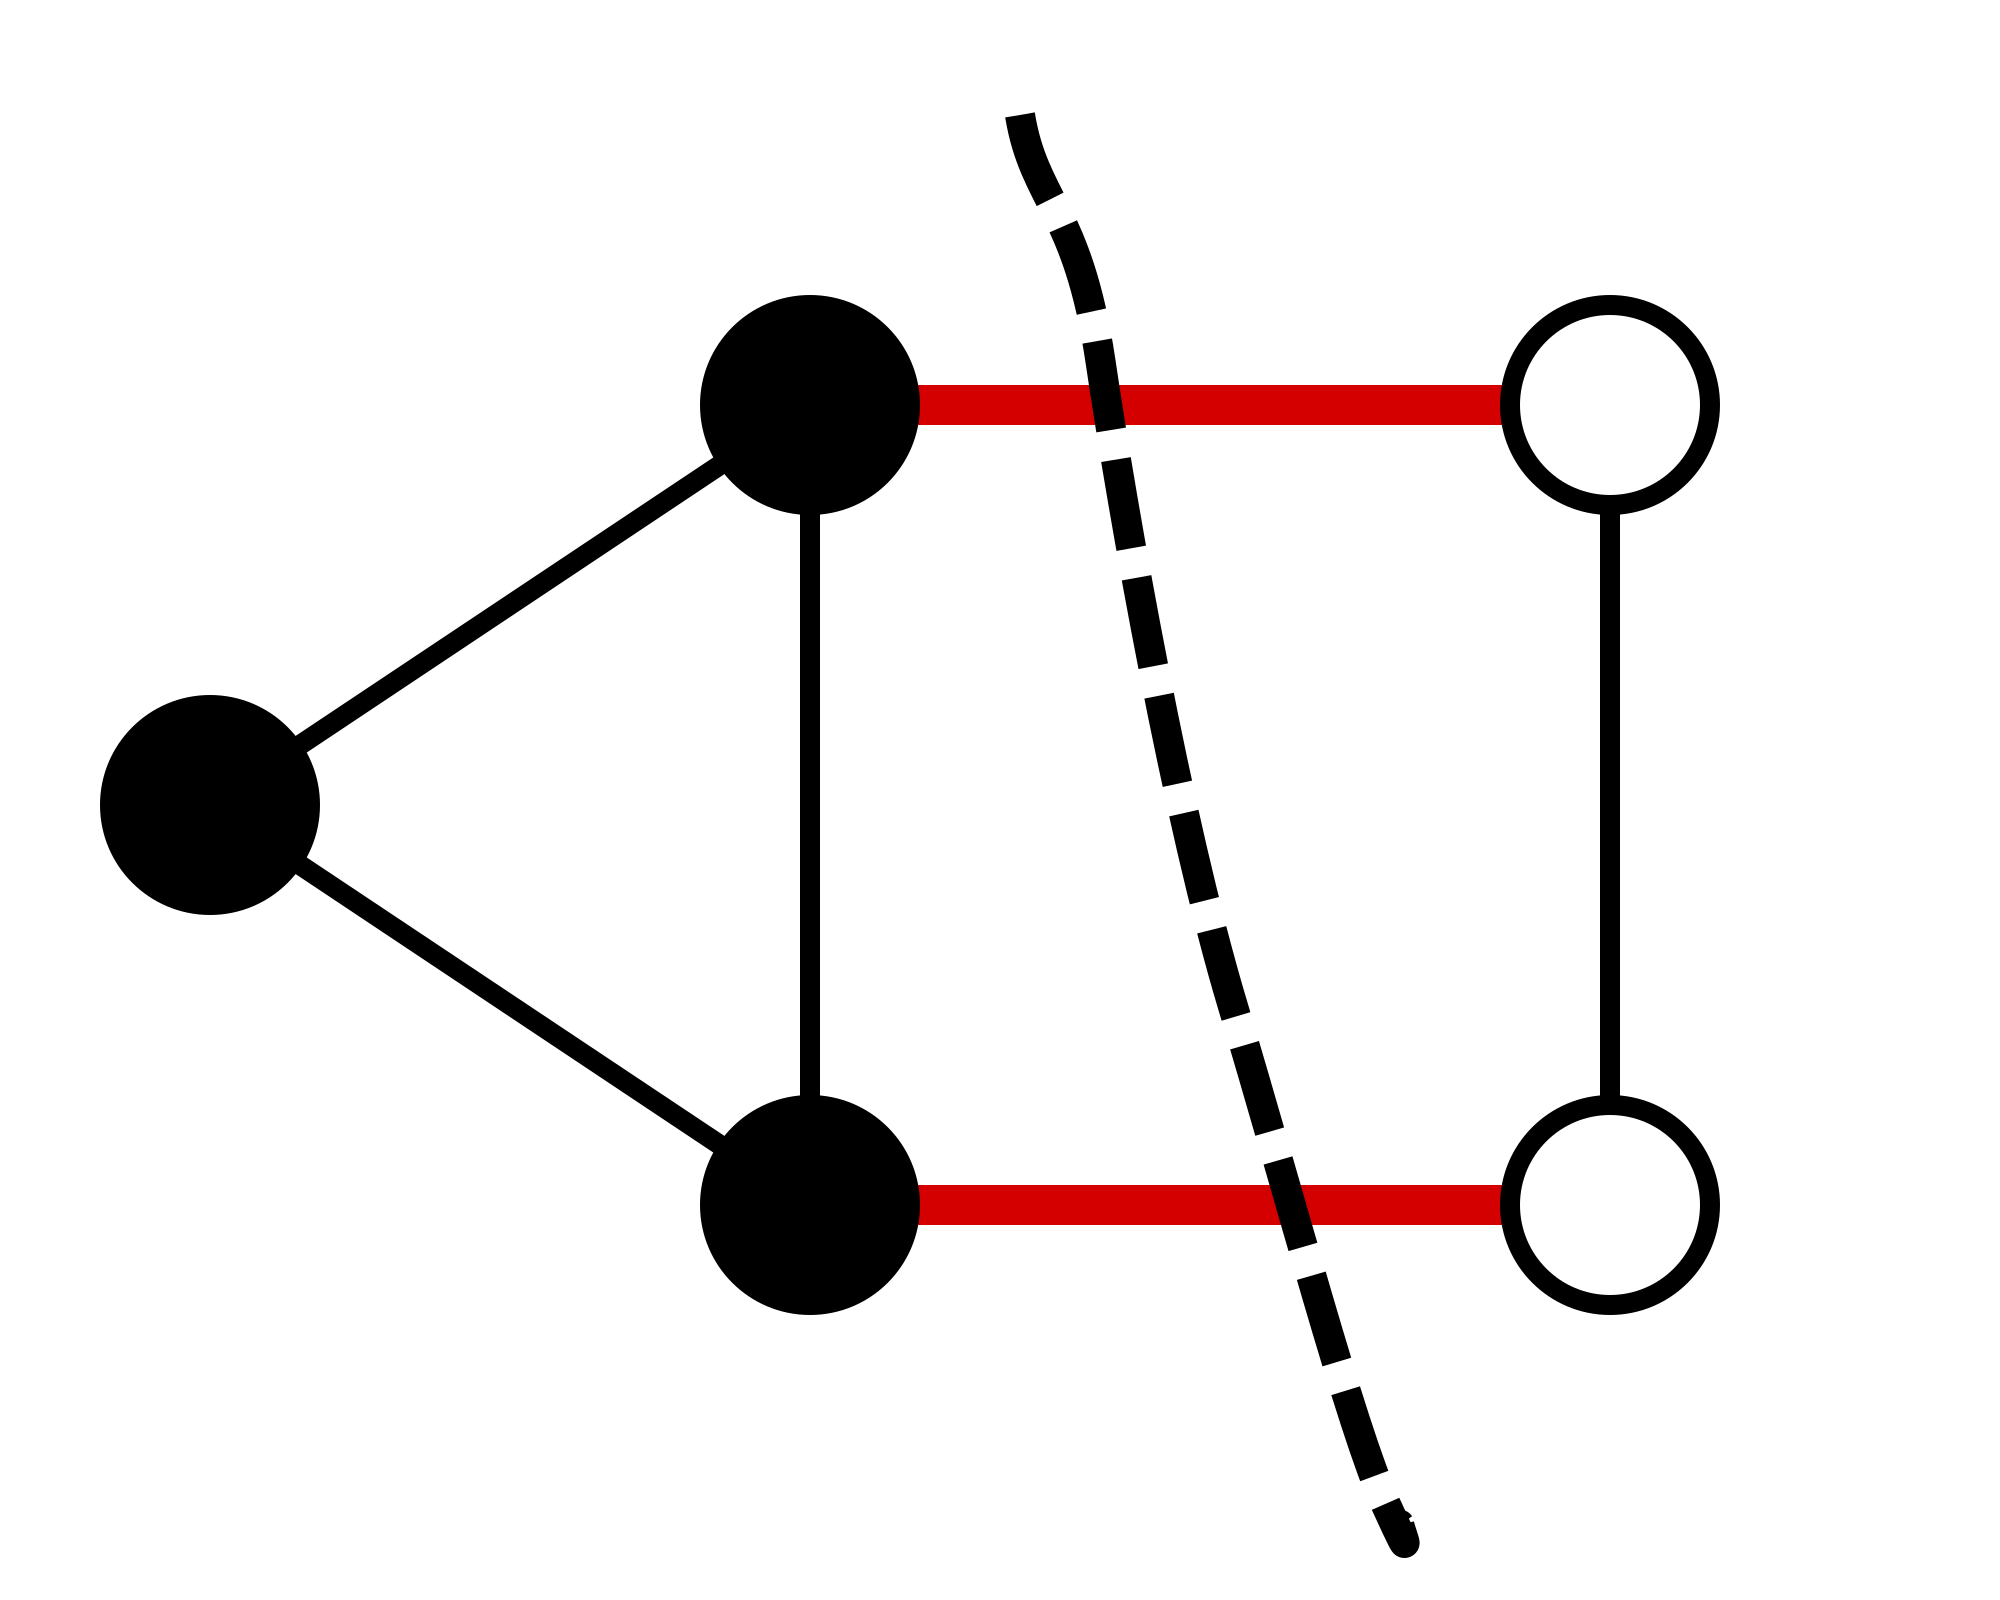
\includegraphics[width = .2\textwidth]{min_cut.png}}
				\subfloat[Maximum Cut]{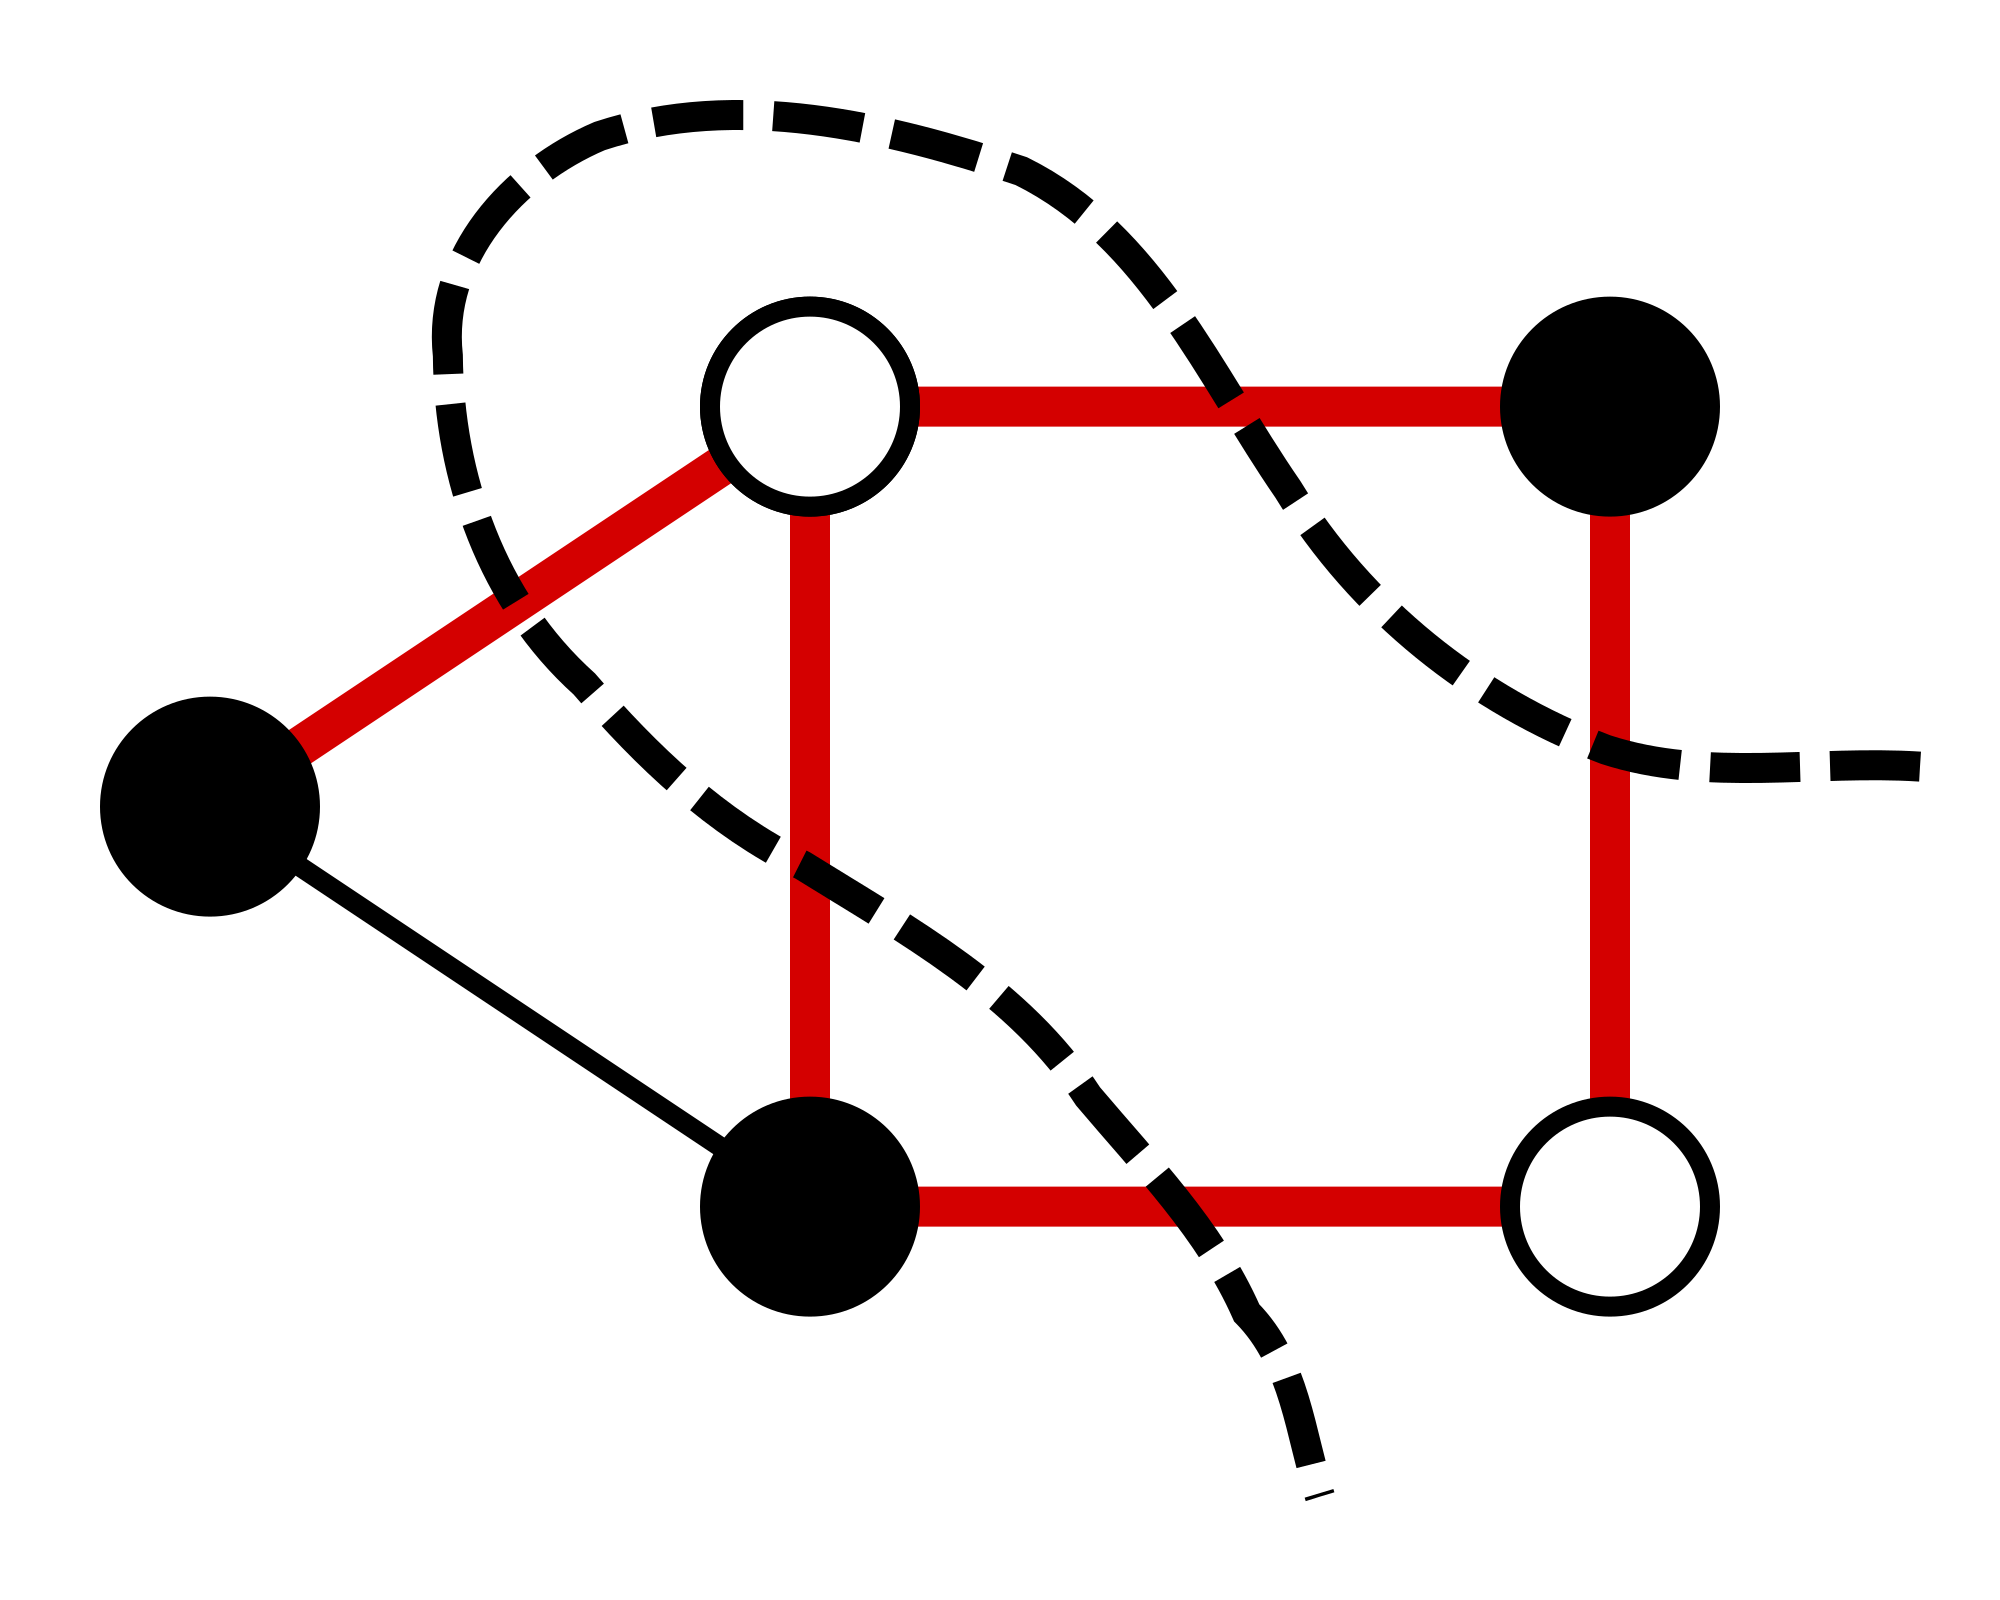
\includegraphics[width = .2\textwidth]{max_cut.png}}
				\caption*{}
			\end{center}
		\end{figure}
	}\label{definition:cut_graph_theory}
	
	
	\theo{https://en.wikipedia.org/wiki/Prufer_sequence}{Prufer sequence}{Consider a labeled tree $ T $ with vertices's $ \{1, 2, ..., n\} $. At step $ i $, remove the leaf with the smallest label and set the $ i $th element of the \textit{Prüfer sequence} to be the label of this leaf's neighbour. Prove that a Prüfer sequence of length $ n-2 $ defines a Tree with length $ n $.
		\fig{.2}{prufer_code_example}{A labeled tree with Prüfer sequence $ {4,4,4,5} $.}
	}



	\prob{https://artofproblemsolving.com/community/c6h5976p20088}{German TST 2004 E7P3}{M}{We consider graphs with vertices colored black or white. ``Switching" a vertex means: coloring it black if it was formerly white, and coloring it white if it was formerly black.\\
		
	Consider a finite graph with all vertices colored white. Now, we can do the following operation: Switch a vertex and simultaneously switch all of its neighbours (i. e. all vertices connected to this vertex by an edge). Can we, just by performing this operation several times, obtain a graph with all vertices colored black?}\label{problem:induction_type1_30}
	
	
		\solu{A classical example of creating complex moves from counter cases.}
		
		
	\prob{https://artofproblemsolving.com/community/c6h589936p3493453}{ARO 2014 P9.8}{H}{In a country of $ n $ cities, an express train runs both ways between any two cities. For any train, ticket prices either direction are equal, but for any different routes these prices are different. Prove that the traveler can select the starting city, leave it and go on, successively, $ n-1 $ trains, such that each fare is smaller than that of the previous fare. (A traveler can enter the same city several times.)}\label{tickets}
	
	
	\prob{https://artofproblemsolving.com/community/c6h364267}{Generalization}{\hrf{tickets}{H}}{Let $ A $ be a set of $ n $ points in the space. From the family of all segments with endpoints in $ A $ , $ q $ segments have been selected and colored yellow. Suppose that all yellow segments are of different length. Prove that there exists a polygonal line composed of $ m $ yellow segments, where $ m\geq\frac{2q}{n} $ , arranged in order of increasing length.}\label{problem:constructive_algo_9}\label{problem:swapping_4}
	
		\solu{Make one person go to every node. Then let the two people on the two sides of the most expensive edge swap their position. This ensures that every edge was used exactly 2 times. Using PHP, we have the desired result. Another solution is by \hrf{theorem:mirsky_theorem}{this}}
	
	
	
	\prob{}{}{E}{Given a bipartite graph, prove that the minimum number of colors required to color the edges of the graph such that no node is adjacent to $ 2 $ edges of same color is the maximum degree of the graph.}\label{problem:bipartite_graph_3}
	
	
	\prob{}{}{E}{For every bipartite graph prove that it's edges can be bicolored so that each node is adjacent to atmost $ \ceil{\dfrac{deg}{2}} $ edges of  any color.}\label{problem:bipartite_graph_4}
	
	
		\solu{Using the main property of a bipartite graph.}
	
	
		\solu{After finding the cycle solution, to optimize it, we recall that we can find a Eulerian Path (if it exists) in $ O(V+E) $. Now we want to make the graph have a Eulerian path, so we add a vertice to both sides of the graph, and join them with odd vertices from the other side.}
	
	
	
	
	\prob{https://artofproblemsolving.com/community/c6h100733p568964}{ISL 2005 C1}{E}{A house has an even number of lamps distributed among its rooms in such a way that there are at least three lamps in every room. Each lamp shares a switch with exactly one other lamp, not necessarily from the same room. Each change in the switch shared by two lamps changes their states simultaneously. Prove that for every initial state of the lamps there exists a sequence of changes in some of the switches at the end of which each room contains lamps which are on as well as lamps which are off.}\label{problem:divide_and_conquer_4}\label{problem:induction_type1_10}
	
	
	
	\prob{https://artofproblemsolving.com/community/c6h597130p3543398}{ISL 2013 C3}{M}{A crazy physicist discovered a new kind of particle which he called an $ i $ -mon, after some of them mysteriously appeared in his lab. Some pairs of $ i $ -mons in the lab can be entangled, and each $ i $ -mon can participate in many entanglement relations. The physicist has found a way to perform the following two kinds of operations with these particles, one operation at a time.
	
	\begin{enumerate}
		
		\item If some $ i $ -mon is entangled with an odd number of other $ i $ -mons in the lab, then the physicist can destroy it.
		
		\item At any moment, he may double the whole family of $ i $ -mons in the lab by creating a copy $ I' $ of each $ i $ -mon $ I $. During this procedure, the two copies $ I' $ and $ J' $ become entangled if and only if the original $ i $ -mons $ I $ and $ J $ are entangled, and each copy $ I' $ becomes entangled with its original $ i $ -mon $ I $ ; no other entanglements occur or disappear at this moment.
		
	\end{enumerate}
	
	Prove that the physicist may apply a sequence of much operations resulting in a family of $ i $ -mons, no two of which are entangled.
	}\label{problem:induction_type1_9}


		\solu{As there are an integer number of $ i $ -mons, it is quite natural to use induction. We try to find an algorithm to reduce the number of particles.
	
		Another way to do this is to consider the chromatic number of the graph. If we can show that this number reduces after some move, then we are done by induction.}



	\prob{https://artofproblemsolving.com/community/c6h104152p586762}{ISL 2005 C2}{E}{A forest consists of rooted (i. e. oriented) trees. Each vertex of the forest is either a leaf or has two successors. A vertex $ v $ is called an extended successor of a vertex $ u $ if there is a chain of vertices's $ u_{0}=u , u_{1}, u_{2} \dots u_{t-1} , u_{t}=v $ with $ t>0 $ such that the vertex $ u_{i+1} $ is a successor of the vertex $ u_{i} $ for every integer $ i $ with $ 0\leq i\leq t-1 $.\\
		
	Let $ k $ be a nonnegative integer. A vertex is called dynastic if it has two successors and each of these successors has at least $ k $ extended successors.\\
		
	Prove that if the forest has $ n $ vertices, then there are at most $ \frac{n}{k+2} $ dynastic vertices.}\label{problem:induction_type1_8}
	
		\solu{Trying to apply induction, we realize the bound is very loosy. That's why when we try to add in the inductive step, the value becomes larger than the bound. To stop that overflow, we tighten the bound.}
	
		\solu{The second and dummy approach is to first doing some smaller cases, finding small infos, taking the root, seeing that the bound doesnt work, but it would work if one of the successors of the root would have exactly or less than $ 2k+3 $ successors. As we can't always guarantee that, we look for such a vertex with $ 2k+3 $ successors. We do some work with it and by induction its done.}
	


	\prob{https://artofproblemsolving.com/community/c6h1441121p8200413}{All Russia 2017 9.1}{E}{In a country some cities are connected by oneway flights (There are no more then one flight between two cities). City $ A $ called "available" for city $ B $ , if there is flight from $ B $ to $ A $ , maybe with some transfers. It is known, that for every 2 cities $ P $ and $ Q $ exist city $ R $ , such that $ P $ and $ Q $ are available from $ R $. Prove, that exist city $ A $ , such that every city is available for $ A $.}\label{problem:induction_type1_17}
	
	
	
	\prob{www.google.com}{Jacob Tsimerman Induction}{E}{There are $ 2010 $ ninjas in the village of Konoha (what? Ninjas are cool.) Certain ninjas are friends, but it is known that there do not exist $ 3 $ ninjas such that they are all pairwise friends. Find the maximum possible number of pairs of friends.(If ninja $ A $ is friends with ninja $ B $ , then ninja $ B $ is also friends with ninja $ A $.)}\label{problem:induction_type1_16}


	\prob{https://artofproblemsolving.com/community/c6h420430p2374818}{USA TST 2011 D3P2}{M}{Let $n \geq 1$ be an integer, and let $S$ be a set of integer pairs $(a,b)$ with $1 \leq a < b \leq 2^n$. Assume $|S| > n \cdot 2^{n+1}$. Prove that there exists four integers $a < b < c < d$ such that $S$ contains all three pairs $(a,c)$, $(b,d)$ and $(a,d)$.}\label{problem:induction_type1_19}
	
		\solu{Using Induction to the first and last half of the set $ S $ shows us the \hrf{finding_the_tough_nut}{hardest part} of the problem. Then ordering the left and right elements with some sort of hierarchy is all the work left to do.}
	
	
	
	
	\prob{https://artofproblemsolving.com/community/c6h1480703p8639274}{ISL 2016 C6}{H}{There are $ n \geq 3 $ islands in a city. Initially, the ferry company offers some routes between some pairs of islands so that it is impossible to divide the islands into two groups such that no two islands in different groups are connected by a ferry route.\\
		
	After each year, the ferry company will close a ferry route between some two islands $ X $ and $ Y $. At the same time, in order to maintain its service, the company will open new routes according to the following rule: for any island which is connected to a ferry route to exactly one of $ X $ and $ Y $, a new route between this island and the other of $ X $ and $ Y $ is added.\\
		
	Suppose at any moment, if we partition all islands into two nonempty groups in any way, then it is known that the ferry company will close a certain route connecting two islands from the two groups after some years. Prove that after some years there will be an island which is connected to all other islands by ferry routes.}\label{problem:induction_type1_11}
	
		\solu{It is only natural to use induction on this kinda problems. After some trying, we see that if we remove $ 1 $ node, We get to nowhere, but if we remove $ 2 $ nodes, we get something interesting. So now focus on those two nodes and the rest of the nodes separately. Its not hard from there.}
	
		\solu{As it seems, the separation of the graph was the main observation. We can call this trick \hl{Bringing Order in the Chaos}.}



	\prob{https://artofproblemsolving.com/community/c6h535003p3067563}{ARO 2013 P9.5}{M (8/10)}{$ 2n $ real numbers with a positive sum are aligned in a circle. For each of the numbers, we can see there are two sets of $ n $ numbers such that this number is on the end. Prove that at least one of the numbers has a positive sum for both of these two sets.}\label{problem:graph_representation_4}\label{problem:minus_constant_2}
	
		\solu{Since there is nothing specfic about the sum, we may safely assume that it is $ 0 $, because (1) probably it works, and (2) it makes things more convenient. How we do that? we decrease every number by the average.\\
		
		Now, Consider every block of $ n $ consecutive blockes of numbers. When are two blocks connected? When they share the same end. What if we consider them as vertices, and this ``connectivity'' as edges? We see that cycles pop out.\\
		
		And we make use of the fact that our sum is $ 0 $. So signs are sure to bet flipped at the opposite side, and there are odd and even -ness in cycles that we can use.}
	
	
	
	
	\prob{https://artofproblemsolving.com/community/c6h420424p2374799}{USA TST 2011 P2}{HM (9/10)}{In the nation of Onewaynia, certain pairs of cities are connected by roads. Every road connects exactly two cities (roads are allowed to cross each other, e.g., via bridges). Some roads have a traffic capacity of 1 unit and other roads have a traffic capacity of $ 2 $ units. However, on every road, traffic is only allowed to travel in one direction. It is known that for every city, the sum of the capacities of the roads connected to it is always odd. The transportation minister needs to assign a direction to every road. Prove that he can do it in such a way that for every city, the difference between the sum of the capacities of roads entering the city and the sum of the capacities of roads leaving the city is always exactly one.}\label{problem:divide_and_conquer_1}\label{problem:induction_type2_3}
	
		\solu{As there are two types of subgraph, $ 1 $ -type and $ 2 $ -type. By some work-arounds, we see that we have to work distinctly in both types of graphs. Firstly, if we work in type- $ 1 $ , we see after making a path from node $ x, y $ , the degrees of $ x, y $ will be $ \{1, -1\} $ and the degrees of other nodes on the path will be the same. After that, we make every nodes have degree either $ \{1, -1\} $. So after this operation we remove the $ 1 $ -edges. Now, when dealing with the type- $ 2 $ sub-graph. Start over from zero, we see that when making a path between nodes $ x, y $ the degree of those two changes parity, and other nodes on the path stays the same. So select two odd nodes.... }
	
		\solu{Dealing with two different kind of edges simultaneously is messy, so we work with graph $ 1 $ and graph $ 2 $ differently. Now on both graphs, we can remove cycles. And in graph $ 2 $ , we see that we can remove any big paths if there is a edge $ 1 $ joining the two endpoints. Since if the new graph works then the previous graph works too. [Several cases to show here] And if there is no edge joining the two endpoints, replace the path by joining the two endpoints by a edge $ 2 $.\\
		
		Now there are only edge $ 1 $ s, and lone edge $ 2 $ s. Now dividing the graph $ 1 $ into paths of edge $ 1 $ , and dealing with several small cases, we are done.}
	
	
	
	\prob{https://artofproblemsolving.com/community/c6h276187p1494557}{Iran TST 2009 P6}{E-M (9/10)}{We have a closed path that goes from one vertex to another neighboring vertex, on the vertices of a $ n\times n$ square which pass throgugh each vertex exactly once. Prove that we have two adjacent vertices such that if we cut the path at these two points then the length of each open paths is at least $ n^2/4 $.}
	
		\solu{Draw a path, doesn't it look like a snake? Now can we relate the area of the tiled path with its perimeter? If we could do that, we would be able to replace two neighboring vertices by an edge inside the path, which seems to make the problem simpler.}
		
		
		
	\prob{https://math.stackexchange.com/questions/1439430/algorithm-to-uniquely-determine-a-number-using-two-adjacent-digits}{OC Chap2 P2}{M (6/10)}{Arutyun and Amayak perform a magic trick as follows. A spectator writes down on a board a sequence of $ N $ (decimal) digits. Amayak covers two adjacent digits by a black disc. Then Arutyun comes and says both closed digits (and their order). For which minimal $ N $ can this trick always work? NOTE: Arutyun and Amayak have a strategy determined beforehand.}\label{problem:bijection_2}\label{problem:hall_marriage_1}
	
		\solu{We have to actually find a bijection between all of the combinations the spectator can create, and all of the combinations that Arutyun might see when he comes back. Which tells us to use ``Perfect Matching" tricks.}
	
		\solu{Existential proof: for this trick to always work, they have to make a bijection from a set of $ N $ digits with two covered, to an unique set of $ N $ digits. Consider a bijection from the set of $ 0-9 $ strings with length $ N $ to the set of $ 0-9 $ strings with length $ N $ with $ 2 $ adjacent digits unknown. There exist a bijection iff the two sets satisfy Hall's Marriage Theorem. By double counting we get the value of $ N $ from here.}
	
	
	
	\prob{}{Simurgh 2019 P3}{E}{Call a graph \textit{symmetric}, if one can put its vertices on the plane such that it becomes symmetric wrt a line (which doesn't pass through any vertex). Find the minimum value of $ k $ such that (the edges of) every graph on $ 100 $ vertices, can be decomposed into $ k $ symmetric subgraph.}
	
	
	
	\prob{https://artofproblemsolving.com/community/c6h2019175p14186360}{RMM 2020 P3}{MH}{Let $n\ge 3$ be an integer. In a country there are $n$ airports and $n$ airlines operating two-way flights. For each airline, there is an odd integer $m\ge 3$, and $m$ distinct airports $c_1, \dots, c_m$, where the flights offered by the airline are exactly those between the following pairs of airports: $c_1$ and $c_2$; $c_2$ and $c_3$; $\dots$ ; $c_{m-1}$ and $c_m$; $c_m$ and $c_1$.
	
	Prove that there is a closed route consisting of an odd number of flights where no two flights are operated by the same airline.\index{Induction!Special!RMM 2020 P3}\index{Local!Add One by One!RMM 2020 P3}\index{Graph!Hall Marriage!RMM 2020 P3}\index{Graph!Bipartite!RMM 2020 P3}}

		\solu{[Weird Induction]
			Fix one vertice, merge all neighbors with it that has a unique airline between them.
		}
	
		\solu{[Element of Time]
			Add one edge from each cycle one at a time, without creating a cycle. Our objective is to show that when we reach the maximum stage where one edge creates a cycle, that cycle is of odd length.
		}

% \newpage\section{Game Theory}


	\begin{myitemize}
		\item \hrf{file:///home/ahsan/pDB/main/combi/GameTheoryPset.pdf}{Zawad's Game Theory Pset}
	\end{myitemize}
	

\subsection{Games}


	\den{Nimbers}{\href{file:///home/ahsan/pDB/main/combi/Game Theory/3.htm}{Nimbers} are simply `Nim values' which are assigned to a game configuration - these values are written as $ 0, *1, *2, *3 \dots $ We shall first describe how to obtain the Nim values for the game Squaring the Number. First, the Nim value of $ n=0 $ is assigned $ 0 $, since it is a state in which neither player has a valid move. We then recursively adopt the following rule for each $ n $ : \texttt{find all the possible moves from $ n $ and pick the smallest Nim value which does not occur among all these possible moves}.}


	\theo{file:///home/ahsan/pDB/main/combi/Game Theory/3.htm}{Sprague-Grund Theorem}{The \emph{Sprague–Grundy theorem} states that every impartial game under the normal play convention is equivalent to a nimber.}


	\khela{https://en.wikipedia.org/wiki/Chip-firing_game}{Chip Firing Game}{Let $ G=(V, E) $ be a graph without any loops or multiedges. Let a number of $ s_i $ chips be stacked on vertex $ i $. The game follows with the player choosing a vertex $ i $, taking $ d_i $ chips from it ($ s_i-d_i > 0 $), and sending one chip to each of the neighbors of the vertex where $ d_i $ is the degree of $ i $. The Problem of this game is to determine when the game will be infinte.
	\vspace{-1em}
		\begin{itemize}
			\item If $ N $ is the total number of edges in $ G $, and $ S $ is the total number of chips, then
	\end{itemize}}



	\khela{}{Cutting a stack in half}{Given a number of stacks, at his/her move, a player can choose a stack with even number stones, and divide it in two stacks with the same number of stones.}


	\khela{}{Cutting a stack in several}{Given a number of stacks, at his/her move, a player can choose a stack, and divide it in several stacks with the same number of stones.}






\newpage\subsection{Problems}



	\prob{https://artofproblemsolving.com/community/c5h202910p1116189}{USAMO 2008 P5}{M}{Three non-negative real numbers $ r_1 $ , $ r_2 $ , $ r_3 $ are written on a blackboard. These numbers have the property that there exist integers $ a_1 $ , $ a_2 $ , $ a_3 $ , not all zero, satisfying $ a_1r_1 + a_2r_2 + a_3r_3 = 0 $. We are permitted to perform the following operation: find two numbers $ x $ , $ y $ on the blackboard with $ x \le y $ , then erase $ y $ and write $ y - x $ in its place. Prove that after a finite number of such operations, we can end up with at least one $ 0 $ on the blackboard.}\label{problem:add_stuffs_2}

		\solu{When can't get info out of the reals, try the integers. Observe the integers, and check if they have any invariant. Rule of thumb of finding an invariant.}



	\prob{www.hehe.com}{USAMO 2014 P1}{E}{Let $ k $ be a positive integer. Two players $ A $ and $ B $ play a game on an infinite grid of regular hexagons. Initially all the grid cells are empty. Then the players alternately take turns with $ A $ moving first. In his move, $ A $ may choose two adjacent hexagons in the grid which are empty and place a counter in both of them. In his move, $ B $ may choose any counter on the board and remove it. If at any time there are $ k $ consecutive grid cells in a line all of which contain a counter, $ A $ wins. Find the minimum value of $ k $ for which $ A $ cannot win in a finite number of moves, or prove that no such minimum value exists.}\label{problem:coloring_1}

		\solu{Trying to block $ A $. We see that if we could alternately color the points black and white, we could've found some strategy for $ B $. But the triangle grid doesn’t seem very friendly. How can we color the triangles? And don't forget the details idiot.}




	\prob{www.hehe.com}{Indian TST 2004}{M}{The game of pebbles is played as followed: Initially there is one pebble at $ (0, 0) $. In a move one can remove the pebble at $ (i, j) $ and put one pebble each at $ (i+1, j) $ and $ (i, j+1) $ , given that both $ (i+1, j) $ and $ (i, j+1) $ were empty. Prove that at any point in the game, there will be a pebble at some lattice point $ (a, b) $ with $ a+b\leq 3 $.}\label{problem:invariant_rules_of_thumb_3}

		\solu{Two from one, means if the weight is reduced by half in the second level, then the sum would be the same.}





	\prob{https://artofproblemsolving.com/community/c6h18505p124463}{ISL 1998 C7}{H}{A solitaire game is played on an $ m\times n $ rectangular board, using $ mn $ markers which are white on one side and black on the other. Initially, each square of the board contains a marker with its white side up, except for one corner square, which contains a marker with its black side up. In each move, one may take away one marker with its black side up, but must then turn over all markers which are in squares having an edge in common with the square of the removed marker. Determine all pairs $ (m,n) $ of positive integers such that all markers can be removed from the board.}\label{problem:invariant_rules_of_thumb_4}

		\solu{If we remove one marker, then this cell becomes useless. So the neighbors to this cell will act like they are not connected to this cell. Now if a cell is connected to $ w $ white cells, and $ b $ black cells, then the resulting board state will have $ b-w $ more cells. Now only this info doesn't build up an invariant. Notice that as we are doing moves, we are reducing neighborhood relations as well, in other words, neighborhood relations decrease by $ b+w $. So if we consider the sum $ W+E $ where $ W $ is the number of all white cells, and $ E $ is the number of all neighborhood relations, we get an invariant on this value.}


	\prob{https://artofproblemsolving.com/community/c6h514376p2889829}{ARO 1999 P10.1}{E}{There are three empty jugs on a table. Winnie the pooh, Rabbit, and Piglet put walnuts in the jugs one by one. They play successively, with the initial determined by a draw. Thereby Winnie the pooh plays either in the first or second jug, Rabbit in the second or third, and Piglet in the first or third. The player after whose move there are exactly 1999 walnuts loses the games. Show that Winnie the pooh and Piglet can cooperate so as to make Rabbit lose.}

	
	\prob{https://artofproblemsolving.com/community/c6h5393p17438}{USAMO 2004, P4}{E}{Alice and Bob play a game on a $ 6 $ by $ 6 $ grid. On his or her turn, a player chooses a rational number not yet appearing in the grid and writes it in an empty square of the grid. Alice goes first and then the players alternate. When all squares have numbers written in them, in each row, the square with the greatest number in that row is colored black. Alice wins if she can then draw a line from the top of the grid to the bottom of the grid that stays in black squares, and Bob wins if she can't. (If two squares share a vertex, Alice can draw a line from one to the other that stays in those two squares.) Find, with proof, a winning strategy for one of the players.}
	
	
	
	
	\prob{https://artofproblemsolving.com/community/c6h1789908p11836140}{RMM 2019 P1}{E}{Amy and Bob play the game. At the beginning, Amy writes down a positive integer on the board. Then the players take moves in turn, Bob moves first. On any move of his, Bob replaces the number $n$ on the blackboard with a number of the form $n-a^2$, where a is a positive integer. On any move of hers, Amy replaces the number $n$ on the blackboard with a number of the form $n^k$, where $k$ is a positive integer. Bob wins if the number on the board becomes zero. Can Amy prevent Bob’s win?}
	
		\solu{Decent.}
		
		
	\prob{https://artofproblemsolving.com/community/c6h1268903p6622756}{ISL 2015 C4}{M}{Let $n$ be a positive integer. Two players $A$ and $B$ play a game in which they take turns choosing positive integers $k \le n$. The rules of the game are:
		
		\begin{enumerate}
			\item  A player cannot choose a number that has been chosen by either player on any previous turn.
			\item  A player cannot choose a number consecutive to any of those the player has already chosen on any previous turn.
			\item  The game is a draw if all numbers have been chosen; otherwise the player who cannot choose a number anymore loses the game.
		\end{enumerate}
		
	The player $A$ takes the first turn. Determine the outcome of the game, assuming that both players use optimal strategies.}
	
		\solu{Look at the simplest things, first produce data like a good boy, and then see what $ A $ has to do to win, or at least draw that he can't because $ B $ is an asshole.}
		
		
		
		
		
	\prob{https://artofproblemsolving.com/community/c6h546171p3160567}{ISL 2012 C4}{EM}{Players $A$ and $B$ play a game with $N \geq 2012$ coins and $2012$ boxes arranged around a circle. Initially $A$ distributes the coins among the boxes so that there is at least $1$ coin in each box. Then the two of them make moves in the order $B,A,B,A,\ldots $ by the following rules:
		\begin{enumerate}
			\item On every move of his $B$ passes $1$ coin from every box to an adjacent box.
			\item On every move of hers $A$ chooses several coins that were not involved in $B$'s previous move and are in different boxes. She passes every coin to and adjacent box.
		\end{enumerate}
	Player $A$'s goal is to ensure at least $1$ coin in each box after every move of hers, regardless of how $B$ plays and how many moves are made. Find the least $N$ that enables her to succeed.}

		\solu{Investigate $ B $'s move, see how and where he can make $ 0 $'s}
		
		
		
		
		
	\prob{https://artofproblemsolving.com/community/c6h355783p1932923}{ISL 2009 C1}{E}{Consider $ 2009 $ cards, each having one gold side and one black side, lying on parallel on a long table. Initially all cards show their gold sides. Two player, standing by the same long side of the table, play a game with alternating moves. Each move consists of choosing a block of $ 50 $ consecutive cards, the leftmost of which is showing gold, and turning them all over, so those which showed gold now show black and vice versa. The last player who can make a legal move wins.
		\vspace{-1em}
		\begin{enumerate}
			\itemsep-.5em
			\item  Does the game necessarily end?
			\item  Does there exist a winning strategy for the starting player?
	\end{enumerate}}\label{problem:extremal_case_whole_3}
	
	\rem{Trying out small cases doesn't help in this problem. Rather exploring what inevitably has to happen helps to notice patterns.}
	
	\solu{The first part of the problem is trivial induction usage.
		
		For the second half, notice that card $ 1 $ has to chosen only once. And cards $ 2, \dots 50 $ have to chosen an even number of times each. Again, card $ 51 $ has to be taken an odd number of times. Inductively, cards $ 1, 51 \dots 1951 $ were chosen odd number of times each, and all other cards were chosen even number of times each. Since that means the parity of total number of moves in this game is even.}
% \graphicspath{{Pics/combi/geo/}}

\newpage
\section{Combinatorial Geometry}


\begin{myitemize}
\item \href{https://blogm4e.files.wordpress.com/2016/08/combinatorial-geometry-maria-monks-mop-2010.pdf}{Combinatorial Geometry - Maria Monk (MOP 2010)}
\end{myitemize}


\begin{take_note*}{}
    \begin{itemize}[wide=0pt]
        \item Consider the convex hull made up of the points.
        \item Consider the extreme points: smallest or highest $ x $ or $ y $ coordinate.
        \item Find the triangle (quadrilateral, pentagon, etc.)  with the vertices being the points from your set $ S $, so that the area of the triangle is minimal/maximal.
    \end{itemize}
\end{take_note*}

\theo{https://en.wikipedia.org/wiki/Helly's_theorem}{Helly's Theorem}{Let $ X_1, ..., X_n $ be a finite collection of convex subsets of $ \R^d $, with $ n > d $. If the intersection of every $ d + 1 $ of these sets is nonempty, then the whole collection has a nonempty intersection; that is,
\[\bigcap _{j=1}^{n}X_{j}\neq \varnothing\]}


\vspace{1em}

\begin{myitemize}
    \item \href{https://math.berkeley.edu/~moorxu/misc/equiareal.pdf}{Sperner's
        Lemma - Moor Xu}
\end{myitemize}

\theo{https://www.wikiwand.com/en/Sperner's_lemma}
{Sperner's Lemma}{
    Given a triangle $ABC$, and a triangulation $\mathcal{T}$ of the triangle,
    the set $S$ of vertices of $\mathcal{T}$ is colored with three colors in
    such a way that
    \begin{enumerate}
        \item $A, B$, and $C$ are colored $1, 2$, and $3$ respectively.
        \item Each vertex on an edge of $ABC$ is to be colored only with one of the
            two colors of the ends of its edge. For example, each vertex on $AC$
            must have a color either $1$ or $3$.
    \end{enumerate}
    Then there exists a triangle from $\mathcal{T}$, whose vertices are colored with the
    three different colors. More precisely, there must be an odd number of
    such triangles. 
}


\begin{prooof}
    Consider a graph $G$ built from the triangulation $\mathcal{T}$ as
    follows:\\

    {\color{solC}The vertices of $G$ are the members of $\mathcal{T}$ plus the
    area outside the triangle.  Two vertices are connected with an edge if
    their corresponding areas share a common border with an edge $1$--$2$.\\}

    Note that on the interval $AB$ there is an odd number of borders colored
    $1$--$2$. Therefore, the vertex of $G$ corresponding to the outer area has
    an odd degree. \\

    But since in a finite graph there is an even number of
    vertices with odd degree, in the remaining graph, excluding the
    outer area, there is {\color{solC}an odd number of vertices with odd
    degree} corresponding to members of $\mathcal{T}$.\\

    It can be easily seen that the only possible degree of a triangle from
    $\mathcal{T}$ is $0, 1$, or $2$, and that the degree $1$ corresponds to a
    triangle colored with the three colors $1, 2$, and $3$.\\

    Thus we have obtained a slightly stronger conclusion, which says that in a
    triangulation $\mathcal{T}$ there is an odd number (and at least one) of
    full-colored triangles. 
\end{prooof}


\theo{https://www.wikiwand.com/en/Brouwer_fixed-point_theorem}
{Brouwer fixed-point theorem}{
    Let $B^n$ be the $n$th dimensional ball. Then any continuous map
    $f:B^n \to B^n$ has a fixed point.
}


\theo{}
{Equiareal Triangulation of a Square}{
    If we triangulate a square with triangles of equal area, then there must
    be an even number of triangles used.
}





\newpage
\subsection{Problems}

\prob{https://artofproblemsolving.com/community/c6h535002p3067558}{ARO 2013 P9.4}{E}{$ N $ lines lie on a plane, no two of which are parallel and no three of which are concurrent. Prove that there exists a non-self-intersecting broken line $ A_1A_2A_3\dots A_N $ with $ N $ parts, such that on each of the $ N $ lines lies exactly one of the $ N $ segments of the line.}\label{problem:constructive_algo_8}\label{problem:induction_type1_7}



\prob{https://artofproblemsolving.com/community/c6h1424941p8024557}{EGMO 2017 P3}{M}{There are $ 2017 $ lines in the plane such that no three of them go through the same point. Turbo the snail sits on a point on exactly one of the lines and starts sliding along the lines in the following fashion: she moves on a given line until she reaches an intersection of two lines. At the intersection, she follows her journey on the other line turning left or right, alternating her choice at each intersection point she reaches. She can only change direction at an intersection point. Can there exist a line segment through which she passes in both directions during her journey?}\label{problem:plane_coloring_1}

\solu{The condition that tells us to go either right or left, seems very non-rigorous. So to rigorize this condition, instead of using right or left condition in the direction, we consider what’s on our right and left. (INTUITION) After some experiment we see (not all of us) that if we color the plane with two colors in a way where every neighboring regions have different colors, we find some interesting stuff. (CREATIVITY) With this we are done. \hrf{plane_coloring}{Color the Plane}}





\prob{https://artofproblemsolving.com/community/c6h101306p571973}{ISL 2006 C2}{TE}{Let $ P $ be a regular $ 2006 $ -gon. A diagonal is called good if its endpoints divide the boundary of $ P $ into two parts, each composed of an odd number of sides of $ P $. The sides of $ P $ are also called good.

Suppose $ P $ has been dissected into triangles by $ 2003 $ diagonals, no two of which have a common point in the interior of $ P $. Find the maximum number of isosceles triangles having two good sides that could appear in such a configuration.}\label{problem:induction_type2_4}\label{problem:bijection_9}


\solu{The straight way, induction.}

\solu{The intuitive way, bijection. There are at most $ n $ good triangles, there are $ 2n $ edges, so a mapping that takes a two edges to a single good triangle must exist. Finding it is not that hard.}



\prob{https://artofproblemsolving.com/community/c6h589865p3493114}{ARO 2014 P9.3}{E}{In a convex $ n $ -gon, several diagonals are drawn. Among these diagonals, a diagonal is called good if it intersects exactly one other diagonal drawn (in the interior of the $ n $ -gon). Find the maximum number of good diagonals.}\label{problem:induction_type2_1}

\solu{There can be two cases, two good diagonals intersecting each other, and no two good diagonals intersecting each other. In the first case, we just use induction, and in the later, all of the good diagonals create a ``triangulation'' of the polygon, which gives us the numbers.}


\prob{https://artofproblemsolving.com/community/c6h1181527p5720110}{ISL 2013 C2, IMO 2013 P2}{E}{A configuration of $ 4027 $ points in the plane is called Colombian if it consists of $ 2013 $ red points and $ 2014 $ blue points, and no three of the points of the configuration are collinear. By drawing some lines, the plane is divided into several regions. An arrangement of lines is good for a Colombian configuration if the following two conditions are satisfied:

    \begin{enumerate}

        \item No line passes through any point of the configuration.
        \item No region contains points of both colors.

    \end{enumerate}

Find the least value of $ k $ such that for any Colombian configuration of $ 4027 $ points, there is a good arrangement of $ k $ lines.}\label{problem:sandwiching_points_1}

\solu{Obviously a n00b would think about induction. The only problem occurs when the convex hull completely consists of red points. In this case, after some investigation, we should get the sandwiching two points idea.}

\solu{Another way of inductive approach is like this, as the problem condition says that no region contains points of both colors, which means if we connect any two red and blue points, some line must bisect this segment. Now \hrf{problem:convex_hull_1}{it is known} that there is non intersecting partition of the points in to red-blue segments. So suppose in such a partition, we draw bisectors of each segments. Now there will be some holes in this proof. We see that to fill these holes, we have to focus on two red points with their respective blue partners, and draw the two bisectors in a way that separates the two red points form the blue points. So to remove further holes, we get the sandwiching idea.}


\prob{https://artofproblemsolving.com/community/c6h366745p2018324}{ILL 1985}{E}{Let $A$ and $B$ be two finite disjoint sets of points in the plane such that no three distinct points in $A \cup B$ are collinear. Assume that at least one of the sets $A, B$ contains at least five points. Show that there exists a triangle all of whose vertices's are contained in $A$ or in $B$ that does not contain in its interior any point from the other set.}

\solu{Concentrating on one of the sets five points such that there is no other points of the same set inside the hull of those five points.}\label{problem:convex_hull_2}



\prob{https://artofproblemsolving.com/community/c6h79789p456611}{APMO 1999 P5}{M}{Let $S$ be a set of $2n+1$ points in the plane such that no three are collinear and no four concyclic. A circle will be called ``Good'' if it has $ 3 $ points of $S$ on its circumference, $n-1$ points in its interior and $n-1$ points in its exterior. Prove that the number of good circles has the same parity as $n$.}


\solu{When thinking about induction, got a feeling that double counting with the number of good circles going through pairs of points might be useful, because a good circle will be counted three times, if we can show that every pair has odd number of good circles, we are done. So, take a pair. Now we need to `sort' the points somehow. See that, we can't sort the points in a trivial way with numbers, so moving to angles. Now setting conditions for a point inside of a circle in terms of angles, we see amazing patter, and an easy way to calculate the number of good circle of that pair of points.}



\prob{https://artofproblemsolving.com/community/c6h1113183p5083543}{ISL 2014 C1}{E}{Let $ n $ points be given inside a rectangle $ R $ such that no two of them lie on a line parallel to one of the sides of $ R $. The rectangle $ R $ is to be dissected into smaller rectangles with sides parallel to the sides of $ R $ in such a way that none of these rectangles contains any of the given points in its interior. Prove that we have to dissect $ R $ into at least $ n + 1 $ smaller rectangles.}\label{problem:extreme_object_7}\label{problem:double_counting_3}

\solu{Work with the largest continuous segments, and their endpoints.}



\prob{https://artofproblemsolving.com/community/c6h195050p1071295}{ISL 2007 C2}{EM}{A rectangle $ D$ is partitioned in several ($ \ge2$) rectangles with sides parallel to those of $ D$. Given that any line parallel to one of the sides of $ D$, and having common points with the interior of $ D$, also has common interior points with the interior of at least one rectangle of the partition; prove that there is at least one rectangle of the partition having no common points with $ D$'s boundary.}\label{problem:extreme_object_17}

\begin{minipage}{.6\linewidth}
    \solu{
        There existing such a rectangle means that there is a rectangular region
        inside of the original rectangle. So what if we walked along the segments,
        and cut a smaller rectangle from the inside of the rectangle? Like the way
        in the game.
    }
\end{minipage}\hfill%
\begin{minipage}{.4\linewidth}
    \figdf{.8}{2007c2}{}
\end{minipage}


\solu{Starting from one corner, and taking the opposite corner of the rectangle containing that corner, we use infinite decent to reach a contradiction.}

\solu{Using \hrf{problem:extreme_object_7}{ISL 2014 C1} as a lemma.}

\solu{Take one side of the square. Take a ``sandwiched'' rectangle touching that side. If no such rectangle exists, then it's just a special case that can be dealt with ease.}



\prob{https://artofproblemsolving.com/community/c6h5753p18977}{ISL 2003 C2}{E}{Let $D_1,D_2\dots,D_n$ be closed discs in the plane. (A closed disc is the region limited by a circle, taken jointly with this circle.) Suppose that every point in the plane is contained in at most $2003$ discs $D_i$. Prove that there exists a disc $D_k$ which intersects at most $7\cdot 2003 - 1 = 14020$ other discs $D_i$.}

\solu{Just go with the natural idea.}

\prob{https://artofproblemsolving.com/community/c6h5785p19086}{ISL 2003 C3}{E}{Let $n \geq 5$ be a given integer. Determine the greatest integer $k$ for which there exists a polygon with $n$ vertices (convex or not, with non-selfintersecting boundary) having $k$ internal right angles.}\label{problem:double_counting_10}

\solu{double count}



\prob{https://artofproblemsolving.com/community/c6h1389042p7736716}{Tournament of Towns 2015S S4}{A convex$N-$gon with equal sides is located inside a circle. Each side is extended in both directions up to the intersection with the circle so that it contains two new segments outside the polygon. Prove that one can paint some of these new $2N$ segments in red and the rest in blue so that the sum of lengths of all the red segments would be the same as for the blue ones.}

\solu{Just use what's the most natural, POP, on one vertex point.}


\prob{https://artofproblemsolving.com/community/c6h145844p825495}{USAMO 2007 P2}{E}{A square grid on the Euclidean plane consists of all points $(m,n)$, where $m$ and $n$ are integers. Is it possible to cover all grid points by an infinite family of discs with non-overlapping interiors if each disc in the family has radius at least $5$?}


\begin{minipage}{.5\linewidth}
    \prob{https://artofproblemsolving.com/community/c6h1135648p5301617}
    {MEMO 2015 T4}{EM}{
        Let $N$ be a positive integer. In each of the $N^2$ unit squares of an
        $N\times N$ board, one of the two diagonals is drawn. The drawn
        diagonals divide the $N\times N$ board into $K$ regions. For each $N$,
        determine the smallest and the largest possible values of $K$.
    }
\end{minipage}\hfill%
\begin{minipage}{.4\linewidth}
    \figdf{.7}{MEMO2015T4}{}
\end{minipage}


\solu{An Algorithmic Approach: Consider each diagonal as $ 0 $ or $ 1 $, prove that the maximum configuration is the one with alternating $ 0, 1 $s and the minimum one is the one with all $ 0 $s.}

\solu{A Counting Approach: Just count and bound with the minimum areas of the regions.}


\prob{}{}{EM}{In every cells of a $ m\times n $ grid, one of the two diagonals are drawn. Prove that there exist a path on these diagonals from left to right or from up to bottom of the grid.}

\solu{First remove the cycles, then take the largest path from left to right, and use induction.}



\prob{https://artofproblemsolving.com/community/c132h1546693p9385334}{Math Price for Girls 2017 P4}{E}{A lattice point is a point in the plane whose two coordinates are both integers. A lattice line is a line in the plane that contains at least two lattice points. Is it possible to color every lattice point red or blue such that every lattice line contains exactly 2017 red lattice points? Prove that your answer is correct.}

\solu{Transfinite induction.}


\prob{https://artofproblemsolving.com/community/c6h1217113p6063817}{China TST 2016 T3P2}{E}{In the coordinate plane the points with both coordinates being rational numbers are called rational points. For any positive integer $n$, is there a way to use $n$ colours to colour all rational points, every point is coloured one colour, such that any line segment with both endpoints being rational points contains the rational points of every colour?}

\solu{Transfinite induction}



\prob{https://artofproblemsolving.com/community/c6h1709989p11022201}{IGO 2018 A3}{E}{Find all possible values of integer $n > 3$ such that there is a convex $n$-gon in which, each diagonal is the perpendicular bisector of at least one other diagonal.}

\solu{Taking maximum terminal triangle.}


\prob{}{Lithuania ??}{E}{Prove that in every polygon there is a diagonal that cuts off a triangle and lies completely within the polygon.}


\prob{https://artofproblemsolving.com/community/c6h202941p1116402}{Romanian TST 2008 T1P4}{E}{Prove that there exists a set $ S$ of $ n - 2$ points inside a convex polygon $ P$ with $ n$ sides, such that any triangle determined by $3$ vertices of $ P$ contains exactly one point from $ S$ inside or on the boundaries.}

\solu{Checking small cases inductively quickly shows a construction.}


\prob{}{Iran TST ??}{E}{In an isosceles right-angled triangle shaped billiards table, a ball starts moving from one of the vertices adjacent to hypotenuse. When it reaches to one side then it will reflect its path. Prove that if we reach to a vertex then it is not the vertex at initial position}


\prob{https://artofproblemsolving.com/community/c6h1662915p10561203}{APMO 2018 P4}{EM}{Let $ABC$ be an equilateral triangle. From the vertex $A$ we draw a ray towards the interior of the triangle such that the ray reaches one of the sides of the triangle. When the ray reaches a side, it then bounces off following the law of reflection, that is, if it arrives with a directed angle $\alpha$, it leaves with a directed angle $180^{\circ}-\alpha$. After $n$ bounces, the ray returns to $A$ without ever landing on any of the other two vertices. Find all possible values of $n$.}


\solu{Reflect the whole board when just reflecting the ball doesn't seem to be helping. GLOBAL}



\prob{https://artofproblemsolving.com/community/c6h195043p1071276}{ISL 2007 C5}{EM}{In the Cartesian coordinate plane define the strips $ S_n = \{(x,y)|n\le x < n + 1\}$, $ n\in\mathbb{Z}$ and color each strip black or white. Prove that any rectangle which is not a square can be placed in the plane so that its vertices have the same color.}

\solu{Proceed step by step. See what happens if the parity of $ a, b $ are different. Then the case with two coprimes. In this case, we want to tilt the rectangle to some extent where the desired result is achieved. We just need to show that this is possible. A bit of wishful thinking and a bit of algebra does the rest.}	



\prob{https://artofproblemsolving.com/community/c6h1662910p10561186}{APMO 2018 P3}{M}{A collection of $n$ squares on the plane is called tri-connected if the following criteria are satisfied:

    \begin{enumerate}
        \item  All the squares are congruent.
        \item  If two squares have a point $P$ in common, then $P$ is a vertex of each of the squares.
        \item  Each square touches exactly three other squares.
    \end{enumerate}

How many positive integers $n$ are there with $2018\leq n \leq 3018$, such that there exists a collection of $n$ squares that is tri-connected?}

\solu{Play around to find that $ 6k $ for $ k>4 $ is good. Then play around a little bit more for a different construction. Another construction for $ 6k $ gives rise to a construction for $ 10k $. Which integers can be written as a sum of $ 6k $ and $ 10k $?}




\prob{https://artofproblemsolving.com/community/c6h1082935p4768413}{Iran 2005}{E}{A simple polygon is one where the perimeter of the polygon does not intersect itself (but is not necessarily convex). Prove that a simple polygon $P$ contains a diagonal which is completely inside $P$ such that the diagonal divides the perimeter into two parts both containing at least $\frac{n}{3} - 1$ vertices. (Do not count the vertices which are endpoints of the diagonal.)}

\solu{Triangulate.}	




\prob{https://artofproblemsolving.com/community/c6h287860p1555907}{ISL 2008 C3}{E}{In the coordinate plane consider the set $ S$ of all points with integer coordinates. For a positive integer $ k$, two distinct points $ a$, $ B\in S$ will be called $ k$-friends if there is a point $ C\in S$ such that the area of the triangle $ ABC$ is equal to $ k$. A set $ T\subset S$ will be called $ k$-clique if every two points in $ T$ are $ k$-friends. Find the least positive integer $ k$ for which there exits a $ k$-clique with more than 200 elements.}

\solu{When does $ ax+by= c $ have integer solution? Fix one point as origin and check other points friendliness with other points.}





\prob{https://artofproblemsolving.com/community/c6h1112753p5079689}{ISL 2015 C2}{E}{We say that a finite set $\mathcal{S}$ of points in the plane is balanced if, for any two different points $A$ and $B$ in $\mathcal{S}$, there is a point $C$ in $\mathcal{S}$ such that $AC=BC$. We say that $\mathcal{S}$ is centre-free if for any three different points $A$, $B$ and $C$ in $\mathcal{S}$, there is no points $P$ in $\mathcal{S}$ such that $PA=PB=PC$.\\

    \begin{enumerate}
        \item Show that for all integers $n\ge 3$, there exists a balanced set consisting of $n$ points.
        \item Determine all integers $n\ge 3$ for which there exists a balanced centre-free set consisting of $n$ points.
\end{enumerate}}

\solu{Simple, think about circles, then think about ``center-free'' in a graph theoritic manner.}





\newpage
\subsection{Chessboard Pieces}


\lem{}{What is the maximum number of knights that can be placed on a chessboard such that no two knights attack each other?}\label{lemma:maximum_knight_problem}

\solu{A knight's move always changes the color of the cell.}




\prob{https://artofproblemsolving.com/community/c6h1671290p10632348P}{IMO 2018 P4}{E/H}{A site is any point $(x, y)$ in the plane such that $x$ and $y$ are both positive integers less than or equal to 20.\\

    Initially, each of the 400 sites is unoccupied. Amy and Ben take turns placing stones with Amy going first. On her turn, Amy places a new red stone on an unoccupied site such that the distance between any two sites occupied by red stones is not equal to $\sqrt{5}$. On his turn, Ben places a new blue stone on any unoccupied site. (A site occupied by a blue stone is allowed to be at any distance from any other occupied site.) They stop as soon as a player cannot place a stone.\\

Find the greatest $K$ such that Amy can ensure that she places at least $K$ red stones, no matter how Ben places his blue stones.}\label{problem:coloring_3}


\solu{Using the \hrf{lemma:maximum_knight_problem}{maximum knight problem} as a lemma.}



\prob{}{}{E}{How many rooks can be placed on an $ n\times n $ board such that each rook attacks at most one other rook?}

\solu{Use graphs with one set of degrees being rows, and the other set of degrees being columns.}


\prob{https://en.wikipedia.org/wiki/Eight_queens_puzzle}{Eight queens puzzle}{}{How many queens can be placed on an $ n\times n $ board such that no queen attacks another queen?}

\begin{minipage}[t][][b]{0.195\linewidth}
    \figdf{1}{queen_88}{}
\end{minipage}\hfill%
\begin{minipage}[t][][b]{0.342\linewidth}
    \figdf{1}{queen_1414}{}
\end{minipage}\hfill%
\begin{minipage}[t][][b]{0.366\linewidth}
    \figdf{1}{queen_1515}{}
\end{minipage}\hfill%


\prob{https://artofproblemsolving.com/community/c6h1417932p7979120}{Serbia National D2P2}{HM}{How many queens can be placed on an $ n\times n $ board such that each queen attacks at most one other queen?}


\prob{}{BdMO 2019 P10}{E}{Define a new chess piece named warrior. it can either go three steps forward and one step to the side, or t2wo steps forward and two steps to the side in some orientation. In a $ 2020\times 2020 $ chessboard, prove that the mazimum number of warriors so that none of them attack each other is leass htan or equal to $ \dfrac{2}{5} $ of the number of cells.}

\solu{Color and partition}


\begin{minipage}{.5\linewidth}
    \prob{https://artofproblemsolving.com/community/c6h1790447p11841777}
    {RMM 2019 P4}{EM}{
        Prove that for every positive integer $n$ there exists a (not
        necessarily convex) polygon with no three collinear vertices, which
        admits exactly $n$ diffferent triangulations.

        (A triangulation is a dissection of the polygon into triangles by
        interior diagonals which have no common interior points with each
        other nor with the sides of the polygon)
    }
\end{minipage}\hfill%
\begin{minipage}{.4\linewidth}
    \figdf{.9}{RMM2019P4}{Fixes}
\end{minipage}





\prob{https://artofproblemsolving.com/community/c6h1062931p4608924}{China TST 2015 T1D2P1}{EM}{Prove that : For each integer $n \ge 3$, there exists the positive integers $a_1<a_2< \cdots <a_n$ , such that for $ i=1,2,\cdots,n-2 $ , With $a_{i},a_{i+1},a_{i+2}$ may be formed as a triangle side length , and the area of the triangle is a positive integer.}

\solu{First of all we dont need to limit us to integers, we can work with rationals. We want to build $ a_4 $ from $ a_1, a_2, a_3 $. with $ a_4> a_3 $ while keeping the area rational i.e. keeping the height and base rational.}



\prob{https://codeforces.com/problemset/problem/1158/D}{Codeforces 1158D}{E}{You are given $ n $ points on the plane, and a sequence $ S $ of length $ n-2 $ consisting of $ L $ and $ R $. You need to generate a sequence of the points $ a_1, a_2\dots a_n $ such that 
    \begin{itemize}
        \item the polyline $ a_1a_2\dots a_n $ is not self intersecting.
        \item the directed segment $ a_{i+1}a_{i+2} $ is on the left side of the the directed segment $ a_{i}a_{i+1} $ if $ S_i = L $, and on the right side if $ S_i = R $.
\end{itemize}}




% \newpage\section{Sequences}


\subsection{Lemmas}

\theo{https://en.wikipedia.org/wiki/Van_der_Waerden's_theorem}
{Van der Waerden's Theorem}{
    For any given positive integers $r$ and $k$, there is some number $ N $ such
    that if the integers $ \{1, 2, ..., N\} $ are colored, each with one of $ r $
    different colors, then there are at least $ k $ integers in arithmetic
    progression all of the same color.
}

\theo{}
{Catalan Recursion}{
    The infinite series defined as following: \[ a_0 = a_1 = 1,\ a_n =
    \prod_{i=0}^{n} a_ia_{n-i+1} = a_0a_{n-1} + a_1a_{n-2}\dots + a_{n-1}a_0 \]
    has the general term 
    \[a_n = C_n = \boxed{\frac{1}{n+1} \binom{2n}{n}}\] 
}



\subsection{Problems}


\begin{myitemize}
    \item \href{http://alexanderrem.weebly.com/uploads/7/2/5/6/72566533/sequences.pdf}{Sequences - Alexander Remorov}
\end{myitemize}

\prob{https://artofproblemsolving.com/community/c6h68945p404543}
{ISL 1990}{E}{
    Assume that the set of all positive integers is decomposed into $ r $
    (disjoint) subsets $ A_1 \cup A_2 \cup \dots \cup A_r = \mathbb{N}. $
    Prove that one of them, say $ A_i, $ has the following property: There
    exists a positive $ m $ such that for any $ k $ one can find numbers $
    a_1, a_2, \ldots, a_k $ in $ A_i $ with $ 0 < a_{j+1} - a_j \leq m, $  $
    (1 \leq j \leq k-1)$.
    \index[strat]{Induction!ISL 1990}
}


\prob{https://mathoverflow.net/questions/25313/finitely-many-arithmetic-progressions}
{Dividing the integers into arithmetic progressions, Erdos}{E}{
    Let $ d_1, d_2,\dots, d_k $ be differences of $ k $ arithmetic
    progressions that partition $ \N $. Show that $ d_i=d_j $ for some $i,j$.
    \index[strat]{Generating Function!Erdos, Arithmatic Progression}
    \index[strat]{Roots of unity filtering!Erdos, Arithmatic Progression}
}


\prob{https://artofproblemsolving.com/community/c6h79784p456601}
{APMO 1999 P1}{E}{
    Find the smallest positive integer $n$ with the following property: there
    does not exist an arithmetic progression of $1999$ real numbers containing
    exactly $n$ integers.
    \index[strat]{Name things!APMO 1999 P1}
}

\begin{solution}
    If the difference is $\frac{p}{q}$, then we can arrange the sequence in a
    way that we can get both exactly $\left\lfloor \frac{1999}{q} \right\rfloor$
    and $\left\lceil \frac{1999}{q} \right\rceil$ integers. \\

    So what we want is to find smallest integer $n$ for which there is a $k$
    such that
    \[n+1 \le \frac{1999}{k} \quad \text{ and } \quad \frac{1999}{k+1} \le n-1\] 
    So that $\frac{1999}{k}$ skips over $n$. After a bit of calculation, we
    get $n = 70, k = 28$ are the solutions we want.
\end{solution}


\prob{https://artofproblemsolving.com/community/c6h79787p456607}
{APMO 1999 P2}{E}{
    Let $a_1, a_2, \dots$ be a sequence of real numbers satisfying $a_{i+j}
    \leq a_i+a_j$ for all $i,j=1,2,\dots$. Prove that
    \[ a_1 + \frac{a_2}{2} + \frac{a_3}{3} + \cdots + \frac{a_n}{n} \geq a_n \]
    for each positive integer $n$.
    \index[strat]{Induction!APMO 1999 P2}
    \index[strat]{Sum them up!APMO 1999 P2}
}

\begin{solution}[jgnr]
    We will prove this by induction. Note that the inequality holds for $ n=1$. Assume that the inequality holds for $ n=1,2,\ldots,k$, that is,
\[ a_1\ge a_1,\quad a_1+\frac{a_2}2\ge a_2,\quad
    a_1+\frac{a_2}{2}+\frac{a_3}3\ge a_3, \quad \dots \quad
a_1+\frac{a_2}{2}+\frac{a_3}{3}+\cdots+\frac{a_k}k\ge a_k. \]
Sum them up:
\[ ka_1+(k-1)\frac{a_2}2a_2+\cdots+\frac{a_k}{k}\ge a_1+a_2+\cdots+a_k. \]Add $ a_1+\ldots+a_k$ to both sides:
\[ (k+1)\left(a_1+\frac{a_2}2+\cdots+\frac{a_k}k\right)\ge (a_1+a_k)+(a_2+a_{k-1})+\cdots+(a_k+a_1)\ge ka_{k+1}. \]
Divide both sides by $ k+1$:
\[ a_1+\frac{a_2}2+\cdots+\frac{a_k}k\ge\frac{ka_{k+1}}{k+1}, \] i.e.
\[ a_1 + \frac{a_2}{2} + \frac{a_3}{3} + \cdots + \frac{a_n}{n} \geq a_n. \]
\end{solution}


\prob{https://artofproblemsolving.com/community/c6h125791p713182}
{ISL 1994 A1}{E}{
    Let for each nonnegative integer $ n$, 
    \[ a_{0} = 1994 \quad a_{n + 1} = \frac {a_{n}^{2}}{a_{n} + 1}\] 
    Prove that $ 1994 - n$ is the greatest integer less than or equal to $
    a_{n}$, $ 0 \leq n \leq 998$
    \index[strat]{Rearrange!ISL 1994 A1}
    \index[strat]{Induction!ISL 1994 A1}
}

\solu{[t0rajir0u]
    Rewrite the condition as
    \[a_{n+1} = a_n -1 + \frac{1}{a_n + 1}\]
    Which gives us
    \[ a_{k} = 1994 - k + \frac {1}{a_{k - 1} + 1} + \frac {1}{a_{k - 2} + 1} +
    \dots + \frac {1}{1994 + 1}\]
    So we need to bound the fraction part below $1$ for $a_{998}$. By induction, it is
    atmost
    \[\frac{1}{997}+ \frac{1}{998}\dots + \frac{1}{1995}\] 
    Which is trivial to prove.
}


\prob{https://artofproblemsolving.com/community/c6h214669p1186971}
{ISL 2007 C4}{M}{
    Let $ A_0 = (a_1,\dots,a_n)$ be a finite sequence of real numbers. For
    each $ k\geq 0$, from the sequence $ A_k = (x_1,\dots,x_k)$ we construct a
    new sequence $ A_{k + 1}$ in the following way.
    \begin{enumerate}
        \item We choose a partition $ \{1,\dots,n\} = I\cup J$, where $ I$ and
            $ J$ are two disjoint sets, possibly empty, such that the expression 
            \[\left|\sum_{i\in I}x_i - \sum_{j\in J}x_j\right|\] 
            attains the smallest value. If there are several such partitions,
            one is chosen arbitrarily.
        \item We set $ A_{k + 1} = (y_1,\dots,y_n)$ where $ y_i = x_i + 1$ if
            $ i\in I$, and $ y_i = x_i - 1$ if $ i\in J$.
    \end{enumerate}
    Prove that for some $ k$, the sequence $ A_k$ contains an element $ x$
    such that $ |x|\geq\dfrac n2$.

    \index[strat]{Invariant!Sum of Squares!ISL 2007 C4}
}\label{problem:invariant_rules_of_thumb_11}

\solu{
    Suppose the contrary. Now, since $ A_i $ can only attain finite values, So $
    A_i = A_j $ for some $ i, j $. Now, we are taking about changes here, so we
    need to think of some invariants. Firstly the sum, it's not much of an help,
    because it doesn't give us much control. So kinda sum-ish invariant with a bit
    more control is the sum of squares. We combine these two ideas.
}



\prob{https://artofproblemsolving.com/community/c6h288840p1561573}
{ISL 2009 A6}{EM}{
    Suppose that $ s_1,s_2,s_3, \ldots$ is a strictly increasing sequence of
    positive integers such that the sub-sequences 
    \[s_{s_1},\, s_{s_2},\, s_{s_3},\, \ldots\quad\text{and}\quad
    s_{s_1+1},\, s_{s_2+1},\, s_{s_3+1},\, \ldots\] 
    are both arithmetic progressions. Prove that the sequence $ s_1, s_2, s_3,
    \ldots$ is itself an arithmetic progression.

    \index{Arithmetic Sequences!ISL 2009 A6}
    \index[strat]{Name things!ISL 2009 A6}
}

\solu{
    First notice that the two arithmetic sequences has the same common
    difference. Then notice that the diffrences of the original sequence is
    bounded.\\

    Another advice, give everything names. After naming the smallest
    difference and the largest differnce, we get two different inequalities,
    from where we deduce that the difference is constant.
}



\prob{https://artofproblemsolving.com/community/c6h1181540p5720240}
{ISL 2013 N2}{E}{
    Assume that $k$ and $n$ are two positive integers. Prove that there exist
    positive integers $m_1, \dots, m_k$ such that
    \[1+\frac{2^k-1}{n}=\left(1+\frac1{m_1}\right)\cdots \left(1+\frac1{m_k}\right).\]

    \index[strat]{Induction!ISL 2013 N2}
}

\solu{Just induct, and think wishfully.}



\prob{https://artofproblemsolving.com/community/c6t177f6h145842}
{USAMO 2007 P1}{E}{
    $n$ be a positive integer. Define a sequence by setting $a_1=n$ and, for each
    $k>1$, letting $a_k$ be the unique integer in the range $0\leq a_k \leq k-1$
    for which $a_0+a_1\dots +a_k$ is divisible by $k$. Prove that for any $n$ the
    sequence ${a_i}$ eventually becomes constant.

    \index[strat]{Invariant!Monovariant!USAMO 2007 P1}
}

\solu{Investigate and done.}


\prob{https://artofproblemsolving.com/community/c6h1071763p4663881}
{APMO 2015 P3}{E}{
    A sequence of real numbers $a_0, a_1, . . .$ is said to be good if the
    following three conditions hold.
    \begin{enumerate}[itemsep=5pt]
        \item The value of $a_0$ is a positive integer.
        \item For each non-negative integer $i$ we have $a_{i+1} = 2a_i + 1 $
            or $a_{i+1} =\dfrac{a_i}{a_i + 2} $
        \item There exists a positive integer $k$ such that $a_k = 2014$.
    \end{enumerate}
    Find the smallest positive integer $n$ such that there exists a good sequence
    $a_0, a_1, \dots$ of real numbers with the property that $a_n = 2014$.

    \index[strat]{Invariant!Monovariant!APMO 2015 P3}
    \index[strat]{Rearrange!APMO 2015 P3}
    \index[strat]{Get your hands dirty!APMO 2015 P3}
}

\solu{
    We will rename the sequence and call it $ \{s_i\} $, with $ s_0=x\in \Z $.
    Now let, \[s_i = \frac{a_ix+b_i}{c_ix+d_i}\]

    At the beginning we have $ a_0=d_0=1, b_0=c_0=0 $. It is easy to prove
    that \[ a_{i+1}+c_{i+1} = 2(a_i+c_i) \]\[ b_{i+1}+d_{i+1} = 2(b_i+d_i) \]
    So it follows that \[ a_i+c_i = 2^i = b_i+d_i \]
    Also, by induction (which is easy to prove), we have \[a_i - b_i = d_i - c_i = 1\]

    Suppose for some $ k $, $ s_k=2014 $. So, 
    \begin{align}
        &\frac{a_kx+b_k}{c_kx+d_k}=2014\\[1em]
        \implies x&=\frac{2014d_k-b_k}{a_k-2014c_k}=\frac{2015d_k-2^k}{2^k-2015c_k}\\[1em]
        &=\frac{2015(d_k-c_k)}{2^k-2015c_k}-1
    \end{align}

    But $ \gcd(2015, 2^k-2015c_k)=1 $, which implies $ 2^k-2015-c_k=1 $.
    Solving for $ k $ with CRT gives us $ 60|k $. 

    Now we have to prove that there is a sequence with $ s_{60} = 2014 $.
    Solving (1), $ s_0=2014 $, and,
    \[\begin{aligned}
        a_{60}&= \frac{2014\cdot 2^{60}+1}{2015} &b_{60} &=\frac{2014\cdot
        2^{60}-2014}{2015}\\[1em]
        c_{60}&= \frac{2^{60}-1}{2015} &d_{60} &=\frac{2^{60}+2014}{2015}
    \end{aligned}\]
    \vspace{1em}
    We show that we can make $ (a_{60}, c_{60}) $ from $ (a_0, c_0)=(1, 0) $.
    We prove it by induction, that $(a_k, c_k)$ can take any form $(2^k-i, i)$
    with $i\in\{0, 1, \dots 2^k-1\}$.
}


\prob{https://artofproblemsolving.com/community/c6h287853p1555896}
{ISL 2008 A4}{EM}{
    For an integer $ m$, denote by $ t(m)$ the unique number in $ \{1,    2,
    3\}$ such that $ m + t(m)$ is a multiple of $ 3$. A function $    f:
    \mathbb{Z}\to\mathbb{Z}$ satisfies $ f( - 1) = 0$, $ f(0) = 1$,    $ f(1)
    = - 1$ and $f\left(2^{n} + m\right) = f\left(2^n -    t(m)\right) - f(m)$
    for all integers $ m$, $ n\ge 0$ with $ 2^n >    m$. Prove that $ f(3p)\ge
    0$ holds for all integers $ p\ge 0$. 

    \index[strat]{Induction!ISL 2008 A4}
    \index[strat]{Get your hands dirty!ISL 2008 A4}
}

\begin{solution}
    We begin by listing values of $f(n)$ for $n\le 16$, and immediately it
    strikes us that:
    \begin{enumerate}
        \item  if $ -1\le x \le 2^{2m}-1$ then the maximal value is $
            f(2^{2m}-1)$ the minimal value is $ f(2^{2m}-2)$
        \item if $ -1\le x \le 2^{2m+1}$ then the maximal value is $ f(2^{2m+1}-2)$
            the minimal value is $ f(2^{2m+1}-1)$
    \end{enumerate}
    After which we are done by induction.
\end{solution}

% \newpage \subsection{Recurrent Sequences}	
	
	
	\begin{myitemize}
		\item \href{https://ufile.io/ywbniil2}{WOOT 2010-11 Recursion}
	\end{myitemize}
	
	
	\begin{BoxedTheorem}{Sum of Geometric Sequences}{}\label{theorem:Sum of Geometric Sequences}
		Every recurrent sequence can be written as a sum of some geometric sequences. Given a recurrent sequence, 
		\[x_n = a_1x_{n-1} + a_2x_{n-2}	+\dots + a_kx_{n-k}\]
		Then $ x_n $ can be written as 
		\[x_n = c_1r_1^n + c_2r_2^n +\dots + c_lr_l^n\]
		For all $ c_i $ if $ r_i $ are the roots of the \emph{characteristic polynomial} of the recursion. Which is:
		\[\tcboxmath[colback=white, colframe=white]{x^k - a_1x^{k-1} - a_2x^{k-2} \dots - a_k = 0}\]
		If there are double roots, say $ r_1 = r_2 = r_3 $, then we instead have,
		\[x_n = \tcboxmath[colback=white, colframe=white]{c_1r_1^n + c_2n\ r_2^n + c_3n^2\ r^n} \dots + c_lr_l^n\]
		 
		Reversely, we can say that a sequence defined by a sum of geometric recurrent series is a recursion. 
	\end{BoxedTheorem}

	\lem{}{Let $ F_n $ be the $ n $th Fibonacci number. Then the following holds:
		\[F_{n}^2 + F_{n+1}^2 = F_{2n+1}\]}
	
	\proof{Expanding the general form of the terms, and showing that $ a_n = F_{n}^2 + F_{n+1}^2 - F_{2n+1} $ is a recursion by \autoref{theorem:Sum of Geometric Sequences}.}
	
	\begin{BoxedTheorem}[title=Repertoire Method]{}{}
		Given a recurrent function defined by 
		\[f(n) = A(n)\a + B(n)\beta + C(n)\gamma\]
		We plug in different values for $ f(n) $, for example, $ f(n) = 1, n, 2n $ etc. for which the values are known from the recursion, and then solve for $ A, B, C $.
	\end{BoxedTheorem}
% \graphicspath{{Pics/combi/config/}}


\newpage\section{Exploring Configurations}

Problems where there is some kind of a configuration is given, the question
usually asks to proof or find some specific properties of the configuration.


\subsection{Problems}



\prob{https://artofproblemsolving.com/community/c6h1634977p10278658}{ARO 2018
    P11.5}{E}{
    On the table, there're $ 1000 $ cards arranged on a circle. On each
    card, a positive integer was written so that all $ 1000 $ numbers are
    distinct. 

    First, Vasya selects one of the card, remove it from the circle, and
    do the following operation: If on the last card taken out was written positive
    integer $ k $, count the $ k^{th} $ clockwise card not removed, from that
    position, then remove it and repeat the operation. This continues until only
    one card left on the table. 

    Is it possible that, initially, there's a card $A$ such that, no matter
    what other card Vasya selects as first card, the one that left is always
    card $A$?
}\label{problem:constructive_algo_7}

\solu{
    Consider the numbering, \[1, 1001!+1, 1002!+1, \dots 1998!+1,
    1999!+2\]It's easy to check that it works.
}

\rem{
    We want to find a configuration, where one card, let's call it $ a $,
    gets skipped over all the time. Now, controlling the skipping for every move
    is kinda hard. Instead of doing that, we want to control only one move that
    skips $ a $, and all other moves will go to the next card in the clockwise
    rotation. And the card before $ a $ will skip over $ a $, and land of the next
    card. That being said, the construction is rather trivial.
}


\prob{https://artofproblemsolving.com/community/c6h1446905p8271388}
{APMO 2017 P1}{M}{
    We call a $5$-tuple of integers arrangeable if its elements can be
    labeled $a,b,c,d,e$ in some order so that $a-b+c-d+e=29$. Determine all $ 2017$
    -tuples of integers $n_1, n_2, n_3\dots n_{2017}$ such that if we place
    them in a circle in clockwise order, then any $5$-tuple of numbers in
    consecutive positions on the circle is arrangeable.
}\label{problem:minus_constant_1}\label{problem:invariant_rules_of_thumb_5}

\solu{
    The annoying part is the $a-b+c-d+e = 29$ condition, as $29$ is too random.
    Can we do something to make this sum equal to a nicer interger, possibly
    $0$?
}



\prob{https://artofproblemsolving.com/community/c6h41116p258304}
{ISL 2004 C1}{E}{
    There are $10001$ students at an university. Some students join
    together to form several clubs (a student may belong to different clubs).
    Some clubs join together to form several societies (a club may belong to
    different societies). There are a total of $k$ societies. Find all
    possible values of $k$ so that the following conditions are satisfied:
    \begin{enumerate}
        \item  Each pair of students are in exactly one club.
        \item  For each student and each society, the student is in exactly
            one club of the society.
        \item  Each club has an odd number of students. In addition, a club
            with ${2m+1}$ students ($m$ is a positive integer) is in exactly $m$
            societies.  
    \end{enumerate}
}\label{problem:double_counting_7}

\solu{Just Double-Counting.}


\prob{https://artofproblemsolving.com/community/c6h17336p118710}{ISL 2002
C1}{E}{Let $ n $ be a positive integer. Each point $ (x,y) $ in the plane,
where $ x $ and $ y $ are non-negative integers with $ x+y<n $ , is coloured
red or blue, subject to the following condition: if a point $ (x,y) $ is red,
then so are all points $ (x',y') $ with $ x'\leq x $ and $ y'\leq y $. Let $ A
$ be the number of ways to choose $ n $ blue points with distinct $ x $
-coordinates, and let $ B $ be the number of ways to choose $ n $ blue points
with distinct $ y $ -coordinates. Prove that $ A=B
$.}\label{problem:induction_type1_5}\label{problem:recursive_solution_2}\label{problem:bijection_1}


\prob{https://artofproblemsolving.com/community/c5h476723p2669115}{USAMO 2012
P2}{M}{A circle is divided into $ 432 $ congruent arcs by $ 432 $ points. The
points are colored in four colors such that some $ 108 $ points are colored
Red, some $ 108 $ points are colored Green, some $ 108 $ points are colored
Blue, and the remaining $ 108 $ points are colored Yellow. Prove that one can
choose three points of each color in such a way that the four triangles formed
by the chosen points of the same color are
congruent.}\label{problem:double_counting_6}

\solu{Double counting saves the day :) The trick is to rotate ;)}



\prob{http://emc.mnm.hr/wp-content/uploads/2018/12/EMC_2018_Seniors_ENG_Solutions-2.pdf}{European
Mathematics Cup 2018 P1}{E}{Call a partition of $ n $ a set $ a_1, \dots a_k $
with $ a_1 \le a_2\dots \le a_k $ and $ a_1 + a_2 \dots + a_k =  $. A
partition of a positive integer is `even' if all of its elements are even
numbers. Similarly, a partition is `odd' if all of its elements are odd.
Determine all positive integers $ n $ such that the number of even partitions
of $ n $ is equal to the number of odd partitions of $ n $.}

\solu{Bijection.}


\prob{https://artofproblemsolving.com/community/c6h195492p1073989}{APMO 2008
P2}{EM}{Students in a class form groups each of which contains exactly three
members such that any two distinct groups have at most one member in common.
Prove that, when the class size is $ 46 $ , there is a set of $ 10 $ students
in which no group is properly
contained.}\label{problem:bijection_8}\label{problem:extremal_case_whole_5}

\solu{Taking the maximum set that follows the ``in which no group is properly
contained'' rule. Now the elements that are \emph{not} in this set, we can
connect this element to only one of the pairs from the set. Now defining a
bijection, and counting the elements, we are done.}



\prob{https://artofproblemsolving.com/community/c6h364231p2000940}{IMO SL
1985}{M}{A set of $ 1985 $ points is distributed around the circumference of a
circle and each of the points is marked with $ 1 $ or $ -1 $. A point is
called ``good'' if the partial sums that can be formed by starting at that
point and proceeding around the circle for any distance in either direction
are all strictly positive. Show that if the number of points marked with $ -1
$ is less than $ 662 $ , there must be at least one good
point.}\label{problem:induction_type1_12}

\solu{First thing to notice, the number $ 3*661 + 2 = 1985 $. And these
numbers are completely random. So what if we try to replace $ 1985 $ by $ n $
? Will the condition still hold?}


\prob{https://artofproblemsolving.com/community/c6h418978p2365036}{IMO 2011
P4}{E}{Let $ n > 0 $ be an integer. We are given a balance and $ n $ weights
of weight $ 2^0, 2^1, \cdots, 2^{n-1} $. We are to place each of the $ n $
weights on the balance, one after another, in such a way that the right pan is
never heavier than the left pan. At each step we choose one of the weights
that has not yet been placed on the balance, and place it on either the left
pan or the right pan, until all of the weights have been placed. Determine the
number of ways in which this can be done.}\label{problem:recursive_solution_5}

\solu{Writing the whole process as a sum, we see that only $ 2^0 $ is the odd
term here, if we remove that we can divide by $ 2 $ to get a recursive
formula.}

\solu{Calculating wrt to the last placed weight.}

\solu{Getting recursive formula considering the position of $ 2^{n-1} $.}





\prob{https://artofproblemsolving.com/community/c5h202936p1116367}{USAMO 2008
P3}{H}{Let $ n $ be a positive integer. Denote by $ S_n $ the set of points $
(x, y) $ with integer coordinates such that \[ \left\lvert x\right\rvert +
\left\lvert y + \frac{1}{2} \right\rvert < n. \] A path is a sequence of
distinct points $ (x_1 , y_1), (x_2, y_2), \ldots, (x_\ell, y_\ell) $ in $ S_n
$ such that, for $ i = 2, \ldots, \ell $ , the distance between $ (x_i , y_i)
$ and $ (x_{i-1} , y_{i-1} ) $ is $ 1 $ (in other words, the points $ (x_i,
y_i) $ and $ (x_{i-1} , y_{i-1} ) $ are neighbors in the lattice of points
with integer coordinates). Prove that the points in $ S_n $ cannot be
partitioned into fewer than $ n $ paths (a partition of $ S_n $ into $ m $
paths is a set $ \mathcal{P} $ of $ m $ nonempty paths such that each point in
$ S_n $ appears in exactly one of the $ m $ paths in $ \mathcal{P} $
).}\label{problem:alternating_chains_2}\label{problem:coloring_2}


\solu{Graph + Partition, coloring is just natural. Again, the edges join two
neighbor lattice points, so checkerboard coloring. But checkerboard doesn't do
much good. So the next thing we try is to apply some derivations of it,
pseudo!!! Well, overkill.}


\solu{For all n, induction is very natural. The optimal partition (the most
beautiful one) and the longest path in it, say $ P $ , gives us a way to
perform induction. As always, we suppose a partition with $ n-1 $ paths. As
there are a lot of partitions, we need to choose a certain partition, say $
\mathbb{M} $. Again as our goal is to include $ P $ in $ \mathbb{M} $. So
suppose that the set with all the points in $ P $ is $ A $. And further more,
suppose that in $ \mathbb{M} $ there is a path $ Q $ with $ \vert Q\cap A\vert
$ being maximal among all other partitions of the points. Some some easy case
work shows that we must have $ P\in \mathbb{M} $.}



\prob{https://artofproblemsolving.com/community/c5h532235p3041823}{USAMO 2013
P2}{H}{For a positive integer $ n\geq 3 $ plot $ n $ equally spaced points
around a circle. Label one of them $ A $ , and place a marker at $ A $. One
may move the marker forward in a clockwise direction to either the next point
or the point after that. Hence there are a total of $ 2n $ distinct moves
available; two from each point. Let $ a_n $ count the number of ways to
advance around the circle exactly twice, beginning and ending at $ A $ ,
without repeating a move. Prove that $ a_{n-1}+a_n=2^n $ for all $ n\geq 4
$.}\label{problem:recursive_solution_4}\label{problem:bijection_7}


\solu{Problems where there are multiple possible value of a function
regardless of the current position, one of dealing with these is to assigning
labels of these possible values to each points of the function, and this will
give a combinatorial model and a way to deal it with bijection.}

\solu{First investigate the problem condition, $ a_n + a_{n-1} = 2^n $ , now,
$ 2^n $ means the number of differently coloring every point black or white,
and the left side is the number of such paths for $ n $ and $ n-1 $. Which
means we should try to color the points and see what happens.}

\proof{EChen's solution: In this problem, the main obstacle seems to be the
circle condition. And on top of that, on can land on the starting point. So
things are pretty messed up here. What we want to do is to make things a
little bit more easy to deal with. So our best option is to change the problem
so that we get the similar problem with a different explanation. So we change
the condition circle with matrix, $ 2 $ round with $ 2 $ rows. $ n $ points
with $ n $ entries in each rows. What we get now is the same problem, just a
bit easier to deal with. We call this \hl{Tweak The Problem} strategy.}



\prob{}{}{E}{ $ 10 $ persons went to a bookstore. It is known that: Every
person has bought 3 kinds on books and for every 2 persons, there is at least
one kind of books which they both have bought. Let $ m_i $ be the number of
the persons who bought the $ i^{th} $ kind of books and $ M= \max\lbrace
m_i\rbrace $ Find the smallest possible value of $ M
$.}\label{problem:double_counting_4}


\prob{https://artofproblemsolving.com/community/c6h86560p504805}{ARO 2006
    11.3}{M}{On a $49\times 69$ rectangle formed by a grid of lattice squares,
    all $50\cdot 70$ lattice points are colored blue. Two persons play the
    following game: In each step, a player colors two blue points red, and
    draws a segment between these two points. (Different segments can
    intersect in their interior.) Segments are drawn this way until all
    formerly blue points are colored red. At this moment, the first player
    directs all segments drawn - i. e., he takes every segment AB, and
    replaces it either by the vector $\overrightarrow{AB}$, or by the vector
    $\overrightarrow{BA}$. If the first player succeeds to direct all the
    segments drawn in such a way that the sum of the resulting vectors is
    $\overrightarrow{0}$, then he wins; else, the second player wins.

Which player has a winning strategy?}

\proof{The basic idea comes from wishing that the first player might be able
to copy the second player to ``nullify'' his moves. But since this isn't
always possible, because no nice symmetry exists on the board, the idea of
coloring the board with dominoes and copying moves wrt the dominoes comes.
\index[strat]{copycat!partition!aro 2006 11.3}}


\prob{https://artofproblemsolving.com/community/c6h17338p118714}{ISL 2002
C3}{EM}{Let $n$ be a positive integer. A sequence of $n$ positive integers
(not necessarily distinct) is called full if it satisfies the following
condition: for each positive integer $k\geq2$, if the number $k$ appears in
the sequence then so does the number $k-1$, and moreover the first occurrence
of $k-1$ comes before the last occurrence of $k$. For each $n$, how many full
sequences are
there?}\label{problem:bijection_13}\label{problem:graph_representation_9}

\proof{After guessing the ans, the first thing that I did was to draw a level
based graph. Suppose that a full sequence has $ k $ different entries. Then
the top level contains the positions of $ k $ in the sequence sorted from left
to right. The next level contains the positions of $ k-1 $ in the sequence
sorted so, and so on till the last level. What I noticed is that if we draw
arrows pointing from a larger integer to a smaller integer, the only arrows
(or more like relations between entries of the sequence) we need to worry
about are the arrows pointing left to right in each levels, and the arrows
from the last entry of level $ i $ to the first entry of level $ i+1 $. After
this, if we try with a smaller case, we see that this leads to a bijection
from the set of sequences of length $ n $ with $ n $ different integers to the
set of full-sequences of length $ n $.}


\solu{Another bijection approach is as followed, in a full-sequence, on first
run, go from right to left, placing integers starting with $ 1 $ onwards on
the $ 1 $'s in the sequence. on the second run continue counting and placing
integers on the $ 2 $'s and so on.}


\solu{Another idea is to prove $ a_n = n a_{n-1} $. To do this, remove the
rightmost $ 1 $ and do some casework.}



\prob{https://artofproblemsolving.com/community/c6h219938p1219679}{ISL 1994
C2}{M}{In a certain city, age is reckoned in terms of real numbers rather than
integers. Every two citizens $x$ and $x'$ either know each other or do not
know each other. Moreover, if they do not, then there exists a chain of
citizens $x = x_0, x_1, \ldots, x_n = x'$ for some integer $n \geq 2$ such
that $ x_{i-1}$ and $x_i$ know each other. In a census, all male citizens
declare their ages, and there is at least one male citizen. Each female
citizen provides only the information that her age is the average of the ages
of all the citizens she knows. Prove that this is enough to determine uniquely
the ages of all the female citizens.}

\solu{Describing the problem using matrix and vector spaces, the problem
reduces to well known theorems of linear algebra.}


\prob{https://artofproblemsolving.com/community/c6h93p261}{ISL 2003 C1}{E}{Let
$A$ be a $101$-element subset of the set $S=\{1,2,\ldots,1000000\}$. Prove
that there exist numbers $t_1$, $t_2, \ldots, t_{100}$ in $S$ such that the
sets \[ A_j=\{x+t_j\mid x\in A\},\qquad j=1,2,\ldots,100 \] are pairwise
disjoint.}

\solu{just count...}


\prob{https://artofproblemsolving.com/community/c6h1425422p8029376}{EGMO 2017
    P5}{E}{Let $n\geq2$ be an integer. An $n$-tuple $(a_1,a_2,\dots,a_n)$ of
    not necessarily different positive integers is expensive if there exists a
    positive integer $k$ such that 

    \[(a_1+a_2)(a_2+a_3)\dots(a_{n-1}+a_n)(a_n+a_1)=2^{2k-1}\]

    a) Find all integers $n\geq2$ for which there exists an expensive
    $n$-tuple.

b) Prove that for every odd positive integer $m$ there exists an integer
$n\geq2$ such that $m$ belongs to an expensive $n$-tuple.}

\rem{gutaguti solution}

\solu{All odd $ n $ works, you can prove for even $ n $ by $ +1, -1 $
addition. For the second part, start with the odd number, move on both side,
you will eventually reach $ 1 $.}



\prob{https://artofproblemsolving.com/community/c6h84550p490581}{USAMO 2006
P2}{E}{For a given positive integer $k$ find, in terms of $k$, the minimum
value of $N$ for which there is a set of $2k + 1$ distinct positive integers
that has sum greater than $N$ but every subset of size $k$ has sum at most
$\tfrac{N}{2}.$}

\solu{Compactness is the optimal decision.}



\prob{https://artofproblemsolving.com/community/c6h1076949p4710743}{MOP
Problem}{E}{Prove that for any positive integer $c$, there exists an integer
$n$ such that $n$ has more 1's in its binary expansion than $n^2+c$ does.}

\solu{For $ x= 2^a-1 $, $ x $ and $ x^2 $ have the same number of $ 1's $. So
does $ x=2^a-2^b $. But what if increase the number of $ 1's $ in this $ x $
by substracting $ 1 $? Let $ x=2^a - 2^b -1 $. This might work if we can
choose nice $ a, b $'s}



\prob{https://artofproblemsolving.com/community/c6h1078552p4732509}{EGMO 2015
P2}{EM}{A domino is a $2 \times 1$ or $1 \times 2$ tile. Determine in how many
ways exactly $n^2$ dominoes can be placed without overlapping on a $2n \times
2n$ chessboard so that every $2 \times 2$ square contains at least two
uncovered unit squares which lie in the same row or column.}

\solu{Notice how each of the four kind of dominoes needs to be in a group. So
if we separated them into blocks, inverstigation shows that there can only be
$ 4 $ blocks and each strictly attached to the sides. The reason why this is
happening is pretty obvious. Now those blocks create two paths between the two
opposite vertices of the square. This gives our desired bijection.}



\prob{https://artofproblemsolving.com/community/c6h148826p841252}{USA TST 2006
P5}{TE}{Let $n$ be a given integer with $n$ greater than $7$ , and let
$\mathcal{P}$ be a convex polygon with $n$ sides. Any set of $n-3$ diagonals
of $\mathcal{P}$ that do not intersect in the interior of the polygon
determine a triangulation of $\mathcal{P}$ into $n-2$ triangles. A triangle in
the triangulation of $\mathcal{P}$ is an interior triangle if all of its sides
are diagonals of $\mathcal{P}$. Express, in terms of $n$, the number of
triangulations of $\mathcal{P}$ with exactly two interior triangles, in closed
form.}

\solu{Just mindless calculation...}



\prob{https://artofproblemsolving.com/community/c6h418687p2362298}{ISL 2010
    C3}{E}{2500 chess kings have to be placed on a $100 \times 100$ chessboard
    so that

    \begin{enumerate} \item  no king can capture any other one (i.e. no two
    kings are placed in two squares sharing a common vertex); \item  each row
    and each column contains exactly 25 kings.  \end{enumerate}

Find the number of such arrangements. (Two arrangements differing by rotation
or symmetry are supposed to be different.)}



\solu{In a $ 2\times 2 $ box, one can place only one king. So we divide the
board in that way, and explore...}



\prob{https://artofproblemsolving.com/community/c6h1558133_a_tasty_dish_of_graph_theory}{USA
    Winter TST 2018 P3}{M}{
    At a university dinner, there are $ 2017 $
    mathematicians who each order two distinct entrées, with no two mathematicians
    ordering the same pair of entrées. The cost of each entrée is equal to the
    number of mathematicians who ordered it, and the university pays for each
    mathematician's less expensive entrée (ties broken arbitrarily). Over all
    possible sets of orders, what is the maximum total amount the university could
    have paid?
}

	\begin{solution}[Grid Representation]
			We put the information in a grid in the usual manner. We take the configuration for which the score (which we define to be the total amount the university has to pay) is maximum.
			
			\begin{solution_def}
				Let $ C_i $ be the price of the dish $ i $. Let $ P_j $ be the pair of dishes $ j $ ordered.
			\end{solution_def}
			
			We now ``sort'' the grid in the following way:
			\begin{itemize}
				\item Sort the columns first, from the least expensive to the most.
				\item Now we have $ 2017 $ binary strings as rows. We sort them decreasingly from top to bottom.
			\end{itemize}
		
			We end up with something like this:
			\figdf{.3}{USA_TST_2018_P3_1}{}
			
			\begin{solution_def}
				We make some sets:\[ A_i=\{x| x \text{ ordered dish } i \text{ but didn't order any of the dishes } j<i\} \]Let $ a_i = |A_i| $.
				We also call $ A_i $ block, the $ x $th rows with $ x\in A_i $. It is easy to see that the committee has to pay for dish $ i $ $ a_i $ times.
			\end{solution_def}
		
			Take a $ j $ such that $ a_j=0 $.
			 
			If $ j<k $, let \[S_j = \{x\mid \text{In the } j^{th} \text{ column, there is a } 1 \text{ in the set of the rows from } A_x \}\]
				\figdf{.3}{USA_TST_2018_P3_2}{}
			In the example of the previous diagram, $ S_4 = \{1, 2, 3\} $
			
			Take the largest element of $ S_j $, namely $ t $. We want to move the $ 1 $ in the $ A_t $ block of column $ j $ to another column to the right. Notice that this won't decrease the score, because for each of the mathematician after the block $ A_t $, the score would be non decreasing. If we could do this, we could do this inductively, moving the $ j $th column to the left each move, eventually making it disappear. 
			
			So suppose we can't do this. So there is no column on the right of $ t $, that does not have a $ 1 $ in the block $ A_t $. It is straightforward to deduce that $ N=t+a_t $. 
			
			From there, we can say:
				\[a_{t+m}\le a_t-m\text{ and }a_{t-m}\le a_t+m\]
			So,
			\begin{align*}
				2017=\sum a_i &\le (a_t+t-1) +\dots 1 \\
				\implies 2017 &\le \frac{N(N-1)}{2}\\
				\implies N&\ge 65
			\end{align*}
			
			We know that the score, $ S= \sum C_ka_k $. where $ a_i $ is strictly decreasing and $ C_i $ is non decreasing. So the maximum sum would have $ C_i=K $ for some constant (by rearrangement inequality). And to have $ K $ maximum, we need $ N $ minimum or $ N=64 $. 
			
			And if $ j>k $, the same reason holds. So $ N=65, a_1=63, a_2=62\dots a_63=1 $. But we need another $ a_i=1 $, that has to be on its own. 
		\end{solution}

\rem{Easy to think in grids, but it was quite difficult to formulate the
solution rigorously, I still am not 100\% convinced myself. Next time when I
feel like it, I will reconstruct the solution. Roughly it is: take the final 0
value columns, prove that there is only one such, and prove the bounds on the
solution before using that instead. Then use general bounding to find the
maximum. It's not hard, it's just I don't have time now. GAH!! HSC!!}

\rem{Didn't read other solutions too, gonna give a todo}
%todo: read other solutions.


\subsubsection{Conway's Soldiers}


\prob{https://artofproblemsolving.com/community/c6h62194p372309}{ISL 1993
C5}{MH}{On an infinite chessboard, a solitaire game is played as follows: at
the start, we have $n^2$ pieces occupying a square of side $n.$ The only
allowed move is to jump over an occupied square to an unoccupied one, and the
piece which has been jumped over is removed. For which $n$ can the game end
with only one piece remaining on the board?}

\solu{We want to find an invariant. So we need to find a weight for each of
the cells such that any two consecutive cells' values equals to the values of
the two cells on the two sides. Some mind bashing gives the idea of mod $ 3 $.
And a construction for the other $ n $'s can be easily generated after some
casework.}



\prob{https://artofproblemsolving.com/community/c6h262542p1426437}{ARO 1999
P4}{M}{A frog is placed on each cell of a $n \times n$ square inside an
infinite chessboard (so initially there are a total of $n \times n$ frogs).
Each move consists of a frog $A$ jumping over a frog $B$ adjacent to it with
$A$ landing in the next cell and $B$ disappearing (adjacent means two cells
sharing a side). Prove that at least $ \left[\frac{n^2}{3}\right]$ moves are
needed to reach a configuration where no more moves are possible.}	

\solu{In the final stage, no two neighboring cells are occupied. Could we
double count the number of frogs with this information? What about the number
of frogs in the original $ n\times n $ board? Another small information needed
for this is that we need $ 2 $ moves to ``empty'' a $ 2\times 2 $ board.}






\subsubsection{Triominos}

\prob{https://artofproblemsolving.com/community/c6h404324p2254569}{ARO 2011
P10.8}{M}{A $2010\times 2010$ board is divided into corner-shaped figures of
three cells. Prove that it is possible to mark one cell in each figure such
that each row and each column will have the same number of marked cells.}

\solu{First we will mark the corner pieces of the triominos. Then shift the
mark to either of the legs. Our objective is to show that we can always do
this. First if we only focus on the rows, we can easily show that this can be
done using some counting. To show that we can do the same for columns as well,
we create a graph from columns and rows to triominos which should be operated
on, and using Hall's Marriage we pove the result.}



\prob{}{St. Petersburg 2000}{E}{On an infinite checkerboard are placed $111$
non-overlapping corners, L-shaped figures made of $3$ unit squares. Suppose
that for any corner, the $2\times 2$ square containing it is entirely covered
by the corners. Prove that one can remove some number between $1$ and $110$ of
the corners so that the property will be preserved.}



\subsubsection{Dominos}

\prob{}{}{E}{An $m\times n$ rectangular grid is covered by dominoes. Prove
that the vertices of the grid can be coloured using three colours so that any
two vertices a distance $1$ apart are colored with different colours if and
only if their segment lies on the boundary of a domino.}

\solu{Create a graph with the midpoints of the dominos.}




\subsection{Clearly Bijection}

\prob{https://artofproblemsolving.com/community/c6h1446909p8271411}
{APMO 2017 P3}{H}{
    Let $ A(n) $ denote the number of sequences $ a_1\geq a_2\geq \dots\geq
    a_k $ of positive integers for which   $ \sum_{i=1}^k a_k =n $ and each $
    a_i+1 $ is a power of two. 

    Let $ B(n) $ denote the number of sequences $
    b_1\geq b_2\geq\dots\geq b_k $ of positive integers for which $ \sum_{i=1}^k
    b_k =n $ and each inequality $ b_j\geq 2b_{j+1} $ holds $(j=1,2\dots m-1)$. 

    Prove that $ \vert A(n)\vert =\vert B(n)\vert $ for every
    positive integer. 
}\label{problem:add_stuffs_1}\label{problem:bijection_6}

\solu{
    A sequence of the first type can be rewritten as: \[
    n=x_1+3x_2+7x_3\dots +(2^i-1)x_i+\dots (2^k-1)x_k \] Where $ x_i $ are
    non-negative integers. This motivates us to find a way to represent $ b_i $ as
    sums of $ ( 2^i-1)x_i $. Then since $ b_j\geq 2b_{j+1} $, we write: $
    b_i=2b_{i-1}+x_i $ with $ x_i $ being non-negative integers.
}




\prob{https://artofproblemsolving.com/community/c6h215429p1191679}
{ISL 2008 C4}{M}{
    Let $ n $ and $ k $ be positive integers with $ k\geq n $ and $k-n$ 
    an even number. Let $ 2n $ lamps labeled $ 1,2\dots 2n $ be given, each
    of which can be either on or off. Initially, all the lamps are off. We
    consider sequences of steps: at each step one of the lamps is switched
    (from on to off or from off to on).

    Let $ N $ be the number of such sequences consisting of $ k $ steps and
    resulting in the state where lamps $ 1 $ through $ n $ are all on, and
    lamps $ n+1 $ through $ 2n $ are all off.

    Let $ M $ be number of such sequences consisting of $ k $ steps, resulting
    in the state where lamps $ 1 $ through $ n $ are all on, and lamps $ n+1 $
    through $ 2n $ are all off, but where none of the lamps $ n+1 $ through $
    2n $ is ever switched on.

    Determine $ \dfrac{N}{M} $.
}\label{problem:bijection_5}

\solu{
    These type of problems most of the time have bijection or algo
    solutions. Think of a way to perform bijection from the set $ S\{M\}
    \rightarrow S\{N\} $. Find an algorithm to get a sequence of the first type
    from a sequence of the second type.
}


\prob{https://artofproblemsolving.com/community/c6h57380p353058}
{USAMO 1996 P4}{E}{
    An $ n $ -term sequence $ (x_1, x_2, \ldots, x_n) $ in which each term
    is either 0 or 1 is called a binary sequence of length $ n $. Let $ a_n $ be
    the number of binary sequences of length $ n $ containing no three consecutive
    terms equal to 0, 1, 0 in that order. Let $ b_n $ be the number of binary
    sequences of length $ n $ that contain no four consecutive terms equal to 0,
    0, 1, 1 or 1, 1, 0, 0 in that order. Prove that $ b_{n+1} = 2a_n $ for all
    positive integers $ n $.
}\label{problem:bijection_4}

\solu{
    These type of problems cries for a nice bijection. That is a way to get
    from $ a\rightarrow b $ and vice versa. What if there is no $ 0,0,1,1 $ ? Or
    what if there is no $ 0,1,0 $ ? What is an one way bijection?
}

% \graphicspath{{Pics/combi/coloring/}}


\newpage
\subsection{Coloring Problems}


\prob{https://artofproblemsolving.com/community/c6h1424942p8024575}{EGMO 2017 P2}{M}{Find the smallest positive integer $ k $ for which there exists a colouring of the positive integers $ \mathbb{Z}_{>0} $ with $ k $ colours and a function $ f:\mathbb{Z}_{>0}\to \mathbb{Z}_{>0} $ with the following two properties:

    \begin{enumerate}

        \item For all positive integers $ m,n $ of the same colour, $ f(m+n)=f(m)+f(n). $
        \item There are positive integers $ m,n $ such that $ f(m+n)\ne f(m)+f(n). $

    \end{enumerate}

In a colouring of $ \mathbb{Z}_{>0} $ with $ k $ colours, every integer is coloured in exactly one of the $ k $ colours. In both $ (i) $ and $ (ii) $ the positive integers $ m,n $ are not necessarily distinct.}\label{problem:extremal_case_whole_4}

\solu{Firstly a modular coloring shows that $ 1<k\leq 2 $. For $ k=2 $ we do some trivial case works.}



\prob{https://artofproblemsolving.com/community/c6h17337p118712}{ISL 2002 C2}{E}{For $n$ an odd positive integer, the unit squares of an $n\times n$ chessboard are coloured alternately black and white, with the four corners coloured black. A it tromino is an $L$-shape formed by three connected unit squares. For which values of $n$ is it possible to cover all the black squares with non-overlapping trominos? When it is possible, what is the minimum number of trominos needed?}\label{problem:bijection_12}

\solu{First find the first ans and a configuration that works. Then guess the second ans, and see from where that might come from, usually these anses come from some special set of problems, where bijection is applicable.}



\prob{http://codeforces.com/gym/101954/problem/G}{Codeforces 101954/G}{E/H}{Two Knights are given on a chessboard, one black one white. Which player has a winning possibility?}\label{problem:coloring_4}

\solu{A knight's move always changes the color of the cell.}


\prob{https://artofproblemsolving.com/community/c6h417987p2356844}{ARO 1993 P10.4}{M}{Thirty people sit at a round table. Each of them is either smart or dumb. Each of them is asked: "Is your neighbor to the right smart or dumb?" A smart person always answers correctly, while a dumb person can answer both correctly and incorrectly. It is known that the number of dumb people does not exceed $ F $. What is the largest possible value of $ F $ such that knowing what the answers of the people are, you can point at at least one person, knowing he is smart?}\label{problem:extreme_object_8}

\solu{We see that the strings of truth only exist either when all people are dumb or the last one is the truthful one. Now we take the longest such string, and this sting has to be of the second kind. To prove this, we use bounding with the given constraint.}


\prob{https://artofproblemsolving.com/community/c6h1389041p7736715}{Tournament of Towns 2015S S6}{E}{An Emperor invited $2015$ wizards to a festival. Each of the wizards knows who of them is good and who is evil, however the Emperor doesn’t know this. A good wizard always tells the truth, while an evil wizard can tell the truth or lie at any moment. The Emperor gives each wizard a card with a single question, maybe different for different wizards, and after that listens to the answers of all wizards which are either “yes” or “no”. Having listened to all the answers, the Emperor expels a single wizard through a magic door which shows if this wizard is good or evil. Then the Emperor makes new cards with questions and repeats the procedure with the remaining wizards, and so on. The Emperor may stop at any moment, and after this the Emperor may expel or not expel a wizard. Prove that the Emperor can expel all the evil wizards having expelled at most one good wizard.}

\solu{There is only one problem with the cyclic arrangement, that is what if all the answers are `yes'? We get rid of this problem by trying small case with $ n=3 $ and trying the most simple way to connect this strategy to any $ n $. Simplicity is the key.}


\prob{https://artofproblemsolving.com/community/c6h214707p1187174}{ISL 2007 C1}{E}{Let $ n > 1$ be an integer. Find all sequences $ a_1, a_2, \ldots a_{n^2 + n}$ satisfying the following conditions:

    \begin{enumerate}
        \item $ a_i \in \left\{0,1\right\} $ for all $ 1 \leq i \leq n^2 + n $
        \item for all $ 0 \leq i \leq n^2 - n $
            \[a_{i + 1} + a_{i + 2} + \ldots + a_{i + n} < a_{i + n + 1} + a_{i + n + 2} + \ldots + a_{i + 2n}\]
\end{enumerate}}

\solu{$ n+1 $ blocks of $ n $, each strictly greater than the previous one. means the sums of the blocks have to be $ 0, 1, \dots n $. construction's easy from examples of $ 2, 3 $.}



\prob{https://artofproblemsolving.com/community/c6h1480692p8639256}{ISL 2016 C2}{E}{Find all positive integers $n$ for which all positive divisors of $n$ can be put into the cells of a rectangular table under the following constraints:
    each cell contains a distinct divisor;\\
    the sums of all rows are equal; and\\
the sums of all columns are equal.}

\solu{Check the sizes.}



\prob{https://artofproblemsolving.com/community/c6h214709p1187179}{ISL 2007 C3}{E}{Find all positive integers $ n$ for which the numbers in the set $ S = \{1,2, \ldots,n \}$ can be colored red and blue, with the following condition being satisfied: The set $ S \times S \times S$ contains exactly $ 2007$ ordered triples $ \left(x, y, z\right)$ such that:
    \begin{enumerate}
        \item the numbers $ x$, $ y$, $ z$ are of the same color
        \item the number $ x + y + z$ is divisible by $ n$.
\end{enumerate}}

\solu{Trying out small cases, noticing patter. It doesn't matter `which' numbers are red, but `how' many numbers are red.}



\prob{https://artofproblemsolving.com/community/c6h1113185p5083550}{ISL 2014 C4}{EM}{Construct a tetromino by attaching two $2 \times 1$ dominoes along their longer sides such that the midpoint of the longer side of one domino is a corner of the other domino. This construction yields two kinds of tetrominoes with opposite orientations. Let us call them $S$- and $Z$-tetrominoes, respectively.

Assume that a lattice polygon $P$ can be tiled with $S$-tetrominoes. Prove that no matter how we tile $P$ using only $S$- and $Z$-tetrominoes, we always use an even number of $Z$-tetrominoes.}

\solu{So after we are determined to do coloring, it is not very hard to come up with a coloring. Start from stracth type coloring. Color one square at a time, this might take several tries. 
\figdf{.5}{ISL2014C4}{}}

% \newpage\section{Linear Algebra}
	
	\begin{myitemize}
		\item \href{http://yufeizhao.com/olympiad/algcomb.pdf}{Algebraic Techniques - Yufei Zhao}
	\end{myitemize}

	
	\lem{Multiplication Order}{\[(AB)^T=B^TA^T\]\[ABCD=A(BC)D\]}
	
	\theo{https://artofproblemsolving.com/community/c6h355915p2270176}{Linear map that reverses the order of multiplication}{Let $F$ be a field, and $m$ a positive integer. The only $F$-linear maps $s:\mathrm{M}_m\left(F\right)\to\mathrm{M}_m\left(F\right)$ which satisfy 
		\[s\left(X_kX_{k-1}...X_1\right) = s\left(X_1\right) s\left(X_2\right) ... s\left(X_k\right)\quad \forall k\in\N,\ X_i \in\mathrm{M}_m(F)\]
	are maps of the form $s\left(P\right) = UP^TU^{-1}\quad \forall P\in\mathrm{M}_m\left(F\right)$ for $U$ an invertible $m\times m$ matrix over $F$.}

		\proof{Let $ s $ be a map that satisfies the problem condition. Let $ t $ be another linear map defined by $ t(P)=s(P)^T\quad \forall P\in\mathrm{M}(F) $.
		
		This map $ t $ also satisfies \[t\left(X_kX_{k-1}...X_1\right) = t\left(X_1\right) t\left(X_2\right) ... t\left(X_k\right)\quad \forall k\in\N,\ X_i \in\mathrm{M}_m(F)\]
		%
		The rest uses advanced algebra :cold\textunderscore sweat: something called \texttt{Noether-Skolem theorem}... maybe later...}



	\prob{https://artofproblemsolving.com/community/c6h355915p1934456}{ISL 2009 C3}{H}{Let $ n $ be a positive integer. Given a sequence $ \varepsilon_1 $ , $ \dots $ , $ \varepsilon_{n - 1} $ with $ \varepsilon_i = 0 $ or $ \varepsilon_i = 1 $ for each $ i = 1 $ , $ \dots $ , $ n - 1 $ , the sequences $ a_0 $ , $ \dots $ , $ a_n $ and $ b_0 $ , $ \dots $ , $ b_n $ are constructed by the following rules:
		\[a_0 = b_0 = 1, \quad a_1 = b_1 = 7,\]
		\[\begin{array}{lll} a_{i+1} = \begin{cases} 2a_{i-1} + 3a_i, \\ 3a_{i-1} + a_i, \end{cases} & \begin{array}{l} \text{if } \varepsilon_i = 0, \\ \text{if } \varepsilon_i = 1, \end{array} & \text{for each } i = 1, \dots, n - 1,
		
		\\[1.5em] b_{i+1}= \begin{cases} 2b_{i-1} + 3b_i, \\ 3b_{i-1} + b_i, \end{cases} & \begin{array}{l} \text{if } \varepsilon_{n-i} = 0, \\ \text{if } \varepsilon_{n-i} = 1, \end{array} & \text{for each } i = 1, \dots, n - 1. \end{array}\]
		
		Prove that $ a_n = b_n $.}\label{problem:bijection_3}\label{problem:recursive_solution_3}
	
	\begin{solution}[Algebraic, darij grinberg]
		We'll first translate the problem in matrix language, then find a linear transformation to prove it.
		
		\begin{solution_def}
			Let $ M_2(\Q) $ be the ring of $ 2\times 2 $ matrices over the rational numbers. 
			
			Definte two matrices $ A, B \in M_2(\Q) $ by $A=\left(\begin{array}{cc} 3&2\\ 1&0\end{array}\right)$ and $B=\left(\begin{array}{cc} 1&3\\ 1&0\end{array}\right)$.
			
			For every $i\in\left\{1,2,...,n-1\right\}$, define a matrix $K_i\in \mathrm{M}_2\left(\mathbb Q\right)$ by \[K_i=\varepsilon_i B + \left(1-\varepsilon_i\right) A\]This clearly yields that $K_i=A$ if $\varepsilon_i=0$, and that $K_i=B$ if $\varepsilon_i=1$.
			
			For every $i\in\left\{1,2,...,n-1\right\}$, we have $\left(\begin{array}{c} a_{i+1}\\ a_i\end{array}\right) = K_i \left(\begin{array}{c} a_{i}\\ a_{i-1}\end{array}\right)$. By induction we have 
			\[\left(\begin{array}{c} a_{n}\\ a_{n-1}\end{array}\right) =K_{n-1}K_{n-2}...K_1\left(\begin{array}{c} 7\\ 1\end{array}\right)\]
			\[a_n=\left(\begin{array}{cc} 1\ 0 \end{array}\right) K_{n-1}K_{n-2}...K_1\left(\begin{array}{c} 7\\ 1\end{array}\right)\]
			%				
			We need to prove that
			\[\left(\begin{array}{cc} 1\ 0 \end{array}\right) K_{n-1}K_{n-2}...K_1\left(\begin{array}{c} 7\\ 1\end{array}\right) = \left(\begin{array}{cc} 1\ 0 \end{array}\right) K_1K_2...K_{n-1}\left(\begin{array}{c} 7\\ 1\end{array}\right)\]
		\end{solution_def}
		
		In order to do this, it is clearly enough to define some map $s : \mathrm{M}_2\left(\mathbb Q\right) \to \mathrm{M}_2\left(\mathbb Q\right)$ which satisfies 
		\vspace{-1em}
		\begin{enumerate}
			\itemsep-.5em
			\item $ s\left(K_{n-1}K_{n-2}...K_1\right) = K_1K_2...K_{n-1} $
			\item Every matrix $P\in \mathrm{M}_2\left(\mathbb Q\right)$ satisfies $\left(\begin{array}{cc} 1&0 \end{array}\right) P\left(\begin{array}{c} 7\\ 1\end{array}\right) = \left(\begin{array}{cc} 1\ 0 \end{array}\right) s\left(P\right)\left(\begin{array}{c} 7\\ 1\end{array}\right)$
		\end{enumerate}
		
		Let $U$ be the invertible matrix $\left(\begin{array}{cc} 7&1\\ 1&2\end{array}\right) \in \mathrm{M}_2\left(\mathbb Q\right)$. Let $s : \mathrm{M}_2\left(\mathbb Q\right) \to \mathrm{M}_2\left(\mathbb Q\right)$ be the map defined by \[s\left(P\right) = UP^TU^{-1},\quad \forall P\in M_2(\Q)\]
		
		It's easy to check with computation that this mapping satisfies (2). We need to show it satisfies (1) too.
		
		First let's list some properties of $ s $. We have,
		\begin{enumerate}
			\itemsep0em
			\item $ s(I_2)=I_2 $ where $ I_2 $ is the identity matrix.
			\item $ s(XY) = s(Y)s(X) $, trivial by \autoref{lemma:Multiplication Order}
			\item $ s(A)=A \text{ and } s(B)=B $, easy to show with some computation.
			\item It follows that $ s(K_i)=K_i $.
		\end{enumerate}
		(1) trivially follows from these properties. So $ s $ satisfies the problem.
	\end{solution}
	
	
	\rem{The above solution followed a rather standard procedure (translating linear recurrences into matrix multiplication - this is the same trick that solves many problems about Fibonacci numbers) until the point where we "guessed" the matrix $U$ and the map $s$. How did we do that?
		
		The motivation is the following: We need a map $s$ which satisfies (1) and (2). We forget about (2) for a moment, and try to satisfy (1) only.
		
		The easiest way to ensure that (1) holds for every choice of $n$ and $\varepsilon_1,\varepsilon_2,...,\varepsilon_{n-1}$ is to choose $s$ as a linear map satisfying $s\left(A\right)=A$ and $s\left(B\right)=B$ (this immediately guarantees that $s\left(K_i\right) = K_i$ for every $i$, because $K_i=\varepsilon_i B + \left(1-\varepsilon_i\right) A $ is a linear combination of $A$ and $B$) and satisfying $s\left(X_kX_{k-1}...X_1\right) = s\left(X_1\right) s\left(X_2\right) ... s\left(X_k\right)$ for any $k\in \mathbb N$ and any $2\times 2$ matrices $X_1$, $X_2$, ..., $X_k$. 
		
		This condition $s\left(X_kX_{k-1}...X_1\right) = s\left(X_1\right) s\left(X_2\right) ... s\left(X_k\right)$ is fulfilled, for example, when the map $s$ has the form $s\left(P\right) = UP^TU^{-1}$ for every $P\in\mathrm{M}_2\left(\mathbb Q\right)$ for $U$ an invertible $2\times 2$ matrix. Actually it is fulfilled only in this case, as I explain further below, but as for now let us at least agree that $s\left(P\right) = UP^TU^{-1}$ for every $P\in\mathrm{M}_2\left(\mathbb Q\right)$ is a good point to start.
		
		So now we are searching for a $2\times 2$ matrix $U$ such that the map $s$ defined by $s\left(P\right) = UP^TU^{-1}$ for every $P\in\mathrm{M}_2\left(\mathbb Q\right)$ satisfies $s\left(A\right)=A$, $s\left(B\right)=B$ and (2). These conditions give linear equations on the entries of this matrix $U$, and the only matrix $U$ which solves all of them is (up to scaling) $\left(\begin{array}{cc} 7&1\\ 1&2\end{array}\right) \in \mathrm{M}_2\left(\mathbb Q\right)$. It is now clear how to proceed from here.}
	
	
	\begin{solution}[Bijection, evan chen]
		Let $ A_i=2^ia_i $. So the recursive relations now are:
			\[A_{i+1}=8A_{i-1}+6A_i \text{ or } 12A_{i-1}+2A_i\]
		Now we build a bijective relation. Imagine $ n $ rooms in a row with $ n-1 $ doors, numbered $ \epsilon_i $, between them. We have $ 14 $ colors, $ \{\star, 1, 2, \dots 13\} $ to paint the rooms. So the two sides of the doors will get different coloring, let these two colors be $ i, j $. We need to follow some certain rules:
			\begin{enumerate}
				\itemsep-.4em
				\item If $ i $ is $ \star $, then $ j $ can be any color.
				\item If the door is labeled with $ 0 $, and $ i \in \{\star, j-2, j-1, j, j+1, j+2\} \pmod {13} $
				\item If the door is labeled with $ 1 $, $ i \in \{\star, j\} $.
			\end{enumerate}
		We prove that $ A_i $ is the number of ways the first $ i $ rooms can be painted (and $ B_i $ the number of ways the last $ i $ rooms).
		
		First, the door between the rooms $ i, i+1 $ was labeled $ 0 $. If $ A_i\ne \star $, then we have $ 6 $ ways to paint $ i+1 $. From there comes $ 6A_i $ ways of painting the first $ i+1 $ rooms. If $ A_i=\star $, then there are $ 14 $ ways of painting $ i+1 $. But $ 6 $ of those ways have already been counted. And the rest of the $ 8 $ new colors will come from $ A_{i-1} $. So $ 8A_{i-1} $ ways from there. In total:
			\[A_{i+1} = 8A_{i-1}+6A_i\]
		And if the door was labeled $ 1 $, then $ 6, 8 $ becomes $ 2, 12 $. And our result follows.
	\end{solution}

	\rem{We first have to settle to search for a bijective solution. So we ask the question, ``$ a_i $'s are the number of ways to do something. How can we define that?''
		
	Now the coefficients of the recurresions doesn't add up. It would be better if we had them being equal. So we do that, nice and easy. 
	
	So the coefficients now add up to $ 14 $. So for the $ i+1 $-th object, we have $ 14 $ choices, and those choices get divided depending on the choice for the $ i $-th object. From here, it is natural to think about those rules.}
	
	
	
	

\newpage\section{Double Counting and Other Algebraic Methods}

	\prob{https://artofproblemsolving.com/community/c6h546170p3160563}{ISL 2012 C3}{M}{In a $999 \times 999$ square table some cells are white and the remaining ones are red. Let $T$ be the number of triples $(C_1,C_2,C_3)$ of cells, the first two in the same row and the last two in the same column, with $C_1,C_3$ white and $C_2$ red. Find the maximum value $T$ can attain.}
		
		\solu{Expicitly count the value, and bound it using ineq...}




\newpage\subsection{Probabilistic Methods}

	\prob{https://artofproblemsolving.com/community/c6h155694p874985}{ISL 2006 C3}{M/E}{Let $ S$ be a finite set of points in the plane such that no three of them are on a line. For each convex polygon $ P$ whose vertices are in $ S$, let $ a(P)$ be the number of vertices of $ P$, and let $ b(P)$ be the number of points of $ S$ which are outside $ P$. A line segment, a point, and the empty set are considered as convex polygons of $ 2$, $ 1$, and $ 0$ vertices respectively. Prove that for every real number $ x$ \[\sum_{P}{x^{a(P)}(1 - x)^{b(P)}} = 1,\] where the sum is taken over all convex polygons with vertices in $ S$.}
	
		\solu{This can be done by strong induction and double counting. Counting for every possibile subsets with every points inside of the convex hull and at least one point on the convex hull outside of the set.}
		
		\solu{The beautiful solution on the other hand uses probability. Color each point black or white, then translate the condition in terms of probability. :D}
		
% \section{Bounding}

	
	
	\prob{https://artofproblemsolving.com/community/c6h1789897p11836061}{RMM 2019 P3}{H}{Given any positive real number $\varepsilon$, prove that, for all but finitely many positive integers $v$, any graph on $v$ vertices with at least $(1+\varepsilon)v$ edges has two distinct simple cycles of equal lengths. (Recall that the notion of a simple cycle does not allow repetition of vertices in a cycle.)}
	
	
		\solu{If suppose there are $ x $ cycles at some point, each distinct in size. \textbf{Double-counting} the number of edges in those cycles: there are at least $ \dfrac{x^2}{2} $ edges. Since there are at most $ 2n $ edges in the graph, there is one edge that is contained in at least $ \dfrac{x^2}{4n} $ cycles.
		
		Now, if we delete that edge, and keep doing that until there is no cycle left in the graph, how many steps might we need to make?
		
		Notice that $ x < 4n $. If we let $ 4n=c $, we can rephrase our question: 
		
		\lem{}{Given $ m<c $, let $ {a_i}_{\ge 0} $ be a sequence defined by: 
		\[a_0=m,\ a_{i+1}=a_i-\ceil{\frac{x^2}{c}}\]
		It is clear that eventually for some $ t $, $ a_t $ will become $ 0 $. What is the upper bound for $ t $?}
	
		Suppose we are at $ x $ now. The decrement we need to make now is $ k:=\dfrac{x^2}{c} $. The decrement we need to make when we are at $ \dfrac x2 $ is $ \dfrac{k}{\sqrt{2}} $. AND at each step in going from $ x \to \dfrac{x}{2} $ changes the decrement very little. So we can take the average decrement of all the steps and calculate the number of steps with that fixed.
		
		So, essentially \textbf{Greedy Algorithm} From this intuition, and some calculation, we get the idea of thinking about steps needed to cross an interval of $ \sqrt{\dfrac{c}{4}} $}
	
	
		
		\solu{It is easier to control cycles in a graph where there is no cycle! And the best kind of spanning tree is a BFS tree.
			
		Now, every edge that is not in this tree creates a cycle. We know that the lengths of these cycles are all distinct. So we can lower bound the sum of the lengths. Whenever we want to bound something, it is always a good idea to look for a way to represent the variables differently. This is where the ``jumping over vertices'' idea comes from.}
	
	
		\solu{Think of the cycles as binary strings. Addition of these cycles are XOR operation. Now, let $ M $ be the set of all cycle lenghts. If we take some cycles and add them, they correspond to some subset of $ M $. This will give us an upper bound for the sum of some lengths from $ M $.
		
		Now, we want these sums to be distinct. How to do that? We are adding cycles together right? So we need to bring order in there. We will only take cycles from a certain set, so that it holds. These cycles need to be linearly independent of themeselvs. That gives us the construction for the set.
		
		After this, the rest is just bounding.}
		
		
	
	\prob{https://artofproblemsolving.com/community/c6h1876763p12752820}{ISL 2018 C5}{M}{Let $k$ be a positive integer. The organising commitee of a tennis tournament is to schedule the matches for $2k$ players so that every two players play once, each day exactly one match is played, and each player arrives to the tournament site the day of his first match, and departs the day of his last match. For every day a player is present on the tournament, the committee has to pay $1$ coin to the hotel. The organisers want to design the schedule so as to minimise the total cost of all players' stays. Determine this minimum cost.}
	
		
% \newpage
\section{Unsorted Problems}




\prob{https://artofproblemsolving.com/community/c6h1632768p10256373}{ARO 2018 10.3}{E}{A positive integer $ k $ is given. Initially, $ N $ cells are marked on an infinite checkered plane. We say that the cross of a cell $ A $ is the set of all cells lying in the same row or in the same column as $ A $. By a turn, it is allowed to mark an unmarked cell $ A $ if the cross of $ A $ contains at least $ k $ marked cells. It appears that every cell can be marked in a sequence of such turns. Determine the smallest possible value of $ N $.}\label{problem:constructive_algo_2}

\solu{First find the construction.}





\prob{https://artofproblemsolving.com/community/c6h1635128p10279946}{ARO 2018 P9.5}{E}{On the circle, $ 99 $ points are marked, dividing this circle into $ 99 $ equal arcs. Petya and Vasya play the game, taking turns. Petya goes first; on his first move, he paints in red or blue any marked point. Then each player can paint on his own turn, in red or blue, any uncolored marked point adjacent to the already painted one. Vasya wins, if after painting all points there is an equilateral triangle, all three vertices's of which are colored in the same color. Could Petya prevent him?}\label{problem:forget_and_focus_1}

\solu{Think of what Petya must do to prevent immediate losing.}





\prob{https://artofproblemsolving.com/community/c6h24077p152742}{ISL 2004 C2}{E}{Let $ {n} $ and $ k $ be positive integers. There are given $ {n} $ circles in the plane. Every two of them intersect at two distinct points, and all points of intersection they determine are pairwise distinct (i. e. no three circles have a common point). No three circles have a point in common. Each intersection point must be colored with one of $ n $ distinct colors so that each color is used at least once and exactly $ k $ distinct colors occur on each circle. Find all values of $ n\geq 2 $ and $ k $ for which such a coloring is possible.}\label{problem:induction_type1_1}





\prob{https://artofproblemsolving.com/community/c6h40115p251391}{ISL 2004 C3}{E}{The following operation is allowed on a finite graph: Choose an arbitrary cycle of length 4 (if there is any), choose an arbitrary edge in that cycle, and delete it from the graph. For a fixed integer $ {n\ge 4} $ , find the least number of edges of a graph that can be obtained by repeated applications of this operation from the complete graph on $ n $ vertices's (where each pair of vertices's are joined by an edge).}\label{problem:bipartite_graph_2}

\solu{Walk backwards. or the same thing with \hrf{lemma:bipartite_graph}{Bipartite Graphs}.}





\prob{https://artofproblemsolving.com/community/c6h476661p2668792}{Iran TST 2012 P4}{E}{Consider $ m+1 $ horizontal and $ n+1 $ vertical lines ( $ m,n\ge 4 $ ) in the plane forming an $ m\times n $ table. Cosider a closed path on the segments of this table such that it does not intersect itself and also it passes through all $ (m-1)(n-1) $ interior vertices's (each vertex is an intersection point of two lines) and it doesn't pass through any of outer vertices. Suppose $ A $ is the number of vertices's such that the path passes through them straight forward, $ B $ number of the table squares that only their two opposite sides are used in the path, and $ C $ number of the table squares that none of their sides is used in the path. Prove that $ A=B-C+m+n-1 $.}\label{problem:double_counting_2}







\prob{https://artofproblemsolving.com/community/q2h1060228p4589671}{AoPS}{E}{Given $ 2n+1 $ irrational numbers, prove that one can pick $ n $ from them s.t. no two of the choosen $ n $ sum up to a rational number.}\label{problem:bipartite_graph_1}\label{problem:graph_representation_3}

\solu{Use a graph theory representation.}





\prob{https://artofproblemsolving.com/community/c6h542686p3131086}{Bulgarian IMO TST 2004, Day 3, Problem 3}{H}{Prove that among any $ 2n+1 $ irrational numbers there are $ n+1 $ numbers such that the sum of any $ k $ of them is irrational, for all $ k \in \{1,2,3,\ldots, n+1 \} $.}\label{problem:add_time_5}\label{problem:constructive_algo_1}

\solu{We first create a set $ B $ such that any linear combination of the elements in it are irrational. Then for convenience, we add $ 1 $ to it, so that now the sum equals to $ 0 $ of any linear combinations. An algorithm for building it comes into our mind, which leaves some other original elements, which we then later add to the final solution set $ A $ along with the elements in the set $ B $ except $ 1 $.}







\prob{https://artofproblemsolving.com/community/c6h176p611}{ISL 1997 P4}{E}{An $ n\times n $ matrix whose entries come from the set $ S = \{1,2, . . . ,2n-1\} $ is called a ``silver matrix'' if, for each $ i = 1,2, . . . , n $ , the $ i $ -th row and the $ i $ -th column together contain all elements of $ S $. Show that:

    \begin{enumerate}[wide=0em, label=\arabic*, itemsep=0pt, parsep=0pt, font=\footnotesize\bfseries]

        \item there is no silver matrix for $ n = 1997 $ ;
        \item silver matrices exist for infinitely many values of $ n $.
\end{enumerate}}\label{problem:induction_type1_2}

\solu{Proving that for odd $ n $ 's isn't hard. Then A small try-around with $ n=2, 4 $ , we see a pattern that leads to a construction for $ 2^n $ }






\prob{}{}{E}{A rectangle is completely partitioned into smaller rectangles such that each smaller rectangles has at least one integral side. Prove that the original rectangle also has at least one integral side.}\label{problem:extreme_object_5}

\solu{Try a special grid system with $.5\times .5 $ boxes.}

\solu{Consider the number of corners in the rectangle.}







\prob{https://artofproblemsolving.com/community/c6h40197p251895}{ISL 2004 C5}{M}{ $ A $ and $ B $ play a game, given an integer $ N $, $ A $ writes down $ 1 $ first, then every player sees the last number written and if it is $ n $ then in his turn he writes $ n+1 $ or $ 2n $ , but his number cannot be bigger than $ N $. The player who writes $ N $ wins. For which values of $ N $ does $ B $ win?}\label{problem:win_lose_1}

\solu{Trying with smaller cases, it's easy. Using most important game theory \hrf{win_lose}{trick}.}







\prob{https://artofproblemsolving.com/community/c6h155692p874978}{ISL 2006 C1}{E}{We have $ n \geq 2 $ lamps $ L_1, L_2 \dots L_n $ in a row, each of them being either on or off. Every second we simultaneously modify the state of each lamp as follows: if the lamp $ L_i $ and its neighbors (only one neighbor for $ i = 1 $ or $ i = n $ , two neighbors for other $ i $ ) are in the same state, then $ L_i $ is switched off; otherwise, $ L_i $ is switched on. Initially all the lamps are off except the leftmost one which is on.

    \begin{enumerate}[wide=0em, label=\arabic*, itemsep=0pt, parsep=0pt, font=\footnotesize\bfseries]

        \item  Prove that there are infinitely many integers $ n $ for which all the lamps will eventually be off.
        \item  Prove that there are infinitely many integers $ n $ for which the lamps will never be all off
\end{enumerate}}\label{problem:induction_type1_4}






\prob{https://artofproblemsolving.com/community/c6h155696p874991}{ISL 2006 C4}{M}{A cake has the form of an $ n \times n $ square composed of $ n^2 $ unit squares. Strawberries lie on some of the unit squares so that each row or column contains exactly one strawberry; call this arrangement $ \mathbb{A} $.

    Let $ \mathbb{B} $ be another such arrangement. Suppose that every grid rectangle with one vertex at the top left corner of the cake contains no fewer strawberries of arrangement $ \mathbb{B} $ than of arrangement $ \mathbb{A} $. Prove that arrangement $ \mathbb{B} $ can be obtained from $ \mathbb{A} $ by performing a number of switches, defined as follows:

A switch consists in selecting a grid rectangle with only two strawberries, situated at its top right corner and bottom left corner, and moving these two strawberries to the other two corners of that rectangle.}\label{problem:extreme_object_6}

\solu{When the first approach fails, don't throw that idea yet. Stick to it, as it is most probably the closest to a correct solution. Taking the smallest rectangle with $ 0 $ 's equal to $ 1 $ 's, we see that we can 'shrink' the rectangle. Which leads to a solution instantly.}




\prob{https://artofproblemsolving.com/community/c6h1113184p5083546}{ISL 2014 C2}{E}{We have $ 2^m $ sheets of paper, with the number $ 1 $ written on each of them. We perform the following operation. In every step we choose two distinct sheets; if the numbers on the two sheets are $ a $ and $ b $ , then we erase these numbers and write the number $ a + b $ on both sheets. Prove that after $ m2^{m -1} $ steps, the sum of the numbers on all the sheets is at least $ 4^m $.}\label{problem:invariant_rules_of_thumb_1}

\solu{When you know that the problem can be solved using invariants, go through all of the possible invariants (from \href{invariant_rules_of_thumb}{the rules of thumb}). Don't give up on one so quickly. And product and sum are actually more close than you think. Because if you are told to prove some bound on the sum, then product can come very handy. After all there is AM-GM to connect sum and product.}






\prob{https://artofproblemsolving.com/community/c6h1480694p8639260}{ISL 2016 C3}{E}{Let $ n $ be a positive integer relatively prime to $ 6 $. We paint the vertices's of a regular $ n $ -gon with three colours so that there is an odd number of vertices's of each colour. Show that there exists an isosceles triangle whose three vertices's are of different colours.}\label{problem:double_counting_1}

\solu{Double Count with the number of points of each colors.}






\prob{https://artofproblemsolving.com/community/c6h5052p15988}{Iran TST 2002 P3}{E}{A ``2-line'' is the area between two parallel lines. Length of ``2-line'' is distance of two parallel lines. We have covered unit circle with some ``2-lines''. Prove sum of lengths of ``2-lines'' is at least $ 2 $.}\label{problem:extreme_object_4}

\solu{Consider the ``2-line'' of the largest length.}





\prob{https://artofproblemsolving.com/community/c6h209803p1155601}{ARO 2008 P9.5}{E}{The distance between two cells of an infinite chessboard is defined as the minimum number to moves needed for a king to move from one to the other. On the board are chosen three cells on pairwise distances equal to $ 100 $. How many cells are there that are at the distance $ 50 $ from each of the three cells?}\label{problem:forget_and_focus_3}





\prob{https://artofproblemsolving.com/community/c6h424768p2403861}{USAMO 1986 P2}{E}{During a certain lecture, each of five mathematicians fell asleep exactly twice. For each pair of mathematicians, there was some moment when both were asleep simultaneously. Prove that, at some moment, three of them were sleeping simultaneously.}\label{problem:graph_representation_1}





\prob{https://artofproblemsolving.com/community/q2h607881p3617126}{Mexican Regional 2014 P6}{E}{Let $ A=n\times n $ be a $ \{0, 1\} $ matrix, where each row is different. Prove that you can remove a column such that the resulting $ n\times (n-1) $ matrix has $ n $ different rows.}\label{problem:induction_type2_2}\label{problem:graph_representation_2}

\solu{Try to represent the sets in a nicer way, with graph. or. Induction on the number of columns deleted and the number or different rows being there.}





\prob{https://artofproblemsolving.com/community/c6h1480685p8639240}{IMO 2017 P5}{M}{An integer $ N \ge 2 $ is given. A collection of $ N(N + 1) $ soccer players, no two of whom are of the same height, stand in a row. Show that Sir Alex can always remove $ N(N - 1) $ players from this row leaving a new row of $ 2N $ players in which the following $ N $ conditions hold:

    ( $ 1 $ ) no one stands between the two tallest players,

    ( $ 2 $ ) no one stands between the third and fourth tallest players,

    $ \;\;\vdots $

( $ N $ ) no one stands between the two shortest players.} \label{problem:matrix_creation_1}

\solu{ $ N(N+1) $ , rows, removing $ \dots $ these things just begs for to be arranged in a \hrf{matrix_creation}{systematic} order. As arranging thing in a matrix is the simplest way, we arrange the bad-bois in a $ N \cdot (N+1) $ matrix. Now finding the algorithm is not very hard.}





\prob{https://artofproblemsolving.com/community/c6h60737p366461}{ISL 1990 P3}{E}{Let $ n \geq 3 $ and consider a set $ E $ of $ 2n - 1 $ distinct points on a circle. Suppose that exactly $ k $ of these points are to be colored black. Such a coloring is good if there is at least one pair of black points such that the interior of one of the arcs between them contains exactly $ n $ points from $ E $. Find the smallest value of $ k $ so that every such coloring of $ k $ points of $ E $ is good.}\label{problem:alternating_chains_1}

\solu{Creating a graph and using \hrf{alternating_chains}{Alternating Chains Technique}}





\prob{https://artofproblemsolving.com/community/c6h54501p340035}{USAMO 1999 P1}{E}{Some checkers placed on an $ n \times n $ checkerboard satisfy the following conditions:
    \begin{enumerate}[wide=0em, label=\arabic*, itemsep=0pt, parsep=0pt, font=\bfseries]

        \item  every square that does not contain a checker shares a side with one that does;

        \item  given any pair of squares that contain checkers, there is a sequence of squares containing checkers, starting and ending with the given squares, such that every two consecutive squares of the sequence share a side.
    \end{enumerate}
Prove that at least $ (n^{2}-2)/3 $ checkers have been placed on the board.}\label{problem:add_time_4}


\solu{As the problem simply seems to exist, we can't count how much contribution a checker cntaining square contributes to the whole board. So we place \hrf{add_time}{one at a time} and see the changes.}


\gene{www.hehe.com}{USAMO 1999 P1 generalization}{Find the smallest positive integer $ m $ such that if $ m $ squares of an $ n\times n $ board are colored, then there will exist $ 3 $ colored squares whose centers form a right triangle with sides parallel to the edges of the board.}\label{problem:induction_type1_22}







\prob{https://artofproblemsolving.com/community/c6h597127p3543383}{ISL 2013 C1}{E}{Let $ n $ be an positive integer. Find the smallest integer $ k $ with the following property; Given any real numbers $ a_1 , \cdots , a_d $ such that $ a_1 + a_2 + \cdots + a_d = n $ and $ 0 \le a_i \le 1 $ for $ i=1,2,\cdots ,d $ , it is possible to partition these numbers into $ k $ groups (some of which may be empty) such that the sum of the numbers in each group is at most $ 1 $.}\label{problem:extremal_case_whole_1}

\solu{Think about the worst case where $ d $ is the minimum and the ans is $ d $ , it would only be possible if each $ a_i> \frac{1}{2} $ but this can't be true, so, the ans is $ 2n-1 $. Now the ques should become obvious.}





\prob{https://artofproblemsolving.com/community/c6h587946p3480604}{Brazilian Olympic Revenge 2014}{M}{Let $ n $ a positive integer. In a $ 2n\times 2n $ board, $ 1\times n $ and $ n\times 1 $ pieces are arranged without overlap. Call an arrangement maximal if it is impossible to put a new piece in the board without overlapping the previous ones. Find the least $ k $ such that there is a maximal arrangement that uses $ k $ pieces.}\label{problem:add_time_2}\label{problem:extremal_case_whole_2}

\solu{Intuition gives that there is at least one $ n $ -mino in each row. But we can easily guess that there is no maximal arrangement with $ 2n $ minos. Suppose in a maximal arrangement, there are no vertical $ n $ -mino, that means there are more than $ 2n+1 $ n-minos. So suppose that there is at least one vertical suppose that it lies in a column $ i $ between $ 1 $ and $ n $. Then we have that there is at least one $ n $ -mino in each column in between $ 1 $ and $ i $. If there is one in between $ 1 $ and $ 2n $ , say $ j $ , then there is one in each of the columns on the right side of it. Then we count horizontal $ n $ -minos, we show that $ 2n+1 $ is the answer.}





\prob{https://artofproblemsolving.com/community/c6h287859p1555905}{ISL 2008 C1}{E}{In the plane we consider rectangles whose sides are parallel to the coordinate axes and have positive length. Such a rectangle will be called a box. Two boxes intersect if they have a common point in their interior or on their boundary. Find the largest $ n $ for which there exist $ n $ boxes $ B_1, B_2\dots B_n $ such that $ B_i $ and $ B_j $ intersect if and only if $ i \not\equiv j\pm 1\ (\bmod\ n) $.}\label{problem:add_time_3}\label{problem:extreme_object_2}

\solu{Instead of focusing on building the boxes from only one side (i.e. starting with $ 1, 2\dots $ , we should include $ n $ in our investigation, and follow from both direction, (i.e. $ 1, 2\dots $ and $ \dots , n-1, n $ ).}







\prob{https://artofproblemsolving.com/community/c5h202905p1116177}{USAMO 2008 P4}{E}{Let $ \mathcal{P} $ be a convex polygon with $ n $ sides, $ n\ge3 $. Any set of $ n - 3 $ diagonals of $ \mathcal{P} $ that do not intersect in the interior of the polygon determine a triangulation of $ \mathcal{P} $ into $ n - 2 $ triangles. If $ \mathcal{P} $ is regular and there is a triangulation of $ \mathcal{P} $ consisting of only isosceles triangles, find all the possible values of $ n $.}

\solu{It’s not hard after getting the ans.}\label{problem:extreme_object_1}





\prob{https://artofproblemsolving.com/community/c6h1238107p6307111}{ARO 2016 P3}{M}{We have a sheet of paper, divided into $ 100\times 100 $ unit squares. In some squares, we put right-angled isosceles triangles with $ leg=1 $ (Every triangle lies in one unit square and is half of this square). Every unit grid segment (boundary too) is under one $ leg $ of a triangle. Find maximal number of unit squares, that don't contains any triangles.}

\solu{What is the minimum number of triangles you can use in a row? Create a good row \hrf{add_time}{one at a time}}\label{problem:add_time_1}





\prob{https://artofproblemsolving.com/community/c6h546367p3162058}{India TST 2013 Test 3, P1}{E}{For a positive integer $ n $ , a \textit{Sum-Friendly Odd Partition} of $ n $ is a sequence $ \left( a_1, a_2\dots a_k\right) $ of odd positive integers with $ a_1\leq a_2\leq\dots\leq a_k $ and $ a_1+a_2+\dots +a_k = n $ such that for all positive integers $ m\leq n $ , $ m $ can be uniquely written as a subsum $ m = a_{i_1}+a_{i_2}+\dots +a_{i_r} $. (Two subsums $ a_{i_1}+a_{i_2}+\dots +a_{i_r} $ and $ a_{j_1}+a_{j_2}+\dots +a_{j_s} $ with $ i_1< i_2<\dots < i_r $ and $ j_1< j_2 <\dots < j_s $ are considered the same if $ r = s $ and $ a_{i_l}=a_{j_l} $ for $ 1\leq l\leq r $.) For example, $ \left( 1,1,3,3\right) $ is a \textit{sum-friendly odd partition} of $ 8 $. Find the number of sum-friendly odd partitions of $ 9999 $.}\label{problem:recursive_solution_1}

\solu{Firstly we explore one SFOP \hrf{recursive_solution}{at a time}. Which gives us a way to tell what $ a_{i+1} $ is going to be by looking at $ a_1\dots a_i $.}






\prob{https://artofproblemsolving.com/community/c6h418796p2363537}{IMO 2011 P2}{H}{Let $ \mathcal{S} $ be a finite set of at least two points in the plane. Assume that no three points of $ \mathcal S $ are collinear. A windmill is a process that starts with a line $ \ell $ going through a single point $ P \in \mathcal S $. The line rotates clockwise about the pivot $ P $ until the first time that the line meets some other point belonging to $ \mathcal S $. This point, $ Q $ , takes over as the new pivot, and the line now rotates clockwise about $ Q $ , until it next meets a point of $ \mathcal S $. This process continues indefinitely.

Show that we can choose a point $ P $ in $ \mathcal S $ and a line $ \ell $ going through $ P $ such that the resulting windmill uses each point of $ \mathcal S $ as a pivot infinitely many times.}\label{problem:extreme_object_3}

\solu{Some workaround gives us the idea that the starting line has to be kinda ``\hrf{extreme_object}{in between}'' the points. Formal words could be: the line should divide the set of points in two sets so that the two sets have equal number of points. Once we take a such line, we see that after every move we get a new line which has similar properties of the first line.}

\solu{So moral of the story is that if you get some vague idea that something has to satisfy something-ish, remove the -ish part, and try with a formal assumption.}






\prob{http://ioinformatics.org/locations/ioi16/contest/day2/messy.pdf}{IOI 2016 P5}{M}{A computer bug has a permutation $ P $ of length $ 2^k = N $ that changes any string added to a DS according to the permutation, i.e. it makes $ S[i]=S[P[i]] $. Your task it to find the permutation in the following ways:

    \begin{enumerate}[wide=0em, label=\arabic*, itemsep=0pt, parsep=0pt, font=\footnotesize\bfseries]

        \item You can add at most $ n\log_{2}n $ $ N $ bit binary strings to the DS.
        \item You can ask at most $ n\log_{2}n $, in the form of $ N $ bit binary strings. The answer will be ``true'' if the string exists in the DS after the Bug had changed the strings and ``no'' otherwise.
\end{enumerate}}\label{problem:divide_and_conquer_5}

\solu{Typical Divide and Conquer approach. You want to do the same thing for $ N = \frac{N}{2} $, and to do so you need to tell exactly what the first $ \frac{N}{2} $ terms of the permutation are. To do this, you can use at most $ N $ questions. This is easy, you first add strings with only one bit present in the first $ \frac{N}{2} $ positions, and then ask $ N $ questions with only one bit in every $ N $ positions. This maps the first $ \frac{N}{2} $ numbers of the permutation to a set of $ \frac{N}{2} $ integers. And we can proceed by induction now.}




\prob{https://artofproblemsolving.com/community/c6h17458p119184}{ISL 2001 C6}{M}{For a positive integer $n$ define a sequence of zeros and ones to be balanced if it contains $n$ zeros and $n$ ones. Two balanced sequences $a$ and $b$ are neighbors if you can move one of the $2n$ symbols of $a$ to another position to form $b$. For instance, when $n = 4$, the balanced sequences $01101001$ and $00110101$ are neighbors because the third (or fourth) zero in the first sequence can be moved to the first or second position to form the second sequence. Prove that there is a set $S$ of at most $\frac{1}{n+1} \binom{2n}{n}$ balanced sequences such that every balanced sequence is equal to or is a neighbor of at least one sequence in $S$.}\label{problem:forget_and_focus_4}



\prob{https://artofproblemsolving.com/community/c6h18502p124456}{ISL 1998 C4}{M}{Let $U=\{1,2,\ldots ,n\}$, where $n\geq 3$. A subset $S$ of $U$ is said to be split by an arrangement of the elements of $U$ if an element not in $S$ occurs in the arrangement somewhere between two elements of $S$. For example, 13542 splits $\{1,2,3\}$ but not $\{3,4,5\}$. Prove that for any $n-2$ subsets of $U$, each containing at least 2 and at most $n-1$ elements, there is an arrangement of the elements of $U$ which splits all of them.}\label{problem:induction_type1_21}\label{problem:extreme_object_11}

\solu{If we try to apply induction, we see that the sets with $ 2 $ and $ n-1 $ elements create problems, so we handle them first.}




\prob{https://artofproblemsolving.com/community/c6h289581p1566044}{USA TST 2009 P1}{M}{Let $m$ and $n$ be positive integers. Mr. Fat has a set $S$ containing every rectangular tile with integer side lengths and area of a power of $2$. Mr. Fat also has a rectangle $R$ with dimensions $2^m \times 2^n$ and a $1 \times 1$ square removed from one of the corners. Mr. Fat wants to choose $m + n$ rectangles from $S$, with respective areas $2^0, 2^1, \ldots, 2^{m + n - 1}$, and then tile $R$ with the chosen rectangles. Prove that this can be done in at most $(m + n)!$ ways.}\label{problem:bijection_10}\label{problem:extreme_object_12}

\solu{The fact that this can be done in $ (m+n)! $ asks for a bijective proof. Now an intuition gives us that we have to sort the tiles wrt the missing square in some way. Now since the numbers }



\prob{https://artofproblemsolving.com/community/c6h1238105p6307095}{ARO 2016 P1}{E}{There are $ 30 $ teams in \textbf{NBA} and every team play $ 82 $ games in the year. Bosses of \textbf{NBA} want to divide all teams on Western and Eastern Conferences (not necessarily equally), such that the number of games between teams from different conferences is half of the number of all games. Can they do it?}

\solu{You want to divide something. Check the parity.}\label{problem:invariant_rules_of_thumb_7}




\prob{https://artofproblemsolving.com/community/c6h1288343p6805414}{AoPS}{M}{Each edge of a polyhedron is oriented with an arrow such that at each vertex, there is at least one arrow leaving the vertex and at least one arrow entering the vertex. Prove that there exists a face on the polyhedron such that the edges on its boundary form a directed cycle.}\label{problem:extreme_object_13}

\solu{The trick which is used to prove Euler's Polyhedron theorem.}




\prob{https://artofproblemsolving.com/community/c6h596929p3542094}{ISL 2014 C3}{M}{Let $ n \ge 2 $ be an integer. Consider an $ n \times n $ chessboard consisting of $ n^2 $ unit squares. A configuration of $ n $ rooks on this board is peaceful if every row and every column contains exactly one rook. Find the greatest positive integer $ k $ such that, for each peaceful configuration of $ n $ rooks, there is a $ k \times k $ square which does not contain a rook on any of its $ k^2 $ unit squares.}\label{problem:extremal_case_whole_7}

\solu{Guessing the "Correct" ans is the challenge, think of the worst case you can produce.}




\prob{https://artofproblemsolving.com/community/c6h472958p2648127}{APMO 2012 P2}{E}{Into each box of a $ n \times n $ square grid, a real number greater than or equal to $ 0 $ and less than or equal to $ 1 $ is inserted. Consider splitting the grid into $2$ non-empty rectangles consisting of boxes of the grid by drawing a line parallel either to the horizontal or the vertical side of the grid. Suppose that for at least one of the resulting rectangles the sum of the numbers in the boxes within the rectangle is less than or equal to $ 1 $, no matter how the grid is split into $2$ such rectangles. Determine the maximum possible value for the sum of all the $ n \times n $ numbers inserted into the boxes. Find the ans for $ k $-dimension grids too.}\label{problem:extreme_object_14}


\solu{As the maximal rectangle defines other smaller rectangles in it, we take that.}




\prob{www.hehe.com}{Indian Postal Coaching 2011}{M}{Consider $ 2011^2 $ points arranged in the form of a $ 2011 \times 2011 $ grid. What is the maximum number of points that can be chosen among them so that no four of them form the vertices's of either an isosceles trapezium or a rectangle whose parallel sides are parallel to the grid lines?}\label{problem:forget_and_focus_6}

\solu{Since we need to maintain the relation of perpendicular bisectors, we focus on perp bisectors and the points on one line only and then count.}



\prob{https://artofproblemsolving.com/community/c6h418686p2362296}{ISL 2010 C2}{M}{On some planet, there are $2^N$ countries $(N \geq 4).$ Each country has a flag $N$ units wide and one unit high composed of $N$ fields of size $1 \times 1,$ each field being either yellow or blue. No two countries have the same flag. We say that a set of $N$ flags is diverse if these flags can be arranged into an $N \times N$ square so that all $N$ fields on its main diagonal will have the same color. Determine the smallest positive integer $M$ such that among any $M$ distinct flags, there exist $N$ flags forming a diverse set.}\label{problem:induction_type1_6}


\solu{Using induction we see that if we have found the value of $ M $ for $ N-1 $, then possibly the value for $ M_N $ is twice as large than $ M_{N-1} $. With some further calculation, we see that if we have $ 2*M_{N-1}-1 = M_N $, then we can pick half of them and apply induction and still be left with a `lot' of flags to choose the $ N $th element of the diverse set.\\\\ After that the only work left is to proof for $ N=4 $. Which is easy casework.}

\solu{Another way to prove the ans, is to prove the bound for any non-diverse set. In this case, we use hall's marriage to prove the contradiction.}



\prob{https://artofproblemsolving.com/community/c6h147501p834073}{Iran TST 2007 P2}{E}{Let $A$ be the largest subset of $\{1,\dots,n\}$ such that for each $x\in A$, $x$ divides at most one other element in $A$. Prove that \[\frac{2n}3\leq |A|\leq \left\lceil \frac{3n}4\right\rceil. \]}\label{problem:divide_and_conquer_6}

\solu{Partition the set optimally.}






\prob{https://artofproblemsolving.com/community/c6h1485051p8702069}{India IMO Camp 2017}{H}{Find all positive integers $ n $ s.t. the set $ \{1, 2, \dots, 3n\} $ can be partitioned into $ n $ triplets $ (a_i, b_i, c_i) $ such that $ a_i+b_i=c_i $ for all $ 1 \le i \le n $.}\label{problem:constructive_algo_11}




\prob{https://artofproblemsolving.com/community/c6h546169p3160560}{ISL 2012 C2}{TE}{Let $ n \geq 1 $ be an integer. What is the maximum number of disjoint pairs of elements of the set $ \{ 1,2,\ldots , n \} $ such that the sums of the different pairs are different integers not exceeding $ n $ ?}\label{problem:constructive_algo_12}

\solu{As Usual, first find the ans. Using double counting is quite natural. Working with small cases easily gives a construction.}




\prob{http://codeforces.com/problemset/problem/989/C}{CodeForces 989C}{E}{}\label{problem:constructive_algo_13}




\prob{http://codeforces.com/problemset/problem/989/B}{CodeForces 989B}{E}{}\label{problem:constructive_algo_14}





\prob{https://artofproblemsolving.com/community/c6h488537p2737645}{ISL 2011 A5}{MH}{Prove that for every positive integer $ n $ , the set $ \{2, 3, \ldots, 3n+1\} $ can be partitioned into $ n $ triples in such a way that the numbers from each triple are the lengths of the sides of some obtuse triangle.}\label{problem:constructive_algo_15}

\solu{What is the best way to choose the side lengths of an obtuse triangle? Obviously by maintaining some strict rules to get the third side from the first two sides and making the rules invariant. One way of doing this is to take $ (a,b,a+b-1) $.

After that, some (literally this is the hardest part of the problem) experiment to find a construction. First, we try to partition the set into tuples of our desired form, but we soon realize that that can’t be done so easily. So we try a little bit of different approach and make one tuple different from the others. Luckily this approach gives us a nice construction.}





\prob{https://artofproblemsolving.com/community/c6h1423008p8003911}{Iran TST 2017 D1P1}{TE}{In the country of Sugarland, there are $ 13 $ students in the IMO team selection camp. $ 6 $ team selection tests were taken and the results have came out. Assume that no students have the same score on the same test. To select the IMO team, the national committee of math Olympiad have decided to choose a permutation of these $ 6 $ tests and starting from the first test, the person with the highest score between the remaining students will become a member of the team. The committee is having a session to choose the permutation.

Is it possible that all $ 13 $ students have a chance of being a team member?}\label{problem:constructive_algo_16}

\solu{If a student is in $ x^{th} $ place in a test $ t_y $ , and he has a chance to get into the team iff the $ 1^th, 2^th\dots {x-1}^th $ persons in test $ t_y $ are already in the team. So $ x\leq 5 $. Make a $ 6\cdot 6 $ grid with place $ \cdot $ test. WHY?? Because it makes the best sense among other possible choices of the grid. A little bit of work produces a configuration where every student has a chance to get into the team.}





\prob{https://artofproblemsolving.com/community/c6h355784p1932924}{ISL 2009 C2}{M}{For any integer $ n\geq 2 $ , let $ N(n) $ be the maximum number of triples $ (a_i, b_i, c_i) $ , $ i=1, 2 \ldots, N(n) $ , consisting of nonnegative integers $ a_i $ , $ b_i $ and $ c_i $ such that the following two conditions are satisfied:

    \begin{enumerate}[wide=0em, label=\arabic*, itemsep=0pt, parsep=0pt, font=\footnotesize\bfseries]


        \item $ a_i+b_i+c_i=n $ for all $ i=1, \ldots, N(n) $ ,
        \item If $ i\neq j $ then $ a_i\neq a_j $ , $ b_i\neq b_j $ and $ c_i\neq c_j $

    \end{enumerate}

Determine $ N(n) $ for all $ n\geq 2 $.}\label{problem:constructive_algo_17}

\solu{Find an upper bound. It’s easy. Then with some experiment, we see that this upper bound is achievable. So our next task is to find a construction. As it is related to $ 3 $ , we first try with $ n=3k $. Some experiment and experience gives us a construction.}





\prob{}{}{M}{Let $ n $ be an integer. What is the maximum number of disjoint pairs of elements of the set $ \{ 1,2,\ldots , n \} $ such that the sums of the different pairs are different integers not exceeding $ n $ ?} \label{problem:constructive_algo_18}




\prob{https://artofproblemsolving.com/community/c6h17342p118721}{ISL 2002 C6}{H}{Let n be an even positive integer. Show that there is a permutation $ (x_1,x_2 \dots x_n) $ of $ (1,2\dots n) $ such that for every $ 1\leq i\leq n $ , the number $ x_{i+1} $ is one of the numbers $ 2x_i,2x_i-1,2x_i-n,2x_i-n-1 $. Hereby, we use the cyclic subscript convention, so that $ x_{n+1} $ means $ x_1 $.}\label{problem:graph_representation_5}

\medskip Some experiments show that our graph has more than $ 2 $ incoming and outgoing degree in all vertexes expect the first and last vertexes. So our lemma won’t work yet. To make use of our lemma we take a graph with half of the vertexes of our original graph and make each vertex $ v_{2k} $ represent two integers: $ (2k-1, 2k) $. Simple argument shows that this graph has an Euler Circuit, and surprisingly this itself is sufficient, as we can follow this circuit to get every integers in the interval $ [1,n] $.





\prob{https://artofproblemsolving.com/community/c6h1352165p7389115}{USA TST 2017 P1}{E}{In a sports league, each team uses a set of at most $ t $ signature colors. A set $ S $ of teams is color-identifiable if one can assign each team in $ S $ one of their signature colors, such that no team in $ S $ is assigned any signature color of a different team in $ S $.\\

For all positive integers $ n $ and $ t $, determine the maximum integer $ g(n, t) $ such that: In any sports league with exactly $ n $ distinct colors present over all teams, one can always find a color-identifiable set of size at least $ g(n, t) $.}\label{problem:extremal_case_whole_8}

\solu{First, guess the answer, then try taking the minimal set.}





\prob{https://artofproblemsolving.com/community/c7h1554574p9472772}{Putnam 2017 A4}{E}{$ 2N $ students take a quiz in which the possible scores are $ 0, 1\dots 10 $. It is given that each of these scores appeared at least once, and the average of their scores is $ 7.4 $. Prove that the students can be divided into two sets of $ N $ student with both sets having an average score of $ 7.4 $.}\label{problem:constructive_algo_19}

\solu{We take a set $ S_1=\{0, 1\dots 10\} $. Basically we have to partition the set of $ 2N $ into two equal sets with equal sum. So we pair $ S $ , and other leftovers and see what happens.}



\prob{https://artofproblemsolving.com/community/c6h126193p715430}{ISL 2005 C3}{MH}{Consider a $m\times n$ rectangular board consisting of $mn$ unit squares. Two of its unit squares are called adjacent if they have a common edge, and a path is a sequence of unit squares in which any two consecutive squares are adjacent. Two paths are called non-intersecting if they don't share any common squares.\\

    Each unit square of the rectangular board can be colored black or white. We speak of a coloring of the board if all its $mn$ unit squares are colored.\\

    Let $N$ be the number of colorings of the board such that there exists at least one black path from the left edge of the board to its right edge. Let $M$ be the number of colorings of the board for which there exist at least two non-intersecting black paths from the left edge of the board to its right edge.\\

Prove that $N^{2}\geq M\times 2^{mn}$.}\label{problem:bijection_11}

\solu{Bijective relation problem, the condition has $ \times $, means we find a combinatorial model for the R.H.S. which is a pair of boards satisfying conditions. We want to show a surjection from this model to the model on the L.H.S.}



\prob{www.hehe.com}{Result by Erdos}{MH}{Given two \emph{different} sequence of integers $ (a_1, a_2\dots a_n), (b_1, b_2, \dots b_n) $ such that two $ \frac{n(n-1)}{2} $-tuples \[ a_1+a_2, a_1+a_3\dots a_{n-1}a_n\ \text{ and }\ b_1+b_2, b_1+b_3\dots b_{n-1}b_n \] are equal upto permutation. Prove that $ n=2^k $ for some $ k $.}\label{problem:generating_function_1}\label{algebraic_manipulation}


\prob{www.hehe.com}{A reformulation of Catalan's Numbers}{MH}{Let $ n\geq 3 $ students all have different heights. In how many ways can they be arranged such that the heights of any three of them are not from left to right in the order: medium, tall, short?}\label{problem:catalan_recursion_1}\label{problem:generating_function_3}

\solu{The proof uses derivatives to construct a polynomial similar to a \textbf{Maclaurin Series}.}


\prob{}{}{E}{There are $n$ cubic polynomials with three distinct real roots each. Call them $P_1(x), P_2(x),\dots, P_n(x)$. Furthermore for any two polynomials $P_i, P_j$, $P_i(x)P_j(x)=0$ has exactly $5$ distinct real roots. Let $S$ be the set of roots of the equation \[P_1(x)P_2(x)\dots P_n(x)=0\]. Prove that

    \begin{enumerate}[wide=0em, label=\arabic*, itemsep=0pt, parsep=0pt, font=\footnotesize\bfseries]


        \item If for each $a, b$ there is exactly one $i \in \{1, \dots n\}$ such that $P_i(a)=P_i(b)=0$, then $n=7$.
        \item If $n>7$, $|S| = 2n+1$.

\end{enumerate}}\label{problem:extremal_case_whole_9}



\prob{https://artofproblemsolving.com/community/c6h1450192p8312110}{Serbia TST 2017 P2}{E}{Initially a pair $(x, y)$ is written on the board, such that exactly one of it's coordinates is odd. On such a pair we perform an operation to get pair $(\frac x 2, y+\frac x 2)$ if $2|x$ and $(x+\frac y 2, \frac y 2)$ if $2|y$. Prove that for every odd $n>1$ there is a even positive integer $b<n$ such that starting from the pair $(n, b)$ we will get the pair $(b, n)$ after finitely many operations.}\label{problem:invariant_rules_of_thumb_8}

\solu{Finding a construction through investigation and realizing that the infos and operations on $ x $ only defines the changes are enough for this problem.}



\prob{https://artofproblemsolving.com/community/c6h1450624p8316894}{Serbia TST 2017 P4}{E}{We have an $n \times n$ square divided into unit squares. Each side of unit square is called unit segment. Some isosceles right triangles of hypotenuse $2$ are put on the square so all their vertices's are also vertices's of unit squares. For which $n$ it is possible that every unit segment belongs to exactly one triangle (unit segment belongs to a triangle even if it's on the border of the triangle)?}\label{problem:constructive_algo_20}

\solu{Finding $ n $ is even, seeing $ 4 $ fails...}




\prob{https://artofproblemsolving.com/community/c6h1545675p9374373}{China MO 2018 P2}{M}{Let $n$ and $k$ be positive integers and let
    \[T = \{ (x,y,z) \in \mathbb{N}^3 \mid 1 \leq x,y,z \leq n \}\]
    be the length $n$ lattice cube. Suppose that $3n^2 - 3n + 1 + k$ points of $T$ are colored red such that if $P$ and $Q$ are red points and $PQ$ is parallel to one of the coordinate axes, then the whole line segment $PQ$ consists of only red points.\\

Prove that there exists at least $k$ unit cubes of length $1$, all of whose vertices's are colored red.}\label{problem:double_counting_8}


\solu{The inductive solution is tedious, and since we have to count the number of ``good'' boxes, we can try double counting. Explicitly counting all the ``good'' boxes.}



\prob{https://artofproblemsolving.com/community/c6h1546234p9380562}{China MO 2018 P5}{MH}{Let $n \geq 3$ be an odd number and suppose that each square in a $n \times n$ chessboard is colored either black or white. Two squares are considered adjacent if they are of the same color and share a common vertex and two squares $a,b$ are considered connected if there exists a sequence of squares $c_1,\ldots,c_k$ with $c_1 = a, c_k = b$ such that $c_i, c_{i+1}$ are adjacent for $i=1,2,\ldots,k-1$.\\

Find the maximal number $M$ such that there exists a coloring admitting $M$ pairwise disconnected squares.}

\solu{It's not hard to get the ans, now that the answer is guesses, and we have tried to prove with induction and couldn't find anything good, we try double counting. We notice that all the connected components in the $ n\times n $ are planar graphs. Now we use Euler's \hrf{theorem:planar_graph_theorem}{theorem} on Planar Graphs to find a value of $ M $ wrt to other values, and we double count the other values.}




\prob{https://artofproblemsolving.com/community/c6h84550p490581}{USAMO 2006 P2}{E}{For a given positive integer $k$ find, in terms of $k$, the minimum value of $N$ for which there is a set of $2k + 1$ distinct positive integers that has sum greater than $N$ but every subset of size $k$ has sum at most $\tfrac{N}{2}.$}\label{problem:extremal_case_whole_10}

\solu{The best or simple looking set is the set of consecutive integers. So if there are some `holes', we can fill them up to some extent, this opens two sub-cases.}



\prob{https://artofproblemsolving.com/community/c6h34314p213007}{USAMO 2005 P1}{E}{Determine all composite positive integers $n$ for which it is possible to arrange all divisors of $n$ that are greater than $ 1 $ in a circle so that no two adjacent divisors are relatively prime.}\label{problem:induction_type1_23}



\prob{https://artofproblemsolving.com/community/c6h84558p490682}{USAMO 2005 P5}{E}{A mathematical frog jumps along the number line. The frog starts at $1$, and jumps according to the following rule: if the frog is at integer $n$, then it can jump either to $n+1$ or to $n + 2^{m_n+1}$ where $2^{m_n}$ is the largest power of $2$ that is a factor of $n$. Show that if $k \geq 2$ is a positive integer and $i$ is a nonnegative integer, then the minimum number of jumps needed to reach $2^ik$ is greater than the minimum number of jumps needed to reach $2^i.$}\label{problem:induction_type1_24}

\solu{The main idea is to notice that the operation only uses powers of $ 2 $. And it depends on only the power of $ 2 $ in the integers, and in the sequence of $ 2 $-powers, the operation is very nice.}



\prob{https://artofproblemsolving.com/community/c6h60727p366446}{ISL 1991 P10}{E}{Suppose $ \,G\,$ is a connected graph with $ \,k\,$ edges. Prove that it is possible to label the edges $ 1,2,\ldots ,k\,$ in such a way that at each vertex which belongs to two or more edges, the greatest common divisor of the integers labeling those edges is equal to $ 1 $.}\label{problem:induction_type1_27}



\prob{}{}{E}{A robot has $ n $ modes, and programmed as such: in mode $ i $ the robot will go at a speed of $ i \text{ms}^{-1} $ for $ i $ seconds. At the beginning of its journey, you have to give it a permutation of $ \{1, 2, \dots n \} $. What is the maximum distance you can make the robot go?}\label{problem:swapping_5}



\prob{}{}{E}{A slight variation of the previous problem, in this case, the problem goes at a speed of $ (n-1) \text{ms}^{-1} $ for $ i $ seconds in mode $ i $.}\label{problem:swapping_6}




\prob{}{}{E}{$ m $ people each ordered $ n $ books but because Ittihad was the mailman, he messed up. Everyone got $ n $ books but not necessarily the one they wanted you need to fix this. To go to a house from another house it takes one hour. You can carry one book with you during any trip (at most one). You know who has which books and all books are different (i,e, $ n * m $ different books). Prove that you can always finish the job in $ m*(n+\frac{1}{2}) $ hours}\label{problem:graph_representation_6}

\solu{Thinking about the penultimate step, when we have to go to a house empty handed. Thinking in this way gives us a way to pair the houses up, and since pairing...}

\solu{Another way to do this is to convert it to a multi-graph. Now go to a house and return with a book means removing two edges from that vertex. We play around with it for sometime}




\prob{}{}{E}{There are $ n $ campers in a camp and they will try to solve a IMO P6 but everyone has a confidence threshold (they will solve the problem by group solving). For example Laxem has threshold $ 5 $. I.e. if he's in the group, the group needs to contain at least $ 5 $ people (him included). A group is `confident' when everyone of the team is confident. Now MM wants to make a list of possible ``perfect confident'' groups. I.e. groups that are confident but adding anyone else will destroy the confidence. How long can his list be?}\label{problem:extreme_object_15}



\prob{http://acm.timus.ru/problem.aspx?space=1&num=1862}{timus 1862}{ME}{}\label{problem:binary_heap_1}\label{problem:graph_representation_7}




\prob{https://artofproblemsolving.com/community/c6h589935p3493451}{ARO 2014 P9.7}{E}{In a country, mathematicians chose an $\alpha> 2$ and issued coins in denominations of 1 ruble, as well as $\alpha ^k$ rubles for each positive integer k. $\alpha$ was chosen so that the value of each coins, except the smallest, was irrational. Is it possible that any natural number of rubles can be formed with at most 6 of each denomination of coins?}\label{problem:recursive_solution_6}



\prob{www.hehe.com}{Saint Petersburg 2001}{MH}{The number $n$ is written on a board. $A$ and $B$ take turns, each turn consisting of replacing the number $n$ on the board with $n - 1$ or $\floor{\frac{n+1}{2}}$. The player who writes the number $1$ wins. Who has the winning strategy?}\label{problem:recursive_solution_7}

\solu{Recursively building the losing positions.}



\prob{https://artofproblemsolving.com/community/c6h405391p2262420}{ARO 2011 P11.6}{E}{There are more than $n^2$ stones on the table. Peter and Vasya play a game, Peter starts. Each turn, a player can take any prime number less than $n$ stones, or any multiple of $n$ stones, or $1$ stone. Prove that Peter always can take the last stone (regardless of Vasya's strategy).}\label{problem:pairing_and_copying_1}



\prob{https://artofproblemsolving.com/community/c6h147159p832730}{ARO 2007 P9.7}{E}{Two players by turns draw diagonals in a regular $(2n+1)$-gon ($n>1$). It is forbidden to draw a diagonal, which was already drawn, or intersects an odd number of already drawn diagonals. The player, who has no legal move, loses. Who has a winning strategy?}\label{problem:graph_representation_8}

\solu{Turning the diagonals as vertices, and connection being intersections, we get a graph to play the game on. We then count the degrees.}



\prob{}{}{E}{After tiling a $ 6\times 6 $ box with dominoes, prove that a line parallel to the sides of the box can be drawn that this line doesn't cut any dominoes.}\label{problem:double_counting_9}

\solu{Double count how many lines ``cut'' a domino, and domino number.}



\prob{}{}{E}{There are $ 100 $ points on the plane. You have to cover them with discs, so that any two disks are at a distance of $ 1 $. Prove that you can do this in such a way that the total diameter of the disks is $ < 100 $.}\label{problem:induction_type1_28}

\solu{As the number $ 100 $ is very random, we suspect that is true for all values. So we can use induction}



\prob{https://artofproblemsolving.com/community/c6h589938p3493455}{ARO 2014 P10.8}{M}{Given are $n$ pairwise intersecting convex $k$-gons on the plane. Any of them can be transferred to any other by a homothety with a positive coefficient. Prove that there is a point in a plane belonging to at least $1 +\frac{n-1}{2k}$ of these $k$-gons.}\label{problem:changing_term_1}

\solu{The most natural such point should be a vertex of a polygon. And these kinda problems use PHP more often, so we will have to divide by $k$ somewhere. Again to find the polygon to use the PHP we will have to divide by $n$ also. So we want to have $nk$ in the denominator. We change the term to achieve this and Ta-Da! we get a fine term to work with.}



\prob{https://ioi2018.jp/wp-content/tasks/contest1/combo.pdf}{IOI 2018 P1}{E}{}\label{problem:induction_type1_29}








--------------------








\prob{https://artofproblemsolving.com/community/c6h34314p213007}{USAMO 2005 P1}{E}{Determine all composite positive integers $n$ for which it is possible to arrange all divisors of $n$ that are greater than 1 in a circle so that no two adjacent divisors are relatively prime.}


\prob{https://artofproblemsolving.com/community/c6h34317p213012}{USAMO 2005 P4}{E}{Legs $L_1, L_2, L_3, L_4$ of a square table each have length $n$, where $n$ is a positive integer. For how many ordered 4-tuples $(k_1, k_2, k_3, k_4)$ of nonnegative integers can we cut a piece of length $k_i$ from the end of leg $L_i \; (i=1,2,3,4)$ and still have a stable table?

(The table is stable if it can be placed so that all four of the leg ends touch the floor. Note that a cut leg of length 0 is permitted.)}


\prob{https://artofproblemsolving.com/community/c6h84550p490581}{USAMO 2006 P2}{M}{For a given positive integer $k$ find, in terms of $k$, the minimum value of $N$ for which there is a set of $2k + 1$ distinct positive integers that has sum greater than $N$ but every subset of size $k$ has sum at most $\tfrac{N}{2}.$}


\prob{https://artofproblemsolving.com/community/c6h84558p490682}{USAMO 2006 P5}{M}{A mathematical frog jumps along the number line. The frog starts at $1$, and jumps according to the following rule: if the frog is at integer $n$, then it can jump either to $n+1$ or to $n + 2^{m_n+1}$ where $2^{m_n}$ is the largest power of $2$ that is a factor of $n.$ Show that if $k \geq 2$ is a positive integer and $i$ is a nonnegative integer, then the minimum number of jumps needed to reach $2^ik$ is greater than the minimum number of jumps needed to reach $2^i$.}	


\prob{https://artofproblemsolving.com/community/c5h274370p1485139}{USAMO 2009 P2}{EM}{Let $n$ be a positive integer. Determine the size of the largest subset of $\{ -n, -n+1, \dots, n-1, n\}$ which does not contain three elements $a$, $b$, $c$ (not necessarily distinct) satisfying $a+b+c=0$.}



\prob{https://artofproblemsolving.com/community/c6h61012p367352}{IMO 1979 P3}{}{Two circles in a plane intersect. $A$ is one of the points of intersection. Starting simultaneously from $A$ two points move with constant speed, each travelling along its own circle in the same sense. The two points return to $A$ simultaneously after one revolution. Prove that there is a fixed point $P$ in the plane such that the two points are always equidistant from $P.$}






% \section{Local}



	\prob{https://artofproblemsolving.com/community/c6h1268873p6622370}{ISL 2015 C1}{E}{In Lineland there are $n\geq1$ towns, arranged along a road running from left to right. Each town has a left bulldozer (put to the left of the town and facing left) and a right bulldozer (put to the right of the town and facing right). The sizes of the $2n$ bulldozers are distinct. Every time when a left and right bulldozer confront each other, the larger bulldozer pushes the smaller one off the road. On the other hand, bulldozers are quite unprotected at their rears; so, if a bulldozer reaches the rear-end of another one, the first one pushes the second one off the road, regardless of their sizes.
		
	Let $A$ and $B$ be two towns, with $B$ to the right of $A$. We say that town $A$ can sweep town $B$ away if the right bulldozer of $A$ can move over to $B$ pushing off all bulldozers it meets. Similarly town $B$ can sweep town $A$ away if the left bulldozer of $B$ can move over to $A$ pushing off all bulldozers of all towns on its way.
		
	Prove that there is exactly one town that cannot be swept away by any other one.}
	
		\solu{Focus on the heaviest bulldozer.}
% \section{CP Algorithms}

	\begin{myitemize}
		\item \href{cp-algorithms.com/}{CP Algorithms}
	\end{myitemize}

	\subsection{Cycle Finding Algorithms}

	\algorithm{}{Floyd's cycle-finding algorithm}{
		This algorithm finds a cycle by using two pointer. These pointers move over the sequence at different speeds. \textbf{In each iteration the first pointer advances to the next element, but the second pointer advances two elements.} It's not hard to see, that if there exists a cycle, the second pointer will make at least one full cycle and then meet the first pointer during the next few cycle loops. \emph{If the cycle length is $\lambda$ and the $\mu$ is the first index at which the cycle starts, then the algorithm will run in $ O(\lambda+\mu) $ time.}
		
		This algorithm is also known as \textbf{tortoise and the hare algorithm}, based on the tale in which a tortoise (here a slow pointer) and a hare (here a faster pointer) make a race.
		
		It is actually possible to determine the parameter $\lambda$
		and $\mu$ using this algorithm (also in $ O(\lambda+\mu) $ time and $ O(1) $ space), but here is just the simplified version for finding the cycle at all. The algorithm and returns true as soon as it detects a cycle.}

\begin{lstlisting}[language=python]
def floyd(f, x0, n):
	tortoise = x0
	hare = x0
	while(tortoise != hare):
		tortoise = f(tortoise, n)
		hare = f(hare, n)
		hare = f(hare, n)
	return True
\end{lstlisting}
	
	\vspace{2em}
	
	\algorithm{}{Brent's algorithm}{Brent uses a similar algorithm as Floyd. It also uses two pointer. But instead of advancing the pointers by one and two respectably, we advance them in powers of two. As soon as $ 2^i  $is greater than $\lambda$ and $\mu$, we will find the cycle.}

\begin{lstlisting}[language=python]
def f(x, n):
	return (x*x + 3)%n

def brent(f, x0, n):
	tortoise = x0
	hare = f(x0, n)
	l = 1
	while(tortoise != hare):
		tortoise = f(tortoise, n)
		for i in range(l):
			hare = f(hare, n)
			if(hare == tortoise):
				return True
		l *= 2
	return True
\end{lstlisting}

	
% \section{Permutations}

\prob{https://artofproblemsolving.com/community/c5h1434000p8108658}{USAMO 2017
    P5}{M}{
    Let $m_1, m_2, \ldots, m_n$ be a collection of $n$ positive integers, not
    necessarily distinct. For any sequence of integers $A = (a_1, \ldots,
    a_n)$ and any permutation $w = w_1, \ldots, w_n$ of $m_1, \ldots, m_n$,
    define an $A$-inversion of $w$ to be a pair of entries $w_i, w_j$ with $i
    < j$ for which one of the following conditions holds:
    \[\begin{aligned}
    a_i \ge w_i > w_j,\quad
    w_j > a_i \ge w_i,\quad
    w_i > w_j > a_i
    \end{aligned}\]
    Show that, for any two sequences of integers $A = (a_1, \ldots, a_n)$ and $B =
    (b_1, \ldots, b_n)$, and for any positive integer $k$, the number of
    permutations of $m_1, \ldots, m_n$ having exactly $k$ $A$-inversions is equal
    to the number of permutations of $m_1, \ldots, m_n$ having exactly $k$ $B$-inversions.

    \index[cat]{Permutations!USAMO 2017 P5}
    \index[strat]{Bijection!USAMO 2017 P5}
}

\begin{solution}
    Notice that if we take $B$ as a sequence with all elements greater than
    all $w_i$, then we have the $B$-inversions to be normal inversions wrt
    $M$. So we need to show that there exists a bijection between $A$-inversion and
    normal inversion. \\

    So we can either show that there for a permutation $w$ with $k$ normal
    inversions, there is a permutation $p$ with $k$ $A$-inversions. But we
    soon figure out it is pretty hard.\\

    If we try the other way, show that for every $w$ with $k$ $A$-inversions,
    there is a $p$ with the same $k$ normal inversions, and if we can show
    injectivity, we will be done. It turns out that this is much easier.
\end{solution}


\prob{https://artofproblemsolving.com/community/c6h271833p1472110}
{ISL 2008 C2}{E}{
    Let $n \in \mathbb N$ and $A_n$ set of all permutations $(a_1, \ldots,
    a_n)$ of the set $\{1, 2, \ldots , n\}$ for which
    \[k\ |\ 2(a_1 + \cdots+ a_k), \text{ for all } 1 \leq k \leq n.\]
    Find the number of elements of the set $A_n$.

    \index[cat]{Permutations!ISL 2008 C2}
    \index[strat]{Induction!ISL 2008 C2}
}

\begin{solution}
    First we try some smaller cases: $ |A_1| = 1$, $ |A_2| = 2$, $ |A_3| = 6$,
    $ |A_4| = 12$, which has a clear pattern. So we proceed with induction.\\

    With induction, we focus on $a_n$ only, it can have values eiher $n, 1$ or
    $\frac{n+1}{2}$. But the later case is impossible, and so we only have two
    options for $a_n$, which gives us our desired inductive relation.
\end{solution}
	
% 
% \chapter{Algebra}
% \thispagestyle{empty}
% 
% \newpage\section{Functional Equations}

\begin{itemize}[left=0pt, itemsep=2em]
    \item Equating terms:
        \begin{enumerate}[left=0pt,label=\textbf{\arabic*.}]
            \item \textbf{Pseudo-symmetry}: If an equation is almost but not
                completely symmetrical, what happens if you change the order of
                the variables and compare with what you started with?

            \item \textbf{Fudging}: Can you change one variable so as to alter the
                equation only slightly? If so, compare with what you started with.

            \item \textbf{Self-cancelation}: Can you make two terms in the same
                functional equation cancel each other out?

            \item These are the most mechanical ways of getting the same value to
                show up multiple times, but each problem has its own tricks. If
                you see an interesting expression pop up, always ask yourself
                whether you can get it to pop up in a slightly different way too.
        \end{enumerate}
    \item Induction, Cauchy
        \begin{enumerate}[left=0pt,label=\textbf{\arabic*.}]
            \item If you want to solve a functional equation over the integers or
                over the rationals, it often helps to inductively calculate
                something like $f(n x)$ in terms of $f(x)$

            \item A slight variation: if the domain or range of $f$ is $\mathbb{N},$
                definitely look at induction! In addition to asking what is $f(1),$ you
                can also ask when is $f(n)=1$

            \item If you want to show $f(x) \geq y,$ it suffices to show
                $f(x) \geq y-\epsilon$ for all $\epsilon>0 .$ Can you find
                progressively tighter ways of bounding $f(x)$ and then
                apply this argument? Many of the hardest functional
                equations use this kind of idea.
        \end{enumerate}

    \item Injective, Surjective, Bijective
        \begin{enumerate}[left=0pt,label=\textbf{\arabic*.}]
            \item There are many variations on injectivity and you should
                not be too fixated on the form used here. The main idea is
                this: if you can show a relationship between $f(x)$ and
                $f(y),$ what can conclude about $x$ and $y$ ?
                \begin{enumerate}
                    \item If $f$ is injective and $f(x)=f(y),$ then $x=y$
                    \item If $f$ is increasing and $f(x)>f(y),$ then $x>y$
                    \item Often it helps to start with a weaker version of
                        injectivity: if $f(x)=f(y)=0,$ then $x=y$
                    \item Even if $f$ is not injective, we can often still
                        end up with something useful. For example, if
                        $f(x)=x^{2}$ is a valid solution, we will not be
                        able to show $f(x)$ is injective, but perhaps we
                        can show that if $f(x)=f(y),$ then $x=\pm y .$
                        That is almost as good.
                    \item If you can show any kind of injectivity results,
                        it is often useful to set $x=f(z)$ for some
                        arbitrary z.
                \end{enumerate}
            \item Surjectivity is a little less common but it still comes
                in a couple flavours. The main idea is this: is there some
                nasty expression in your equation that you wish could be
                replaced by $x ?$ If so, prove that expression is
                surjective, and you are good to go.
                \begin{enumerate}
                    \item Usually the nasty expression will be $f$ itself.
                    \item It does not have to be though. For example, if
                        you could show $f$ (blah) has some nice property,
                        then a good follow-up would be to show that blah
                        is surjective.
                \end{enumerate}
        \end{enumerate}
\end{itemize}


\begin{take_note*}[title={Can't Start? Try These}]{}
    \begin{enumerate}[wide=0em, label=\arabic*, itemsep=10pt, parsep=5pt, font=\bfseries]
        \item GUESS THE POSSIBLE SOLUTIONS.

        \item SUBSTITUTION 
            \begin{enumerate}
                \item Try EVERY possible substitutions, and write them in a
                    list, dont think during this time.
                \item Now think what these results give you.
                \item Find values of $ f(0), f(1), f(2), f(-x) $ etc.
                \item Tweak the function a little bit, do substitution again.
                \item Assume some other functions according to the solutions,
                    substitute them to make the fe easier to get info out of.
            \end{enumerate}

        \item PROPERTIES OF THE FUNCTION
            \begin{enumerate}
                \item Try proving INJECTIVITY, SURJECTIVITY etc.
                \item Look for Injectivity or Surjectivity of $ f(x)-f(y) $.
            \end{enumerate}

        \item Assume for the sake of contradiction that the value of the
            function is greater or smaller than the estimated value at some
            point.

        \item Sometimes consider the difference of two values of $ f $.
    \end{enumerate}
\end{take_note*}

\begin{take_note*}{}
    \begin{enumerate}[wide=0em, label=\arabic*, itemsep=10pt, parsep=5pt, font=\bfseries]
        \item Proving that $f(x)-x$ is injective might come handy in some cases.
        \item If you're \emph{NOT} able to make one side of the equation equal
            to $0$, try to make it equal to any real or some particular real.
            (pco 169 P11)
        \item Sometimes in integer functions, divisibility of the type
            $f(1)^{k-1}\mid f(x)^k$ helps.	
        \item Durr$\dots$ I want things to cancel. 
    \end{enumerate}
\end{take_note*}


\newpage\subsection{Problems}



\prob{https://artofproblemsolving.com/community/c6h474746p2658967}{EGMO 2012 P3}{E}{Find all functions $f:\mathbb{R}\to\mathbb{R}$ such that \[f\left( {yf(x + y) + f(x)} \right) = 4x + 2yf\left(x + y\right)\] for all $x,y\in\mathbb{R}$.}





\prob{}{pco 169 P11}{M}{Find all $f:\R\rightarrow\R$ such that for all real numbers $x, y$ the following holds: \[ f(x)^2+2yf(x)+f(y)=f(y+f(x)) \]}


\prob{https://artofproblemsolving.com/community/c6h506p1611}{IMO 1994 P5}{MH}{Let $ S$ be the set of all real numbers strictly greater than $-1$. Find all functions $ f: S \to S$ satisfying the two conditions:

    \begin{enumerate}
        \item $ f(x + f(y) + xf(y)) = y + f(x) + yf(x)$ for all $ x, y$ in $ S$;
        \item $ \frac {f(x)}{x}$ is strictly increasing on each of the two intervals $ - 1 < x < 0$ and $ 0 < x$.
\end{enumerate}
}


\prob{https://artofproblemsolving.com/community/c6h219930p1219657}{ISL 1994 A4}{H}{Let $ \mathbb{R}$ denote the set of all real numbers and $ \mathbb{R}^+$ the subset of all positive ones. Let $ \alpha$ and $ \beta$ be given elements in $ \mathbb{R},$ not necessarily distinct. Find all functions $ f: \mathbb{R}^+ \mapsto \mathbb{R}$ such that: \[ f(x)f(y) = y^{\alpha} f \left( \frac{x}{2} \right) + x^{\beta} f \left( \frac{y}{2} \right) \forall x,y \in \mathbb{R}^+.\]}





\prob{https://artofproblemsolving.com/community/c6h1480146p8633190}{IMO 2017 P2}{H}{Let $\mathbb{R}$ be the set of real numbers. Determine all functions $f: \mathbb{R} \rightarrow \mathbb{R}$ such that, for any real numbers $x$ and $y$, \[ f(f(x)f(y)) + f(x+y) = f(xy). \]}





\prob{https://artofproblemsolving.com/community/c6h215430p1191683}{ISL 2008 A1}{E}{Find all functions $ f: (0, \infty) \mapsto (0, \infty)$ (so $ f$ is a function from the positive real numbers) such that
    \[ \frac {\left( f(w) \right)^2 + \left( f(x) \right)^2}{f(y^2) + f(z^2) } = \frac {w^2 + x^2}{y^2 + z^2} \]
for all positive real numbers $ w,x,y,z,$ satisfying $ wx = yz$.}





\prob{}{pco 169 P15}{EH}{Find all $a\in\R$ for which there exists a non-constant function $f:(0,1]\rightarrow\R$ such that \[a+f(x+y-xy)+f(x)f(y)\leq f(x)+f(y)\] for all $x, y \in (0,1]$} 





\prob{}{pco 168 P18}{E}{Find all functions $f:\R\rightarrow\R$ such that \[f(f(x)+y)=f(x^2-y)+4f(x)y\] for all $x, y \in\R$}





\prob{https://artofproblemsolving.com/community/c6h488535p2737643}{ISL 2011 A3}{M}{Determine all pairs $(f,g)$ of functions from the set of real numbers to itself that satisfy \[g(f(x+y)) = f(x) + (2x + y)g(y)\] for all real numbers $x$ and $y$.}






\prob{https://artofproblemsolving.com/community/c6h85071p494821}{ISL 2005 A2}{M}{We denote by $\mathbb{R}^+$ the set of all positive real numbers. Find all functions $f: \mathbb R^ + \rightarrow\mathbb R^ +$ which have the property:
    \[f(x)f(y)=2f(x+yf(x))\]
for all positive real numbers $x$ and $y$.}

\solu{Let's first substitute. If there existed some $ x $ such that $ f(x)<1 $, we could find a nice substitution. But that leads to a contradiction. So what if we could do something like this for the other cases, $ f(x)<2 $ and $ f(x)>2 $?}






\prob{https://alrtofproblemsolving.com/community/c6h78909p452035}{ISL 2005 A4}{M}{Find all functions $ f: \mathbb{R}\to\mathbb{R}$ such that $ f(x+y)+f(x)f(y)=f(xy)+2xy+1$ for all real numbers $ x$ and $ y$.}

\solu{Substitution. }





\prob{https://artofproblemsolving.com/community/c6h1627524p10206608}{Iran TST T2P1}{E}{Find all functions $f:\mathbb{R}\rightarrow \mathbb{R}$ that satisfy the following conditions:

    \begin{enumerate}
        \item  $x+f(y+f(x))=y+f(x+f(y)) \quad \forall x,y \in \mathbb{R}$

        \item  The set $I=\left\{\frac{f(x)-f(y)}{x-y}\mid x,y\in \mathbb{R},x\neq y \right\}$ is an interval.
\end{enumerate}}





\prob{}{169 P20}{E}{Let $a$ be a real number and let $f : \R \rightarrow \R$ be a function satisfying: $f(0) = \frac{1}{2}$ and $$f(x + y) = f(x)f(a - y) + f(y)f(a - x)$$ $\forall x, y \in \R$. Prove that $f$ is constant}





\prob{}{Vietnam 1991}{E}{Find all functions $ f : \R \rightarrow \R $ for which
\[\frac{1}{2}f(xy)+\frac{1}{2}f(xz)-f(x)f(yz)\geq \frac{1}{4}\]}

\solu{Just substitute.}






\prob{}{}{M}{Suppose that $f$ and $g$ are two functions defined on the set of positive integers and taking positive integer values. Suppose also that the equations $f(g(n)) = f(n) + 1$ and $g(f(n)) = g(n) + 1$ hold for all positive integer $n$. Prove that $f(n) = g(n)$ for all positive integer $n$.}

\solu{Durrr... I want things to cancel... Hint: You want to show $ f(n)-g(n) = 0 $.}



\prob{https://artofproblemsolving.com/community/c6h17330p118698}{ISL 2002 A1}{EM}{Find all functions $f$ from the reals to the reals such that\[f\left(f(x)+y\right)=2x+f\left(f(y)-x\right)\]for all real $x,y$.}

\solu{On one of our substitution, we see that there is surjectivity in the equation. So trying to show injectivity is the most intuitive move after that. Again, we have $ x $ on the outside, so we need to make $ x $, $ a $ once and $ b $ once. but we have $ f(y)-x $ which we need to eleminate, keeping $ y $ constant. We can make it either $ a $ or $ b $ since we already have $ f(a)=f(b) $. And again we can take whatever value we want for $ f(y) $.}



\prob{https://artofproblemsolving.com/community/c6h17447p119159}{ISL 2001 A1}{EM}{Let $ T$ denote the set of all ordered triples $ (p,q,r)$ of nonnegative integers. Find all functions $ f: T \rightarrow \mathbb{R}$ satisfying
    \[ f(p,q,r) = \begin{cases} 0 & \text{if} \; pqr = 0, \\ 1 + \frac{1}{6}(f(p + 1,q - 1,r) + f(p - 1,q + 1,r) & \\ + f(p - 1,q,r + 1) + f(p + 1,q,r - 1) & \\ + f(p,q + 1,r - 1) + f(p,q - 1,r + 1)) & \text{otherwise} \end{cases} \]
for all nonnegative integers $ p$, $ q$, $ r$.}

\solu{First let us guess the ans. For all points on the $ 3 $ sides, our function gives $ 0 $. We get $ f(1, 1, 1)=1 $. We get $ f(1, 1, 2) = f(1, 2, 1) = f(2, 1, 1) = \frac{3}{2} $. We get $ f(1, 1, 3)=\frac{9}{5} $. We get $ f(1, 2, 2)=\frac{12}{5} $. Now, since for $ pqr=0 $, we have $ f=0 $, we need the expression $ pqr $ on the numerator. And we kinda guess that the denominator is $ p+q+r $. From here the guess is obvious.

Now proving that this solution is the only solution. Let the solution be $ g $. Define, $ h := f-g $. Our aim is to prove that $ h=0 $ for all inputs.}




\prob{https://artofproblemsolving.com/community/c6h1790448p11841779}{RMM 2019 P5}{M}{Determine all functions $f: \mathbb{R} \to \mathbb{R}$ satisfying\[f(x + yf(x)) + f(xy) = f(x) + f(2019y),\]for all real numbers $x$ and $y$.}

\solu{After getting $f(yf(0)) = f(y2019)$, one should think of proving that either $ f $ is constant, all zero except $ 0 $, or linear. How to do this?}



\prob{https://artofproblemsolving.com/community/c6h1071764p4663900}{APMO 2015 P2}{E}{Let $S = \{2, 3, 4, \ldots\}$ denote the set of integers that are greater than or equal to $2$. Does there exist a function $f : S \to S$ such that \[f (a)f (b) = f (a^2 b^2 )\text{ for all }a, b \in S\text{ with }a \ne b?\]}

\solu{Try to break the symmetry, add another variable.}




\prob{https://artofproblemsolving.com/community/c6h1268817p6621849}{ISL 2015 A2}{E}{Determine all functions $f:\mathbb{Z}\rightarrow\mathbb{Z}$ with the property that \[f(x-f(y))=f(f(x))-f(y)-1\]holds for all $x,y\in\mathbb{Z}$.}

\solu{It just flows.}



\prob{https://artofproblemsolving.com/community/c6h1113162p5083463}{ISL 2015 A4}{M}{Let $\mathbb R$ be the set of real numbers. Determine all functions $f:\mathbb R\to\mathbb R$ that satisfy the equation\[f(x+f(x+y))+f(xy)=x+f(x+y)+yf(x)\]for all real numbers $x$ and $y$.}

\solu{When you don't know any heavy techniques, just plug in simple values into the function, and write down all of the equations in a list.}



\prob{https://artofproblemsolving.com/community/c6h546165p3160554}{ISL 2012 A5}{M}{Find all functions $f:\mathbb{R} \rightarrow \mathbb{R}$ that satisfy the conditions
    \[f(1+xy)-f(x+y)=f(x)f(y) \quad \text{for all } x,y \in \mathbb{R},\]
and $f(-1) \neq 0$.}

\solu{In FE, always look back to what you have, and what things can you make from those.}


\prob{https://artofproblemsolving.com/community/c6h488500p2737336}{ISL 2012 A1}{E}{Find all functions $f:\mathbb Z\rightarrow \mathbb Z$ such that, for all integers $a,b,c$ that satisfy $a+b+c=0$, the following equality holds:
    \[f(a)^2+f(b)^2+f(c)^2=2f(a)f(b)+2f(b)f(c)+2f(c)f(a).\]
(Here $\mathbb{Z}$ denotes the set of integers.)}

\solu{Go with the flow.}



\prob{https://artofproblemsolving.com/community/c6h356075p1935849}{ISL 2012 A1}{E}{Find all function $f:\mathbb{R}\rightarrow\mathbb{R}$ such that for all $x,y\in\mathbb{R}$ the following equality holds \[ f(\left\lfloor x\right\rfloor y)=f(x)\left\lfloor f(y)\right\rfloor \] where $\left\lfloor a\right\rfloor $ is greatest integer not greater than $a.$}

\solu{Go with the flow.}


\prob{https://artofproblemsolving.com/community/c6h287852p1555894}
{ISL 2008 A3}{E}{
    Let $ S\subseteq\mathbb{R}$ be a set of real numbers. We say that a pair $
    (f, g)$ of functions from $ S$ into $ S$ is a Spanish Couple on $ S$, if
    they satisfy the following conditions:
    \begin{enumerate}
        \item Both functions are strictly increasing, i.e. $ f(x) < f(y)$ and
            $ g(x) < g(y)$ for all $ x$, $ y\in S$ with $ x < y$;
        \item The inequality $ f\left(g\left(g\left(x\right)\right)\right) <
            g\left(f\left(x\right)\right)$ holds for all $ x\in S$.
    \end{enumerate}
    Decide whether there exists a Spanish Couple
    \begin{itemize}
        \item on the set $ S = \mathbb{N}$ of positive integers;
        \item on the set $ S = \{a - \frac {1}{b}: a, b\in\mathbb{N}\}$
    \end{itemize}
}

\begin{solution}
    Inspecting the fe immediately gives us $g(g(x))<f(x)$.
    Any attempt at constructing a pair for $\mathbb{N}$, fails because
    eventually $g(x)$ becomes larger than $f(x)$. So there might be something
    with how $g$ grows that restricts the construction.\\

    This idea motivates us to further inspect the fe. We eventually notice
    that $g^n(x) < f(x)$ for all $n\in \mathbb{N}$, and that means $S =
    \mathbb{N}$ just won't work.\\

    Now we begin to suspect that this is definitely why the second set has be
    constructed that way. Thinking about the basic construction where $f(x) =
    x+1$, we see that if we think of $g(x)$ as moving $x$ by some step to the
    right on the number line, we get a better picture of how $f(g(g(x)))$
    behaves.\\

    And that motivates our solution:
    \[\boxed{f(x) = x+1,\quad g\left(a-\frac{1}{b}\right) = a - \frac{1}{b+3^a}}\] 
\end{solution}


\newpage\subsection{Weird Ones}


\prob{https://artofproblemsolving.com/community/c6h289055p1562848}{ISL 2009 A3}{E}{Determine all functions $ f$ from the set of positive integers to the set of positive integers such that, for all positive integers $ a$ and $ b$, there exists a non-degenerate triangle with sides of lengths
    \[ a, f(b) \text{ and } f(b + f(a) - 1).\]
(A triangle is non-degenerate if its vertices are not collinear.)}

\solu{$ f(1)>1 \implies\ f $ is periodic $ \implies $ repeatation $ \implies $ contradiction.\\
$ f(2)>2 \implies $ strictly increasing $ \implies $ repeatation.}



\prob{https://artofproblemsolving.com/community/c6h1558131p9513099}{USA TST 2018 P2}{H}{Find all functions $f: \mathbb{Z}^2 \to [0, 1]$ such that for any integers $x$ and $y$, \[f(x, y) = \frac{f(x - 1, y) + f(x, y - 1)}{2}.\]}

\solu{We know that the function has to be a constant function. So it is a intuitive idea considering the difference of two values of the function. Again as we wish to show that this difference is $ 0 $, we have to use either equality of limit. As equality is quite ambiguous in this problem, we approach with limits. We see that $ f(x,y) $ can be written as a term depending on the values of the $ 3 $rd quarter of the plane with $ (x, y) $ as its origin. With infinite values in our hand, we try bounding.}


\prob{https://artofproblemsolving.com/community/c6h2192982p16443789}
{IMEO 2020 P3}{M}{
    Find all functions $f:\mathbb{R^+} \to \mathbb{R^+}$ such that for all
    positive real $x, y$ holds
    \[xf(x)+yf(y)=(x+y)f\left(\frac{x^2+y^2}{x+y}\right)\]
}

\begin{solution}
    Note that \[\frac{xf(x)+yf(y)}{x+y} = f\left(\frac{x^2+y^2}{x+y}\right)\] 
    Which looks just like a linear form. Also since we know that the solution
    is probably only $f(x) = ax+b$, we pursue this idea. \\

    It can be proved that all the rational points lie on a line. Now what if a
    irrational lies outside of the line?
\end{solution}

\begin{solution}[MarkBcc168, geometric]
    Our first step is to do Vieta Jumping on the functional equation. The main
    result from this is the following. 

    \begin{claim}
        $af(a) - bf(b) = (a-b)f(a+b)$ for any $a,b\in\mathbb{R}^+$.
    \end{claim}

    \begin{prooof}
        Fix $t,k\in\mathbb{R}^+$ where $t<k$. Let $g(x)=\tfrac{x^2+t^2}{x+t}$.
        Since $\lim_{x\to\infty}g(x)=\infty$ and $g(t)=t$, there exists $a$
        such that $g(a) = \tfrac{t^2+a^2}{t+a}=k$. Moreover, by Vieta's
        Jumping, $g(k-a)=k$. Thus, by considering

        \[\begin{array}{rcrcl} 
            P(t,a) & \implies & tf(t) + af(a)&=&(a+t)f(k)\qquad\text{ and}
            \\[4pt] P(t,k-a) & \implies & tf(t) + (k-a)f(k-a)&=&(k-a+t)f(k), 
        \end{array}\]

        we get that
        \[af(a) - (k-a)f(k-a) = (2a-k)f(k)\]
        for any $a,k$ such that $k>a$. Thus, by setting $b=k-a$, we get the
        desired claim. 
    \end{prooof}

    Now let's do some geometry. Let $P_x = (x,f(x))$. Then the claim above
    implies that $P_a, P_b, P_{a+b}$ are colinear whenever
    $a,b\in\mathbb{R}^+$.\\

    Fix any pairwise distinct $a,b,c\in\mathbb{R}^+$. Set $A=P_a$, $B=P_b$,
    $C=P_c$, $D=P_{b+c}$, $E=P_{c+a}$, and $F=P_{a+b}$. By the claim, $D\in
    BC$, $E\in CA$, $F\in AB$, and $AD,BE,CF$ are concurrent at $P_{a+b+c}$.
    However, we claim that 

    \begin{claim}
        $D,E,F$ are colinear.
    \end{claim}

    \begin{prooof}
        If $A,B,C$ are colinear, then the result is trivial. Otherwise, we use
        Menelaus theorem. Observe that
        $$\frac{\overline{BD}}{\overline{DC}} = \frac{b - (b+c)}{(b+c)-c} =
        -\frac bc$$hence multiplying the result cyclically gives the result. 
    \end{prooof}

    By Ceva's theorem, both $D,E,F$ being colinear and $AD,BE,CF$ being
    concurrent can only happen when $A,B,C$ are colinear. This means that
    $(a,f(a))$, $(b,f(b))$, $(c,f(c))$ are colinear for any
    $a,b,c\in\mathbb{R}^+$. This concludes, say by varying $c$, that $f$ must
    be linear.
\end{solution}

% \section{FE cantonmathguy Seclected Problems}



\begin{enumerate}

    


    \item Determine all functions $f: \mathbb{Q} \to \mathbb{Q}$ satisfying $f(x + y) = f(x) + f(y)$ for all $x, y \in \mathbb{Q}$.

    


    \item Let $a_1, a_2, \ldots$ be a sequence of integers with infinitely many positive and negative terms. Suppose that for every positive integer $n$ the numbers $a_1, a_2, \ldots, a_n$ leave $n$ different remainders upon division by $n$. Prove that every integer occurs exactly once in the sequence $a_1, a_2, \ldots$.

    


    \item Determine all functions $f: \mathbb{R} \to \mathbb{R}$ satisfying \[f(x)f(y) = f(x + y) + xy\]for all real $x$ and $y$.

    


    \item Find all functions $f: \mathbb{Z} \rightarrow \mathbb{Z}$ such that, for all integers $a$, $b$, $c$ that satisfy $a + b + c = 0$, the following equality holds:
    \[f(a)^2 + f(b)^2 + f(c)^2 = 2f(a)f(b) + 2f(b)f(c) + 2f(c)f(a).\]

    


    \item Determine all functions $f: \mathbb{R} \to \mathbb{R}$ satisfying
    \[f(x) + f(y) = f(x + y) \quad \text{and} \quad f(xy) = f(x)f(y)\]for all $x, y \in \mathbb{R}$.

    


    \item Find all functions $f: \mathbb{R} \rightarrow \mathbb{R}$ such that for all $x,y \in \mathbb{R}$, the following equality holds
    \[f(\left\lfloor x\right\rfloor y)=f(x)\left\lfloor f(y)\right\rfloor\]where $\left\lfloor a\right\rfloor$ is the greatest integer not greater than $a$.

    


    \item $ \bigstar $ Let $k$ be a real number. Find all functions $f: \mathbb{R} \to \mathbb{R}$ satisfying
    \[|f(x) - f(y)| \le k(x - y)^2\]for all real $x$ and $y$.

    


    \item Let $f: \mathbb{N} \to \mathbb{N}$ be a function, and suppose that positive integers $k$ and $c$ satisfy
    \[f^k(n) = n + c\]for all $n \in \mathbb{N}$, where $f^k$ denotes $f$ applied $k$ times. Show that $k \mid c$.

    


    \item Find all functions $f: \mathbb{N} \to \mathbb{N}$ satisfying
    \[f(f(f(n))) + f(f(n)) + f(n) = 3n\]for every positive integer $n$.

    


    \item Let $S$ be the set of integers greater than $1$. Find all functions $f: S \to S$ such that
    (i) $f(n) \mid n$ for all $n \in S$,
    (ii) $f(a) \ge f(b)$ for all $a, b \in S$ with $a \mid b$.

    


    \item Let $\mathbb{R}$ be the set of real numbers. Determine all functions $f: \mathbb{R} \to \mathbb{R}$ such that \[f(x^2 - y^2) = x f(x) - y f(y)\]for all pairs of real numbers $x$ and $y$.

    


    \item $ \bigstar $ Let $T$ denote the set of all ordered triples $(p,q,r)$ of nonnegative integers. Find all functions $f: T \to \mathbb{R}$ satisfying
    \[f(p,q,r) = \begin{cases} 0 & \text{if} \; pqr = 0, \\ 1 + \frac{1}{6}(f(p + 1,q - 1,r) + f(p - 1,q + 1,r) & \\ + f(p - 1,q,r + 1) + f(p + 1,q,r - 1) & \\ + f(p,q + 1,r - 1) + f(p,q - 1,r + 1)) & \text{otherwise} \end{cases} \]for all nonnegative integers $p$, $q$, $r$.

    


    \item Determine all strictly increasing functions $f: \mathbb{N} \to \mathbb{N}$ satisfying $nf(f(n)) = f(n)^2$ for all positive integers $n$.

    


    \item Determine all functions $f: \mathbb{Z} \rightarrow \mathbb{Z}$ with the property that
    \[f(x - f(y)) = f(f(x)) - f(y) - 1\]holds for all $x,y \in \mathbb{Z}$.

    


    \item Find all real-valued functions $f$ defined on pairs of real numbers, having the following property: for all real numbers $a, b, c$, the median of $f(a,b), f(b,c), f(c,a)$ equals the median of $a, b, c$.

    


    \item Find all functions $f: \mathbb{N} \rightarrow \mathbb{N}$ such that, for all positive integer $n$, we have $f(f(n)) < f(n + 1)$.

    


    \item Let $f: \mathbb{N} \to \mathbb{N}$ be a function such that, for any $w, x, y, z \in N$,
    \[f(f(f(z))) f(wxf(yf(z))) = z^2 f(xf(y)) f(w).\]Show that $f(n!) \ge n!$ for every positive integer $n$.

    


    \item Find all functions $f: \mathbb{N} \rightarrow \mathbb{N}$ such that $f(n!) = f(n)!$ for all positive integers $n$ and such that $m-n$ divides $f(m) - f(n)$ for all distinct positive integers $m$, $n$.

    


    \item Find all functions $f$ from the reals to the reals such that
    \[(f(a) + f(b))(f(c) + f(d)) = f(ac + bd) + f(ad - bc)\]for all real $a, b, c, d$.

    


    \item Determine all functions $f$ defined on the natural numbers that take values among the natural numbers for which
    \[(f(n))^p \equiv n \pmod{f(p)}\]for all $n \in \mathbb{N}$ and all prime numbers $p$.

    


    \item Let $n \ge 4$ be an integer, and define $[n] = \{1, 2, \ldots, n\}$. Find all functions $W: [n]^2 \to \mathbb{R}$ such that for every partition $[n] = A \cup B \cup C$ into disjoint sets,
    \[\sum_{a \in A} \sum_{b \in B} \sum_{c \in C} W(a,b) W(b,c) = |A| |B| |C|.\]

    


    \item $ \bigstar $ Find all infinite sequences $a_1, a_2, \ldots$ of positive integers satisfying the following properties:
    (a) $a_1 < a_2 < a_3 < \cdots$,
    (b) there are no positive integers $i$, $j$, $k$, not necessarily distinct, such that $a_i + a_j = a_k$,
    (c) there are infinitely many $k$ such that $a_k = 2k - 1$.

    


    \item Show that there exists a bijective function $f:\mathbb N_0\to\mathbb N_0$ such that for all $m,n\in\mathbb{N}_{0}$, $$f(3mn + m + n) = 4f(m)f(n) + f(m) + f(n)$$

    


    \item Determine all functions $f: \mathbb Z \to \mathbb Z$ satisfying $$f(f(m) + n) + f(m) = f(n) + f(3m) + 2014$$ for all integers $m$ and $n$.

    


    \item Let $n \ge 3$ be a given positive integer. We wish to label each side and each diagonal of a regular $n$-gon $P_1 \ldots P_n$ with a positive integer less than or equal to $r$ so that:

\begin{enumerate}

	    


        \item every integer between $1$ and $r$ occurs as a label;
        


        \item in each triangle $P_iP_jP_k$ two of the labels are equal and greater than the third.

\end{enumerate}
    
    Given these conditions:

\begin{enumerate}

        


        \item Determine the largest positive integer $r$ for which this can be done.
        


        \item For that value of $r$, how many such labellings are there?

\end{enumerate}

    


    \item $ \bigstar $ Suppose that $f$ and $g$ are two functions defined on the set of positive integers and taking positive integer values. Suppose also that the equations $f(g(n)) = f(n) + 1$ and $g(f(n)) = g(n) + 1$ hold for all positive integer $n$. Prove that $f(n) = g(n)$ for all positive integer $n$.

    


    \item Find all the functions $f: \mathbb N_0 \to \mathbb N_0$ satisfying the relation

    


    \item Let $\mathbb{R}$ be the set of real numbers. Determine all functions $f: \mathbb{R} \to \mathbb{R}$ that satisfy the equation
    \[f(x + f(x + y)) + f(xy) = x + f(x + y) + yf(x)\]for all real numbers $x$ and $y$.

    


    \item Suppose that $s_1, s_2, s_3, \ldots$ is a strictly increasing sequence of positive integers such that the sub-sequences
    \[s_{s_1}, s_{s_2}, s_{s_3}, \ldots \qquad\text{and}\qquad s_{s_1+1}, s_{s_2+1}, s_{s_3+1}, \ldots\]are both arithmetic progressions. Prove that the sequence $s_1, s_2, s_3, \ldots$ is itself an arithmetic progression.

    


    \item Find all functions $f$ from $\mathbb{N}_0$ to itself such that
    \[f(m + f(n)) = f(f(m)) + f(n)\]for all $m, n \in \mathbb{N}_0$.

    


    \item $ \bigstar $ Consider a function $f: \mathbb{N} \to \mathbb{N}$. For any $m, n \in \mathbb{N}$ we write $f^n(m) = \underbrace{f(f(\ldots f}_{n}(m)\ldots))$. Suppose that $f$ has the following two properties:

\begin{enumerate}

	   


       \item if $m, n \in \mathbb{N}$, then $\frac{f^n(m) - m}{n} \in \mathbb{N}$;
        


        \item The set $\mathbb{N} \setminus \{f(n) \mid n\in \mathbb{N}\}$ is finite.

\end{enumerate}
    
    Prove that the sequence $f(1) - 1, f(2) - 2, f(3) - 3, \ldots$ is periodic.
    
    


    \item Let $\mathbb{N}$ be the set of positive integers. Find all functions $f: \mathbb{N} \to \mathbb{N}$ that satisfy the equation
    \[f^{abc-a}(abc) + f^{abc-b}(abc) + f^{abc-c}(abc) = a + b + c\]for all $a,b,c \ge 2$.

    


    \item Let $2\mathbb{Z} + 1$ denote the set of odd integers. Find all functions $f:\mathbb{Z} \to 2\mathbb{Z} + 1$ satisfying
    \[f(x + f(x) + y) + f(x - f(x) - y) = f(x + y) + f(x - y)\]for every $x, y \in \mathbb{Z}$.

\end{enumerate}
% \newpage
\section{Polynomials}
	
	
	\subsection{Techniques to remember}
	
		\begin{take_note*}{}
			\begin{enumerate}[wide=0em, label=\arabic*, itemsep=10pt, parsep=5pt, font=\bfseries]
				\item A polynomial with odd degree always has at least one real root.
				\item If a polynomial with even degree has a negative value on its graph, then it has at least one real root.
				\item Roots of unity divide a polynomial in parts like congruence classes.
				\item MODULUS SIGN: use Triangle Inequality.
				\item They say, In Poly, chase ROOTS.
				\item $ x^nf(\dfrac{1}{x}) $ has the same coefficients as $ f(x) $, but in opposite order.
			\end{enumerate}
		\end{take_note*}
	
	
	
		\theo{}{Lagrange Interpolation Theorem}{Given $n$ real numbers, there exist a polynomial with at most $n-1$ degree such that the graph of the polynomial goes through all of the points.}
			
		\theo{}{Finite Differences}{This is the descrete form of derivatives. The first finite difference of a function $ f $ is defined as $ g(x) := f(x+1)-f(x) $.
		
		$ n+1 $th finite difference of a $ n $ degree polynomial: For any polynomial $P(x)$ of degree at most $n$ the following equation holds: \[\sum_{i=0}^{n+1}(-1)^i \binom{n+1}{i}P(i)=0\]}\label{finite_difference}
		
		\begin{Remark}
			This can be used 
			\begin{enumerate}
				\item to reduce the degree of a polynomial, manipulate the coefficients etc.
				\item to solve recurrences, where the recurrence equation is a bit messy and contains a lot of previous values. Like this recurrence is quite messy to solve as it is, but if we take the first finite difference here, it becomes easy:\[f(x) = \frac{1}{3} f(x+1) + \frac{2}{3} f(x-1) + 1\]
				
				It's like solving for the first derivative and then finding the original function.
			\end{enumerate}
		\end{Remark}
		
		
	
	
	\newpage
	\subsection{General Problems}
	
	
	\prob{https://artofproblemsolving.com/community/c6h587303p3476290}{USA TST 2014 P4}{E}{Let $n$ be a positive even integer, and let $c_1, c_2, \dots, c_{n-1}$ be real numbers satisfying \[ \sum_{i=1}^{n-1} \left\lvert c_i-1 \right\rvert < 1. \] Prove that \[2x^n - c_{n-1}x^{n-1} + c_{n-2}x^{n-2} - \dots - c_1x^1 + 2\] has no real roots.}
	
		\solu{A polynomial has no real root means that the polynomial completely lies in either of the two sides of the $x$-axis. So in this case, we have to prove that $P(x)>0$. So we gotta try to bound. Again, to make $\vert c_i-1 \vert$ a little bit more approachable, we assign $b_i=c_i-1$ and write $P(x)$ in terms of $b_i$. Now, how to bring the modulus sign in our polynomial? Oh, we have triangle ineq for those kinda work :0}
	
	
	
	
	
	\prob{https://artofproblemsolving.com/community/c6h54043p337849}{USAMO 2002 P3}{H}{Prove that any monic polynomial (a polynomial with leading coefficient $1$) of degree $n$ with real coefficients is the average of two monic polynomials of degree $n$ with $n$ real roots.}
	
		\solu{(i) If we have $ n+1 $ points, we have an unique polynomial through them.\\
		(ii) If we have one positive value of a polynomial and one negative value, then there exists a real root between that two values.}
	 
	
	
	
	
	\prob{https://artofproblemsolving.com/community/c6h37599p234868}{China TST 1995 P5}{M}{$ A$ and $ B$ play the following game with a polynomial of degree at least 4: \[ x^{2n} + \_\ x^{2n - 1} + \_\ x^{2n - 2} + \ldots + \_\ x + 1 = 0 \] $A$ and $ B$ take turns to fill in one of the blanks with a real number until all the blanks are filled up. If the resulting polynomial has no real roots, $ A$ wins. Otherwise, $ B$ wins. If $ A$ begins, which player has a winning strategy?}
	
		\solu{Not always (actually in very few cases) the first move decides the winning strategy. In this case, if $B$ could make the last move, he would definitely win. But as he can't, consider the final two moves. Again ``Waves''.}
	
	
	
	
	
	\prob{http://yufeizhao.com/olympiad/imo2008/zhao-polynomials.pdf}{Zhao Polynomials}{E}{A set of $n$ numbers are considered to be $k$-cool if $a_1+a_{k+1}\dots =a_2+a_{k+2}\dots =\dots =a_k+a_{2k}\dots$. Suppose a set of $50$ numbers are $3,5,7,11,13,17$-cool. Prove that every element of that set is $0$.} 
	
		\solu{Equivalence class :0 roots of unity :0 :0 :0}
	
	
	
	
	
	\prob{https://artofproblemsolving.com/community/c6h1238101p6307084}{All Russian Olympiad 2016, Day2, Grade 11, P5}{E}{Let $n$ be a positive integer and let $k_0,k_1, \dots,k_{2n}$ be nonzero integers such that $k_0+k_1 +\dots+k_{2n}\neq 0$. Is it always possible to find a permutation $(a_0,a_1,\dots,a_{2n})$ of $(k_0,k_1,\dots,k_{2n})$ so that the equation \[a_{2n}x^{2n}+a_{2n-1}x^{2n-1}+\dots+a_0=0 \] has no integer roots?}
	
	\solu{The degree is $2n$, and we have to find a zero, so proving/disproving the existence of negative value of $P(x)$ is enough. If all the values of $P(x)$ are to be positive, the leading coefficient must be very big...}
	
	
	
	
	
	\prob{https://artofproblemsolving.com/community/c6h1296837p6886800}{Zhao Poly}{E}{Let $f(x)$ be a monic polynomial with degree $n$ with distinct zeroes $x_1,x_2,...,x_n$. Let $g(x)$ be any monic polynomial of degree $n-1$. Show that $$\sum_{j=1}^{n}\dfrac{g(x_j)}{f'(x_j)} =1$$ where $f'(x_i) = \displaystyle\prod_{j\neq i} (x_i-x_j)$}
	
	\solu{Lagrange's Interpolation}
	
	
	
	
	
	
	\prob{https://artofproblemsolving.com/community/c6h1634950p10278510}{ARO 2018 P11.1}{E}{The polynomial $P (x)$ is such that the polynomials $P(P(x))$ and $P(P(P(x)))$ are strictly monotone on the whole real axis. Prove that $P (x)$ is also strictly monotone on the whole real axis.}
	
	
	
	\prob{https://artofproblemsolving.com/community/c6h1619736p10134447}{Serbia 2018 P4}{E}{Prove that there exists a uniqe $P(x)$ polynomial with real coefficients such that
		\[xy-x-y\mid (x+y)^{1000}-P(x)-P(y)\] for all real $x,y$.}
	
	
		\solu{Substitution.}
	
	
	
	\subsection{Root Hunting}
		
		\prob{https://artofproblemsolving.com/community/c7h1554572p9472758}{Putnam 2017 A2}{E}{Let $Q_0(x)=1$, $Q_1(x)=x,$ and	\[Q_n(x)=\frac{(Q_{n-1}(x))^2-1}{Q_{n-2}(x)}\]for all $n\ge 2.$ Show that, whenever $n$ is a positive integer, $Q_n(x)$ is equal to a polynomial with integer coefficients.}
		
	
	
	
	\subsection{NT Polynomials}
	
		\prob{https://artofproblemsolving.com/community/c6h276183p1494541}{Iran TST 2009 P4}{E}{Find all polynomials $f$ with integer coefficient such that, for every prime $p$ and natural numbers $u$ and $v$ with the condition:
			\[ p \mid uv - 1 \]
		we always have 
			\[p \mid f(u)f(v) - 1\]}
		
			\solu{Notice that we can disregard $ v $ by considering it $ \dfrac{1}{u} $, and the condition won't be affected, because primes allow multiplicative inverses. After this observation the problem is almost solved.}
		
		
		\prob{https://artofproblemsolving.com/community/c6h6448p22328}{Iran TST 2004 P6}{E}{$p$ is a polynomial with integer coefficients and for every natural $n$ we have $p(n)>n$. $x_k $ is a sequence that: $x_1=1, x_{i+1}=p(x_i)$ for every $N$ one of $x_i$ is divisible by $N.$ Prove that $p(x)=x+1$}
		
			\solu{Notice that $ \{x_i\} $ becomes periodic mod any prime. Now, we start by showing that $ P(1)=2 $. We have, $ P(x) $ has to be even. If it is $ >2 $ then what happens? what if we take $ N=P(1)-1 $?}
		
		
		\prob{https://artofproblemsolving.com/community/c6h101487p572821}{ISL 2006 N4}{E}{Let $P(x)$ be a polynomial of degree $n > 1$ with integer coefficients and let $k$ be a positive integer. Consider the polynomial $Q(x) = P(P(\dots P(P(x))\dots ))$, where $P$ occurs $k$ times. Prove that there are at most $n$ integers $t$ such that $Q(t)=t$.}
		
			\solu{Suppose that there are more than $n$ fixed points. So at least one of them can’t be a fixed point of $P$. Use that. Follow.}
		
		
		\prob{https://artofproblemsolving.com/community/c6h546164p3160553}{ISL 2012 A4}{H}{Let $f$ and $g$ be two nonzero polynomials with integer coefficients and $\deg f>\deg g$. Suppose that for infinitely many primes $p$ the polynomial $pf+g$ has a rational root. Prove that $f$ has a rational root.}
		
			\solu{dunno}
		
	
	
	\subsection{Fourier Transformation}
		
		\lem{Dealing with binomial terms with a common factor}{Let $ n, k $ be two integers, and let $ z $ be a $ k $th root of unity other than $ 1 $. Then, \[\binom{n}{0} + \binom{n}{k} + \binom{n}{2k} + \dots = \frac{(1+z^1)^n + (1+z^2)^n + \dots+ (1+z^k)^n }{k} \]}
			
			\proof{For $ j $ not divisible by $ k $, \[z^j\left(\sum_{i=1}^{k} z^i\right) =0\]}
			
% \newpage\subsection{Irreducibility}

	\begin{myitemize}
		\item \href{https://euclid.ucc.ie/mathenr/IMOTraining/Polynomials2015.pdf}{Summer Camp 2015 Handout}
		\item \href{http://yufeizhao.com/olympiad/intpoly.pdf}{Yufei Zhao's Handout}
	\end{myitemize}

	
	\begin{take_note*}{What can be showed to prove Irreducibility}
		\begin{itemize}[wide=5pt]
			\item Writing $ f = g\cdot h $ and equating coefficients
			\item If the polynomial involves some prime, it's often useful to try factoring modulo that prime
			\item If the last coefficient is a prime, then there are some obvious bounds on the roots
			\item If there are bounds on the coefficients, then try root bounding
		\end{itemize}
	\end{take_note*}
	
	\bigskip 
	
	\begin{minipage}[t]{.48\linewidth}
		\lem{Bounds On Roots}{$ P $ is a monic polynomial. Suppose $ P(0)\neq0 $ and at most one complex root of $ P $ has absolute value at least $ 1 $. Then $ P $ is irreducible.\label{lemma:root_irred_1}}
	\end{minipage}\hfill%
	\begin{minipage}[t]{.48\linewidth}
		\lem{}{$ P $ is a monic polynomial. Suppose that $ |P(0)| $ is prime, and all complex roots of $ P $ have absolute value greater than $ 1 $. Then $ P $ is irreducible.\label{lemma:root_irred_2}}
	\end{minipage}
	
	\bigskip
		
	\begin{minipage}[t]{.48\linewidth}
		\lem{Leading Coefficient is LARGE}{Let $ P(x) = b_nx^n + b_{n-1}x^{n-1} + \dots + b_1x + b_0 $ such that
			\[|b_n| > |b_{n-1}| + |b_{n-2}| + \dots + |b_0|\]
		Then every root $ \alpha $ of $ P $ is \textbf{strictly inside of the unit circle}, i.e. $ |\alpha| < 1 $.\\
			
		i.e. If the first coefficient of the polynomial is very large, then all of the roots lie inside the unit circle.}
	\end{minipage}\hfill%
	\begin{minipage}[t]{.48\linewidth}
		\lem{Coefficients form a Decreasing Sequence}{Let $ P(x) = a_nx^n + a_{n-1}x^{n-1} + \dots + a_1x + a_0 $ be a real polynomial. Such that,
			\[a_n\ge a_{n-1} \ge \dots \ge a_1 \ge a_0 > 0\]
		Then any complex $ z $ of $ P(x) $ satisfies $ |z|\le 1 $\\
			
		i.e. If the coefficients form a decreasing sequence then all of the roots lie on or inside the unit circle.}
	\end{minipage}
			
	\bigskip
			
	\begin{minipage}[t]{.48\linewidth}
		\lem{Constant is LARGE}{Let $ P(x) = a_nx^n + a_{n-1}x^{n-1} \dots + a_1x + a_0 $ be a polynomial over integers. Where, $ a_0 $ is a prime, and 
			\[|a_0| > |a_n| + |a_{n-1}| + \dots + |a_1|\]
			Prove that $ P(x) $ is irreducible.}
	\end{minipage}\hfill%
	\begin{minipage}[t]{.48\linewidth}
		\theo{https://en.wikipedia.org/wiki/Rouche's_theorem}{Rouché's Theorem}{Let $ f,g $ be analytic functions on and inside a simple closed curve $ \mathcal{C} $. Suppose that \[ |f(z)| > |g(z)| \] for all points $ z $ on $ \mathcal{C} $. Then $ f $ and $ f+g $ have the same number of zeroes (counting multiplicities) interior to $ \mathcal{C} $}
	\end{minipage}
			
	
	
	
	
	
	\theo{https://artofproblemsolving.com/community/c2562h1422017s3_perrons_irreducibility_criterion}{Perron's Criterion}{Let $ P(x) = x^n + a_{n-1}x^{n-1} + a_{n-2}x^{n-2} \dots a_1x + a_0 $ be a polynomial over integers such that \[|a_{n-1}| > 1 + |a_{n-2}| + |a_{n-3}| + \dots + |a_1| + |a_0|\] Then $ P(x) $ is irreducible.}
	
	\rem{The crucial idea behind the proof is that $ |a_0|\ge 1 $, and if the polynomial is reducible, then there are at least two roots $ |z| \ge 1 $.}
	
	\begin{prooof}[Bounding Roots]
		Let $ P(z) = 0 $ for some $ |z|=1, z\in\C $. That means we have 
		\begin{align*}
			-a_{n-1}z^{n-1} &=  z^n + a_{n-2}z^{n-2} \dots a_1z + a_0 \\
			\implies |a_{n-1}| &= |z^n + a_{n-2}z^{n-2} \dots a_1z + a_0|\\
			&\le |1| + |a_{n-2}| \dots + |a_0|
		\end{align*}
		Which is a contradiction. So $ |z|\ne 1 $.\\
		
		We know that there exist a root $ z $ that has an absolute value greater than $ 1 $. We prove that there is only one such root of $ P(x) $. \\
		
		First, let $ P(x)=(x-z)Q(x) $, where $ |z|>1 $, and $ Q(x) = x^{n-1} + b_{n-2}x^{n-2} + \dots + b_1x + b_0 $.
		
		So we have, 
		\begin{align*}
			P(x) &= (x-z)Q(x)\\
			x^n + a_{n-1}x^{n-1} + a_{n-2}x^{n-2} \dots a_1x + a_0 &= x^n + (b_{n-2} - z)x^{n-1} + \dots + (b_0-zb_1)x+ zb_0\\
		\end{align*}%
		\begin{align*}
			\implies |b_{n-2} - z| &> 1 + |b_{n-3} - zb_{n-2}| + \dots + |b_0 - zb_1| + |zb_0|\\[.5em]
			|b_{n-2}| + |z| & > 1 - |b_{n-3}| + |z||b_{n-2}| + \dots |b_0| - |z||b_1| + |z|b_0|\\[.5em]
			|b_{n-2}| + |z| &= (|z|-1)(|b_{n-2}| + |b_{n-3} \dots |b_0|) + |b_{n-2}| + 1\\[.5em]
			1 &> |b_{n-2}| + |b_{n-3} \dots |b_0|
		\end{align*}
		
		And by \autoref{lemma:Leading Coefficient is LARGE}, $ Q(x) $ does not have any root $ |z|>1 $. 
	\end{prooof}
		
	
	
%	\theo{}{Hensel's Lemma}{Let $ a_0, a_1, \dots , a_n $ be integers, and let $ P(x) =a_nx^n+\dots a_1x+a_0 $, and let $ P'(x) $ denote the derivative of $ P(x) $. Suppose that $ x_1 $ is an integer such that $ P(x_1)\equiv 0\ (\mod\ p) $ and $ P'(x_1)\not\equiv 0\ (\mod\ p) $. Then, for any positive integer $ k $, there exists an unique residue $ x_k\ (\mod\ p^k) $, such that $ P(x_k)\equiv 0\ (\mod\ p^k) $ and $ x_k\equiv x_1 \ (\mod\ p)$.}
	
	
	
	\theo{}{Perron's Criterion's Generalization (Dominating Term)}{Let $ P(z) = a_nz^n + a_{n-1}z^{n-1} + \dots + a_1z + a_0 $ be a complex polynomial, such that its $ a_k $ term is dominant, that is,
		\[|a_k| > |a_0| + |a_1| + \dots |a_{k-1}| + |a_{k+1}| +\dots + |a_{n}|\]
	for some $ 0 \le k \le n $. Then exactly $ k $ roots of $ P $ lies strictly inside of the unit circle, and the other $ n-k $ roots of $ P $ lies strictly outside of the unit circle.}
	
	
	\proof{A direct application of \autoref{theorem:Rouché's Theorem}.}
	
	\newpage
	
	
	\lem{Bound on roots}{Let $ f(x) = a_nx^n + a_{n-1}x^{n-1}\dots + a_1x+a_0 $ be an integer polynomial. Suppose that $ a_n\ge 1, a_{n-1}\ge 0 $ and $ a_i\le H $ for some positive constant $ H $ and $ i = 0, 1, \dots n-2 $. Then any complex zero $ \a $ of $ f(x) $ has either \textit{nonpositive real part}, or satisfies
	\[|\a| < \frac{1+\sqrt{1+4H}}{2}\]}
	
		\proof{Suppose $ z $ is a root such that $ |z|>1 $ and $ \mathrm{Re}\ z >0 $. Then we have
			\begin{align*}
				\left|\frac{f(z)}{z^n}\right| &\ge \left(a_n - \frac{a_{n-1}}{z}\right) - H\left(\frac{1}{|z|^2} + \frac{1}{|z|^3} \dots \frac{1}{|z|^n}\right)\\[1em]
				&> \mathrm{Re\ }\left(a_n+\frac{a_{n-1}}{z}\right) - \frac{H}{|z|^2-|z|}\\[.5em]
				&\ge 1 - \frac{H}{|z|^2-|z|}\\[1em]
				& = \frac{|z|^2-|z| - H}{|z|^2-|z|}\\[.2em]
				& \ge 0
			\end{align*}
		Whenever \[|z| \ge \frac{1+\sqrt{1+4H}}{2}\]
		}
	
	
	\theo{https://en.wikipedia.org/wiki/Cohn's_irreducibility_criterion}{Cohn's Criterion}{Suppose $ p $ is a prime number, expressed as $ \overline{p_np_{n-1}\dots p_1p_0} $ in base $ b\ge 2 $. Then the polynomial
		\[f(x) = p_nx^n + p_{n-1}x^{n-1} \dots +p_1x + p_0\]
	is irreducible.}
	
	
	
	
	
	
	
	

		
		
		
		
		
		
	
	

		
	\prob{https://artofproblemsolving.com/community/c6h82906p475370}{ISL 2005 A1}{E}{Find all pairs of integers $a,b$ for which there exists a polynomial $P(x) \in \mathbb{Z}[X]$ such that product $(x^2+ax+b)\cdot P(x)$ is a polynomial of a form \[ x^n+c_{n-1}x^{n-1}+\cdots+c_1x+c_0 \] where each of $c_0,c_1,\ldots,c_{n-1}$ is equal to $1$ or $-1$.}
	
		\solu{The idea of bounding the roots using the coefficients.}
		
		
		
	
	
	\prob{}{}{EM}{Let $ P(x) $ be a polynomial with real coefficients, and $ P(x)\geq 0 $ for all $ x\in \R $. Prove that there exists two polynomials $ R, S \in \Q $ such that 
		\[P(x) = R(x)^2 + Q(x)^2\]}
	
	
	
	\prob{https://artofproblemsolving.com/community/c6h84391p488980}{Romanian TST 2006 P2}{M}{Let $p$ a prime number, $p\geq 5$. Find the number of polynomials of the form
		\[ x^p + px^k + p x^l + 1, \quad k > l, \quad k, l \in \left\{1,2,\cdots,p-1\right\}, \] which are irreducible in $\mathbb{Z}[X]$.}
	
		\solu{Taking mod $ p $, we have that $ x^p+1\equiv (x+1)^p (\mod\ p) $. Now we can try equating terms or plug in some values to check for equality.}
	
	
	
	\prob{https://artofproblemsolving.com/community/c6h53271p334363}{Romanian TST 2003 P5}{M}{Let $f\in\mathbb{Z}[X]$ be an irreducible polynomial over the ring of integer polynomials, such that $|f(0)|$ is not a perfect square. Prove that if the leading coefficient of $f$ is 1 (the coefficient of the term having the highest degree in $f$) then $f(X^2)$ is also irreducible in the ring of integer polynomials.}
	
		\solu{If $ f(x^2) = g(x)h(x) $, plugging $ -x $ gives us $ g(x)h(x) = g(-x)h(-x) $. So we should look at the common roots of $ h(x) $ and $ h(-x) $. And it is straightforward from here.}
		
		\solu{}
	
	
% \graphicspath{{Pics/}}

\newpage
\section{Inequalities}

\begin{myitemize}
    \item \href{https://artofproblemsolving.com/articles/files/MildorfInequalities.pdf}
        {Olympiad Inequalities - Thomas J. Mildorf}
    \item \href{https://artofproblemsolving.com/articles/files/KedlayaInequalities.pdf}
        {$ A<B $ - Keran Kedlaya}
    \item \href{http://www.math.cmu.edu/~lohp/docs/math/mop2008/convexity-soln.pdf}
        {Convexity - Po Shen Loh}
    \item \href{https://web.evanchen.cc/handouts/Ineq/en.pdf}
        {Brief Intro to Ineqs - Evan Chen}
\end{myitemize}

\vspace{2em}

\den{Majorizes}{
    Given two sequences of real numbers $ x_1\ge x_2\ge\cdots \ge x_n $ and $
    y_1\ge y_2\ge \cdots\ge y_n  $, we say $ (x_n) $ \emph{majorizes} $ (y_n)
    $, written $ (x_n)\succ(y_n) $ if
    \begin{align*}
        x_1+x_2\cdots +x_n &=y_1+y_2\cdots +y_n\ \text{ and,}\\
        x_1+x_2\cdots +x_k &\ge y_1+y_2\cdots +y_k \ \ \forall 1\le k \le n-1
    \end{align*}
}

\den{Mean Values}{
    Given $ n $ \emph{positive reals} $ a_2 \dots a_n $, we have 
    \begin{align*}
        \text{Arithmetic Mean} &:\quad \dfrac{\sum a_i}{n} = \dfrac{a_1 + a_2
        + \dots + a_n}{n}\\[1em]
        \text{Geometric Mean} &:\quad \sqrt[\leftroot{1}\uproot{4}n]{\prod
        a_i} = \sqrt[\leftroot{1}\uproot{4}n]{a_1a_2\dots a_n}\\[1em]
        \text{Quadratic Mean} &:\quad \sqrt{\dfrac{\sum a_i^2}{n}} =
        \sqrt{\dfrac{a_1^2+a_2^2+\dots +a_n^2}{n}}\\[1em]
        \text{Harmonic Mean} &:\quad \dfrac{n}{\sum \tfrac{1}{a_i}} =
        \dfrac{n}{\tfrac{1}{a_1}+\tfrac{1}{a_2} + \dots + \tfrac{1}{a_n}}
    \end{align*}
}

\den{Convexity}{
    The function $f$ is \textbf{convex} in interval $ I $ iff for all $a,b\in I$
    and for all $ t<1 $, 
    \[tf(a) + (1-t)f(b) \ge f\left(ta+(1-t)b\right)\]
    Which if put in words, means that the line segment joining $ (a, f(a)) $
    and $ (b, f(b)) $ lies completely above the graph of the function.

    The function is convex in interval $ I $ if $ f' $ is \textbf{increasing} in $ I $
    or $ f'' $ is \textbf{positive} in $ I $.
}

\newpage
\subsection{Basic Inequalities}

\theo{http://mathworld.wolfram.com/TriangleInequality.html}{Triangle Inequality}{ For any complex numbers $ a_1, a_2 \ldots a_n $ the following holds:
\[\left | a_1 + a_2 \dots + a_k \right | \leq |a_1| + |a_2| + \dots + |a_k|\]}

\theo{https://artofproblemsolving.com/wiki/index.php?title=Root-Mean_Square-Arithmetic_Mean-Geometric_Mean-Harmonic_mean_Inequality}
{QM-AM-GM-HM}{
    Given $ n $ positive real numbers $ x_1, x_2, \dots x_n $, the
    following relation holds:

    \begin{align*}
        \impeq{\sqrt{\dfrac{x_1^2+\cdots+x_n^2}{n}}
            \ge\dfrac{x_1+\cdots+x_n}{n}\ge\sqrt[n]{x_1\cdots
        x_n}\ge\dfrac{n}{\dfrac{1}{x_1}+\cdots+\dfrac{1}{x_n}}}
    \end{align*}
    with equality if and only if $x_1=x_2=\cdots=x_n$.
}

\theo{https://artofproblemsolving.com/wiki/index.php?title=Arithmetic_Mean-Geometric_Mean_Inequality}
{Weighted AM-GM}{
    If $a_1, a_2, \dotsc, a_n$ are nonnegative real numbers, and $\lambda_1,
    \lambda_2, \dotsc, \lambda_n$ are nonnegative real numbers (the "weights")
    which sum to $ 1 $, then 

    \begin{align*}
        \impeq{\lambda_1a_1 + \lambda_2a_2 +\dots +\lambda_na_n \ge
        a_1^{\lambda_1}a_2^{\lambda_2}\dots a_n^{\lambda_n}}
    \end{align*}

    Equality holds if and only if $a_i = a_j$ for all integers $i, j$ such that
    $\lambda_i \neq 0$ and $\lambda_j \neq 0$. We obtain the unweighted form of
    AM-GM by setting \[\lambda_1 = \lambda_2 = \dotsb = \lambda_n = \dfrac1n\] 
}

\theo{}
{Muirhead's Inequality}{
    If $ a_1, a_2,\dots a_n $ are real positive reals, and $ (x_n)\succ(y_n)
    $, then we have, 
    \[\impeq{\sum_{\text{sym}}a_1^{x_1}a_2^{x_2}\cdots a_n^{x_n} \ge
    \sum_{\text{sym}}a_1^{y_1}a_2^{y_2}\cdots a_n^{y_n}}\]
}


\theo{https://artofproblemsolving.com/wiki/index.php?title=Jensen's_Inequality}
{Jensen's Inequality}{
    Let $x_1,\dots,x_n\in\R$ and let $\a_1,\dots, \a_n\ge 0$ satisfy
    $\a_1+\dots+\a_n=1$.
    If $ f $ is a Convex Function, we have:
    \[\impeq{\a_1f(x_1)+\a_2f(x_2)\dots+a_nf(x_n) \ge f(\a_1x_1+\a_2x_2\dots+\a_nx_n)}\]
    If $f$ is a Concave Function, the sign of the fuction is reversed.
}



\theo{}
{Karamata's Inequality}{
    If $ f $ is convex and $(x_n)\succ(y_n)$, then
    \[\impeq{f(x_1) + f(x_2) \dots +f(x_n) \ge f(y_1)+f(y_2)\dots + f(x_n)}\]
    The reverse inequality holds if $ f $ is concave.
}

\begin{BoxedTheorem}[Tangent Line Trick: Best-Nice bound for function]{}{}
    Even if a fucntion is not convex or concave for us to use Jensen's
    Inequality, we can still find a number $ a $ such that for our required
    interval $I$, $f$ stays above (or below) the tangent line to $ f $ at
    $(a,f(a))$, that is 
    \[\boxed{f(x) \ge f(a) + f'(a)(x-a)}\]
    \figdf{.9}{tangent_line_tricc}{The tangent line at $(1, f(1))$ is
    the best fit line in interval $ [0,2] $}
\end{BoxedTheorem}


\theo{}
{$ n-1 $ Equal Values}{
    Let $ a_1, a_2, \dots a_n $ be real numbers with $ a_1+a_2\dots a_n $
    fixed. Let $ f:\R\to\R $ be a function with exactly one \emph{inflection
    point}. If
    \[f(a_1)+f(a_2)+\dots + f(a_n)\]
    achieves a maximal or minimal value, then $ n-1 $ of the $ a_i $ are equal
    to each other.	
}


\lem{Power function convexity}{
    If $ (x_i), (y_i), (m_i) $ be three sequences of real numbers, $ x, y\in
    \R $ and $ p>1 $. Then for $ \a\in(0, 1) $,
    \[\impeq{ (x+y)^p\ \le\ \a^{1-p} x^p \ + \ (1-\a)^{1-p} y^p} \]
    \[\impeq{ \sum (x_i+y_i)^pm_i \ \le\ \a^{1-p}\sum x_i^pm_i \ + \
    (1-\a)^{1-p}\sum y_i^pm_i} \]
    Equality holds iff 
    \[\frac{x}{y} = \frac{x_i}{y_i} = \frac{\a}{1-\a}\]
}

\proof{
    Because $ f(x) = x^p $ is a convex function,
    \[(\a a + (1-\a)b)^p < \a a^p + (1-\a)b^p\]
    So setting $ \a a = x $ and $ (1-\a) b = y $, we get the first inequality.
    The second one is just an extention of the first one.
}


\theo{}{Minkowski}{
    If $ x_1, x_2\dots x_n $, $ y_1, y_2,\dots y_n $ and $ m_1, m_2, \dots m_n$ 
    be three sequence of real numbers and $ p>1 $, then
    \[\impeq{\left(\sum \left(x_i+y_i\right)^p m_i\right)^{\frac{1}{p}} \le \left(\sum
    x_i^pm_i\right)^{\frac{1}{p}} + \left(\sum y_i^pm_i\right)^{\frac{1}{p}}}\]
    Equality holds iff $ (x_i) $ and $ (y_i) $ are proportional.
}


\proof{
    Let us write,
    \begin{align*}
        A = \left(\sum x_i^pm_i\right)^{\frac{1}{p}},\ B = \left(\sum
        y_i^pm_i\right)^{\frac{1}{p}}
    \end{align*}	

    From the second equation of \autoref{lemma:Power function convexity}, for
    $ \a\in(0, 1) $ we have
    \begin{align*}
        \sum(x_i+y_i)^pm_i \le \a^{1-p}A^p + (1-\a)^{1-p}B^p
    \end{align*}
    
    Setting $ \a $ be such that $ \dfrac{A}{B} = \dfrac{\a}{1-\a} $, by the equality case of
    the first equation of the lemma we get,
    \[\sum(x_i+y_i)^pm_i \ \le\ \a^{1-p}A^p + (1-\a)^{1-p}B^p= (A+B)^p\]
}


\theo{}
{Young's Inequality}{
    If $a, b> 0$ and $p, q> 0$ and $\dfrac{1}{p}+\dfrac{1}{q} = 1$, then we
    have \[ab \le \frac{a^p}{p} + \frac{b^q}{q} \]
    Equality occurs when $a^p = b^q $. 
}

\proof{
    Consider the function $f(x) = e^x$, it is convex. So we have 
    \[e^{\tfrac{1}{p}x + \tfrac{1}{q}y} \le e^{\tfrac{1}{p}x} +
    e^{\tfrac{1}{q}y}\]
    If we let $a=e^{\tfrac{x}{p}}, b= e^{\tfrac{y}{q}} $, we are done. Equality
    occurs when $ x = y $.
}


\thmbox{https://en.wikipedia.org/wiki/Generalized_mean}
{Weighted Power Mean}{
    Let $ a_1, a_2, \dots a_n $ and $ w_1, w_2, \dots + w_n $ be positive real
    numbers with $w_1 + w_2\dots w_n=1$. For real number $ r $, we define,
    \[P(r) = \left\{
            \begin{array}{ll}
                \left(w_1a_1^r + w_2a_2^r \dots +w_na_n^r\right)^{1/r} & r\ne
                0\\[1em]
                a_1^{w_1}a_2^{w_2}\dots a_n^{w_n} & r=0
            \end{array}
    \right.\]
    If $ r> s $, then $ P(r)\ge P(s) $. Equality occurs iff $ a_1 = a_2 =\dots
    = a_n $
}

\proof{
    First we show that, $ \displaystyle \lim_{r\to 0} P(r) = P(0) $. Using
    L'Hopital's law,
    \begin{align*}
        \lim_{r\to 0} \ln P(r) &= \lim_{r\to 0}\frac{\ln \sum w_ia_i^r}{r} =
        \lim_{r\to 0} \frac{\dfrac{\sum w_ia_i^r\ln a_i}{\sum
        w_ia_i^r}}{1}\\[.5em]
        &= \lim_{r\to 0} \frac{\sum w_ia_i^r\ln a_i}{\sum w_ia_i^r}\\[.5em]
        &= \sum\ln a_i^{w_i} \\[.2em]
        &= \ln P(0)
    \end{align*}
    First we prove that for positive $r<s$, we have $P(r)\le P(s)$. Define the
    function 
    \[f:\mathbb{R}^+ \to \mathbb{R}^+ \quad f(x) = x^\frac{s}{r}\]
    This is a convex function, and so by Jensen's Inequality we have
    \[\begin{aligned}
        f\left(\sum^{n}_{i=1} w_ia_i^r\right) &\le \sum^{n}_{i=1}w_i f(a_i^r)\\
        \implies \sqrt[\leftroot{-3}\uproot{7}\tfrac{r}{s}]{\sum^{n}_{i=1}
    w_ia_i^r} &\le \sum^{n}_{i=1}w_i a_i^s
    \end{aligned}\]
}



\thmbox{https://artofproblemsolving.com/wiki/index.php?title=Cauchy-Schwarz_Inequality}
{Cauchy-Schward Inequality}{
    For any real numbers $a_1, \ldots, a_n$ and $b_1, \ldots, b_n$, 
    \begin{align*}
        \left(a_1^2 + a_2^2 \dots a_n^2 \right) \left(b_1^2 +
        b_2^2\dots b_n^2 \right) \ge \left( a_1b_1 + a_2b_2 \dots a_nb_n \right)^2
    \end{align*}	
    with equality when there exist constants $\mu, \lambda$ not both zero such
    that for all $1 \le i \le n$, $\mu a_i = \lambda b_i$.
}

The inequality sometimes appears in the following form.

\theo{https://artofproblemsolving.com/wiki/index.php?title=Cauchy-Schwarz_Inequality}
{Cauchy-Schwarz Inequality Complex form}{
    Let $a_1, a_2 \ldots, a_n$ and $b_1, b_2 \ldots, b_n$ be complex numbers. Then 
    \begin{align*}
        \impeq{\left(\left|a_1^2\right| +\left|a_2^2\right| \dots\left|a_n^2\right|\right)
        \left(\left|b_1^2\right| +\left|b_2^2\right| \dots \left|b_n^2\right|\right) 
        \ge \left|a_1b_1 + a_2b_2 \dots a_nb_n\right|^2 }
    \end{align*}
}



\theo{https://brilliant.org/wiki/titus-lemma/}{Titu's Lemma}{For positive reals $ a_1, a_2 \ldots a_n $ and $ b_1, b_2 \ldots b_n $ the following holds:
    \begin{align*}
        \impeq{\dfrac{a_1^2}{b_1} + \dfrac{a_2^2}{b_2} +\dots+
        \dfrac{a_n^2}{b_n} \ge \dfrac{\left(a_1 + a_2+\dots+
        a_n\right)^2}{\left(b_1+b_2+\dots+b_n\right)}} 
    \end{align*}
}



\theo{https://artofproblemsolving.com/wiki/index.php?title=Hölder's_Inequality}
{Holder's Inequality}{
    If $a_1, a_2, \dotsc, a_n, b_1, b_2, \dotsc, b_n, \dotsc, z_1, z_2,
    \dotsc, z_n$ are nonnegative real numbers and $\lambda_a, \lambda_b,
    \dotsc, \lambda_z$ are nonnegative reals with sum of 1, then 
    \[\impeq{a_1^{\lambda_a}b_1^{\lambda_b} \dots z_1^{\lambda_z} + \dots +
    a_n^{\lambda_a} b_n^{\lambda_b} \dots z_n^{\lambda_z}  \leq (a_1 + \dots +
    a_n)^{\lambda_a} (b_1 + \dots + b_n)^{\lambda_b} \dots (z_1 + \dots +
    z_n)^{\lambda_z}}\] 
}


\theo{https://en.wikipedia.org/wiki/Popoviciu's_inequality}{Popoviciu's inequality}{
    Let $ f $ be a convex function on and interval $ I\in \R $. Then for any
    numbers $ x, y, z \in I $, 
    \[\impeq{f(x)+f(y)+f(z)\ +3f\left(\frac{x+y+z}{3}\right) \ \ge
    2f\left(\frac{x+y}{2}\right)+
    2f\left(\frac{y+z}{2}\right)+
    2f\left(\frac{z+x}{2}\right)}\]	
}




\newpage
\subsection{Tricks}


\begin{take_note*}[title={Some tricks to try}]{}
    \begin{enumerate}[left=0pt, label=\bfseries\arabic*., itemsep=5pt]
        \item Replace trigonometric functions by reals, and translate the problem
        \item \textbf{Smoothing}, replace two variable while keeping something
            invariant, to make the inequality sharper.
        \item \textbf{Convexity}, differentiate to check convexity, if the
            second derivative is positive on some interval, then the function
            is convex on that interval except probably at the endpoints, and
            concave otherwise.

            An example is $\ln \dfrac{1-x}{x}$. It is convex in
            $\left(0,\frac{1}{2} \right] $ and concave in $ \left[\frac{1}{2}, 1\right) $
        \item If there is product, and if the problem is `ad-hoc'y, then apply
            $ AM-GM $ and $ \ln $ to see if there is something to play with.
    \end{enumerate}
\end{take_note*}



\den{Homogeneous Expression}{
    Expression $ F(a_1, a_2 \dots a_n) $ is said to be homogeneous of degree $
    k $ if and only if there exists real $ k $ such that for every $ t>0 $ we
    have \[t^kF(a_1, a_2\dots a_n)=F(ta_1, ta_2\dots ta_n)\]
    If an expression is homogeneous, then the following can be assumed (only
    one at a time):
    \begin{align*}
        \boxed{\sum^n_{i=1} a_i = 1}\quad
        \boxed{\prod^n_{i=1} a_i = 1}\quad
        \boxed{\sum^n_{i=1} a_i^2 = 1} \quad
        \boxed{\sum_{Cyc}\ a_ia_{i+1} = 1 }\quad
        \boxed{a_1 = 1 \text{ or for some } i,\  a_i=1}\\
    \end{align*}
}		


\theo{}
{Substitutions}{
    Some common substitution techniques:
    \begin{enumerate}[label=\bfseries\arabic*., left=0pt]
        \item For the condition $abc=1$, set $a=\dfrac{x}{y},\
            b=\dfrac{y}{z},\ c=\dfrac{z}{x}$\label{susbstitution:case_abc}
        \item If given $xyx=x+y+z+2 \implies \dfrac{1}{x+1} + \dfrac{1}{y+1} +
                \dfrac{1}{z+1} = 1$ then there exists $ a, b, c $ such
                that \[ x=\dfrac{b+c}{a},\ y=\dfrac{a+c}{b},\ z=\dfrac{b+a}{c}\]
        \item $2xyz+xy+yz+zx=1$ is just the inverse of the previous condition.
        \item $x^2+y^2+z^2=xyz+4  \text{ and }  |x|,\ |y|,\ |z| \geq 2$
            implies the existence of $ a, b, c $ such that 
            \[abc=1 \text{ and }  x=a+\dfrac{1}{a},\ y=b+\dfrac{1}{b},\ z=c+\dfrac{1}{c}\]
            In fact even if only $ \max(|x|, |y|, |z|) > 2 $ is given, the
            result still holds.  
    \end{enumerate}
}


\lem{}{
    The following inequality holds for every positive integer $ n $ 
    \[\impeq{2\sqrt{n+1} - 2\sqrt{n} < \sqrt{\dfrac{1}{n}} < 2\sqrt{n} - 2\sqrt{n-1}}\]
}


\lem{}{
    Given $ 4 $ posititve real numbers $ a<b<c<d $. Call the score of a
    permutation $ a_1, a_2, a_3, a_4 $ of the four given reals be equal to the real 
    \[\left|\dfrac{a_1}{a_2} - \dfrac{a_3}{a_4}\right| \]
    Then the minimum score over all permutaions is $\quad\left|\dfrac{a}{c} -
    \dfrac{b}{d}\right|$
}



\newpage\subsection{Problems}

\prob{https://artofproblemsolving.com/community/c6h78687}{APMO 1991 P3}{E}{Let $a_1$, $a_2$, $\cdots$, $a_n$, $b_1$, $b_2$, $\cdots$, $b_n$ be positive real numbers such that $a_1 + a_2 + \cdots + a_n = b_1 + b_2 + \cdots + b_n$. Show that
\[ \dfrac{a_1^2}{a_1 + b_1} + \dfrac{a_2^2}{a_2 + b_2} + \cdots + \dfrac{a_n^2}{a_n + b_n} \geq \dfrac{a_1 + a_2 + \cdots + a_n}{2} \]}


\prob{https://artofproblemsolving.com/community/c6h214703p1187159}
{ISL 2007 A3}{EM}{
    Let $ n$ be a positive integer, and let $ x$ and $ y$ be a positive real
    number such that $ x^n + y^n = 1.$ Prove that
    \[\left(\sum^n_{k = 1} \frac {1 + x^{2k}}{1 + x^{4k}} \right) \cdot
    \left( \sum^n_{k = 1} \frac {1 + y^{2k}}{1 + y^{4k}} \right) < \frac
    {1}{(1 - x) \cdot (1 - y)}. \]
}

\begin{solution}
    We need to turn the ugly fraction $\dfrac{1+x^{2k}}{1+x^{4k}}$ into
    something more usable. Also the right hand size looks almost like the sum
    of geometric series $\sum^{n}_{i=1}\frac{1}{x}$. Which motivates us to
    look for a $t$ such that
    \[\frac{1+x^{2k}}{1+x^{4k}} \le \frac{1}{x^t}\]
    But by Karamata's inequality, we know that $t = k$, as $x + x^3 \le 1 +
    x^4$ for all positive $x$. Where equality holds iff $x=1$
    \[\begin{aligned}
     \left(\sum^n_{k = 1} \frac {1 + x^{2k}}{1 + x^{4k}} \right) \cdot
     \left( \sum^n_{k = 1} \frac {1 + y^{2k}}{1 + y^{4k}} \right)&<
     \left(\sum^{n}_{k=1}\frac{1}{x^k}\right)\cdot
     \left(\sum^{n}_{k=1}\frac{1}{y^k}\right)\\[1em]
     &= \frac{1-x^n}{(1-x)x^n} \cdot \frac{1-y^n}{(1-y)y^n}\\
     &= \frac{y^n}{(1-x)x^n} \cdot \frac{x^n}{(1-y)y^n} =
     \frac{1}{\left(1-x\right)\cdot (1-y)}
    \end{aligned}\]
\end{solution}


\prob{https://artofproblemsolving.com/community/c6h355781p1932917}{ISL 2009 A2}{\hl{(Kori nai)}}{Let $a$, $b$, $c$ be positive real numbers such that $\dfrac{1}{a} + \dfrac{1}{b} + \dfrac{1}{c} = a+b+c$. Prove that:
\[\dfrac{1}{(2a+b+c)^2}+\dfrac{1}{(a+2b+c)^2}+\dfrac{1}{(a+b+2c)^2}\leq \dfrac{3}{16}.\]}



\prob{https://artofproblemsolving.com/community/c6h1634929p10278399}
{ARO 2018 P11.2}{M}{
    Let $n\geq 2$ and $x_{1}, x_{2},\dots, x_{n}$ positive real numbers. Prove
    that
    \[\dfrac{1+x_{1}^2}{1+x_{1}x_{2}}+\dfrac{1+x_{2}^2}{1+x_{2}x_{3}}+...+
    \dfrac{1+x_{n}^2}{1+x_{n}x_{1}}\geq n\] 
}

\solu{
    The inequality says sum is greater, so if the product is greater, then we
    are done by AM-GM. 
}



\prob{https://artofproblemsolving.com/community/c6h1455842p8375615}
{Turkey TST 2017 P5}{M}{
    For all positive real numbers $a,b,c$ with $a+b+c=3$, show
    that \[a^3b+b^3c+c^3a+9\geq 4(ab+bc+ca)\]
}

\solu{Always try the most simple ineq possible, AM-GM}



\prob{https://artofproblemsolving.com/community/c6h488342p2736375}{IMO 2012 P2}{Varies}{Let $n\ge 3$ be an integer, and let $a_2,a_3,\ldots ,a_n$ be positive real numbers such that $a_{2}a_{3}\cdots a_{n}=1$. Prove that
\[(1 + a_2)^2 (1 + a_3)^3 \dotsm (1 + a_n)^n > n^n.\]}\label{problem:imo_2012_p2}

\solu{The main idea is to look for the ans of the ques, $ (1+a_k)^k >= ? $. We have $ k^{th} $ power. So if we can get a $ k $ term sum inside of the brackets, we can get a clean term for $ ? $ from AM-GM. And $ 1 $ seems like it's crying to be partitioned. So we write the term as $ \left(a_k + \dfrac{1}{k-1}+\dots+\dfrac{1}{k-1}\right) $}

\solu{*Looks at the $ a_2a_3\dots a_n=1 $ condition*\\Hey, we have a \hrf{susbstitution:case_abc}{substitution} for this one, why not try it out...\\darn it, i still have to do the partition thing to cancel out the powers $ >( $}


\prob{https://artofproblemsolving.com/community/c6h18486p124417}{ISL 1998 A1}{can't judge now}{Let $a_{1},a_{2},\ldots ,a_{n}$ be positive real numbers such that $a_{1}+a_{2}+\cdots +a_{n}<1$. Prove that

\[ \dfrac{a_{1} a_{2} \cdots a_{n} \left[ 1 - (a_{1} + a_{2} + \cdots + a_{n}) \right] }{(a_{1} + a_{2} + \cdots + a_{n})( 1 - a_{1})(1 - a_{2}) \cdots (1 - a_{n})} \leq \dfrac{1}{ n^{n+1}}. \]}\label{problem:1998A1}

\solu{Simplifying and making it symmetric, we get to the inequality \[\prod_{i=1}{n} \dfrac{1-a_i}{a_i} \ge n^{n+1}\]Now approaching similarly as \hrf{problem:imo_2012_p2}{this} problem, we get to the solution.}



\prob{https://artofproblemsolving.com/community/c6h57603p354109}{ISL 2001 A1}{E}{Let $ a, b, c$ be positive real numbers so that $ abc = 1$. Prove that
\[ \left( a - 1 + \dfrac 1b \right) \left( b - 1 + \dfrac 1c \right) \left( c - 1 + \dfrac 1a \right) \leq 1. \]}

\solu{Substitute.}

\prob{https://artofproblemsolving.com/community/c6h19778p131846}{ISL 1999 A1}{EM}{Let $n \geq 2$ be a fixed integer. Find the least constant $C$ such the inequality

    \[\sum_{i<j} x_{i}x_{j} \left(x^{2}_{i}+x^{2}_{j} \right) \leq C \left(\sum_{i}x_{i} \right)^4\]

holds for any $x_{1}, \ldots ,x_{n} \geq 0$ (the sum on the left consists of $\binom{n}{2}$ summands). For this constant $C$, characterize the instances of equality.}

\solu{Follow the ineq sign and remember AM-GM.}


\prob{https://artofproblemsolving.com/community/c6h1671272p10632289}{ISL 2017 A1}{E}{Let $a_1,a_2,\ldots a_n,k$, and $M$ be positive integers such that
    \[\dfrac{1}{a_1}+\dfrac{1}{a_2}+\cdots+\dfrac{1}{a_n}=k\quad\text{and}\quad a_1a_2\cdots a_n=M\]

    If $M>1$, prove that the polynomial
    \[P(x)=M(x+1)^k-(x+a_1)(x+a_2)\cdots (x+a_n)\]
has no positive roots.}

\solu{The same idea used in \hrf{problem:1998A1}{this} and \hrf{problem:imo_2012_p2}{this}, spreading an expression to perform AM-GM on it.}


\prob{https://artofproblemsolving.com/community/c6h1480690p8639254}{ISL 2016 A1}{M}{Let $a$, $b$, $c$ be positive real numbers such that $\min(ab,bc,ca) \ge 1$. Prove that \[\sqrt[3]{(a^2+1)(b^2+1)(c^2+1)} \le \left(\dfrac{a+b+c}{3}\right)^2 + 1.\]}

\solu{Try the simpler version with two variables first. Now you can use this discovery with a little bit of cleverness to solve the problem. The clever part is to notice that 4 variable ineq is more solvable than a 3 variable one.}



\prob{https://artofproblemsolving.com/community/c6h1480705p8639281}{ISL 2016 A2}{M}{Find the smallest constant $C > 0$ for which the following statement holds: among any five positive real numbers $a_1,a_2,a_3,a_4,a_5$ (not necessarily distinct), one can always choose distinct subscripts $i,j,k,l$ such that
\[ \left| \dfrac{a_i}{a_j} - \dfrac {a_k}{a_l} \right| \le C. \]}

\solu{Simplify the problem to get the ans first. Think about what is the smallest such value for any given $ 4 $ positive reals.}



\prob{https://artofproblemsolving.com/community/c6h14091p99756}{ISL 2004 A1}{E}{Let $n \geq 3$ be an integer. Let $t_1$, $t_2$, ..., $t_n$ be positive real numbers such that \[n^2 + 1 > \left( t_1 + t_2 + \cdots + t_n \right) \left( \dfrac{1}{t_1} + \dfrac{1}{t_2} + \cdots + \dfrac{1}{t_n} \right).\] Show that $t_i$, $t_j$, $t_k$ are side lengths of a triangle for all $i$, $j$, $k$ with $1 \leq i < j < k \leq n$.}

\solu{Easy solution by induction. For a more elegant solution, write the right side as sum of paired factors. Finding when the inequality breaks and relating it to the end statement.}




\prob{https://artofproblemsolving.com/community/c6h219647p1218538}{ISL 1996 A2}{EM}{Let $ a_1 \geq a_2 \geq \ldots \geq a_n$ be real numbers such that for all integers $ k > 0,$

    \[ a^k_1 + a^k_2 + \ldots + a^k_n \geq 0.\]

    Let $ p =\max\{|a_1|, \ldots, |a_n|\}.$ Prove that $ p = a_1$ and that

\[ (x - a_1) \cdot (x - a_2) \cdots (x - a_n) \leq x^n - a^n_1\] for all $ x > a_1.$}


\solu{After the first part, apply AM-GM on the whole left side, this not gonna work, since we can't bound $ \sum a_i $ wrt $ a_1 $. So what if we divide both side by $ (x-a_1) $ and then apply AM-GM?}




\newpage
\subsubsection{Smoothing And Convexity}


\begin{take_note*}[title={Some usual tricks}]{}
    \begin{enumerate}
        \item Bring $ x, y $ closer, keeping $ x+y $ constant.
        \item If we need to smoothen up the value $ xy $, then take $ \ln $ on both side.
        \item Work with different variables.
    \end{enumerate}
\end{take_note*}



\prob{https://artofproblemsolving.com/community/c6h55341p343867}
{USAMO 1998 P3}{H}{
    Let $a_0,a_1,\cdots ,a_n$ be numbers from the interval $(0,\pi/2)$ such that 
    \[\tan\left(a_0-\dfrac{\pi}{4}\right)+ \tan \left(a_1-\dfrac{\pi}{4}\right)+\cdots
    +\tan\left(a_n-\dfrac{\pi}{4}\right)\geq n-1\] 
    Prove that 
    \[\tan a_0\tan a_1 \cdots \tan a_n\geq n^{n+1}\]
}


\solu{
    Setting $b_i = \tan(a_i)$, we get
    \[\sum^{n}_{i=0} \frac{b_i-1}{b_i+1} \ge n-1 \implies \sum^{n}_{i=0}
    \frac{1}{b_i+1} \le 1\]
    We need to show that geometric mean of $b_i$ is greater than $n$. But we
    know that the harmonic mean is smaller than geometric mean. So we want to
    prove 
    \[n \le \frac{n+1}{\sum \tfrac{1}{b_i}} \implies \sum^{n}_{i=0}
    \frac{1}{b_i} \le \frac{n+1}{n}\]
    If we let $\dfrac{1}{b_i +1} = c_i$, then $\dfrac{1}{b_i} =
    \dfrac{c_i}{1-c_i}$, which is a convex function, since
    \[f(x) = \frac{x}{1-x}, \quad f'(x) = \frac{1}{(x-1)^2}\quad \text{which is
    increasing for } x \in [0, 1)\] 
    So $\displaystyle\sum^{n}_{i=0}\frac{1}{b_i}$ is maximized when all the
    $c_i$'s are equal to $\dfrac{1}{n}$.
}


\prob{https://artofproblemsolving.com/community/c6h337923p1808247}
{USAMO 1974 P2}{E}{
    Prove that if $ a,b,$ and $ c$ are positive real numbers, then 
    \[a^ab^bc^c \ge (abc)^{(a+b+c)/3}\]
}

\solu{Do $\ln$, and obvious by Jensen.}


\prob{https://artofproblemsolving.com/community/q1h61144p368290}
{India 1995}{E}{
    Let $x_{1},x_{2},...,x_{n}>0$ be real numbers such that
    $x_{1}+x_{2}+x_{3}+...+x_{n}=1$. Prove the inequality
    \[\frac{x_{1}}{\sqrt{1-x_{1}}}+\frac{x_{2}}{\sqrt{1-x_{2}}}+....+
    \frac{x_{n}}{\sqrt{1-x_{n}}}\geq \sqrt{\frac{n}{n-1}}\]
}

\solu{easy smoothing}


\prob{https://artofproblemsolving.com/community/q1h355706p1932030}
{Vietnam 1998}{E}{
    $ x_1,x_2...x_n$ are real numbers such that 
    \[\dfrac{1}{x_1+1998} +\dots +\dfrac{1}{x_n+1998}= \dfrac{1}{1998}\]
    Prove that 
    \[\frac{\sqrt[n]{x_1\dots x_n}}{n-1} \ge 1998\]
}

\solu{Translate the given expression in a nicer way with new variables...}



\prob{https://artofproblemsolving.com/community/c6h58608p358019}{IMO 1974 P2}{M}{The variables $a,b,c,d,$ traverse, independently from each other, the set of positive real values. What are the values which the expression \[ S= \dfrac{a}{a+b+d} + \dfrac{b}{a+b+c} + \dfrac{c}{b+c+d} + \dfrac{d}{a+c+d} \] takes?}

\solu{$ \dfrac{x}{y+c} \le \dfrac{x}{y} \le \dfrac{x}{y-c} $}


\prob{https://artofproblemsolving.com/community/c6h45679p289327}{Bulgaria 1995}{E}{Given $n$ real number $x_1,x_2,...,x_n\in [0,1]$ . Prove the following inequality
\[(x_1 + x_2 +\dots+ x_n) - \left( x_1x_2 + x_2x_3 +\dots+ x_nx_1\right) \le \left\lfloor\frac{n}{2}\right\rfloor\]}

% \newpage\section{Calculus}

	
	
	\lem{}{ \begin{align*}
			(f(x)+g(x))' = f'(x)+g'(x) \\ \\
			(f(x)g(x)) = f'(x)g(x) + f(x)g'(x) \\ \\
			(\frac{f(x)}{g(x)})' = \frac{f'(x)g(x) - f(x)g'(x)}{g(x)^2} \\ \\
			(f(g(x)))' = f'(g(x)) + g'(x)
	\end{align*} }


	\lem{The Derivative of an Odd function is always an Even function, and vice versa.}
	
	
	
	
	
	
	
	

% \newpage\section{Ad-Hocs}


\prob{}
{ISL 2014 A2}{E}{
    Define the function $f : (0,1) \rightarrow (0,1)$ by 
    \[f(x)=x^2,\ \text{for}\ x\geq \frac{1}{2}\ \ \text{and}\ \
    x+\frac{1}{2},\ \text{for}\  x<\frac{1}{2}\]

    Let $a$ and $b$ be two real numbers such that $0 < a < b < 1$. We define
    the sequences an and bn by $a_0 = a, b_0 = b$, and $a_n = f(a_{n-1}), b_n
    = f(b_{n-1})$ for $n > 0$. Show that there exists a positive integer n
    such that \[(a_n-a_{n-1})(b_n-b_{n-1})<0\].
}



\prob{https://artofproblemsolving.com/community/c6h1632763p10256351}
{ARO 2018 P10.1}{E}{
    Determine the number of real roots of the equation
    \[|x|+|x+1|+\cdots+|x+2018|=x^2+2018x-2019\]
}



\prob{http://emc.mnm.hr/wp-content/uploads/2018/12/EMC_2018_Seniors_ENG_Solutions-2.pdf}
{European Mathematics Cup 2018 P3}{E}{
    Find all $ k>1 $ such that there exists a set $ S $ such that,
    \begin{enumerate}
        \item There exists $ N>0 $ such that, if $ x\in S, then x<N $.
        \item If $ a, b \in S $, and $ a>b $, then $ k(a-b)\in S $
    \end{enumerate}
}

\solu{
    Find some constraints such as, $k(a-b) \not> a$, $S$ has a smallest
    element. These two combined with a sequence of decreasing elements of $S$
    is enough to solve this problem.
}


\prob{https://artofproblemsolving.com/community/c6h1662907p10561170}
{APMO 2018 P2}{EM}{
    Let $f(x)$ and $g(x)$ be given by
    \[f(x) = \frac{1}{x} + \frac{1}{x-2} + \frac{1}{x-4} + \cdots + \frac{1}{x-2018}\]
    \[g(x) = \frac{1}{x-1} + \frac{1}{x-3} + \frac{1}{x-5} + \cdots + \frac{1}{x-2017}\]
    Prove that $|f(x)-g(x)| >2$ for any non-integer real number $x$ satisfying $0
    < x < 2018$.
}

\solu{[Subtract, manipulate] 
    See that for $ \epsilon < 1 $, for $ x = 2k+\epsilon $ it's true, if it's
    true for $ x=2k+1+\epsilon $. Then for $ x=2k+1+\epsilon $, sustitute the
    value to find a common term appearing in all of those equations. So if
    that term were to be greater than $ 2 $, we would be done. How do we test
    that? Take the first derivative to find the minima.
}



\prob{https://artofproblemsolving.com/community/c6h1268809p6621766}{ISL 2015 A1}{E}{Suppose that a sequence $a_1,a_2,\ldots$ of positive real numbers satisfies \[a_{k+1}\geq\frac{ka_k}{a_k^2+(k-1)}\]for every positive integer $k$. Prove that $a_1+a_2+\ldots+a_n\geq n$ for every $n\geq2$.}	

\solu{Simplify the inequality. And then sum it up.}



\prob{https://artofproblemsolving.com/community/c6h1268841p6622146}{ISL 2015 A3}{M}{Let $n$ be a fixed positive integer. Find the maximum possible value of \[ \sum_{1 \le r < s \le 2n} (s-r-n)x_rx_s, \]where $-1 \le x_i \le 1$ for all $i = 1, \cdots , 2n$.}

\solu{The expression is weird, and beautiful. Now if we write the expression as a single variable function, we see that $ x_i \in{1, -1} $. Now, there is $ x_ix_j $ in the expression. So we need to multiply two expressions. Again, see that $ s-r-n $ can be rewritten as $ -(n-s)-(r) $. Now, how do we get an expression like $ x_ix_j $ which can be found in squares, with a coefficient $ (n-s) $ and $ r $? By summing it up $ r $ times, simple.}




\prob{https://artofproblemsolving.com/community/c6h418680p2362280}{ISL 2010 A3}{:( E)}{Let $x_1, \ldots , x_{100}$ be nonnegative real numbers such that $x_i + x_{i+1} + x_{i+2} \leq 1$ for all $i = 1, \ldots , 100$ (we put $x_{101 } = x_1, x_{102} = x_2).$ Find the maximal possible value of the sum $S = \sum^{100}_{i=1} x_i x_{i+2}.$}

\solu{Bound a small portion of the large sum.}



\prob{https://artofproblemsolving.com/community/c6h100731p568958}{ISL 2005 A3}{E}{Four real numbers $ p$, $ q$, $ r$, $ s$ satisfy $ p+q+r+s = 9$ and $ p^{2}+q^{2}+r^{2}+s^{2}= 21$. Prove that there exists a permutation $ \left(a,b,c,d\right)$ of $ \left(p,q,r,s\right)$ such that $ ab-cd \geq 2$.}

\solu{Put $ p, q, r, s $ in order, find which permutation must satisfy the condition. Since we know, $ \sum_{sym} pq =30 $, what can we say about the largest sum? How do we get $ pq-rs $ with the equations given to us? What can we do to make the conditions met?}





\newpage\subsection{Factorization}

\prob{https://artofproblemsolving.com/community/c5h532407_square_root_equality}{USAMO 2013 P4}{E}{Find all real numbers $x,y,z\geq 1$ satisfying \[\min(\sqrt{x+xyz},\sqrt{y+xyz},\sqrt{z+xyz})=\sqrt{x-1}+\sqrt{y-1}+\sqrt{z-1}.\]}

\solu{\textbf{Replacement is never a bad idea to try out.} But the main part is not replacement, but it's factorization. I don't yet know how to find such factorization, but let's find out.}



\newpage\subsection{Bounding}

\prob{https://artofproblemsolving.com/community/c6h24075p152740}{ISL 2004 A2}{E}{Let $a_0$, $a_1$, $a_2$, ... be an infinite sequence of real numbers satisfying the equation \[a_n=\left|a_{n+1}-a_{n+2}\right|\] for all $n\geq 0$, where $a_0$ and $a_1$ are two different positive reals. Can this sequence $a_0$, $a_1$, $a_2 \dots $ be bounded?}

\solu{In bounding problems, name the bounds, then focus on them. \textbf{Another thing: In reals, a variable does not necessarily need to be equal to the bound.}}



\newpage\subsection{Manipulation}

\prob{https://artofproblemsolving.com/community/c6h488534p2737640}{ISL 2011 A2}{M}{Determine all sequences $(x_1,x_2,\ldots,x_{2011})$ of positive integers, such that for every positive integer $n$ there exists an integer $a$ with \[\sum^{2011}_{j=1} j x^n_j = a^{n+1} + 1\]}

\solu{Manipulate the data.\\
Since for all $ n $ the statement holds, we can guess there is bounding involved. Can we bound $ x_i $ or $ a $? Tweak the terms and see if there is something nice to work with.}


\prob{https://artofproblemsolving.com/community/c6h596930p3542095}{ISL 2014 A1}{E}{Let $a_0 < a_1 < a_2 \ldots$ be an infinite sequence of positive integers. Prove that there exists a unique integer $n\geq 1$ such that
    \[a_n < \frac{a_0+a_1+a_2+\cdots+a_n}{n} \leq a_{n+1}.\]
}

\solu{Manipulate the data.\\
Either directly, or using the ``$ \Delta $ method"}

\prob{https://artofproblemsolving.com/community/c7h449983p2531775}{Putnam 2011 A2}{M}{Let $a_1,a_2,\dots$ and $b_1,b_2,\dots$ be sequences of positive real numbers such that $a_1=b_1=1$ and $b_n=b_{n-1}a_n-2$ for $n=2,3,\dots.$ Assume that the sequence $(b_j)$ is bounded. Prove that \[S=\sum_{n=1}^{\infty}\frac1{a_1\cdots a_n}\] converges, and evaluate $ S $}

\solu{Look for partial sum. And in limit problems on contests, it is always a good idea to think about $ \epsilon_n = l-S_n $}


\prob{https://artofproblemsolving.com/community/c7h566364p3315667}{Putnam 2013 A3}{E}{Suppose that the real numbers $a_0,a_1,\dots,a_n$ and $x,$ with $0<x<1,$ satisfy \[\frac{a_0}{1-x}+\frac{a_1}{1-x^2}+\cdots+\frac{a_n}{1-x^{n+1}}=0.\] Prove that there exists a real number $y$ with $0<y<1$ such that \[a_0+a_1y+\cdots+a_ny^n=0.\]}

\solu{How do you show $ \exists $ root $ \in I $ if you don't want to construct it? Also those geometric sums are begging to be expanded...}

\prob{https://artofproblemsolving.com/community/q1h2112343p15298873}
{GQMO 2020 P3}{EM}{
    We call a set of integers $\textit{special}$ if it has $4$ elements
    and can be partitioned into $2$ disjoint subsets $\{ a,b \}$ and $\{ c, d \}$
    such that $ab - cd = 1$. For every positive integer $n$, prove that the set
    $\{ 1, 2, \dots, 4n \}$ cannot be partitioned into $n$ disjoint special
    sets.
    \index[strat]{Global!Multiplication!GQMO 2020 P3}
}

\solu{[Multiply 'em All]
    Each special set must have exactly two evens and two odds. Now, consider the products of all even numbers and all odd numbers. Clearly the product of the odd parts of each set will be much smaller than the product of the even parts.
}





\prob{https://artofproblemsolving.com/community/c6h1291447p6833525}{Korean Summer Program TST 2016 1}{}{Find all real numbers $x_1, \dots, x_{2016}$ that satisfy the following equation for each $1 \le i \le 2016$. (Here $x_{2017} = x_1$.)
\[ x_i^2 + x_i - 1 = x_{i+1} \]}

% \newpage\section{Tricks and Lemmas}
	
	\theo{https://en.wikipedia.org/wiki/Minkowski's_theorem}{Minkowski's theorem}{Any convex set in $\R^n$, which is symmetric with respect to the origin and with volume greater than $2^n d(L)$ contains a non-zero lattice point.}
	
	
	
	\subsection{Ad Hocs}
	
		\begin{enumerate}
			
			\item $x^2+1 = (x+i)(x-i)$ [USAMO 2014 P1]
			\item Add. Everything. Up.
			\item Send SHIT to the infinity. 
			
		\end{enumerate}
	
% 
% 
% \chapter{Geometry}
% \thispagestyle{empty}
% 
% \graphicspath{{Pics/}}


\section{First Portion}
	

	\lem{}{Let the incircle and excircle (opposite to $A$) of $\triangle ABC$ meet $BC$ at $D$ and $E$ resp. Suppose $F$ is the antipode of $D$ wrt the incircle.
		
	\begin{enumerate}
		\item Prove that $A,F,E$ are collinear.
		\item  $M$ be the midpoint of $DE$. Prove that $MI$ meets $AD$ at it's midpoint. 
	\end{enumerate}
	
	\figdf{.5}{basics_lem_2}{}}
	


	\lem{}{Let the incircle of $\triangle ABC$ meets $AB$ and $AC$ at $X$ and $Y$ resp. $BI$ and $CI$ meet $XY$ at $P$ and $Q$ respectively. Prove that $BPQC$ is cyclic. (In fact $BP\perp CP$ and $BQ\perp CQ$)
	\figdf{.5}{basics_lem_2}{}}
	


	\lem{}{$AD$ is an altitude of $\triangle ABC$. $E,F$ are on $AC,AB$ so that $AD,BE,CF$ are concurrent. Prove $\angle EDA=\angle FDA$.}
	


	\lem{}{Let $AD$ be an altitude of $\triangle ABC$ and $E\in \bigodot ABC$ so that $AE\parallel BC$. Prove that $D,G,E$ are collinear where $G$ is the centroid of $\triangle ABC$.
	\figdf{.5}{basics_lem_3}{}}
	


	\prob{}{}{B}{Let $O$ be the circumcenter of $\triangle ABC$ and $A',B',C'$ are reflections of $O$ on $BC,CA,AB$ resp. Prove that $AA',BB',CC'$ are concurrent.}
	


	\prob{}{}{B}{Let $D,E$ are on sides $AC,AB$ of $\triangle ABC$ resp. such that $BE=CD$. Let $\bigodot ABC \cap \bigodot ADE= P$. Prove that $PB=PC$.}
	


	\prob{}{}{B}{Let a line $PQ$ touch circle $S_1$ and $S_2$ at $P$ and $Q$ resp. Prove that the radical axis of $S_1$ and $S_2$ passes through the midpoint of $PQ$.}
	


	\prob{}{}{B}{Let $\omega_1,\omega_2,omega_3$ are $3$ circles. Prove that the $3$ radical axis of $\omega_1$ and $\omega_2$,$\omega_2$ and $\omega_3$,$\omega_3$ and $\omega_1$ are either concurrent or parallel. }
	


	\prob{}{}{B}{Two equal-radius circles $\omega_1$ and $\omega_2$ are centered at points $O_1$ and $O_2$ . A point $X$ is reflected through $O_1$ and $O_2$ to get points $A_1$ and $A_2$. 
		The tangents from $A_1$ to $\omega_1$ touch $\omega_1$ at points $P_1$ and $Q_1$, and 
		the tangents from $A_2$ to $\omega_2$ touch $\omega_2$ at points $P_2$ and $Q_2$. 
		If $P_1Q_1$ and $P_2Q_2$ intersect at $Y$ , prove that $Y$ is equidistant from $A_1$ and $A_2$.  }
	


	\prob{}{}{B}{Let $BD,CE$ be the altitudes of $\triangle ABC$ and $M$ be the midpoint of $BC$. If the ray $MH$ meet $\bigodot ABC$ at point $K$, prove that $AK,BC,DE$ are concurrent. }
	


	\prob{}{}{B}{Two circle $\omega$ and $\Gamma$ touches one another internally at $P$ with $\omega $ inside of $\Gamma$. Let $AB$ be a chord of $\Gamma$ which touches $\omega$ at $D$. Let $PD\cap \Gamma=Q$. Prove that $QA=QB$.}
	


	\prob{}{}{B}{Let $AD$ be a symmedian of $\triangle ABC$ with $D$ on $\bigodot ABC$. Let $M$ be the midpoint of $AD$. Prove that $\angle BMD=\angle CMD$ and $A,M,O,D$ are cyclic where $O$ is the circumcenter of $\triangle ABC$. }
	


	\prob{}{}{B}{Let $ A, B $ be two fixed points and let $ P $ be varying point such that $ \frac{PA}{PB} $ is constant. Prove that the locus of $ P $ is a circle.}
	


	\prob{}{}{B}{Prove that $ r_1+r_2+r_3=4R+r $ ($ R, r, r_1, r_2, r_3 $ are the circumradius, inradius and three exradiuses respectively of a triangle)}
	


	\prob{}{}{B}{Let $ M $  be the midpoint of the altitude $ BE $ in $ \triangle ABC $ and suppose that the excircle opposite to $ B $ touches $ AC $ at $ Y $. Then $ MY $ goes through the incenter $ I $.}
	


	\prob{}{}{B}{Let $ ABC $ be a triangle, and draw isosceles triangles $ \triangle DBC, \triangle AEC, \triangle ABF $ external to $ \triangle ABC $ (with $ BC; CA; AB $ as their respective bases). Prove that the lines through $ A; B; C $ perpendicular to $ EF; FD; DE $, respectively, are concurrent.}



	\prob{}{}{B}{In a triangle $ ABC $ we have $ AB = AC $. A circle which is internally tangent with the circumscribed circle of the triangle is also tangent to the sides $ AB; AC $ in the points $ P $, respectively $ Q $. Prove that the midpoint of $ PQ $ is the center of the inscribed circle of the triangle $ ABC $}
	


	\prob{}{}{B}{\textbf{Nagel Point $ N $}: If the Excircles of $ ABC $ touch $ BC; CA; AB $ at $ D; E; F $, then the intersection point of $ AD; BE; CF $ is called the \textbf{Nagel Point} $ N $. Prove that
		
	\begin{enumerate}
		\item $ I; G; N $ are collinear. ($ G $ centroid, $ I $ incenter.)
		\item $ GN = 2 \cdot IG $.
		\item \textbf{Speiker center} $ S $: The incircle of the medial triangle is called the Speiker circle, and it’s center is \textbf{Speiker center} $ S $. Prove that $ S $ is the midpoint of $ IN $.
	\end{enumerate}}

	
	
\section{Second Portion}


	\prob{}{}{B}{Let $PB$ and $PC$ are tangent to $\bigodot ABC$. Let $D,E,F$ are projection of $A$ on $BC,PB,PC$ resp. Prove that $AD^2=AE\times AF$.}
	


	\prob{}{}{B}{Let $D$ and $E$ are on $AB$ and $AC$ s.t $DE \parallel BC$. $P$ is an arbitrary point inside $\triangle ADE$. $PB,PC\cap DE=F,G$. Let $\bigodot PDG \cap \bigodot PFE=Q$. Prove that $A,P,Q$ are collinear.  }
	


	\prob{}{}{B}{Let $AB$ and $CD$ be chords in a circle of center $O$ with $A , B , C , D$ distinct , and with the lines $AB$ and $CD$ meeting at a right angle at point $E$. Let also $M$ and $N$ be the midpoints of $AC$ and $BD$ respectively . If $MN \bot OE$ , prove that $AD \parallel BC$}
	


	\prob{}{}{B}{Circles $ \mathcal{C}_1$ and $ \mathcal{C}_2$ intersect at $ A$ and $ B$. Let $ M\in AB$. A line through $ M$ (different from $ AB$) cuts circles $ \mathcal{C}_1$ and $ \mathcal{C}_2$ at $ Z,D,E,C$ respectively such that $ D,E\in ZC$. Perpendiculars at $ B$ to the lines $ EB,ZB$ and $ AD$ respectively cut circle $ \mathcal{C}_2$ in $ F,K$ and $ N$. Prove that $ KF=NC$. }
	


	\prob{}{}{B}{Let $D$ be a point on side $AC$ of triangle $ABC$. Let $E$ and $F$ be points on the segments $BD$ and $BC$ respectively, such that $\angle BAE = \angle CAF$. Let $P$ and $Q$ be points on $BC$ and $BD$ respectively, such that $EP$ and $FQ$ are both parallel to $CD$. Prove that $\angle BAP = \angle CAQ$.}
	


	\prob{}{}{B}{In the non-isosceles triangle $ABC$ an altitude from $A$ meets side $BC$ in $D$ . Let $M$ be the midpoint of $BC$ and let $N$ be the reflection of $M$ in $D$. The circumcirle of triangle $AMN$ intersects the side $AB$ in $P\ne A$ and the side $AC$ in $Q\ne A$ . Prove that $AN,\ BQ$ and $CP$ are concurrent.}
	


	\prob{}{}{B}{In triangle $ABC$, the interior and exterior angle bisectors of $ \angle BAC$ intersect the line $BC$ in $D $ and $E$, respectively. Let $F$ be the second point of intersection of the line $AD$ with the circumcircle of the triangle $ ABC$. Let $O$ be the circumcenter of the triangle $ ABC $and let $D'$ be the reflection of $D$ in $O$. Prove that $ \angle D'FE =90.$}
	


	\prob{}{}{B}{Let $ABCD$ be a convex quadrilateral such that the line $BD$ bisects the angle $ABC.$ The circumcircle of triangle $ABC$ intersects the sides $AD$ and $CD$ in the points $P$ and $Q,$ respectively. The line through $D$ and parallel to $AC$ intersects the lines $BC$ and $BA$ at the points $R$ and $S,$ respectively. Prove that the points $P, Q, R$ and $S$ lie on a common circle.}
	


	\prob{}{}{B}{The incircle of triangle $ABC$ touches $BC$, $CA$, $AB$ at points $A_1$, $B_1$, $C_1$, respectively. The perpendicular from the incenter $I$ to the median from vertex $C$ meets the line $A_1B_1$ in point $K$. Prove that $CK$ is parallel to $AB$.}
	


	\prob{}{}{B}{Let $X$ be an arbitrary point inside the circumcircle of a triangle $ABC$. The lines $BX$ and $CX$ meet the circumcircle in points $K$ and $L$ respectively. The line $LK$ intersects $BA$ and $AC$ at points $E$ and $F$ respectively. Find the locus of points $X$ such that the circumcircles of triangles $AFK$ and $AEL$ touch.}
	


	\prob{}{}{B}{Let $BD$ be a bisector of triangle $ABC$. Points $I_a$, $I_c$ are the incenters of triangles $ABD$, $CBD$ respectively. The line $I_aI_c$ meets $AC$ in point $Q$. Prove that $\angle DBQ = 90^\circ$.}
	


	\prob{}{}{B}{Given right-angled triangle $ABC$ with hypotenuse $AB$. Let $M$ be the midpoint of $AB$ and $O$ be the center of circumcircle $\omega$ of triangle $CMB$. Line $AC$ meets $\omega$ for the second time in point $K$. Segment $KO$ meets the circumcircle of triangle $ABC$ in point $L$. Prove that segments $AL$ and $KM$ meet on the circumcircle of triangle $ACM$.}
	


	\prob{}{}{B}{Let $BN$ be median of triangle $ABC$. $M$ is a point on $BC$. $S$ lies on $BN$ such that $MS\parallel AB$. $P$ is a point such that $SP\perp AC$ and $BP\parallel AC$. $MP$ cuts $AB$ at $Q$. Prove that $QB=QP$.}
	


	\prob{}{}{B}{ Let $ABCD$ be a convex quadrilateral with $AB$ parallel to $CD$. Let $P$ and $Q$ be the midpoints of $AC$ and $BD$, respectively. Prove that if $\angle ABP=\angle CBD$, then $\angle BCQ=\angle ACD$.}
	


	\prob{}{}{B}{Point $P$ lies inside a triangle $ABC$. Let $D,E$ and $F$ be reflections of the point $P$ in the lines $BC,CA$ and $AB$, respectively. Prove that if the triangle $DEF$ is equilateral, then the lines $AD,BE$ and $CF$ intersect in a common point.}
	


	\prob{}{}{B}{Let $\triangle{ABC}$ be an acute angled triangle. The circle with diameter $AB$ intersects the sides $AC$ and $BC$ at points $E$ and $F$ respectively. The tangents drawn to the circle through $E$ and $F$ intersect at $P$. Show that $P$ lies on the altitude through the vertex $C$.}
	


	\prob{}{}{B}{Let $\gamma$ be circle and let $P$ be a point outside $\gamma$. Let $PA$ and $PB$ be the tangents from $P$ to $\gamma$ (where $A, B \in \gamma$). A line passing through $P$ intersects $\gamma$ at points $Q$ and $R$. Let $S$ be a point on $\gamma$ such that $BS \parallel QR$. Prove that $SA$ bisects $QR$}
	


	\prob{}{}{B}{Given is a convex quadrilateral $ABCD$ with $AB=CD$. Draw the triangles $ABE$ and $CDF$ outside $ABCD$ so that $\angle{ABE} = \angle{DCF}$ and $\angle{BAE}=\angle{FDC}$. Prove that the midpoints of $\overline{AD}$, $\overline{BC}$ and $\overline{EF}$ are collinear}
	


	\prob{}{}{B}{Let $P$ be a point out of circle $C$. Let $PA$ and $PB$ be the tangents to the circle drawn from $C$. Choose a point $K$ on $AB$ . Suppose that the circumcircle of triangle $PBK$ intersects $C$ again at $T$. Let ${P}'$ be the reflection of $P$ with respect to $A$. Prove that
		\[ \angle PBT = \angle {P}'KA \]}
	


	\prob{}{}{B}{Consider a circle $C_1$ and a point $O$ on it. Circle $C_2$ with center $O$, intersects $C_1$ in two points $P$ and $Q$. $C_3$ is a circle which is externally tangent to $C_2$ at $R$ and internally tangent to $C_1$ at $S$ and suppose that $RS$ passes through $Q$. Suppose $X$ and $Y$ are second intersection points of $PR$ and $OR$ with $C_1$. Prove that $QX$ is parallel with $SY$.}
	


	\prob{}{}{B}{In triangle $ABC$ we have $\angle A=\frac{\pi}{3}$. Construct $E$ and $F$ on continue of $AB$ and $AC$ respectively such that $BE=CF=BC$. Suppose that $EF$ meets circumcircle of $\triangle ACE$ in $K$. ($K\not \equiv E$). Prove that $K$ is on the bisector of $\angle A$}
	


	\prob{}{}{B}{In triangle $ABC$, $\angle A=90^{\circ}$ and $M$ is the midpoint of $BC$. Point $D$ is chosen on segment $AC$ such that $AM=AD$ and $P$ is the second meet point of the circumcircles of triangles $\Delta AMC,\Delta BDC$. Prove that the line $CP$ bisects $\angle ACB$}
	


	\prob{}{}{B}{Let $C_1,C_2$ be two circles such that the center of $C_1$ is on the circumference of $C_2$. Let $C_1,C_2$ intersect each other at points $M,N$. Let $A,B$ be two points on the circumference of $C_1$ such that $AB$ is the diameter of it. Let lines $AM,BN$ meet $C_2$ for the second time at $A',B'$, respectively. Prove that $A'B'=r_1$ where $r_1$ is the radius of $C_1$.}
	


	\prob{}{}{B}{Given a triangle $ABC$, let $P$ lie on the circumcircle of the triangle and be the midpoint of the arc $BC$ which does not contain $A$. Draw a straight line $l$ through $P$ so that $l$ is parallel to $AB$. Denote by $k$ the circle which passes through $B$, and is tangent to $l$ at the point $P$. Let $Q$ be the second point of intersection of $k$ and the line $AB$ (if there is no second point of intersection, choose $Q = B$). Prove that $AQ = AC$.}
	


	\prob{}{}{B}{	Let $ABCD$ be a cyclic quadrilateral in which internal angle bisectors $\angle ABC$ and $\angle ADC$ intersect on diagonal $AC$. Let $M$ be the midpoint of $AC$. Line parallel to $BC$ which passes through $D$ cuts $BM$ at $E$ and circle $ABCD$ in $F$ ($F \neq D$ ). Prove that $BCEF$ is parallelogram}
	


	\prob{}{}{B}{The side $BC$ of the triangle $ABC$ is extended beyond $C$ to $D$ so that $CD = BC$. The side $CA$ is extended beyond $A$ to $E$ so that $AE = 2CA$. Prove that, if $AD=BE$, then the triangle $ABC$ is right-angled}
	


	\prob{}{}{B}{$ABCD$ is a cyclic quadrilateral inscribed in the circle $\Gamma$ with $AB$ as diameter. Let $E$ be the intersection of the diagonals $AC$ and $BD$. The tangents to $\Gamma$ at the points $C,D$ meet at $P$. Prove that $PC=PE$}
	


	\prob{}{}{B}{The quadrilateral $ABCD$ is inscribed in a circle. The point $P$ lies in the interior of $ABCD$, and $\angle P AB = \angle P BC = \angle P CD = \angle P DA$. The lines $AD$ and $BC$ meet at $Q$, and the lines $AB$ and $CD$ meet at $R$. Prove that the lines $P Q$ and $P R$ form the same angle as the diagonals of $ABCD$}
	


	\prob{}{}{B}{Let $ABCD$ be a cyclic quadrilateral with opposite sides not parallel. Let $X$ and $Y$ be the intersections of $AB,CD$ and $AD,BC$ respectively. Let the angle bisector of $\angle AXD$ intersect $AD,BC$ at $E,F$ respectively, and let the angle bisectors of $\angle AYB$ intersect $AB,CD$ at $G,H$ respectively. Prove that $EFGH$ is a parallelogram.}
	


	\prob{}{}{B}{Triangle $ABC$ is given with its centroid $G$ and cicumcentre $O$ is such that $GO$ is perpendicular to $AG$. Let $A'$ be the second intersection of $AG$ with circumcircle of triangle $ABC$. Let $D$ be the intersection of lines  $CA'$ and $AB$ and $E$ the intersection of lines $BA'$ and $AC$. Prove that the circumcentre of triangle $ADE$ is on the circumcircle of triangle $ABC$}
	


	\prob{}{}{B}{Let $M$ be the midpoint of the side $AC$ of $ \triangle ABC$. Let $P\in AM$ and $Q\in CM$ be such that $PQ=\frac{AC}{2}$. Let $(ABQ)$ intersect with $BC$ at $X\not= B$ and $(BCP)$ intersect with $BA$ at $Y\not= B$. Prove that the quadrilateral $BXMY$ is cyclic.}
	


	\prob{}{}{B}{Let be given a triangle $ ABC$ and its internal angle bisector $ BD$ $ (D\in BC)$. The line $ BD$ intersects the circumcircle $ \Omega$ of triangle $ ABC$ at $ B$ and $ E$. Circle $ \omega$ with diameter $ DE$ cuts $ \Omega$ again at $ F$. Prove that $ BF$ is the symmedian line of triangle $ ABC$.}
	


	\prob{}{}{B}{$ \Delta ABC$ is a triangle such that $ AB \neq AC$. The incircle of $ \Delta ABC$ touches $ BC, CA, AB$ at $ D, E, F$ respectively. $ H$ is a point on the segment $ EF$ such that $ DH \bot EF$. Suppose $ AH \bot BC$, prove that $ H$ is the orthocenter of $ \Delta ABC$.}
	


	\prob{}{}{B}{Let $ ABC $ be a triangle and let $ P $ be a point on the angle bisector $ AD $, with $ D $ on $ BC $. Let $ E, F $ and $ G $ be the intersections of $ AP, BP $ and $ CP $ with the circumcircle of the triangle, respectively. Let $ H $ be the intersection of $ EF $ and $ AC $, and let $ I $ be the ntersection of $ EG $ and $ AB $. Determine the geometric place of the intersection of $ BH $ and $ CI $ when $ P $ varies}
	


	\prob{}{}{B}{Let $ D; E; F $ be the points on the sides $ BC; CA; AB $ respectively, of $ \triangle ABC $. Let $ P; Q; R $ be the second intersection of $ AD; BE; CF $ respectively, with the cricumcircle of $ \triangle ABC $.

	Show that \[\frac{AD}{PD}+\frac{BE}{QE}+\frac{CF}{RF}\geq 9\]}



	\prob{}{}{B}{Points $ D $ and $ E $ lie on sides $ AB $ and $ AC $ of triangle $ ABC $ such that $ DE \parallel BC $. Let $ P $ be an arbitrary point inside $ ABC $. The lines $ PB $ and $ PC $ intersect $ DE $ at $ F $ and $ G $, respectively. If $ O_1 $ is the circumcenter of $ PDG $ and $ O_2 $ is the circumcenter of $ PFE $, show that $ AP \parallel O_1O_2 $.}
	


	\prob{}{}{B}{Let $ ABC $ be a triangle. A circle passing through $ A $ and $ B $ intersects segments $ AC $ and $ BC $ at $ D $ and $ E $, respectively. Lines $ AB $ and $ DE $ intersect at $ F $, while lines $ BD $ and $ CF $ intersect at $ M $. Prove that $ MF = MC $ if and only if $ MB \cdot MD = MC^2 $}
	


	\prob{}{}{B}{Let $ O $ and $ I $ be the circumcenter and incenter of triangle $ ABC $, respectively. Let $ \omega A $ be the excircle of triangle $ ABC $ opposite to $ A $; let it be tangent to $ AB, AC, BC $ at $ K, M, N $, respectively. Assume that the midpoint of segment $ KM $ lies on the circumcircle of triangle $ ABC $. Prove that $ O; N; I $ are collinear.}
	


	\prob{}{}{B}{Let $ ABCD $ be a cyclic quadrilateral. Let $ AB \cap CD = P $ and $ AD \cap BC = Q $. Let the tangents from $ Q $ meet the circumcircle of $ ABCD $ at $ E $ and $ F $. Prove that $ P; E; F $ are collinear.}
% \graphicspath{{Pics/}}


\newpage\section{Orthocenter--Circumcircle--NinePoint Circle}


\begin{enumerate} 
    \item \href{http://yufeizhao.com/olympiad/imo2008/zhao-circles.pdf}{Circles -
        Yufei Zhao}
    \item \href{http://yufeizhao.com/olympiad/cyclic_quad.pdf}{Big
        Picture - Yufei Zhao} \item
        \href{http://yufeizhao.com/olympiad/power_of_a_point.pdf}{POP - Yufei Zhao}
    \item \href{http://yufeizhao.com/olympiad/three_geometry_lemmas.pdf}{3 Lemmas
        - Yufei Zhao} 
\end{enumerate}


\subsection{some figures, might be good for something, i dunno}

\figdf{.4}{random_circle_pic_1}{$ H $ lies on the line, Circles vary}



\subsection{Problems}


\begin{minipage}{.3\textwidth} 
    \figdf{1}{ChinaTST2018T1P3_lemm}{}
\end{minipage}\hfill% 
\begin{minipage}{.65\textwidth} 

    \lem{Collinearity with antipode and center}{

        Let $ A' $ be the antipod of $ A $ in $ \odot ABC $. Let
        $ BDEC $ be a cyclic quadrilateral with $ D\in AB $ and $ E\in AC $. Let $ P $
        be the center of $ BDEC $. Also, let $ X=BE\cap CD $. Then $ A', P, X $ are
        collinear.  

    } 

    \solu{ 
        Using ``The Big Picture" property to show that if $
        Q=\odot ADE \cap \odot ABC $, then $ P, X, Q $ collinear and $ PQ\perp AQ $.
        Which implies that $ P, A', Q $ are collinear.  
    } 
\end{minipage}








\begin{minipage}{.6\textwidth}

    \prob{https://artofproblemsolving.com/community/c6h1441717p8209926}{Balkan MO
        2017 P3}{S}{

        Consider an acute-angled triangle $ABC$ with $AB<AC$
        and let $\omega$ be its circumscribed circle. Let $t_B$ and $t_C$ be
        the tangents to the circle $\omega$ at points $B$ and $C$,
        respectively, and let $L$ be their intersection. The straight line
        passing through the point $B$ and parallel to $AC$ intersects $t_C$ in
        point $D$. The straight line passing through the point $C$ and
        parallel to $AB$ intersects $t_B$ in point $E$. The circumcircle of
        the triangle $BDC$ intersects $AC$ in $T$, where $T$ is located
        between $A$ and $C$. The circumcircle of the triangle $BEC$ intersects
        the line $AB$ (or its extension) in $S$, where $B$ is located between
        $S$ and $A$. Prove that $ST$, $AL$, and $BC$ are concurrent.  

    }

    \solu{ 
        You could've thought like: symmedian is there \& and $ \triangle ABC
        \rightarrow \triangle ACS $ \& concurrent $ \implies $ parallel lines and
        median concurrency?

        Just need to prove $ BT\parallel CS $.  
    } 
\end{minipage}\hfill%
\begin{minipage}{.4\textwidth} 
    \figdf{.9}{Balkan_MO_2017_P3}{}
\end{minipage}



\begin{minipage}{.5\textwidth}

    \prob{https://artofproblemsolving.com/community/c4512_2014_usamo}{USAMO
        2014 P5}{E}{

        Let $ABC$ be a triangle with orthocenter $H$ and let $P$ be
        the second intersection of $\odot AHC$ with the internal bisector of $\angle
        BAC$. Let $X$ be the circumcenter of triangle $APB$ and $Y$ the orthocenter of
        triangle $APC$. Prove that the length of segment $XY$ is equal to the
        circumradius of triangle $ABC$.

    }

    \solu{
        No length conditions given, yet we need to prove that two lengths
        are equal. \emph{Parallelogram} !!!\\ Just need to prove that $ Y\in \odot ABC $
        \& $ YD\perp AB $
    } 
\end{minipage}\hfill% 
\begin{minipage}{.48\textwidth}
    \figdf{.99}{USAMO_2014_P5}{}
\end{minipage}	




\begin{minipage}{.5\textwidth} 
    \prob{}{Bewarish 1}{E}{

        Let $ DEF $ be the
        orthic triangle, and let $ EF\cap BC = P $. Let the tangent at $ A $ to $
        \odot ABC $ meet $ BC $ at $ Q $. Let $ T $ be the reflection of $ Q $ over $
        P $. Let $ K $ be the orthogonal projection of $ H $ on $ AM $. Prove that $
        \angle OKT = 90 $.

    }

    \solu{
        Spiral similarity to get rid of $ Q $ and $ T $. Then spiral
        similarity again to find a trivial circle.
    } 
\end{minipage}\hfill%
\begin{minipage}{.48\textwidth} 
    \figdf{.99}{Bewarish_1}{} 
\end{minipage}








\begin{minipage}{.5\linewidth}
    \prob{https://artofproblemsolving.com/community/c74453h1225408_some_geometric_problems}{buratinogigle's
        proposed problems for Arab Saudi team 2015}{E}{
        Let $ ABC $ be a triangle
        with orthocenter $ H $. $ P $ is a point. $ (K) $ is the circle with diameter
        $ AP $. $ (K) $ cuts $ CA, AB $ again at $ E, F $. $ PH $ cuts $ (K) $ again
        at $ G $. Tangent line at $ E, F $ of $ (K) $ intersect at $ T $. $ M $ is
        midpoint of $ BC $. $ L $ is the point on $ MG $ such that $ AL \parallel MT.
        $ Prove that $ LA \perp LH $.
    }

    \begin{solution}[Phantom Point] 
        Take $ L' = MG \cap AZYH  $, then use
        spiral similarity to show that $ AL'\parallel MT $.  
    \end{solution}
\end{minipage}\hfill% 
\begin{minipage}{.45\linewidth}
    \figdf{}{SATST2015proposed_by_bura/derakynay1134-1}{} 
\end{minipage}



\begin{minipage}{.45\linewidth}
\figdf{}{SATST2015proposed_by_bura/derakynay1134-2}{} \end{minipage}\hfill%
\begin{minipage}{.5\linewidth}
    \prob{https://artofproblemsolving.com/community/c74453h1225408_some_geometric_problems}{buratinogigle's
        proposed problems for Arab Saudi team 2015}{E}{
        Let $ABC$ be a triangle
        inscribed circle $(O)$. $P$ lies on $(O)$. The line passes through $P$ and
        parallel to $BC$ cuts $CA$ at $E$. $K$ is circumcenter of triangle $PCE$ and
        $L$ is nine point center of triangle $PBC$. Prove that the line passes through
        $L$ and parallel to $PK,$ always passes through a fixed point when $P$ moves.
    }

    \begin{solution}[Construction] 
        Notice that if we reflect $ P $ over $ L $
        to get $ P' $, then $ OP=AH $ and $ OP\perp BC $ where $ O $ is the
        circumcenter of $ \odot ABC $. Which trivially implies that the line
        throught $ L $ passes throught the midpoint of $ P'D $ where $ D $ is
        the reflection of $ H $ over $ BC $.  
    \end{solution} 
\end{minipage}


\begin{minipage}{.5\linewidth}
    \prob{https://artofproblemsolving.com/community/c74453h1225408_some_geometric_problems}{buratinogigle's
        proposed problems for Arab Saudi team 2015}{E}{
        Let $ABC$ be acute triangle
        inscribed circle $(O)$, altitude $AH$, $H$ lies on $BC$. $P$ is a point that
        lies on bisector $\angle BAC$ and $P$ is inside triangle $ABC$. Circle
        diameter $AP$ cuts $(O)$ again at $G$. $L$ is projection of $P$ on $AH$.
        Assume that $GL$ bisects $HP$. Prove that $P$ is incenter of $ABC$.
    }

    \begin{solution}[Angle Chase] Since $ \angle APL = \angle ABD = \angle AGD
        $, $ G, L, M $ are collinear. Let $ E\in BC $ and $ PE\perp BC $. Then
        $ E $ also lies on $ DG $. 

        Again we have, $ \triangle DPE\sim \triangle DGP $. Which implies $
        DP=DB=DC $.  
    \end{solution} 
\end{minipage}\hfill%
\begin{minipage}{.45\linewidth}
    \figdf{}{SATST2015proposed_by_bura/derakynay1134-4}{} 
\end{minipage}



\begin{minipage}{.45\linewidth}
\figdf{}{SATST2015proposed_by_bura/derakynay1134-5}{} \end{minipage}\hfill%
\begin{minipage}{.5\linewidth}
    \prob{https://artofproblemsolving.com/community/c74453h1225408_some_geometric_problems}{buratinogigle's
        proposed problems for Arab Saudi team 2015}{E}{
        Let $ABC$ be an acute
        triangle inscribed circle $(O)$. $M$ lies on small arc $\overline{BC}$ . $P$
        lies on $AM$. Circle diameter $MP$ cuts $(O)$ again at $N$. $MO$ cuts circle
        diameter $MP$ again at $Q$. $AN$ cuts circle diameter $MP$ again at $R$. Prove
        that $\angle PRA = \angle PQA$.
    }

    \begin{solution}[Angle Chase] Let $ MO \cap \odot ABC = D $. Becase $
        NP\perp MN $, we have $ N, P, D $ collinear, and $ APQD $ cyclic.

        So, $ \triangle APQ\sim \triangle ANM \sim \triangle APR $.
    \end{solution} 
\end{minipage}






\prob{https://artofproblemsolving.com/community/c74453h1225408_some_geometric_problems}{buratinogigle's
    proposed problems for Arab Saudi team 2015}{E}{
    Let $ABC$ be right triangle
    with hypotenuse $BC$, bisector $BE$, $E$ lies on $CA$. Assume that
    circumcircle of triangle $BCE$ cuts segment $AB$ again at $F$. $K$ is
    projection of $A$ on $BC$. $L$ lies on segment $AB$ such that $BL = BK$. Prove
    that $\frac{AL}{AF} = \sqrt{\frac{BK}{BC}}$.
}

\fig{.5}{SATST2015proposed_by_bura/derakynay1134-6}{}%bps_1






\prob{https://artofproblemsolving.com/community/c74453h1225408_some_geometric_problems}{buratinogigle's
    proposed problems for Arab Saudi team 2015}{E}{
    Let $ABC$ be acute triangle
    inscribed circle $(O)$. $AD$ is diameter of $(O)$. $M, N$ lie on $BC$ such
    that $OM \parallel AB$, $ON \parallel AC$. $DM, DN$ cut $(O)$ again at $P, Q$.
    Prove that $BC = DP = DQ$.
}

\fig{.5}{SATST2015proposed_by_bura/derakynay1134-7}{}





\prob{}{}{E}{
    Let $\triangle ABC$ be a triangle. $F, G$ be arbitrary points on
    $AB, AC$. Take $D, E$ midpoint of $BF, CG$. Show that the center of nine-point
    circle of $\triangle ABC,\ \triangle ADE,\ \triangle AFG$ are
    collinear.
}\label{eriq_lemma_3}




\prob{http://igo-official.ir/wp-content/uploads/2017/09/4th_IGO_Problems-and-Solutions.pdf}{IGO
    2017 Advance P3}{}{L
    et $O$ be the circumcenter of $\triangle ABC$. Line $CO$
    intersects the altitude through $A$ at point $K$. Let $P, M$ be the midpoints
    of $AK, AC$ respectively. If $PO$ intersects $BC$ at $Y$ , and the
    circumcircle of $\triangle BCM$ meets $AB$ at $X$, prove that $BXOY$ is
    cyclic
}


\solu{There is no easily measurable angles, in this case use projective
    geometry. And since we still don't have any easy angles, we look for the
second way of concyclicity, POP}


\prob{https://artofproblemsolving.com/community/c6h1615884p10101617}{Turkey
    TST 2018 P4}{E}{
    In a non-isosceles acute triangle $ABC$, $D$ is the midpoint
    of $BC$. The points $E$ and $F$ lie on $AC$ and $AB$, respectively, and the
    circumcircles of $CDE$ and $AEF$ intersect in $P$ on $AD$. The angle bisector
    from $P$ in triangle $EFP$ intersects $EF$ in $Q$. Prove that the tangent line
    to the circumcircle of $AQP$ at $A$ is perpendicular to $BC$.
}

\solu{Inverting around $ A $.}



\prob{https://artofproblemsolving.com/community/q1h1970138p13654481}{USA
    Winter TST 2020 P2}{E}{
    Two circles $\Gamma_1$ and $\Gamma_2$ have common
    external tangents $\ell_1$ and $\ell_2$ meeting at $T$. Suppose $\ell_1$
    touches $\Gamma_1$ at $A$ and $\ell_2$ touches $\Gamma_2$ at $B$. A circle
    $\Omega$ through $A$ and $B$ intersects $\Gamma_1$ again at $C$ and
    $\Gamma_2$ again at $D$, such that quadrilateral $ABCD$ is convex.

    Suppose lines $AC$ and $BD$ meet at point $X$, while lines $AD$ and $BC$ meet
    at point $Y$. Show that $T$, $X$, $Y$ are collinear.
}

\begin{solution}[Radical Axis] It is easy to see that $ X $ lies on the
    radical axis of $ \Gamma_1 $ and $ \Gamma_2 $. Let $ B' = l_1\cap \Gamma_2
    $ and $ A' = l_2\cap \Gamma_1 $. Let $ C'=A'X\cap \Gamma_1 $ and $
    D'=B'X\cap \Gamma_2 $. Let $ A'C\cap AC'=Z $.\\

    We have $ AD'CB' $ and $ A'DC'B $ cyclic. Also $ T, D, C' $ and $ T, D', C
    $ are collinear. Which implies $ A'D'CB $ and $ ADC'B' $ are cyclic too.\\

    Applying pascal on $ AAC'CA'A' $, we have $ T, X, Z $ are collinear.\\ 

    Now, it is easy to see that $ Z, Y, T $ lie on the radical axis of $
    A'D'CB $ and $ ADC'B' $. So we have $ T, X, Y, Z $ collinear.

\figdf{.8}{USA_Winter_TST_2020_P2}{} \end{solution}

\begin{solution}[mOvInG pOiNtS, by shawnee03] Fix $\Gamma_1$ and $\Gamma_2$
    (and hence $\ell, T, A, B$) and animate $X$ linearly on $\ell$. Then

    \begin{itemize} 
        \item $C$ moves projectively on $\Gamma_1$ (it is the
            image of the perspectivity through $A$ from $\ell$ to $\Gamma_1$) and
            thus has degree $2$, and similarly for $D$.  
        \item $\overline{AD}$ has
            degree at most $0+2=2$, and similarly for $\overline{BC}$.  
        \item $Y=\overline{AD}\cap\overline{BC}$ has degree at most $2+2=4.$ 
        \item The collinearity of $T,X,Y$ has degree at most $0+1+4=5.$ 
    \end{itemize}

    Thus it suffices to verify the problem for six different choices of $X$.
    We choose:

    \begin{itemize} 
        \item $\ell\cap \ell_1$: here $Y$ approaches $A$ as $X$
            approaches $\ell\cap \ell_1$.  
        \item $\ell\cap\ell_2$: here $Y$
            approaches $B$ as $X$ approaches $\ell\cap \ell_2$.  
        \item $\ell\cap \overline{AB}$: here $Y$ approaches $\ell\cap \overline{AB}$ as $X$
            approaches $\ell\cap \overline{AB}$.  
        \item the point at infinity along $\ell$: here $Y=T$.  
        \item the two intersections of $\Gamma_1$ and $\Gamma_2$: here $Y=X$.  
    \end{itemize}

    (The final two cases may be chosen because we know that there exists a
    choice of $A,B,C,D$ for which $ABCD$ is convex; this forces $\Gamma_1$ and
    $\Gamma_2$ to intersect.) 
\end{solution}


\gene{https://artofproblemsolving.com/community/c6h1970138p13654501}{USA
    Winter TST 2020 P2}{
    Let $ABCD$ be a cyclic quadrilateral, $X=AC\cap BD$, and
    $Y=AB\cap CD$. Let $T$ be a point on line $XY$, $\Gamma_1$ be the circle
    through $A$ and $C$ tangent to $TA$, and $\Gamma_2$ be the circle through $B$
    and $D$ tangent to $TD$. Then $\Gamma_1$ and $\Gamma_2$ are viewed at equal
    angles from $T$.
}

\begin{solution}[Length Chase, by a1267ab]

    If the radiuses of $ \Gamma_1 $ and $ \Gamma_2 $ are $ r_1, r_2 $, then we
    have to show,\[\frac{TA}{r_1}=\frac{TD}{r_2}\]

    We have, \[r_1= \frac{AB}{2\sin\angle TAB},\ r_2= \frac{CD}{2\sin\angle
    TDC}\]

    To get the sine ratios, we compare the areas of $ \triangle TAB $ and $
    \triangle TDC $. We have, \[\frac{TA\cdot AB\ \sin\angle TAB}{TD\cdot CD\
        \sin\angle TDC} = \frac{[TAB]}{[TCD]} = \frac{[XAB]}{[XCD]} =
        \frac{AB^2}{CD^2}\] \[\implies \frac{r_1}{TA}=\frac{r_2}{TD}\]

    \figdf{.6}{USA_Winter_TST_2020_P2_generalization}{} 
\end{solution}





\prob{https://artofproblemsolving.com/community/c6h1289432p6815893}{IRAN 3rd
    Round 2016 P1}{E}{
    Let $ABC$ be an arbitrary triangle, $P$ is the intersection
    point of the altitude from $C$ and the tangent line from $A$ to the
    circumcircle. The bisector of angle $A$ intersects $BC$ at $D$. $PD$
    intersects $AB$ at $K$, if $H$ is the orthocenter then prove : $HK\perp AD$
}


\solu{Finding a set of Collinear points.}




\prob{http://igo-official.ir/wp-content/uploads/2017/09/4th_IGO_Problems-and-Solutions.pdf}{IGO 2017 Advance P4}{}{T
    hree circles $W_1 , W_2$ and $W_3$  touches a line $l$ at
    $A ,B ,C$  respectively ($B$ lies between $A$ and $C$ ). $W_2$ touches  $W_1$
    and $W_3$. Let $l_2$ be the other common external tangent of  $W_1$ and $W_3$.
    $l_2$ cuts $W_2$ at $X ,Y$. Perpendicular to $l$ at $B$ intersects $W_2$ again
    at $K$. Prove that $KX$ and $KY$ are tangent to the circle with diameter
    $AC$.
}

\solu{Finding a Orthocenter Figure in these circle simplifies the problem a
lot.}



\prob{https://artofproblemsolving.com/community/c6h1513396p8996816}{2017 IGO
    Advanced P2}{E}{
    We have six pairwise non-intersecting circles that the radius
    of each is at least one (no circle lies in the interior of any other circle).
    Prove that the radius of any circle intersecting all the six circles, is at
    least one.
}



\prob{https://artofproblemsolving.com/community/c6h1632766p10256362}{ARO 2018
    P10.2}{E}{
    Let $\triangle ABC$ be an acute-angled triangle with $AB<AC$. Let
    $M$ and $N$ be the midpoints of $AB$ and $AC$, respectively; let $AD$ be an
    altitude in this triangle. A point $K$ is chosen on the segment $MN$ so that
    $BK=CK$. The ray $KD$ meets the circumcircle $\Omega$ of $ABC$ at $Q$. Prove
    that $C, N, K, Q$ are concyclic.
}




\prob{https://artofproblemsolving.com/community/c6h587992p3480807}{ARO 2014
    P9.4}{E}{
    Let $M$ be the midpoint of the side $AC$ of acute-angled triangle
    $ABC$ with $AB>BC$. Let $\Omega $ be the circumcircle of $ ABC$. The tangents
    to $ \Omega $ at the points $A$ and $C$ meet at $P$, and $BP$ and $AC$
    intersect at $S$. Let $AD$ be the altitude of the triangle $ABP$ and $\omega$
    the circumcircle of the triangle $CSD$. Suppose $ \omega$ and $ \Omega $
    intersect at $K\not= C$. Prove that $ \angle CKM=90^\circ $.
}



\prob{https://artofproblemsolving.com/community/c6h79788p456609}{APMO 1999
    P3}{E}{
    Let $\Gamma_1$ and $\Gamma_2$ be two circles intersecting at $P$ and
    $Q$. The common tangent, closer to $P$, of $\Gamma_1$ and $\Gamma_2$ touches
    $\Gamma_1$ at $A$ and $\Gamma_2$ at $B$. The tangent of $\Gamma_1$ at $P$
    meets $\Gamma_2$ at $C$, which is different from $P$, and the extension of
    $AP$ meets $BC$ at $R$.	Prove that the circumcircle of triangle $PQR$ is
    tangent to $BP$ and $BR$.
}



\prob{}{Simurgh 2019 P2}{E}{
    Let $ ABC $ be an isosceles triangle, $ AB=AC $.
    Suppoe that $ Q $ is a point such that $ AQ=AB,\ AQ||BC $. Let $ P $ be the
    foot of perpendicular line from $ Q $ to $ BC $. Prove that the circle with
    diameter $ PQ $ is tangent to the circumcircle of $ ABC $.
}



\prob{http://emc.mnm.hr/wp-content/uploads/2018/12/EMC_2018_Seniors_ENG_Solutions-2.pdf}{European
    Mathematics Cup 2018 P2}{E}{
    Later
}


\prob{https://artofproblemsolving.com/community/c6h1789909p11836144}{RMM 2019
    P2}{E}{
    Let $ABCD$ be an isosceles trapezoid with $AB\parallel CD$. Let $E$ be
    the midpoint of $AC$. Denote by $\omega$ and $\Omega$ the circumcircles of the
    triangles $ABE$ and $CDE$, respectively. Let $P$ be the crossing point of the
    tangent to $\omega$ at $A$ with the tangent to $\Omega$ at $D$. Prove that
    $PE$ is tangent to $\Omega$.
}


\prob{https://artofproblemsolving.com/community/c6h1709995p11022258}{IGO 2018
    A5}{E}{
    $ABCD$ is a cyclic quadrilateral. A circle passing through $A,B$ is
    tangent to segment $CD$ at point $E$. Another circle passing through $C,D$ is
    tangent to $AB$ at point $F$. Point $G$ is the intersection point of $AE,DF$,
    and point $H$ is the intersection point of $BE,CF$. Prove that the incenters
    of triangles $AGF,BHF,CHE,DGE$ lie on a circle.
}

\begin{solution}[juckter]
    The cases where two opposite sides of $ABCD$ are parallel are easily dealt
    with. Let $X = AB \cap CD$. Then $XE^2 = XA \cdot XB = XC \cdot XD =
    XF^2$, so $XE = XF$. Reflect $E$ through $X$ onto $E'$, and notice that
    $XE^2 = XC \cdot XD$ implies $(C, D; E, E') = -1$. Because $\angle EFE' =
    90^{\circ}$ (which follows from $XE = XF = XE'$) it follows that $FE$
    bisects $\angle CFD$ and analogously $EF$ bisects $\angle AEB$. It then
    follows easily that $G$ and $H$ are symmetric about $EF$.\\

    \figdf{.95}{IGO2018A5}{\autoref{problem:IGO 2018 A5} IGO 2018 A5}

    Now let $I_1, I_2, I_3$ and $I_4$ be the incenters of $AGF, DGE, CHE, BHF$
    respectively. Then $I_1I_2$ and $I_3I_4$ are the external bisectors of
    angles $EGF$ and $EHF$ respectively, and by symmetry about $EF$ these
    lines intersect at a (possibly ideal) point $X \in EF$. Finally, we may
    angle chase to find that $E, I_1, I_2, F$ and $E, I_3, I_4, F$ are
    quadruples of concyclic points. If $I_1I_2$ is parallel to $I_3I_4$ then
    we may easily conclude by symmetry about the perpendicular bisector of
    $EF$. Otherwise by Power of a Point from $X$ we have $XI_1 \cdot XI_2 = XE
    \cdot XF = XI_3 \cdot XI_4$, so $I_1, I_2, I_3, I_4$ are concyclic, as
    desired.
\end{solution}







\prob{https://artofproblemsolving.com/community/c6h418983p2365045}{ISL 2011
    G8}{EM}{
    Let $ABC$ be an acute triangle with circumcircle $\Gamma$. Let $\ell$
    be a tangent line to $\Gamma$, and let $\ell_a, \ell_b$ and $\ell_c$ be the
    lines obtained by reflecting $\ell$ in the lines $BC$, $CA$ and $AB$,
    respectively. Show that the circumcircle of the triangle determined by the
    lines $\ell_a, \ell_b$ and $\ell_c$ is tangent to the circle $\Gamma$.
}

\solu{Find the translated triangle circumscribed in $ \odot ABC $. Once you
    find the properties of this triangle and the relations between this and the
common touch point, the problem becomes obvious.}




\prob{https://artofproblemsolving.com/community/c6h1818716p12141505}{ELMO 2019
    P3}{EM}{
    Let $ABC$ be a triangle such that $\angle CAB > \angle ABC$, and let
    $I$ be its incentre. Let $D$ be the point on segment $BC$ such that $\angle
    CAD = \angle ABC$. Let $\omega$ be the circle tangent to $AC$ at $A$ and
    passing through $I$. Let $X$ be the second point of intersection of $\omega$
    and the circumcircle of $ABC$. Prove that the angle bisectors of $\angle DAB$
    and $\angle CXB$ intersect at a point on line $BC$.
}


\begin{solution}[Angle Chase] Suppose the bisector of $ \angle BAD $ meet $ BC
    $ at $ G' $. Then we have, \begin{align*} \angle BG'A &= \frac{\angle
        A-\angle B}{2}\\ \therefore \angle CG'A &= \angle B + \angle BG'A\\
                                                &=\frac{A+B}{2}\\[1em]
                                                \implies CG'&=CA\\ \therefore
                                            \angle G'ID &= \angle B \end{align*}

                                            Now, let $ M $ be the midpoint of the minor arc $ BC $. Let $ G=XM\cap BC
                                            $. So we have \[\triangle MGI \sim \triangle MIX \implies \angle MIG =
                                            \angle MXI\]

                                            Let $ XI\cap \odot ABC = N \neq X $. Since $ AC $ is tangent to $ \odot
                                            AXI $, $ NC\parallel AM $. Which means $$  \angle MXI = \angle B = \angle
                                            MIG  $$ Which completes our proof by implying that $ G'\equiv G $. 

                                        \figdf{.4}{elmo_2019_P3}{} \end{solution}




                                        \prob{https://artofproblemsolving.com/community/c6h596927p3542092}{ISL 2014
                                            G5}{M}{
                                            Convex quadrilateral $ABCD$ has $\angle ABC = \angle CDA = 90^{\circ}$.
                                            Point $H$ is the foot of the perpendicular from $A$ to $BD$. Points $S$ and
                                            $T$ lie on sides $AB$ and $AD$, respectively, such that $H$ lies inside
                                            triangle $SCT$ and \[ \angle CHS - \angle CSB = 90^{\circ}, \quad \angle THC -
                                            \angle DTC = 90^{\circ}.\] Prove that line $BD$ is tangent to the circumcircle
                                            of triangle $TSH$.
                                        }

                                        \solu{First construct using nice circles, then prove the center is on $ AH $
                                            using angle bisector theorem.  \figdf{.6}{ISL2014G5}{Construction}
                                        \figdf{.3}{ISL2014G5_lemma1}{Lemma}}



                                        \prob{https://artofproblemsolving.com/community/c6h1113194p5083564}{ISL 2014
                                            G7}{M}{
                                            Let $ABC$ be a triangle with circumcircle $\Omega$ and incentre $I$.
                                            Let the line passing through $I$ and perpendicular to $CI$ intersect the
                                            segment $BC$ and the arc $BC$ (not containing $A$) of $\Omega$ at points $U$
                                            and $V$ , respectively. Let the line passing through $U$ and parallel to $AI$
                                            intersect $AV$ at $X$, and let the line passing through $V$ and parallel to
                                            $AI$ intersect $AB$ at $Y$ . Let $W$ and $Z$ be the midpoints of $AX$ and
                                            $BC$, respectively. Prove that if the points $I, X,$ and $Y$ are collinear,
                                            then the points $I, W ,$ and $Z$ are also collinear.
                                        }

                                        \solu{Draw a nice diagram, and use the parallel property to find circles.
                                        \figdf{.7}{ISL2014G7}{ISL 2014 G7}}



                                        \prob{https://artofproblemsolving.com/community/c6h1112748p5079655}{ISL 2015
                                            G6}{E}{
                                            Let $ABC$ be an acute triangle with $AB > AC$. Let $\Gamma $ be its
                                            cirumcircle, $H$ its orthocenter, and $F$ the foot of the altitude from
                                            $A$. Let $M$ be the midpoint of $BC$. Let $Q$ be the point on $\Gamma$
                                            such that $\angle HQA = 90^{\circ}$ and let $K$ be the point on $\Gamma$
                                            such that $\angle HKQ = 90^{\circ}$. Assume that the points $A$, $B$, $C$,
                                            $K$ and $Q$ are all different and lie on $\Gamma$ in this order.\\

                                            Prove that the circumcircles of triangles $KQH$ and $FKM$ are tangent to each
                                            other.
                                        }

                                        \solu{Draw the tangent line, and find angles.  \figdf{.7}{ISL2015G6}{ISL 2015
                                        G6}}



                                        \prob{https://artofproblemsolving.com/community/c6h1268908p6622796}{ISL 2015
                                            G5}{M}{
                                            Let $ABC$ be a triangle with $CA \neq CB$. Let $D$, $F$, and $G$ be the
                                            midpoints of the sides $AB$, $AC$, and $BC$ respectively. A circle $\Gamma$
                                            passing through $C$ and tangent to $AB$ at $D$ meets the segments $AF$ and
                                            $BG$ at $H$ and $I$, respectively. The points $H'$ and $I'$ are symmetric to
                                            $H$ and $I$ about $F$ and $G$, respectively. The line $H'I'$ meets $CD$ and
                                            $FG$ at $Q$ and $M$, respectively. The line $CM$ meets $\Gamma$ again at $P$.
                                            Prove that $CQ = QP$.
                                        }

                                        \solu{Don't depend on the figure too much, find facts using facts, not figure.
                                        \figdf{.7}{ISL2015G5}{ISL 2015 G5}}




                                        \prob{https://artofproblemsolving.com/community/c6h418635p2361976}{ISL 2010
                                            G5}{E}{
                                            Let $ABCDE$ be a convex pentagon such that $BC \parallel AE,$ $AB = BC
                                            + AE,$ and $\angle ABC = \angle CDE.$ Let $M$ be the midpoint of $CE,$ and let
                                            $O$ be the circumcenter of triangle $BCD.$ Given that $\angle DMO =
                                            90^{\circ},$ prove that $2 \angle BDA = \angle CDE.$
                                        }

                                        \solu{First try to construct the point. Do this the long way, then find a
                                            easier way that includes $ B, C $, not $ B, A $ to do that. Then try to
                                            translate what $ 90 $ degree condition into angles, and take midpoints, since
                                        we have midpoints involved.  \figdf{.7}{ISL2010G5}{ISL 2010 G5}}



                                        \prob{https://artofproblemsolving.com/community/c6h1918849p13155415}{IGO 2019
                                            A5}{MH}{
                                            Let points $A, B$ and $C$ lie on the parabola $\Delta$ such that the
                                            point $H$, orthocenter of triangle $ABC$, coincides with the focus of parabola
                                            $\Delta$. Prove that by changing the position of points $A, B$ and $C$ on
                                            $\Delta$ so that the orthocenter remain at $H$, inradius of triangle $ABC$
                                            remains unchanged.
                                        }	

                                        \solu{ \figdf{.7}{IGO2019G5}{IGO 2019 A5} I think the idea for inversion
                                        should have been pretty natural after finding that the incircle is fixed.  }

                                        \prob{https://artofproblemsolving.com/community/c6h1140464p5353018}{Iran 3rd
                                            Round 2015 P5}{M}{
                                            Let $ABC$ be a triangle with orthocenter $H$ and
                                            circumcenter $O$. Let $R$ be the radius of circumcircle of $\triangle ABC$.
                                            Let $A',B',C'$ be the points on
                                            $\overrightarrow{AH},\overrightarrow{BH},\overrightarrow{CH}$ respectively
                                            such that $AH.AA'=R^2,BH.BB'=R^2,CH.CC'=R^2$. Prove that $O$ is incenter of
                                            $\triangle A'B'C'$.
                                        }

                                        \solu{The condition easily leads to a nice construction of the points. It
                                            should be trivial to figure that the construction is really important. Also,
                                        noticing a similarity among the triangles is really important.}







                                        %----------------------------------------------------------------------------------------------------------------------------


                                        \newpage\subsection{The line parallel to $ BC $}


                                        \den{Let the line parallel to $ BC $ through $ O $ meet $ AB, AC $ at $ D, E
                                            $. Let $ K $ be the midpoint of $ AH $, $ M $ be the midpoint of $ BC $. $ F $
                                            be the feet of $ A $-altitude on $ BC $ and let $ H' $ be the reflection of $
                                        H $ on $ F $. Let $ O' $ be the circumcenter of $ KBC $.}


                                        \lem{}{$
                                            \angle DKC = \angle EKB = 90^{\circ}
                                            $
                                        }\label{lemma:linethroughO_lemma1}

                                        \fig{1}{linethroughO_1}{}


                                        \lem{}{$
                                            CD, BE, OH', AM, KO' $ are concurrent. (by
                                            \hrf{isogonality_lemma}{lemma})
                                        }\label{lemma:linethroughO_lemma2}

                                        \fig{1}{linethroughO_2}{}


                                        \prob{https://artofproblemsolving.com/community/c6h1412598_circumcircles_intersect_on_ao}{InfinityDots
                                            MO Problem 3}{EM}{
                                            Let $\triangle ABC$ be an acute triangle with circumcenter
                                            $O$ and orthocenter $H$. The line through $O$ parallel to $BC$ intersect $AB$
                                            at $D$ and $AC$ at $E$. $X$ is the midpoint of $AH$. Prove that the
                                            circumcircles of $\triangle BDX$ and $\triangle CEX$ intersect again at a
                                            point on line $AO$.
                                        }


                                        \solu{Just using \hrf{lemma:linethroughO_lemma1}{lemma} to get another pair of
                                        circle where we can apply radical axis arguments.}

                                        \solu{Noticing that the resulting point is the isogonal conjugate of a well
                                        defined point,}



                                        \lem{}{L
                                            et $ P, Q $ be on $ AB, AC $ resp. such that $ PQ\parallel BC $. And
                                            let $ A' $ be such that $ A'\in \odot ABC, AA'\parallel BC $. Let $ CP\cap BQ
                                            = X $, and let the perpendicular bisector of $ BC $ meet $ PQ $ at $ Y $.
                                            Prove that $ A', X, Y $ are
                                            collinear.
                                        }\label{lemma:concurrency_in_prallel_lines_with_BC}

                                        \solu{No angles... Do Lengths...}

                                        \fig{1}{concurrency_in_prallel_lines_with_BC}{}


                                        \prob{https://artofproblemsolving.com/community/c6h1634961p10278557}{ARO 2018
                                            P11.4}{M}{
                                            $ P \in AB,\ Q \in AC,\ PQ\parallel BC,\ BQ\cap CP = X $. $ A' $ is
                                            the reflection of $ A $ wrt $ BC $. $ A'X\cap \odot APQ = Y $. Prove that $
                                            \odot BYC $ is tangent to $ \odot APQ $.
                                        }

                                        \solu{Of co it can be solved using angle chase,
                                            \hrf{lemma:concurrency_in_prallel_lines_with_BC}{lemma} makes it almost
                                        trivial.}


                                        \prob{https://artofproblemsolving.com/community/c6h520197}{buratinogigle}{EM}{
                                            Let
                                            $(O)$ be a circle and $E,F$ are two points inside $(O)$. $(K),(L)$ are two
                                            circles passing though $E,F$ and tangent internally to $(O)$ at $A,D$,
                                            respectively. $AE,AF$ cut $(O)$ again at $B,C$, respectively. $BF$ cuts
                                            $CE$ at $G$. Prove that reflection of $A$ though $EF$ lies on line $DG$.\\

                                            Rephrasing the problem as such: In the setup of
                                            \hrf{lemma:concurrency_in_prallel_lines_with_BC}{this lemma}, let $ A'X\cap
                                            \odot ABC = Z $, then $ \odot PQZ $ is tangent to $ \odot ABC $.
                                        }


                                        \solu{Simple angle chase. }

                                        \solu{Another solution to this is by taking $ D $ as a phantom point.}

                                        \solu{Another solution is with cross ratios}







                                        \newpage\subsection{Simson Line and Stuffs}


                                        \lem{Simson Line Parallel}{
                                            Let $ P $ be a point on the circumcircle, let $ P'
                                            $ be the reflection of $ P $ on $ BC $ and let $ PP' \cap \Omega = D $, and
                                            let $ l_p $ be the Simson line of $ P $. Prove that $ l_p\parallel AD\parallel
                                            HP' $.
                                        }

                                        \fig{1}{SimsonLineLemma1}{The dotted lines are parallel}



                                        \lem{Simson Line Angle}{
                                            Given triangle $ ABC $ and its circumcircle $ (O) $.
                                            Let $ E,F $ be two arbitrary points on $ (O) $. Then the angle between the
                                            Simson lines of two points $ E $ and $ F $ is half the measure of the arc $ EF
                                            $.
                                        }

                                        \fig{1}{SimsonLineLemma2}{}




                                        \newpage\subsection{Euler Line}



                                        \theo{}{Perspectivity Line with Orthic triangle is perpendicular to Euler
                                            line}{Let $ DEF $ be the orthic triangle. Then $ BC\cap EF, CA\cap FD, AB\cap
                                            ED $ are collinear, and the line is perpendicular to the Euler line. In fact
                                        this line is the radical axis of the Circumcircle and the NinePoint circle}




                                        \lem{}{$
                                            DEF $ is orthic triangle of $ ABC $, $ XYZ $ is the orthic triangle
                                            of $ DEF $. Prove that the perspective point of $ ABC $ and $ XYZ $ lies on
                                            the Euler line of $ ABC $
                                        }

                                        \solu{Thinking the stuff wrt to the incircle and using cross ratio.}


% \newpage\section{Cevian and Circumcevian Triangles}
	
	\subsection{Circumcevian Triangle}
	
		

		\theo{https://nguyenvanlinh.files.wordpress.com/2011/12/hagge-circles-revisited.pdf}{Hagge's circles}{Let $ P $ be a point on the plane of $ \triangle ABC $, let $ \Omega $ be the circumcircle. Let $ A_1, B_1, C_1 $ be the intersections of $ AP, BP, CP $ with $ \Omega $ for the second time. Let $ A_2, B_2, C_2 $ be the reflections of $ A_1, B_1, C_1 $ wrt $ BC, CA, AB $. Prove that $ H, A_2, B_2, C_2 $ lie on a circle. This circle is called the \textbf{$ \boldsymbol{P} $-Hagge's Circle}.}
	
			\solu{Either using the dual of Hagge's Circle, or using the reflection points of $ A, B, C $ wrt the isogonal conjugate of $ P $. And using Lemma 1.1 to finish.}
	
	
			\fig{.6}{P-HaggeCircle}{P-Hagge Circle}
	
	
	
		\coro{$ \triangle A_1B_1C_1 \sim \triangle A_2B_2C_2 $.}
	
			\solu{Straightforward use of Lemma 1.2.}
	
		\coro{If $ AH, BH, CH $ meet $ \odot A_2B_2C_2H $ at $ A_3, B_3, C_3 $, then $ A_2A_3, B_2B_3, C_2B_3 $ meet at $ P $.}
	
			\solu{Simple angle chase and similarity transformation.}
	
		\coro{If $ I $ is the incenter of $ \odot A_2B_2C_2 $, $ K $ is the reflection of $ H $ over $ I $, $ AK, BK, CK $ meet $ \odot A_2B_2C_2 $ at $ A_4, B_4, C_4 $, then $ A_4A_3, B_4B_3, C_4B_3 $ are concurrent.}
	
			\solu{Simple angle chasing and trig-ceva.}
	
	
		


		\prob{https://artofproblemsolving.com/community/c6h97484p550561}{China TST D2P2, Dual of the Hagge's Circle theorem}{M}{Let $\omega$ be the circumcircle of $\triangle{ABC}$. $P$ is an interior point of $\triangle{ABC}$. $A_{1}, B_{1}, C_{1}$ are the intersections of $AP, BP, CP$ respectively and $A_{2}, B_{2}, C_{2}$ are the symmetrical points of $A_{1}, B_{1}, C_{1}$ with respect to the midpoints of side $BC, CA, AB$. Show that the circumcircle of $\triangle{A_{2}B_{2}C_{2}}$ passes through the orthocenter of $\triangle{ABC}$. Further proof that if this circle's center is $ O_1 $, then $ HOPO_1 $ is a parallelogram.}
	
			\solu{Construct Parallelograms. You have to prove two angles are equal. Reflection the smaller trig wrt one of the midpoints.}
	
	
	
		


		\prob{https://artofproblemsolving.com/community/c6h407514p2276387}{China TST 2011, Quiz 2, D2, P1}{E}{Let $AA',BB',CC'$ be three diameters of the circumcircle of an acute triangle $ABC$. Let $P$ be an arbitrary point in the interior of $\triangle ABC$, and let $D,E,F$ be the orthogonal projection of $P$ on $BC,CA,AB$, respectively. Let $X$ be the point such that $D$ is the midpoint of $A'X$, let $Y$ be the point such that $E$ is the midpoint of $B'Y$, and similarly let $Z$ be the point such that $F$ is the midpoint of $C'Z$. Prove that triangle $XYZ$ is similar to triangle $ABC$.}
	
			\solu{A straightforward application of Lemma 6.1 using the $ O $-Hagge's Circle.}
	
		




	
	\newpage\subsection{Cevian Triangle}
	
	
	
	
	
		


		\lem{Isogonal Conjugate Lemma}{Let a circle $ \omega $ meet the sides of triangle $ ABC $ at $ A_1, A_2;\ B_1, B_2;\ C_1, C_2 $. Let $ P_1, P_2 $ be the miquel points of $ ABC $ wrt $ A_1B_1C_1, A_2B_2C_2 $ resp. Then $ P_1, P_2 $ are isogonal conjugates.}
	
			\fig{1}{IsoConjuCirclesLemma1}{The two round points are isogonal conjugates.}
	
	
		
		\theo{}{Terquem's Cevian Theorem}{Let a circle $ \omega $ meet the sides of triangle $ ABC $ at $ A_1, A_2;\ B_1, B_2;\ C_1, C_2 $. If $ AA_1, BB_1, CC_1 $ are concurrent, then so are $ AA_2, BB_2, CC_2 $}.		
		
	
	
		

		\theo{https://artofproblemsolving.com/community/c3103h1052426_mannheim_circles}{Mannheim's Theorem}{Let $ABC$ be a triangle, and let $L,M,N$ be points on $BC,CA,AB$ respectively. Let $A', B', C'$ be points on $(AMN), (BNL), (CLM)$, and denote $K \equiv AA' \cap BB'$. Then if $K \in CC'$, $A',B',C',K$ are concyclic.}\label{mannheim_theorem}
	
			\fig{1}{MannheimTheorem}{Mannheim's Theorem}
	
	
		

		\theo{mannheim_theorem}{Mannheim's Theorem's Converse}{Let $ABC$ be a triangle, and let $L,M,N$ be points on $BC,CA,AB$ respectively. Let $A', B', C'$ be points on $(AMN), (BNL), (CLM)$, and denote $K \equiv AA' \cap BB'$. Then if $A',B',C',K$ are concyclic, $C' \in CK$.}
	
	
		

		\theo{}{Brocard Points}{Brocard Points are points inside a triangle such that \[ \angle PAB=\angle PBC=\angle PCA=\omega \] and \[ \angle QCB=\angle QBA=\angle QAC = \omega. \]}
	
			\fig{1}{BrocardPoints}{Brocard Points}
	
	
	
	
		


		\prob{http://www.artofproblemsolving.com/Forum/blog.php?u=214539&b=106944}{Rioplatense Olympiad 2013 Problem 6}{E}{Let $ABC$ be an acute-angled scalene triangle, with centroid $G$ and orthocenter $H$. The circle with diameter $AH$ cuts the circumcircle of $BHC$ at $A'$, distinct from $H$. Analogously define $B', C'$. Prove that $A', B', C', G$ are concyclic.}
	
	
		


		\prob{https://artofproblemsolving.com/community/c6h1274755p6680026}{Iran 3rd Round Training 2016}{E}{$ABC$ is an acute triangle and $H,O$ are its orthocenter and circumcenter respectively. If $AO,BO,CO$ intersect $BH,CH,AH$ at $X,Y,Z$ respectively,then prove that $H,X,Y,Z$ lie on a circle}
	
			\solu{Using Brocard Point}
			\solu{Using Mannheim's Theorem}
			
			
			
			
		

		\theo{https://en.wikipedia.org/wiki/Jacobi's_theorem_(geometry)}{Jacobi's Theorem}{Suppose that $ D, E, F $ are points such that $ AE, AF $ are isogonal wrt $ \angle BAC $. Similarly with $ D, E, F $. Then $ AD, BE, CF $ are concurrent.}
	



	

% \graphicspath{{Pics/}}


\newpage\section{Centers of inside and outside}


\impden{Incenter and Co.}{ 
    Let $\triangle ABC$ be an ordinary triangle, $I$ is
    its incenter, $D, E, F$ are the touch points of the incenter with $BC, CA,
    AB$ and $ D', E', F' $ are the reflections of $D, E, F$ wrt $ I $. 
    Let the $ I_a, I_b, I_c $ excircles touch $BC, CA, AB$ at $D_1, E_1,
    F_1$.\\

    Let $M_a, M_b, M_c$ be the midpoints of the smaller arcs $BC, CA, AB$, and
    $M_A, M_B, M_C$ be the midpoints of the major arcs $BC, CA, AB$. $ M $ are
    the midpoint of $ BC $.  Let $ A' $ be the antipode of $ A $ wrt $ \odot
    ABC $.\\

    Let $(I_a)$ touch $BC, CA, AB$ at $D_A, E_A, F_A$. So, $D_A \equiv D_1$.\\

    Call $ EF $, `$ A $-tangent line', and $ DE, DF $ similarly. And call $
    E_AF_A $ `$ A_A $-tangent line.\\

    \figdf{.8}{incenter_main}{All the primary points related to the incenter
    and the excenters}
}

\newpage

\begin{minipage}{.59\linewidth} 
    \lem{Antipode and Incenter}{
        $ A'I, \odot ABC, \odot AEIF $ are concurrent at $ Y_A $. And $ Y_A,
        D, M_a $ are collinear.
    }

    \lem{}{
        $ DD_H \perp EF $, then $ D_H, I, A' $ are collinear.
    }

    \lem{}{
        \[\frac{FD_H}{D_HE} = \frac{BD}{DC}\] 
    }

    \vspace{2em}

    \lem{Arc Midpoint as Centers}{
        \[M_AE_1 = M_AF_1\quad M_BF_1 = M_BD_1\quad M_CD_1 = M_CE_1\]
    Moreover, $I, O$ are the orthocenter and the circumcenter of $\triangle
    I_aI_bI_c$
    }

    \vspace{4em}

    \lem{Incircle Touchpoint and Cevian}{
        Let a cevian be $ AX $ and let $ I_1, I_2 $ be the incirlces of $
        \triangle ABX, \triangle ACX $. Then $ D, I_1, I_2, X $ are concyclic.
        And the other common tangent of $ \odot I_1 $ and $ \odot I_2 $ goes
        through $ D $.
    } 

\end{minipage}\hfill% 
\begin{minipage}{.39\linewidth}
    \figdf{.9}{antipode_incenter}{\autoref{lemma:Antipode and Incenter}}

    \figdf{.9}{excenter_touchpoint_bigarc-midpoints}{\autoref{lemma:Arc Midpoint
    as Centers}}
    \figdf{.9}{incircle_touchpoint_and_cevian}{\autoref{lemma:Incircle Touchpoint
    and Cevian}} 
\end{minipage}

\newpage

\begin{minipage}{.5\linewidth} 
    \lem{Apollonius Circle and Incenter, ISL 2002 G7}{
        Let $ \omega_a $ be the circle that goes through $ B, C $ and is
        tangent to $ (I) $ at $ X $. \hl{Then $ XD', EF, BC $ are concurrent and $
        X, D, I_a $ are collinear.} The same properties is held if the roles of
        incenter and excenter are swapped.  
        \begin{itemize}[left=0pt, itemsep=0pt]
            \item The circle $ BXC $ is tangent to $ (I) $ 
            \item $ X $ lies on the Apollonius Circle of $ (B, C; D, G) $.
            \item $ XD $ bisects $ \angle BXC $.  
        \end{itemize} 
    } 

    \lem{Line parallel to BC through I}{
        Let $E, F$ be the intersection of the $B, C$ angle bisectors with $AC,
        AB$. Then the tangent to $\odot ABC$ at $A$, $EF$ and the line through
        $I$ parallel to $BC$ are concurrent.
    }
    \lem{Midline Concurrency with Incircle Touchpoints}{
        $AI$, $ B, B_A $-tangent lines and $ C $-mid-line are concurrent. And,
        if the concurrency point is $ X $, then $ CS\perp AI $
    }
    \theo{}{Paul Yui Theorem}{
        $ B $-tangent line, $ C_A $-tangent line, and $ AH $ are concurrent.
    }

    \lem{Concurrent Lines in Incenter}{
        Let $ AD \cap (I) = G, AD' \cap (I) = H $. Let the line through $ D' $
        parallel to $ BC $ meet $ AB, AC $ at $ B', C' $. Then $ AM,\ EF,\
        GH,\ DD',\ BC',\ CB' $ are concurrent.
    }\label{lemma:concurrent_lines_in_incenter}
\end{minipage}\hfill% 
\begin{minipage}{.48\linewidth}
    \figdf{.9}{InExLemma3}{\autoref{lemma:Apollonius Circle and Incenter, ISL 2002 G7}}

    \figdf{.9}{BC_parallel_through_I}{\autoref{lemma:Line parallel to BC
    through I}}

    \figdf{.8}{InExLemma4}{
        \autoref{lemma:Midline Concurrency with Incircle Touchpoints} \&
        \autoref{theorem:Paul Yui Theorem}
    } 
\end{minipage}

\figdf{.5}{concurrent_lines_in_incenter}{
    \autoref{lemma:Concurrent Lines in Incenter} 
    The lines are concurrent.
} 


\begin{minipage}{.5\linewidth}
    \lem{Insimilicenter}{
        The \emph{insimilicenter} is the positive homothety center of the
        circumcircle and the incircle. It is also the \emph{isogonal conjugate of
        the Nagel Point} wrt $\triangle ABC$.
    }

    \begin{solution}
        Let $T$ be the $A$-mixtilinear touchpoint. If $AT\cap \left(I\right)
        =A'$, then if we can show that $A'B'$ arc has angle $\angle C$, where
        $A'B'\parallel AB$, we are done.
    \end{solution}
\end{minipage}\hfill%
\begin{minipage}{.49\linewidth}
    \figdf{.9}{insimilicenter}{}
\end{minipage}



\prob{}
{Application of Aollonius Circle and Incenter Lemma}{}{
    Let triangle $ABC$, incircle $(I)$, the $A$-excircle $(I_a)$ touches
    $BC$ at $M$. $IM$ intersects $(I_a)$ at the second point $X$. Similarly,
    we get $Y$, $Z$. Prove that $AX$, $BY$, $CZ$ are concurrent.\\

    \href{http://artofproblemsolving.com/community/c6h1595900p9909100}{Extension,
    by buratinogigle}: Triangle $ABC$ and $XYZ$ are homothetic with center $I$ is
    incenter of $ABC.$ Excircles touches $BC,$ $CA,$ $AB$ at $D,$ $E,$ $F.$ $XD,$
    $YE,$ $FZ$ meets excircles again at $U,$ $V,$ $W.$ Prove that $AU,$ $BV,$ $CW$
    are concurrent.
}


\newpage

\den{Isodynamic Points}{
    Let $ ABC $ be a triangle, and let the angle bisectors
    of $ \angle A $ meet $ BC $ at $ X, Y $. Call $ \omega_a $ the
    circumcircle of $ \triangle AXY $. Define $ \omega_b, \omega_c $
    similarly. The first and second isodynamic points are the points where the
    three circles $ \omega_a, \omega_b, \omega_c $ meet. I.e. these two points
    are the intersections of the three Apollonius circles. These two points
    satisfy the following relations: 
    \begin{enumerate} 
        \item $PA\sin A = PB\sin B = PC\sin C$ 
        \item They are the isogonal congugates of the
            Fermat Points, and they lie on the `Brocard Axis' 
    \end{enumerate}
    \figdf{.6}{Isodynamic_Points}{} 
}

\theo{https://en.wikipedia.org/wiki/Isodynamic_point}{Pedal Triangles of
    Isodynamic Points}{
    Prove that the pedal triangles of the isodynamic points are
    equilateral triangles. Also, Inverting around the Isodynamic Points trasnform
    $\triangle ABC $ into an equilateral triangle.
}

\prob{https://artofproblemsolving.com/community/c6h1568534p9617561}{China TST
    2018 T1P3}{EM}{
    Circle $\omega$ is tangent to sides $AB$,$AC$ of triangle $ABC$
    at $D$,$E$ respectively, such that $D\neq B$, $E\neq C$ and $BD+CE<BC$.
    $F$,$G$ lies on $BC$ such that $BF=BD$, $CG=CE$. Let $DG$ and $EF$ meet at
    $K$. $L$ lies on minor arc $DE$ of $\omega$, such that the tangent of $L$ to
    $\omega$ is parallel to $BC$. Prove that the incenter of $\triangle ABC$ lies
    on $KL$.
}

\solu{
    Using \autoref{lemma:Collinearity with antipode and center}, in the
    touch triangle of $\omega$.
}


\prob{}
{}{E}{
    Given a triangle $A B C$ with circumcircle $\Gamma$. Points $E$ and $F$
    are the foot of angle bisectors of $B$ and $C, I$ is incenter and $K$ is
    the intersection of $A I$ and $E F$. Suppose that $N$ be the midpoint of
    arc $B A C$. Circle $\Gamma$ intersects the $A$ -median and circumcircle
    of $A E F$ for the second time at $X$ and $S$. Let $S^{\prime}$ be the
    reflection of $S$ across $A I$ and $J'$ be the second intersection of
    circumcircle of $A S^{\prime} K$ and $A X$. Prove that quadrilateral $T J'
    I X$ is cyclic.
}

\begin{solution}[Reim and lemmas]
    Since $NI\cap \odot ABC=T$, the mixtilinear touchpoint, if we can show
    that $AT||IJ'$, we will be done.  Instead of working with $S'$ and $J'$,
    we reflect them back and work with $S, J$. Then we need to prove that
    $IJ||AD'$ where $D'$ is the reflection of $D$ over $I$.

    \figdf{.7}{mixti_symmedian}{}

    From \autoref{lemma:Line parallel to BC through I} we know that the $A$
    symmedian, $EF$, $IM$ are concurrent at a point $P$. We prove that $P
    \equiv J$. For that we need to show that $P$ lies on $\odot AKS$.\\

    If $\odot AKP\cap AB, AC = U, V$, it is sufficient to prove that 
    \[\frac{UF}{FB} = \frac{VE}{EC}\] 
    
    We have:
    \begin{align*}
        \frac{UF}{KU} = \frac{\sin FAP}{\sin KFA} &\quad\frac{VE}{KV} =
        \frac{\sin EAP}{\sin KEA}\\[1em]
        \therefore \frac{UF}{VE} &=\frac{\sin FAP}{\sin EAP} \frac{\sin KEA}{\sin KFA}
        =\frac{\sin CAM}{\sin BAM}\frac{AF}{AE}\\[1em]
        &=\frac{BA}{CA}\frac{AF}{AE}=\frac{BA}{AE}\frac{AF}{CA}
        =\frac{BC}{EC}\frac{CF}{BC}\\[1em]
        &=\frac{BF}{EC}
    \end{align*}
\end{solution}

\begin{minipage}{.55\linewidth}
    \prob{https://artofproblemsolving.com/community/c6t45786f6h1618685}{Vietnamese
        TST 2018 P6.a}{M}{
        Triangle $ABC$ circumscribed $(O)$ has $A$-excircle
        $(I_a)$ that touches $AB,\ BC,\ AC$ at $F,\ D,\ E$, resp. $M$ is the
        midpoint of $BC$. Circle with diameter $MI_a$ cuts $DE,\ DF$ at $K,\ H$.
        Prove that $(BDK),\ (CDH)$ have an intersecting point on $(I_a)$.
    }

    \vspace{2em}

    \prob{}
    {After Inverting Around D}{}{
        $MD$ is a line, $ I_a $ is an arbitrary point such that $ DI_a\perp
        MD$. $l$ is the perpendicular bisector of $ DI_a $. $ F, E $ are
        arbitrary points on $ l $. $ B=I_aF\cap MD, C=I_aE\cap MD\, H=FD\cap
        MI_a, K=DE\cap MI_a $. Then $ BK, CH, l $ are concurrent.
    }

    \begin{solution}
        It is straightforward using Puppus's Theorem on lines $ BDC $
        and $ HI_aK $.
    \end{solution}
\end{minipage}\hfill%
\begin{minipage}{.4\linewidth}
    \figdf{}{Vietnamese_TST_2018_P6_a_problem}{} 
    \figdf{}{Vietnamese_TST_2018_P6_a_inv}{After inverting around $ D $}
\end{minipage}



\begin{solution}[Synthetic: Length Chase] 
    \sollem{
        Let $ G, H, B', C' $ be
        defined the same way in Lemma 3.2. Prove that $ F $ lies on the radical
        axis of $ \odot D'GI, D'C'H $. By extension prove that $ B $ lies on the
        radical axis of $ \odot D'B'I, D'C'H $
    }\label{problem:vietTST2018P6.a}

    \figdf{.7}{Vietnamese_TST_2018_P6_a_modified}{\hrf{problem:vietTST2018P6.a}{Vietnamese
    TST 2018 P6.a}}

    We prove the first part, and the second part follows using spiral
    similarity.

    Suppose $ K\in FD\cap \odot KDI $. Due to spiral similarity on $ \odot
    KDI, \odot (I) $, we have $ \triangle GFK \sim \triangle GD'I $. Which
    implies: \[\frac{FK}{GF}=\frac{ID}{GD'} \implies FK = ID\frac{GF}{GD'}\]
    Now, if $ KDCE $ is to be cyclic, we need to have $ \triangle HFK \sim
    \triangle HDC $. So we need, 

    \[\frac{FK}{HF}=\frac{DC}{HD}\implies FK=DC\frac{HF}{HD}\] 
    Combining two equations: 
    \[\frac{GF}{GD'}\cdot \frac{ID}{DC}=\frac{HF}{HD}\]

    Now, using Ptolemy's theorem in $ \square FDEH $, we have, 

    \begin{align*}
        FD\cdot EH + DE\cdot FH &= DH\cdot EF\\ 
        EH \cdot \frac{FD}{FH} + DE &= EF \cdot\frac{DH}{FH}\\ 
        2\ \frac{DE}{EF} &= \frac{DH}{FH} 
    \end{align*} 

    Similarly from $ \square FGED' $ we get, \[2\ \frac{D'E}{EF} =
    \frac{GD'}{FG}\] Combining these two equations gives us the desired result.  
\end{solution}


\begin{minipage}{.45\linewidth}
    \gene{https://artofproblemsolving.com/community/c374081h1619335}{Vietnamese
        TST 2018 P6.a Generalization}{
        Let $ABC$ be a triangle. The points $D,$
        $E,$ $F$ are on the lines $BC,$ $CA,$ $AB$ respectively. The circles $(AEF),$
        $(CFD),$ $(CDE)$ have a common point $P.$ A circle $(K)$ passes through $P,$
        $D$ meet $DE,$ $DF$ again at $Q,$ $R$ respectively. Prove that the circles
        $(DBQ),$ $(DCR)$ and $(DEF)$ are coaxial.
    } 

    \begin{solution}[Inversion] 
        Invert around $ D $, and use Pappu's Theorem as in\\
        \autoref{problem:Vietnamese TST 2018 P6.a}.  
    \end{solution} 
\end{minipage}\hfill%
\begin{minipage}{.52\linewidth}
    \figdf{}{Vietnamese_TST_2018_P6_a_gene}{\hrf{VNTST2018P6a_Gene}{Vietnamese TST
    2018 P6.a Generalization}} 
\end{minipage}

\rem{
    The synthetic solution of \autoref{problem:Vietnamese TST 2018 P6.a}
    can't be reproduced here maybe because here we don't have $ A, P, D $
    collinear, and we can't have harmonic quadrilaterals either.
}




\theo{https://en.wikipedia.org/wiki/Poncelet's_closure_theorem}{Poncelet's
    Porism}{
    Poncelet's porism (sometimes referred to as Poncelet's closure
    theorem) states that whenever a polygon is inscribed in one conic section and
    circumscribes another one, the polygon must be part of an infinite family of
    polygons that are all inscribed in and circumscribe the same two conics.
}







\prob{https://artofproblemsolving.com/community/c6h1181536p5720184}{IMO 2013
    P3}{M}{
    Let the excircle of triangle $ABC$ opposite the vertex $A$ be tangent
    to the side $BC$ at the point $A_1$. Define the points $B_1$ on $CA$ and $C_1$
    on $AB$ analogously, using the excircles opposite $B$ and $C$, respectively.
    Suppose that the circumcentre of triangle $A_1B_1C_1$ lies on the circumcircle
    of triangle $ABC$. Prove that triangle $ABC$ is right-angled.
}

\solu{
    Straightforward use of \autoref{lemma:excenter_touchpoint_bigarc-midpoints}
}






\prob{https://artofproblemsolving.com/community/c74453h1225408_some_geometric_problems}{buratinogigle's
    proposed probs for Arab Saudi team 2015}{E}{
    Let $ABC$ be acute triangle with
    $AB < AC$ inscribed circle $(O)$. Bisector of $\angle BAC$ cuts $(O)$ again at
    $D$. $E$ is reflection of $B$ through $AD$. $DE$ cuts $BC$ at $F$. Let $(K)$
    be circumcircle of triangle $BEF$. $BD, EA$ cut $(K)$ again at $M, N$, reps.
    Prove that $\angle BMN = \angle KFM$.	
}

\fig{.5}{SATST2015proposed_by_bura/derakynay1134-8}{}





\prob{https://artofproblemsolving.com/community/c6h54506p340041}{USAMO 1999
    P6}{E}{
    Let $ABCD$ be an isosceles trapezoid with $AB \parallel CD$. The
    inscribed circle $\omega$ of triangle $BCD$ meets $CD$ at $E$. Let $F$ be a
    point on the (internal) angle bisector of $\angle DAC$ such that $EF \perp
    CD$. Let the circumscribed circle of triangle $ACF$ meet line $CD$ at $C$ and
    $G$. Prove that the triangle $AFG$ is isosceles.
}




\prob{https://artofproblemsolving.com/community/c6h1619730p10134424}{Serbia
    2018 P1}{E}{
    Let $\triangle ABC$ be a triangle with incenter $I$. Points $P$
    and $Q$ are chosen on segments $BI$ and $CI$ such that $2\angle  PAQ=\angle
    BAC$. If $D$ is the touch point of incircle and side $BC$ prove that $\angle
    PDQ=90$.
}

\solu{Straightforward Trig application.}




\prob{https://artofproblemsolving.com/community/c6h1628676p10217476}{Iran TST
    T2P5}{E}{
    Let $\omega$ be the circumcircle of isosceles triangle $ABC$
    ($AB=AC$). Points $P$ and $Q$ lie on $\omega$ and $BC$ respectively such that
    $AP=AQ$ .$AP$ and $BC$ intersect at $R$. Prove that the tangents from $B$ and
    $C$ to the incircle of $\triangle AQR$ (different from $BC$) are concurrent on
    $\omega$.
}




\prob{}{}{M}{
    Let a point $ P $ inside of $ \triangle ABC $ be such that the
    following condition is satisfied \[\frac{AP+BP}{AB} = \frac{BP+CP}{BC} =
    \frac{CP+AP}{CA}\]	Lines $ AP, BP, CP $ intesect the circumcirle again at $
    A', B', C' $. Prove that $ ABC $ and $ A', B', C' $ have the same incircle.
}

\solu{
    After finiding the point $ P $, we get a lot of ideas.
    \figdf{.8}{itti_same_incircle}{two lines are parallel}	
}






\prob{https://artofproblemsolving.com/community/c6h1623012p10163453}{Iran TST
    2018 P3}{EM}{
    In triangle $ABC$ let $M$ be the midpoint of $BC$. Let $\omega$
    be a circle inside of $ABC$ and is tangent to $AB,AC$ at $E,F$, respectively.
    The tangents from $M$ to $\omega$ meet $\omega$ at $P,Q$ such that $P$ and $B$
    lie on the same side of $AM$. Let $X \equiv PM \cap BF $ and $Y \equiv QM \cap
    CE $. If $2PM=BC$ prove that $XY$ is tangent to $\omega$.
}

\solu{Work backwards}


\prob{https://artofproblemsolving.com/community/c6h1623417p10167655}{Iran TST
    2018 P4}{E}{
    Let $ABC$ be a triangle ($\angle A\neq 90^\circ$). $BE,CF$ are the
    altitudes of the triangle. The bisector of $\angle A$ intersects $EF,BC$ at
    $M,N$. Let $P$ be a point such that $MP\perp EF$ and $NP\perp BC$. Prove that
    $AP$ passes through the midpoint of $BC$.
}



\prob{https://artofproblemsolving.com/community/c6h1662902p10561154}{APMO 2018
    P1}{E}{
    Let $H$ be the orthocenter of the triangle $ABC$. Let $M$ and $N$ be
    the midpoints of the sides $AB$ and $AC$, respectively. Assume that $H$ lies
    inside the quadrilateral $BMNC$ and that the circumcircles of triangles $BMH$
    and $CNH$ are tangent to each other. The line through $H$ parallel to $BC$
    intersects the circumcircles of the triangles $BMH$ and $CNH$ in the points
    $K$ and $L$, respectively. Let $F$ be the intersection point of $MK$ and $NL$
    and let $J$ be the incenter of triangle $MHN$. Prove that $F J = F A$.
}



\prob{https://artofproblemsolving.com/community/c6h155710p875026}{ISL 2006
    G6}{E}{
    Circles $ w_{1}$ and $ w_{2}$ with centres $ O_{1}$ and $ O_{2}$ are
    externally tangent at point $ D$ and internally tangent to a circle $ w$ at
    points $ E$ and $ F$ respectively. Line $ t$ is the common tangent of $ w_{1}$
    and $ w_{2}$ at $ D$. Let $ AB$ be the diameter of $ w$ perpendicular to $ t$,
    so that $ A, E, O_{1}$ are on the same side of $ t$. Prove that lines $
    AO_{1}$, $ BO_{2}$, $ EF$ and $ t$ are concurrent.
}

\solu{\hrf{lemma:concurrent_lines_in_incenter}{This}}




\lem{Tangential Quadrilateral Incenters}{
    Let $ ABCD $ be a tangential
    quatrilateral. Let $ I_1, I_2 $ be the incenters of $ \triangle ABD, \triangle
    BCD $. Then $ (I_1), (I_2) $ is tangent to $ BD $ at the same point.
    \fig{.5}{tangential_quad_incenters}{}
}



\prob{https://artofproblemsolving.com/community/c6h21758p140322}{Four
    Incenters in a Tangential Quadrilateral}{E}{
    Let $ABCD$ be a quadrilateral.
    Denote by $X$ the point of intersection of the lines $AC$ and $BD$. Let
    $I_{1}$, $I_{2}$, $I_{3}$, $I_{4}$ be the centers of the incircles of the
    triangles $XAB$, $XBC$, $XCD$, $XDA$, respectively. Prove that the
    quadrilateral $I_{1}I_{2}I_{3}I_{4}$ has a circumscribed circle if and only if
    the quadrilateral $ABCD$ has an inscribed circle.
}

\solu{
    There is a lot going on in this figure, firstly, the $ J_1, J_2 $ and $
    M $, then $ K $, then $ \angle I_4ME = \angle I_3ME $. Connecting them
    with the \hyperref[Incircle Touchpoint and Cevian]{lemma}.

    \figdf{1}{tangential_quad_four_incenters}{}
}	



\prob{}{Geodip}{E}{
    Let $ G $ be the centeroid. Dilate $ \odot I $ from $ G $
    with constant $ -2 $ to get $ I'$. Then $ I' $ is tangent to the circumcircle.
    \figdf{.5}{nice_prob_by_geodip}{} 
}



\theo{http://mathworld.wolfram.com/FuhrmannCircle.html}{Fuhrmann Circle}{
    Let $ X', Y', Z' $ be the midpoints of the arcs not containing $ A, B, C $ of $
    \odot ABC $. Let $ X, Y, Z $ be the reflections of these points on the
    sides. Then $ \odot XYZ $ is called the \textbf{Fuhrmann Circle}. The
    orthocenter $ H $ and the nagel point $N$ lies on this circle, and $ HN $
    is a diameter of this circle.

    Furthermore, $ AH, BH, CH $ cut the circle for the second time at a
    distance $ 2r $ from the vertices.

    \figdf{1}{fuhrmann_circle}{Fuhrmann Circle}
}



\prob{https://artofproblemsolving.com/community/c6h213443p1178421}{Iran TST
    2008 P12}{E}{
    In the acute-angled triangle $ ABC$, $ D$ is the intersection of
    the altitude passing through $ A$ with $ BC$ and $ I_a$ is the excenter of the
    triangle with respect to $ A$. $ K$ is a point on the extension of $ AB$ from
    $ B$, for which $ \angle AKI_a=90^\circ+\frac 34\angle C$. $ I_aK$ intersects
    the extension of $ AD$ at $ L$. Prove that $ DI_a$ bisects the angle $ \angle
    AI_aB$ iff $ AL=2R$. ($ R$ is the circumradius of $ ABC$)
}

\solu{}

\lem{Polars in Incircle}{
    In the acute angled triangle $ABC$, $I$ is the incenter and $DEF$ is the
    touch triangle. Let $EF$ meet $\odot ABC$ at $P, Q$ such that $E$ lies 
    inside $F, Q$. If $QD$ meets $\odot ABC$ for the second time at $U$, prove
    that $AU$ is the polar line of $P$ wrt $\left(I\right)$.
} 

\proof{[Projective]
    We have:
    \begin{align*}
        \left(B, C; D, EF\cap BC\right) &= Q\left(B, C; P, U\right) \\
                                        &= A(E, F; P, U)\\
                                        &= -1
    \end{align*}

    Which means $\left(P, AU\cap EF; E, F\right)$ is harmonic.
    \figdf{.5}{ISL2019G6_lem}{}
}

\prob{}{ISL 2019 G6}{HM}{
    In the acute angled triangle $ABC$, $I$ is the incenter and $DEF$ is the
    touch triangle. Let $EF$ meet $\odot ABC$ at $P, Q$ such that $E$ lies
    inside $F, Q$. Prove that \[\angle APD + \angle AQD = \angle PIQ\]
}

\begin{solution}
    Since $PI \cap AU$ at $X$ from \autoref{lemma:Polars in Incircle}, we have
    $AFPX$ is cyclic. And so
    \[\angle FAX = \angle FIX\] 
    \figdf{.5}{ISL2019G6}{}
    After some more angle chasing, we reach our goal.
\end{solution}



\newpage
\subsection{Feurbach Point}

\den{Feurbach Point}{
    The point where the nine point circle touches the incircle is called the
    \emph{Feurbach Point}.
}

\thmbox{}
{It Exists!}{
    The nine point circle touches the incircle and the excircles.
}

\begin{prooof}[Inversion]
    Let $D, D'$ be the incircle and the $A$-excircle touchpoints with $BC$.
    Let $M, N, P$ be the midpoints of $BC, CA, AB$ resp. Also let $B'C'$ be
    the reflection of $BC$ on $AI$. Now let $N', P'$ be the intersection
    points of $MN, MP$ with $B'C'$. \\

    We invert around $M$ with radius $MD = \frac{b-c}{2}$. We prove that the
    image of $\odot MNP$ after the inversion is $B'C'$. And since $(I)$ and
    $(I_a)$ are orthogonal to $(M)$, we will be done. 
    \figdf{.8}{feurbach_inversion}{}
    Wlog, assume that $b \ge c$.
    \[\begin{aligned}
        B'N &= AB' - AN = c - \frac{b}{2} &\quad NN' &= B'N \cdot\frac{AC'}{AB'}\\[.5em]
        MN' &= MN - NN' &\quad &= \frac{2c-b}{2}\cdot \frac{b}{2}\\[1em]
        MN'\cdot MN &= \frac{c}{2}\left(\frac{c}{2} -
        \frac{b}{c}\cdot\frac{2c-b}{2}\right) &= \frac{b-c}{2}^2
    \end{aligned}\]
    Which concludes the proof.
\end{prooof}

\thmbox{}
{Construction of Feurbach Point}{
    Let $D$ be the incenter touch point with $BC$. Let $M, L$ be the midpoints
    of $BC$ and $AI$. Let $D_1, D'$ be the reflections of $D$ over $I$ and
    $M$. Let $K, P$ be the refecltions of $D_1, D$ over $L$ and $AI$. Let $Q$
    be the intersection of $AD_1$ with the incircle.\\

    Then $D_1K$ and $MP$ meet at $F$ on the incircle, which is the Feurbach
    Point of $\triangle ABC$. 
}

\figdf{.7}{feurbach_construction}{}

\begin{prooof}
    It is easy to see that the tangents at $P$ and $M$ to the incircle and the
    nine point circle are parallel. So if we let $F = MP\cap \left(I\right)$,
    then we have $F$ is the Feurbach point. \\

    And since $MQ$ is tangent to $(I)$, we also have $\left(F, P; D,
    Q\right)=-1$. But notice that
    \[\begin{aligned}
        D_1(A, I; L, P) &= D_1(K, P; Q, I)\\
                        &=-1
    \end{aligned}\]
    So $D_1K$ passes through $F$.
\end{prooof}

% \graphicspath{{Pics/}}

\newpage
\section{Conjugates}


\subsection{Isogonal Conjugate}

\begin{minipage}{.5\linewidth}
    \theo{https://artofproblemsolving.com/community/c2771h1181729}
    {Isogonal Line Lemma}{
        Let $AP,AQ$ are isogonal lines with respect to $\angle BAC$. Let $BP \cap
        CQ = F$ and $BQ \cap CP = E$. Then $AE,AF$ are isogonal lines with respect
        to $\angle BAC$.
    }

    \proof{
        \[\begin{aligned}
            A(B, F; P, X) &= (B, F; P, X) = C(B, Q; E, X) \\
                          &= (B, Q; E, X) = (X, E; Q, B) 
        \end{aligned}\]
        So if we define a projective transformation that swaps isogonal lines wrt $
        \angle BAC $, we see $ AE, AF $ are conjugates of each other.
    }
\end{minipage}\hfill%
\begin{minipage}{.47\linewidth}
    \figdf{}{Isogonal_Lemma}{}
\end{minipage}





\prob{}
{India Postals 2015 Set 2}{E}{
    Let $ABCD$ be a convex quadrilateral. In the triangle $ABC$ let $I$ and
    $J$ be the incenter and the excenter opposite the vertex $A$,
    respectively. In the triangle $ACD$ let $K$ and $L$ be the incenter and
    the excenter opposite the vertex $A$, respectively. Show that the lines
    $IL$ and $JK$, and the bisector of the angle $BCD$ are concurrent.
}

\solu{
    Using \autoref{theorem:Isogonal Line Lemma}
}


\lem{}{ 
    Let $ \w_1, \w_2 $ be two circles such that $ \w_1 $ passes through $
    A, B $ and is tangent to $ AC $ at $ A $. $ \w_2 $ is defined similarly by
    swapping $ B $ with $ C $. $ \w_1\cap\w_2 = X $.

    Let $ \gamma_1, \gamma_2 $ be two circles such that $ \gamma_1 $ passes
    through $ A, B $ and is tangent to $ BC $ at $ B $. $ \gamma_2 $ is
    defined similarly by swapping $ B $ with $ C $. $ \gamma_1\cap\gamma_2 = Y$.

    Then $ X, Y $ are isogonal conjugates wrt $ \triangle ABC $.
}	



\begin{minipage}{.5\linewidth}
    \lem{Isogonality in quadrilateral}{
        For a point $ X $, its isogonal conjugate wrt a quadrilateral $ ABCD $
        exists iff \[ \measuredangle BXA + \measuredangle DXC = 180^\circ\]
    }
    \solu{
        Draw the cirles, look for similarity.
    }
\end{minipage}\hfill%
\begin{minipage}{.49\linewidth}
\figdf{1}{isogonal_in_quad}{Isogonality in quadrilateral}
\end{minipage}







\begin{minipage}{.5\linewidth}
    \lem{Ratio}{
        Given a $ \triangle ABC $ with isogonal conjugate $ P, $ $ Q. $ Let $ AP,
        $ $ AQ $ cut the circumcircle of $ \triangle ABC $ again at $ U, $ $ V, $
        respectively and let $ D $ $ \equiv $ $ AP $ $ \cap $ $ BC. $ Then
        \[\frac{AQ}{QV} = \frac{PD}{DU}\]
    }
    \begin{prooof}
        By using cross ratio:
        \[\begin{aligned}
            (A, F; Q, V) &= C(A, F; Q, V)\\
                         &=C(D, A; P, V*) =(D, A; P, V*)\\
                         &=(A, D; V*, P)
        \end{aligned}\]
    \end{prooof}
\end{minipage}\hfill%
\begin{minipage}{.45\linewidth}
    \figdf{.9}{AoPS_c284651h2018537_cute_problem_on_radical_axis_1}{}
\end{minipage}





\newpage\subsubsection{Symmedians}




\begin{minipage}{.5\linewidth}
    \den{Symmedians}{
        In $ \triangle ABC $, let $ T_a, T_b, T_c $ be the meet points of the
        tangents at $ A, B, C $. Let $ \triangle N_aN_bN_c $ be the cevian
        triangle of $ AT_a, BT_b, CT_c $. Let $ S $ be the symmedian point of $
        \triangle ABC $. Let $ M_a, M_b, M_c $ be the midpoints of $ BC, CA, AB $.
    }

    \lem{Most Important Symmedian Property}{
        Let the circles tangent to $ AC, AB $ at $ A $ and passes through $ B, C $
        respectively meet at $ T' $ for the second time. Let $ AT_a\cap \odot ABC
        = A' $. Let the tangents to $ \odot ABC $ at $ A, A' $ meet $ BC $ at $ T
        $. Prove that, $ A, T', T_a, \text{ and } T, T', O $ are collinear.
    }

\end{minipage}\hfill%
\begin{minipage}{.47\linewidth}
    \figdf{}{Symmedian_Lemma_1}{$ T' $ is quite special!}
\end{minipage}

\vspace{2em}


\begin{minipage}{.5\linewidth}
    \prob{https://artofproblemsolving.com/community/c5h202907p1116181}
    {USAMO 2008 P2}{E}{
        Let $ ABC$ be an acute, scalene triangle, and let $ M$, $ N$, and $ P$
        be the midpoints of $ {BC}$, $ {CA}$, and $ {AB}$, respectively. Let
        the perpendicular bisectors of $ {AB}$ and $ {AC}$ intersect ray $ AM$
        in points $ D$ and $ E$ respectively, and let lines $ BD$ and $ CE$
        intersect in point $ F$, inside of triangle $ ABC$. Prove that points
        $ A$, $ N$, $ F$, and $ P$ all lie on one circle.
    }

    \begin{solution}[Phantom Point]
        First assume $ F\in BD, \text{ and } F=T' $ (Where $ T' $ comes from
        \autoref{lemma:Most Important Symmedian Property}, and prove that $
        F\in CE $.)
    \end{solution}
\end{minipage}\hfill%
\begin{minipage}{.47\linewidth}
    \figdf{}{USAMO_2008_P2}{USAMO 2008 P2}
\end{minipage}

\vspace{1em}

\begin{solution}[Isogonal Conjugate]
    Construct the isogonal conjugate of $ F $, which is the intersection of the circles touching $ BC $ and passing through $ A, B $ and $ A, C $.
\end{solution}
\solu{Using \autoref{theorem:Isogonal Line Lemma} by taking the reflections of $ B , C $ over $ D, F $}


\prob{https://artofproblemsolving.com/community/c6h1095220p4902494}
{IRAN TST 2015 Day 3, P3}{M}{
    $AH$ is the altitude of triangle $ABC$ and $H^\prime$ is the reflection of $H$
    trough the midpoint of $BC$. If the tangent lines to the circumcircle of $ABC$
    at $B$ and $C$, intersect each other at $X$ and the perpendicular line to
    $XH^\prime$ at $H^\prime$, intersects $AB$ and $AC$ at $Y$ and $Z$
    respectively, prove that $\angle ZXC=\angle YXB$.
}


\begin{minipage}{.5\linewidth}
    \prob{https://web.facebook.com/photo.php?fbid=539157073197109}
    {Two Symmedian Points}{E}{
        Let $E, F$ be the feet of $B, C$-altitudes. Let $K, K_A$ be the symmedian
        points of $\triangle ABC, \triangle AEF$. Prove that $KK_A\perp BC,
        KK_A\cap BC = P$ and $KK_A=KP$
    }
\end{minipage}\hfill%
\begin{minipage}{.45\linewidth}
    \figdf{.8}{Two_Symmedian_Points}{$KK_A\perp BC$}
\end{minipage}









\newpage\subsection{Isotonic Conjugate}

\theo{}{Isotonic Lemma}{Let $ M $ be the midpoint of $ BC $, and $ PQ $ such that $ Q $ is the reflection of $ P $ on $ M $. Two points $ Q, R $ on $ AP, AQ $, $ BQ\cap CR = X,\ BR\cap CQ = Y $. Then $ AX, AY $ are isotonic wrt $ BC $.
    \fig{1}{Isotonic_Lemma}{}
}\label{isotonic_lemma}



\prob{https://artofproblemsolving.com/community/c6h626330p3756450}{IGO 2014 S5}{M}{Two points $P$ and $Q$ lying on side $BC$ of triangle $ABC$ and their distance from the midpoint of $BC$ are equal.The perpendiculars from $P$ and $Q$ to $BC$ intersect $AC$ and $AB$ at $E$ and $F$,respectively.$M$ is point of intersection $PF$ and $EQ$.If $H_1$ and $H_2$ be the orthocenters of triangles $BFP$ and $CEQ$, respectively, prove that $ AM\perp H_1H_2 $.}

\solu{We first show that the slope of $ H_1H_2 $ is fixed, and then show that $ AM $ is fixed where we use \hrf{isotonic_lemma}{isotonic lemma}, and finally show that these two lines are perpendicular.}



\newpage\subsection{Reflection}

\lem{Homothety and Reflection}{Let two oppositely oriented congruent triangles be $ \triangle ABC, \triangle DEF $. Prove that the midpoints of $ AD, BE, CF $ are collinear. 
    \fig{.7}{homothety+reflection}{Oppositely oriented congruent triangles}
}

\prob{}{Autumn Tournament, 2012}{E}{Let two oppositely oriented equilateral triangles be $ \triangle ABC, \triangle DEF $. What is the least possible value of $ \max{\left (AD, BE, CF\right )} $?}

% \graphicspath{{Pics/}}

\newpage\section{Mixtilinear--Curvilinear--Normal In-Excricles}
	
	
	
	\den{Mixtilinear Circle}{Let $\triangle ABC$ be an ordinary triangle, $I$ is its incenter, $D$ is the touch points of the incenter with $BC$.	Let $\omega$ be the mixtilinear incircle. Let it touch $CA, AB$ at $E, F$. Furthermore, let $\omega\cap\odot ABC\equiv T$. Let $M_a, M_b, M_c$ be the midpoints of the smaller arcs $BC, CA, AB$, and $M_A, M_B, M_C$ be the midpoints of the major arcs $BC, CA, AB$.}
	
	
		\fig{1}{Mixt1}{Mixtilinear Incircle: Construction}
	
		\fig{1}{Mixt2}{Mixtilinear Incircle: Circlicity Lemmas}
		
		
		\solu{List of small proofs
			
		\begin{enumerate}
			\item $ E, I , F $ are collinear. Consider the circle $ TI'EC $ and do some angle chasing.
			\item $ T, I, M_A $ are collinear. Consider the circle $ TIEC $ and apply reim's theorem.
	\end{enumerate}}
	
	
	\lem{}{$\frac{TM_c}{M_cA}=\frac{TM_b}{M_bA}$, in other words, the bundle $ (A, T; M_b, M_c) $ is harmonic. And $ TA $ is a symmedian of $ \triangle TM_cM_b $.}\label{lemma:mixtilinear_lemma_harmonic_with_arc_midpoints}
	
	
	
	\lem{}{Let $X$ be a variable point on the arc $AB$, and let $O_{1}$ and $O_{2}$ be the incenters of the triangles $CAX$ and $CBX$. Then $X, O_{1}, O_{2}$ and $T$ lie on a circle.}\label{lemma:two_incenters_of_a_cyclic_quad_cyclic_with_mixtilinear_touchpoint}
	
	
	\solu{Using similarity and \hrf{lemma:mixtilinear_lemma_harmonic_with_arc_midpoints}{this} lemma.}
	
		\fig{.6}{incenters_cyclic_with_mixtilinear_touchpoint}{The two incenters are cyclic with $ T, X $}
	
	
	\prob{https://artofproblemsolving.com/community/c6h19777p131844}{ISL 1999 G8}{M}{Given a triangle $ABC$. The points $A$, $B$, $C$ divide the circumcircle $\Omega$ of the triangle $ABC$ into three arcs $BC$, $CA$, $AB$. Let $X$ be a variable point on the arc $AB$, and let $O_{1}$ and $O_{2}$ be the incenters of the triangles $CAX$ and $CBX$. Prove that the circumcircle of the triangle $XO_{1}O_{2}$ intersects the circle $\Omega$ in a fixed point.}
	
	\solu{This is actually \hrf{lemma:two_incenters_of_a_cyclic_quad_cyclic_with_mixtilinear_touchpoint}{this} lemma.}



	\prob{https://artofproblemsolving.com/community/c6t48f6h1508805_nice_but_not_hard}{AoPS1}{H}{Let $ABCD$ be a quadrilateral inscribed in a circle, such that the inradius of $\triangle ABC$ and $ACD$ are the same. Let $T$ be the touchpoint of $A$-mixtilinear incircle of the triangle $ABD$ with $\odot ABCD$. Let $I_1,I_2$ be the incenters of the triangles $ABC, ACD$ respectively. Show that $I_1I_2$ and the tangents of $A,T$ wrt $\odot ABCD$ are concurrent.}

	\solu{The main problem is how to relate the two mixtilinear touchpoints to the two incenters. But with our \hrf{lemma:two_incenters_of_a_cyclic_quad_cyclic_with_mixtilinear_touchpoint}{mixtilinear lemma}, we can do that easily.}


		\fig{.6}{c6t48f6h1508805}{}

	
	\prob{https://artofproblemsolving.com/community/c6h1570826p9686418}{Generalization of Mixtilinear Incirlce}{E}{Consider triangle $ABC$ and let $M, N$ are midpoints of arcs $AB, AC$. Let $E, F$ on $AB, AC$ such that $EF\parallel MN$. Let $EM, FN$ meet $(ABC)$ second time at $P, Q$. Consider two intersection points $E', F'$ of $(EFPQ)$ with $AB, AC$ different from $E, F$. Then $EF'\cap E'F$ is the incenter of $ABC$.}
	
	
	
	\prob{}{}{}{Let the $ B $-mixtilinear and $ C $-mixtilinear circles touch $ BC $ at $ X_B, X_C $ respectively. Then $ X_B, X_C, T, M_a $ lie on a circle}
	
	
	
	\prob{}{Taiwan TST 2014 T3P3}{EH}{Let $M$ be any point on the circumcircle of $\triangle ABC$. Suppose the tangents from $M$ to the incircle meet BC at two points $X_1$ and $X_2$. Prove that $T, M, X_1, X_2$ lie on a circle.}
	


	\prob{}{Archer - EChen M1P3}{E}{Let the incenter  touch $ BC $ at $ D $. Let $ AI\cap BC = E,\ AI\cap \odot ABC = F $. Let $ \odot DEF \cap \odot ABC = X,\ \odot DEF \cap \odot (I_a) = S_1, S_2 $. Prove that $ AX $ goes through either $ S_1 $ or $ S_2 $.}
	
		\figdf{.25}{Archer_EChen_M1P3}{}
		
	
	
	
	\den{Curvilinear Incircle}{Let $ ABCD $ be a cyclic quadrilateral. $ AC $ meets $ BD $ at $ X $. We call the circle that touches $ AX, BX $ and the circumcircle from the inside a curvilinear incircle.}
	
	
	\lem{}{Let the previously defined curvilinear incircle touch $ AX, BX $ at $ P, Q $ resp. And let the incircle of $ \triangle ABD $ be $ I $. Then $ P, Q, I $ are collinear.}
		
		\fig{.5}{curvi_lem_1}{}
		
		\solu{Notice that this is similar to the circles $ TIEC $ and $ TIFB $ in the mixtilinear circle figures.}
		
		
	\theo{http://forumgeom.fau.edu/FG2003volume3/FG200325.pdf}{Sawayama and Thebault's theorem}{Through the vertex $ A $ of a triangle $ ABC $, a straight line $ AD $ is drawn, cutting the side $ BC $ at $ D $. $ I $ is the center of the incircle of triangle $ ABC $. Let $ P $ be the center of the circle which touches $ DC , DA $ at $ E,F $, and the circumcircle of $ ABC $, and let $ Q $ be the center of a further circle which touches $ DB,DA $ in $ G,H $ and the circumcircle of $ ABC $. Then $ P,I $ and $ Q $ are collinear}

	
	


% \graphicspath{{Pics/}}

\newpage\section{Circles and Radical Axises}
	
	
	
	\prob{}{}{E}{In $\triangle ABC$, $H$ is the orthocenter, and $AD, BE$ are arbitrary cevians. Let $\omega_1, \omega_2$ denote the circles with diameters $AD, BE$ resp. $HD, HE$ meet $\omega_1, \omega_2$ again at $F,G$. $DE$ meet $\omega_1, \omega_2$ again at $P_1,P_2$. $FG$ meet $\omega_1, \omega_2$ again at $Q_1,Q_2$. $P_1H, P_2H$ meet $\omega_1, \omega_2$ at $R_1,R_2$ and $Q_1H, Q_2H$ meet $\omega_1, \omega_2$ at $S_1, S_2$. $P_1Q_1\cap P_2Q_2\equiv X$ and $R_1S_1\cap R_2S_2\equiv Y$. Prove that $X,Y,H$ are collinear.}
	
		\solu{Too much info...}
		
		
	
	
	
	\lem{Pseudo Miquel's Theorem}{In a $\triangle ABC$ let $E,F$ be points on $AC,AB$ and $D$ be a point on $\odot (ABC)$. Let $X=\odot (BFD)\cap \odot (CED)$ then $E,F,X$ are collinear.}
	
		\fig{.5}{PseudoMiquel}{Notice the collinearity}
	
	
	
	
	
	
	\prob{https://artofproblemsolving.com/community/c74453h1225408_some_geometric_problems}{buratinogigle's proposed problems for Arab Saudi team 2015}{E}{Let $ABC$ be a triangle and $(K)$ is a circle that touches segments $CA, AB$ at $E, F$, reps. $M, N$ lie on $(K)$ such that $BM, CN$ are tangent to $(K)$. $G, H$ are symmetric of $A$ through $E, F$. The circle passes through $G$ and touches to $(K)$ at $N$ that cuts $CA$ again at $S$. The circle passes through $H$ and touches $(K)$ at $M$ that cuts $AB$ again at $T$. Prove that the line passes through $K$ and perpendicular to $ST$ always passes through a fixed point when $(K)$ changes.}
	
		\fig{.7}{SATST2015proposed_by_bura/derakynay1134-3}{}
	
	
	
	\prob{https://artofproblemsolving.com/community/c6h17322p118681}{ISL 2002 G8}{M}{Let two circles $S_{1}$ and $S_{2}$ meet at the points $A$ and $B$. A line through $A$ meets $S_{1}$ again at $C$ and $S_{2}$ again at $D$. Let $M$, $N$, $K$ be three points on the line segments $CD$, $BC$, $BD$ respectively, with $MN$ parallel to $BD$ and $MK$ parallel to $BC$. Let $E$ and $F$ be points on those arcs $BC$ of $S_{1}$ and $BD$ of $S_{2}$ respectively that do not contain $A$. Given that $EN$ is perpendicular to $BC$ and $FK$ is perpendicular to $BD$ prove that $\angle EMF=90^{\circ}$.}
	
		
		\solu{When one single property can produce a lot others, and we need to prove this property, assume the property to be true and work backwards.}
	
	
	
	\prob{https://artofproblemsolving.com/community/c6h79788p456609}{APMO 1999 P3}{E}{Let $\Gamma_1$ and $\Gamma_2$ be two circles intersecting at $P$ and $Q$. The common tangent, closer to $P$, of $\Gamma_1$ and $\Gamma_2$ touches $\Gamma_1$ at $A$ and $\Gamma_2$ at $B$. The tangent of $\Gamma_1$ at $P$ meets $\Gamma_2$ at $C$, which is different from $P$, and the extension of $AP$ meets $BC$ at $R$.	Prove that the circumcircle of triangle $PQR$ is tangent to $BP$ and $BR$.}
	
	
	
	\prob{https://artofproblemsolving.com/community/c6h1751587p11419585}{USA TST 2019 P1}{E}{Let $ABC$ be a triangle and let $M$ and $N$ denote the midpoints of $\overline{AB}$ and $\overline{AC}$, respectively. Let $X$ be a point such that $\overline{AX}$ is tangent to the circumcircle of triangle $ABC$. Denote by $\omega_B$ the circle through $M$ and $B$ tangent to $\overline{MX}$, and by $\omega_C$ the circle through $N$ and $C$ tangent to $\overline{NX}$. Show that $\omega_B$ and $\omega_C$ intersect on line $BC$.}\label{problem:usatst2019p1}
		
		
		\solu{[Spiral Similarity]
			
			Let $ \omega_C \cap BC = P $. If we extend $ NP $ to meet $ AB $ at $ R $, we get $ XANR $ cyclic. Similarly, if $ \odot XAM\cap AC = Q $, then we have to prove $ QM\cap NR = P $.\\
			
			Suppose $ QM\cap NR = P' $. Then by spiral similarity, $ X $ takes $ Q\to M $ and $ N\to R $. It also takes $ Q\to N $ and $ M\to R $. So $ XMP'R $ is cyclic. We now show that $ XMPR $ is also cyclic, which will prove $ P=P' $.\\
			
			Let $ T = \odot ABC \cap \odot XAN $. By spiral similarity, $ T $ takes $ R\to B $ and $ N\to C $. It also takes $ R\to N $ and $ B\to C $, which means $ RBPT $ is cyclic. \\
			
			\begin{minipage}{.45\linewidth}
				By spiral similarity, we have, $ \triangle TXA \sim \triangle TNC,\ \triangle TXN \sim \triangle TAC,\ \triangle TBA \sim \triangle TPN $
				Which implies,
				
				\begin{align*}
				\frac{XN}{TN} = \frac{AC}{TC},\ & \frac{XA}{TA} = \frac{NC}{TC}\\[.5em]
				\implies \frac{XN}{XA} &= 2\frac{TN}{TA}
				\end{align*}
				
				And so, 
				
				\begin{align*}
				\frac{AB}{TA}=\frac{NP}{TN}\quad \implies\frac{2AM}{NP} &= \frac{TA}{TN} = \frac{XA}{XN}2\\[.5em]
				\implies \frac{AM}{NP} &= \frac{XA}{XN}
				\end{align*}
			\end{minipage}\hfill%
			\begin{minipage}{.55\linewidth}
				\figdf{}{USATST2019P1_new}{}
			\end{minipage}
			
			\vspace{1.5em}
			
			Which means $ \triangle XAM \sim \triangle XNP $ since $ \angle XAM = \angle XNP $, which concludes the proof.
		}
		
		\solu{[Clever Observation]
			Reflect $ A $ over $ X $ to $ A' $. Draw the circle with center $ X $ with radius $ XA $. Call it $ \omega $. Let $ P=\omega\cap\odot ABC $. Let $ Q=A'B\cap \omega $.
						
			\begin{minipage}{.45\linewidth}
				We will show that $ M, P, B, Q $ are cyclic, and $ XM $ is tangent to the circle.\\
				
				First, we have $ AQ\perp A'B $. So $ MB=MQ $. Now,
				\begin{align*}
				\measuredangle MPQ &= \measuredangle APQ - \measuredangle APM\\
				&=\measuredangle AA'Q - \measuredangle ANM \\
				&= \measuredangle AXM - \measuredangle XAM\\
				&=\measuredangle AMX \\
				&= \measuredangle MBQ
				\end{align*}
				So $ M, Q, P, B $ is cyclic. Also since $ MQ=MB $, and $ XM\parallel BQ $, $ XM $ is tangent to $ \odot MPBQ $, and $ \odot MPBQ = \omega_B $.
			\end{minipage}\hfill %
			\begin{minipage}{.5\linewidth}
				\figdf{}{USATST2019P1_1}{}
			\end{minipage}
			
			\vspace{1em}
			
			Similarly $ \omega_C $ passes through $ P $, and by Miquel's theorem, their intersection lies on $ BC $.
		}
		
	
	
	
	\prob{http://artofproblemsolving.com/community/c6h1751587p11419916}{USA TST 2019 P1 parallel problem}{E}{Pick a point $X$ such that $AX$ is parallel to $BC$. Let $M,N$ be the midpoints of $AB,AC$. Let $w_b$ be the circle passing through $M$ and $B$ tangent to $(AXB)$ and define $w_c$ similarly. Show that $w_b, w_c$ intersect on $(AMN)$.}
	
	\solu{Doing a $ \sqrt{\frac{bc}{2}} $ inversion in \autoref{problem:usatst2019p1} one ends up with this parallel problem.}            
	
	
	\prob{https://artofproblemsolving.com/community/c6h374251p2066133}{Sharygin 2010 P3}{E}{Points $A', B', C'$ lie on sides $BC, CA, AB$ of triangle $ABC.$ for a point $X$ one has $\angle AXB =\angle A'C'B' + \angle ACB$ and $\angle BXC = \angle B'A'C' +\angle BAC.$ Prove that the quadrilateral $XA'BC'$ is cyclic.}
	
		\fig{.8}{sharygin_2010_3}{}
	
	
	\prob{https://artofproblemsolving.com/community/c6h1671293p10632360}{IMO 2018 P6}{M}{A convex quadrilateral $ABCD$ satisfies $AB\cdot CD = BC\cdot DA$. Point $X$ lies inside $ABCD$ so that \[\angle{XAB} = \angle{XCD}\quad\,\,\text{and}\quad\,\,\angle{XBC} = \angle{XDA}.\]Prove that $\angle{BXA} + \angle{DXC} = 180^\circ$.}
	
		
		\proof{Let $ P = AB\cap CD,\ Q = AD\cap BC $\\
			
		From the first condition, we get that $ \dfrac{AB}{BC} = \dfrac{AD}{DC} $, implying that the angle bisectors of $ \angle DAB, \angle DCB $ meet on $ BD $.\\
		
		And from the second condition, we have $ X = \odot QBD \cap \odot PAC $\\
		
			\figdf{1}{imo2018p6}{IMO 2018 P6, Simple Angle-Chase proof.}
		
		Let us define the point $ R $ such that $ AR, CR $ are isogonal to $ AC $ wrt to $ \angle DAB, \angle DCB $ respectively. In $ \triangle RAC $, we have, the bisectors of $ \angle RAC, \angle RCA $ meet on the line $ BRD $, meaning that $ RB $ bisects $ \angle ARC $.\\
		
		Let $ \odot ARM \cap \odot DRC = Y $. We have,
		
			\begin{align*}
				\measuredangle AYC &= \measuredangle AYR + \measuredangle RYC\\
					&= \measuredangle ABR + \measuredangle RDP\\
					&= \measuredangle BPD\\
					\implies \square PAYC &\text{ is cyclic.}
			\end{align*}	
		
		And,
		
			\begin{align*}
				\measuredangle BYD &= \measuredangle BYR + \measuredangle RYD\\
					&= \measuredangle BAR + \measuredangle RCD\\
					&= \measuredangle CAD + \measuredangle BCA\\
					&= \measuredangle CQD\\
					\implies \square QBYD &\text{ is cyclic.}
			\end{align*}
			
		So, $ Y \equiv X $. So, 
			
			\[\measuredangle BYA + \measuredangle DYC = \measuredangle BRA + \measuredangle DRC = \measuredangle BRA + \measuredangle ARD = 180^\circ \]
		}


	\prob{}{Sharygin 2010}{E}{In $\triangle ABC$, let $ AL_a, AM_a $ be the external and internal bisectors of $ \angle A $ with $ L_a, M_a $ lying on $ BC $. Let $ \omega_a $ be the reflection of the circumcircle of $ \triangle AL_aM_a $wrt the midpoint of $ BC $. Let $ \omega_a $ be defined similarly. Prove that $ \omega_a, \omega_b $ are tangent to each other iff $ \triangle ABC $ is a right-angled triangle.}
% \newpage\section{Complete Quadrilateral + Spiral Similarity}


	


	\lem{}{Three lines, $ l_a, l_b, l_c $, origin at point $ P $. Two circles $ \w_1, \w_2 $ passing through $ P $ meet the lines at $ A_1, B_1, C_1;\ A_2, B_2, C_2 $ resp. Let $ A_3 $ be the reflection of $ A_2 $ on $ A_1 $. Define $ B_3, C_3 $ similarly. Then $ PA_3B_3C_3 $ are concyclic.}

		\fig{1}{SpiralSimiLemma1}{Spiral Similarity Lemma 1: the Blue points have been reflected wrt to the Red points to get the Green points}

	
	
	\prob{https://artofproblemsolving.com/community/c6h355791p1932936}{ISL 2009 G4}{E}{Given a cyclic quadrilateral $ABCD$, let the diagonals $AC$ and $BD$ meet at $E$ and the lines $AD$ and $BC$ meet at $F$. The midpoints of $AB$ and $CD$ are $G$ and $H$, respectively. Show that $EF$ is tangent at $E$ to the circle through the points $E$, $G$ and $H$.}
	
	
	\solu{This problem generalizes to \hrf{lemma:power_of_point_on_a_midline_of_a_self-polar_triangle}{this}}
	
	
	
	
	
	\prob{https://artofproblemsolving.com/community/c6h587990p3480801}{All Russian 2014 Grade 10 Day 1 P4}{E}{Given a triangle $ABC$ with $AB>BC$, let $ \Omega $ be the circumcircle. Let $M$, $N$ lie on the sides $AB$, $BC$ respectively, such that $AM=CN$. Let $K$ be the intersection of $MN$ and $AC$. Let $P$ be the incenter of the triangle $AMK$ and $Q$ be the $K$-excenter of the triangle $CNK$. If $R$ is midpoint of the arc $ABC$ of $ \Omega $ then prove that $RP=RQ$.}
	
	
	
	\lem{}{Let $E$ and $F$ be the intersections of opposite sides of a convex quadrilateral $ABCD$. The two diagonals meet at $P$. Let $M$ be the foot of the perpendicular from $P$ to $EF$. Show that $\angle BMC=\angle AMD$. And $ PM $ is the bisector of angles $ \angle AMC, \angle BMD $.}		
	
		\fig{1}{Complete_quad_anglebisector}{}
		
		
	\theo{https://en.wikipedia.org/wiki/Newton_line}{Newton-Gauss Line}{Among the points $A, B, C, D$ no three are collinear. The lines $AB$ and $CD$ intersect at $E,$ and $BC$ and $DA$ intersect at $F.$ Prove that either the circles with diameters $AC, BD, EF$ pass through two common points, or no two of them have any common point.
		
		The previous can be stated differently: The midpoints of $AC, BD, EF$ are collinear and this line is called ``Newton-Gauss Line''.}
	
	\solu{Either by E.R.I.Q. Lemma, Length Chase, or configurations like \href{https://www.cut-the-knot.org/Curriculum/Geometry/Varignon.shtml}{Varignon Parallelogram}}
	

	
	
	\prob{}{}{M}{Let $ABCD$ incribed $(O)$ and a point so-called $M$ .Call $X,\ Y,\ Z,\ T,\ U,\ V$are the projection of $M$ onto $AB,\ BC,\ CD,\ DA,\ CA,\ BD$ respectively. Call $I,\ J,\ H$ the midpoints of $XZ,\ UV,\ YT$ respectively. Prove that $N,\ P,\ Q$ are collinear.}\label{eriq_lemma_1}
	
	\solu{Divide the problem in cases, and prove the easiest case first.}
	
	


	\lem{}{In a cyclic quadrilateral $ ABCD $, $ AC\cap BD=P,\ AD\cap BC=Q,\ AB\cap CD=R $. $ S, T $ are the midpoints of $ PQ, PR $. And a point $ X $ is on $ ST $. Prove that the power of $ X $ wrt $ ABCD $ is $ XP^2 $.}\label{lemma:power_of_point_on_a_midline_of_a_self-polar_triangle}
	
		\solu{Using polar argument wrt $ P $}
		
		\fig{.7}{power_of_point_on_a_midline_of_a_self-polar_triangle}{}
	


	\prob{https://artofproblemsolving.com/community/c6h326960p1752047}{USA TST 2000 P2}{E-M}{Let $ ABCD$ be a cyclic quadrilateral and let $ E$ and $ F$ be the feet of perpendiculars from the intersection of diagonals $ AC$ and $ BD$ to $ AB$ and $ CD$, respectively. Prove that $ EF$ is perpendicular to the line through the midpoints of $ AD$ and $ BC$.}
	
	
		\fig{1}{USATST2000P2}{USA TST 2000 P2}
	
	\solu{First solution is using some properties of the complete quad and angle bash the angle $ \measuredangle (MN, EF) $}
	
	\solu{Second solution is to notice the two brow triangles and proving them congruent.}
	

	
	
	\prob{}{}{E}{Let $2$ equal circle $(O_1), (O_2)$ meet each other at $P, Q$. $O$ be the midpoint of $PQ$. $2$ line through $P$ meet the circles at $A,\ B,\ C,\ D,\ (A, C \in (O_1);\ B, D\in (O_2))$. $M, N$ be midpoint of $AD, BC$. Prove that $M, N, O$ are collinear.}\label{eriq_lemma_2}
	
	
	
	
	\prob{https://artofproblemsolving.com/community/c6h1502855p8912529}{AoPS}{}{In $\triangle ADE$  a circle with center $ O $, passes through $A, D$ meets $AE, ED$ respectively at $B, C$, $BD \cap AC = G$, line $OG$ meets $\odot ADE$ at $P$. Prove that $\triangle PBD, \triangle PAC$ has the same incenter (preferably without using inversion).}
	
	
	
	
	

	\prob{}{Archer - EChen M1P2}{E}{Let a circle $ \omega $ centered at $ A $ meet $ BC $ at $ D, E $, such that $ B, D, E, C $ all lie on $ BC $ in that order. Let $ \omega $ meet $ \odot ABC $ at $ F, G $ such that $ A, F, B, C, G $ lie on the circle in that order. Let $ \odot BFD \cap AB = K,\ \odot CGE \cap AC = L $. Prove that $ FK, GL, AO $ are concurrent.}
	
		\figdf{.7}{Archer_EChen_M1P2}{}
	
	
	
	
	
	
	\prob{https://artofproblemsolving.com/community/c6h477205p2672053}{Sharygin 2012 P22}{E}{A circle $\omega$ with center $I$ is inscribed into a segment of the disk, formed by an arc and a chord $AB$. Point $M$ is the midpoint of this arc $AB$, and point $N$ is the midpoint of the complementary arc. The tangents from $N$ touch $\omega$ in points $C$ and $D$. The opposite sidelines $AC$ and $BD$ of quadrilateral $ABCD$ meet in point $X$, and the diagonals of $ABCD$ meet in point $Y$. Prove that points $X, Y, I$ and $M$ are collinear.}
	
		\fig{1}{sharygin/2012_22}{}		
		\solu{La Hire}
		
	
	\prob{https://artofproblemsolving.com/community/c6h477204p2672051}{Sharygin 2012 P21}{E}{Two perpendicular lines pass through the orthocenter of an acute-angled triangle. The sidelines of the triangle cut on each of these lines two segments: one lying inside the triangle and another one lying outside it. Prove that the product of two internal segments is equal to the product of two external segments.}
	
		\fig{.7}{sharygin/2012_21}{}
		\solu{Spiral Similarity}
		
	
	\prob{https://artofproblemsolving.com/community/c6h250108p1370577}{Iran TST 2004 P4}{E}{Let $ M,M'$ be two conjugates point in triangle $ ABC$ (in the sense that $ \angle MAB=\angle M'AC,\dots$). Let $ P,Q,R,P',Q',R'$ be foots of perpendiculars from $ M$ and $ M'$ to $ BC,CA,AB$. Let $ E=QR\cap Q'R'$, $ F=RP\cap R'P'$ and $ G=PQ\cap P'Q'$. Prove that the lines $ AG, BF, CE$ are parallel.}

		\figdf{.7}{irantst2004P4}{The points are collinear, by Zhao Lemmas}			
		
		
		
	\prob{https://artofproblemsolving.com/community/c6h1629942p10229160}{Iran TST 2018 D2P6}{EM}{Consider quadrilateral $ABCD $ inscribed in circle $\omega $. $P\equiv AC\cap BD$. $E$, $F$ lie on sides $AB$, $CD$ respectively such that $\hat {APE}=\hat {DPF} $. Circles $\omega_1$, $\omega_2$ are tangent to $\omega$ at $X $, $Y $ respectively and also both tangent to the circumcircle of $\triangle PEF $ at $P $. Prove that: \[\frac {EX}{EY}=\frac {FX}{FY}\]}
	
		


% \graphicspath{{Pics/}}

\newpage\section{Projective Geometry}


\begin{myitemize}
    \item \href{https://math.mit.edu/~notzeb/cross.pdf}{Cross Ratio - Zarathustra Brady}
    \item \href{https://artofproblemsolving.com/community/q2h1509866p8957048}{Desargues'
        Involution Theorem - MarkBcc168}
\end{myitemize}


\subsection{Definitions}


\den{Projective Plane}{
    The \emph{projective plane} $ \mathbb{P}^2 $ is a \textit{set of lines}
    passing through an observation point $ O $ in three dimensional space. A
    \emph{porjective line} is a plane passing through $ O $, and a
    \emph{projective point} is a line passing throught $ O $.
}

\den{Coordinates in Projective Planes}{
    A point in a projective plane $ \mathbb{P}^2 $ has coordinates $ (p: q: r) $.
    If $ r=0 $, we say that the point is an \emph{infinite point}. Every line in $
    \mathbb{P}^2 $ can also be described with $ (p:q:r) $ in a sense that this
    line (which is a plane passing through $ O $) has the equation \[pa+qb+rc=0\]
}

\den{Projection}{
    We can define \emph{projection} of $ \mathbb{P}^2 $ on some plane $ A^2 $
    not passing through $ O $ (for simplicity we will take the plane $ z=1 $)
    by associating
    \[ P=(p:q:r)\in \mathbb{P}^2 \to P'=\left(\dfrac{p}{r}:\dfrac{q}{r}:1\right)\in A^2 \]
    If $ r=0 $, then we say $ P' $ is an infinite point with slope $ \dfrac{q}{p} $.

    A projective line $ l $ with coordinates $ p:q:r $ gets associated to a line $
    l\in A^2 $ likewise. The line at infinity is the line associated with the
    projective line passing through $ O $ and parallel to $ A^2 $.
}

\den{Projective Line and Inversive Plane}{
Every point in a \emph{projective line} $ \mathbb{P}^1 $ has a coordinate $
(s:t) $ which corresponds to the ordinary point $ x=\dfrac{s}{t} $. The point
at infinity will have $ t=0 $. If we let $ s, t $ be complex numbers then the
projective line is called the \emph{inversive plane}.
}


\den{Cross Ratio}{
    If four points $ A, B, C, D $ lie on a line, their \emph{cross ratio} is defined as 
    \[(A, B; C, D) = \frac{AC}{BC}\div \frac{AD}{BD}\]
    If four lines $ l_1, l_2, l_3, l_4 $ pass through a point, then their cross ratio is 

    \[(l_1, l_2; l_3, l_4) = \frac{\sin\angle l_1l_3}{\sin\angle
    l_2l_3}\div\frac{\sin\angle l_1l_4}{\sin\angle l_2l_4}\]

    If four points on the inversive plane has the complex coordinate $ a, b,
    c, d $, then the cross ratio is defined by
    \[(A, B; C, D) = \frac{a-c}{b-c}\div \frac{a-d}{c-d}\]
}


\den{Möbius Transformation}{
    A \emph{Möbius Transformation} is defined by a transformation $ f_M $ of
    the inversive plane by a two by two matrix 
    $ \begin{pmatrix}
        a & b \\
        c & d 
    \end{pmatrix} $
    with non zero determiant as followed:
    \[(s:t) \in \mathbb{P}^1 \to (sa+tb\ :\ sc+td)\]

    Which is in ordinary coordinates:
    \[f_M(z) = \frac{az+b}{cz+d}\]

    A Möbius transformation can be thought as a \textit{matrix transformation} of
    the projective line	(which can be thought as a plane) and then projection on
    an ordinary line.
}

\den{Harmonic Conjugate Map}{
    For any points $ A, B $ on $ \mathbb{P}^1 $, we define
    \[h_{A, B}(C) = D \text{ if } (A, B; C, D) = -1 \]
    A harmonic cojugate is a Möbius transformation. And a Möbius
    transformation that is also an \emph{involution}, i.e. that has $
    f(f(x))=x $, is a harmonic conjugate.
}

\den{Circle Points}{
    The circle points are the points in $ \mathbb{P}^2 $ with coordinates $
    \a=(1:i:0) $ and $ \a'=(-i:1:0) $. These two points are both infinite and
    imaginary. And \emph{every circle} passes through these two points.
}

\den{Coharmonic Points}{
    Three pairs of points $ \{A, A'\}, \{C, C'\}, \{E, E'\} $ on the same line
    are called \emph{coharmonic points} iff there exists a pair of points $
    \{M, N\} $ on the line such that 
    \[(M, N; A, B) = (M, N;C, D) = (M, N; E, F)=-1\]
}

\den{Involution}{
    If there exists a point $ X $ on $ l $ such that for the Möbius Transformation
    $ f:l\to l $, such that $ f(f(X))=X $, then $ f $ is an \emph{involution}.
}


\theo{}
{Properties of Coharmonic Points}{
    If $ A, B, C, A', B', C' $ lie on a line, no three the same and $A\ne X$,
    then the following are equivalent:

    \begin{enumerate}[itemsep=0pt, left=20pt]
        \item $ \{A,A'\}, \{B, B'\}, \{C, C'\} $ are coharmonic.
        \item There is a Möbius Transformation with $ f(A)=A', f(B)=B',
            f(C)=C' $ which is an involution.
        \item $ (A, A'; B, C)=(A', A; B', C') $\vspace{.5em}
        \item $ \dfrac{AC'}{C'B}\dfrac{BA'}{A'C}\dfrac{CB'}{B'A}=-1 $\vspace{.5em}
        \item $ (A, A'; C, C') = (A, A'; C, B)\ (A, A'; C, B') $
    \end{enumerate}
}

\theo{}
{Invertible Function on a line}{
    If $ f $ is an \emph{invertible function} from a line to itself that is
    defined by some geometric procedure that has no \emph{configuration mess},
    then $ f $ preserves cross ratio, and is a Möbius Transformation. Similarly,
    an invertible Möbius Transformation is an involution on the line.
}


\newpage 
\subsection{Cross Ratio}

\vspace{-4em}
\begin{minipage}{.5\linewidth}
    \theo{}
    {Pappus's Hexagon Theorem}{
        Let $ A,B,C $ be on a line, and let $ D,E,F $ be on another line. Let
        $ X=AE\cap BD,Y=BF\cap CE,Z=CD\cap AF $. Then $ X,Y,Z $ are on a line.
    }

    \proof{
        Let $ CD\cap BF=J, DE\cap BD = K $. We have,
        \begin{align*}
            (D, Z;\ J, C) \stackrel{F}{=}\ &(AB\cap FD, A;\ B, C)\\
            \stackrel{C}{=}\ (D, X;\ B, K) \stackrel{Y}{=}\ &(D, XY\cap DC;\ J, C)
        \end{align*}
    }

    \vspace{-2em}

    \theo{}
    {Cross Ratio Equality}{
        Let $ A,B,C,D $ be on a line, and let $ E,F,G,H $ be on another line.
        Let $X=AF\cap BE, Y=BG\cap CF, Z=CH\cap DG$. Then $ X,Y,Z $ are on a
        line if and only if $ (A,B;C,D) = (E,F;G,H) $.
    }	

    \vspace{2em}

    \prob{}
    {Isogonal Conjugate and cevians}{}{
        Let $P, Q$ be two points inside $\triangle ABC$. Let $P', Q'$ be the
        isogonal conjugates of $P, Q$. Let $DEF, WUV$ be the
        cevian triangles of $P, Q$. Prove that iff $Q'\in EF$, then $P'\in
        UV$.
    }
\end{minipage}\hfill%
\begin{minipage}{.47\linewidth}
    \vspace{5em}
    \figdf{.9}{pappu_cross}{}
    \vspace{2em}
    \figdf{.8}{pappu_cross_4}{$ (A,B;C,D) = (E,F;G,H) $}
    \figdf{.9}{cross_ratio_joydip_1}{}
\end{minipage}



\newpage
\subsection{Involution}

\theo{}
{Involution on a line}{
    An involution on a line $ l $ is an inversion around some point on $ l $.
}


\theo{}{
    Involution on a conic}{Let $ f:\mathcal{C}\to \mathcal{C} $ be an
    involution. Let $ f(X)=X' $ for all $ X\in \mathcal{C} $. Then all $ XX' $
    pass through a fixed point $ P $.
}


\begin{solution}[Polar line, Pascal]
    Let $ l $ be the polar line of $ P $ wrt $ \mathcal{C} $. Let $ l' $ be
    the line parallel to $ l $ passing through $ P $. Let $ l'\cap \mathcal{C}
    = \{X, X'\} $. We show that, if $ A, B\in\mathcal{C} $, and $ A', B' $ are
    the second intersection of $ AP, BP $ with $ \mathcal{C} $, then, $ \{A,
    A'\}, \{B, B'\} $ and $ \{X, X'\} $ are coharmonic points wrt $
    \mathcal{C} $, that is, for a point $ Q\in \mathcal{C} $, 

    \[(QX, QX'; QA, QB) = (QX', QX; QA', QB')\]

    Let $ XA, XB\cap l = A_1, B_1  $, and $ XA', XB'\cap l = A_1', B_1' $.
    Since the line $ \left(XA\cap X'A', XA'\cap X'A\right) $ is the polar of $
    XX'\cap AA' $, $ X', A', A_1' $ are collinear. Similarly for $ X', B',
    B_1' $. Let $ T $ be the polar point of $ XX' $. \\

    \begin{minipage}{.7\linewidth}
        We have, $ T, XB\cap X'A,\ XA\cap X'B $ collinear by Pascal's theorem
        on hexagon $ XXABX'X' $. Let, $ T' = (T, XB\cap X'A, XA\cap X'B)\cap
        l' $. We have,

        \begin{align*}
            \frac{XT'}{T'X}=\frac{B_1T}{TA_1'}&=\frac{A_1T}{TB_1'}
            \implies \frac{TB_1}{TA_1} = \frac{TA_1'}{TB_1'}
        \end{align*}

        Now, we have 
        \begin{align*}
            X(X, X'; A, B) &= (T,\infty; A_1, B_1)&\\[.5em]
                &=\frac{TA_1}{TB_1}=\frac{TB_1'}{TA_1'}&&=(\infty, T; A_1', B_1')\\
                & &&=X(X', X; A', B')
        \end{align*}
    \end{minipage}\hfill%
    \begin{minipage}{.29\linewidth}
        \figdf{}{involution_conic}{}
    \end{minipage}

    \vspace{1em}

    Which concludes the proof.
\end{solution}


\begin{solution}[Inversion] 
    First project the conic to a circle, then invert $ \mathcal{C}\to l $
    across a point $ P $ on $ \mathcal{C} $. The goal is to show that for
    every conjugate pair $ X, X' \in \mathcal{C} $ and their image after
    inversion $ X_1, X_1'\in l $, $ \odot PX_1X_1' $ passes through a fixed
    point.
    By \autoref{theorem:Involution on a line}, we know that there is a point $
    K $ on $ l $ that inverts $ X_1 $ to $ X_1' $. So the circles $ PX_1X_1' $
    have radical  axis $ PK $. Which concludes the proof.
\end{solution}



\begin{BoxedTheorem}[Three Conic Law]
    Let $ A, B, C, D $ be any four points, no three on a line. Let $ l $ be a
    line passing through at most one of them. For a point $ P $ on $ l $,
    define $ f(P) = P' $, where $ P' $ is the second intersection of $ l $
    with the conic passing through $ A, B, C, D, P' $. Then $ f $ is an
    involution.\\

    Then for any three points $ X, Y, Z \in l$, $ \{X, f(X)\},\ \{Y, f(Y)\},\
    \{Z, f(Z)\} $ are coharmonic, i.e. $ \{X, f(X)\} $ are conjugate pairs of
    an involution on $ l $,
\end{BoxedTheorem}



\theo{}
{Desargues' Involution Theorem}{
    Let $ ABCD $ be a quadrilateral, let a conic $ \mathcal{C} $ pass through
    $ A, B, C, D $. And let a line $ l $ intersect $ (AB, CD), (AD, BC), (AC,
    BD), \mathcal{C} $ at $ (X_1, X_2), (Y_1, Y_2), (Z_1, Z_2), (W_1, W_2) $.
    Then \[\{X_1, X_2\}, \{Y_1, Y_2\}, \{Z_1, Z_2\}, \{W_1, W_2\}\] are
    \textit{coharmonic points} i.e. they are reciprocal pairs of some
    involution on $ l $.
}
\figdf{.8}{desargues_invo_theorem}{Desargues' Involution Theorem}

\proof{
    Apply the \textit{Three Conic Law} on $ l $ with points $ A, B, C, D $.
}


\theo{}{Degenerate Desargues' Involution: 2 Points}{Let $A, B$, be two points on a conic $\mathcal{C}$, let a line $l$ meet $AB, \mathcal{C}$ and the tangents at $A, B$ to $\mathcal{C}$ at $X, (W_1, W_2), (Y_1, Y_2)$. Then $(X, X), (W_1, W_2), (Y_1, Y_2)$ are reciprocal pairs of an involution on $l$.}


\den{Involution on Pencil}{
    Let $P$ be a point on the plane. Let $\mathcal{L}$ be the set of all line
    containing $P .$ Then $f: \mathcal{L} \rightarrow \mathcal{L}$ is
    an \emph{involution on a pencil} of lines if and only if.

    \begin{enumerate}
        \item For every $\ol{P A}, \ol{P B}, \ol{P C}, \ol{P D} \in
            \mathcal{L},$ we have
            \[(\ol{P A}, \ol{P B} ; \ol{P C}, \ol{P D})=(f(\ol{P A}), f(\ol{PB});
            f(\ol{P C}), f(\ol{P D})) \]
        \item  $f(f(\ell))=\ell$ for every $\ell \in \mathcal{L} .$
            Furthermore, we call a pair $(\ell, f(\ell))$ reciprocal pair.
    \end{enumerate}
}

\theo{}
{Dual of Desargues' Involution Theorem}{
    Let $P, A, B, C, D$ be points on a plane with $\ol{A B} \cap \ol{C D}=E,
    \ol{A D} \cap \ol{B C}=F .$ Let a conic $\mathcal{C}$ tangent to lines $A
    B, C D, A D, B C .$ Let $\ol{P X}, \ol{P Y}$ are the tangent line from $P$
    to $\mathcal{C} .$ Then 
    \[(\ol{P X}, \ol{P Y}),(\ol{P A}, \ol{P C}),(\ol{P B}, \ol{P D}),(\ol{P
    E}, \ol{P F})\] 
    are reciprocal pairs of some involution on pencil of lines through $P$.
}

\figdf{.8}{dual_desargues}{}




\newpage\subsection{Inversion}

\href{http://artofproblemsolving.com/community/c5h1101224p5015914}{TelvCohl’s $\sqrt bc$ inversion problem collection}



\lem{}{WRT a circle $ \omega $ with center $ O $ the polar of a point $ A $ can be constructed as the radical axis of $ \omega $ and the circle with diameter $ OA $.}

\lem{}{$ \measuredangle (a, b) = \measuredangle AOB $}


\theo{}{Pascal's Theorem for Octagons: A special case}{Let $ ABCDA'B'C'D' $ be a octagon inscribed in a conic section. If the points: 

    \[ AD\cap BC,\ AC'\cap BB',\ AD'\cap CA',\ BD'\cap DA',\ DB'\cap CC' \]

    are collinear, then so are the points 

    \[ A'D'\cap B'C',\ A'C\cap B'B,\ A'D\cap C'A,\ B'D\cap D'A,\ D'B\cap C'C \]

    \figdf{1}{PG1_OctagonalPascal}{If the small Red points are collinear, then the Blue ones are too.}
}


\theo{}{Inscribed Conic in Pascal's theorem}{$ A_1A_2A_3A_4A_5A_6 $ be a hexagon inscribed in a conic section. Then the hexagon formed by \[A_1A_3\cap A_2A_6,\ A_2A_4\cap A_1A_3,\ A_2A_4\cap A_3A_5,\ A_3A_5\cap A_4A_6,\ A_5A_1\cap A_4A_6,\ A_1A_5\cap A_2A_6\] has an inscribed conic section.}


\prob{}{}{E}{Let $ ABCD $ have an incircle $ (I) $. Let $ (I) $ meet $ AB, BC, CD, DA $ at $ M, N, P, Q $. Let $ K, L $ be the circumcenters of $ AMN, APQ $. $ KL\cap BD = R,\ AI\cap MQ = J $. Prove that $ RA=RJ $.}


\prob{}{}{E}{Let the $A$ mixtilinear incircle $(O)$ of $\triangle ABC$ meet $\odot ABC, AC, AB$ at $P, E, F$. Let $M$ be the $BC$ arc midpoint. Let $\mathcal{H}$ be the conic that goes through $E, F, O, P, M$ meet $\odot ABC$ at $X, Y$. Prove that $AA, XY, EF$ are concurrent.}

\prob{https://artofproblemsolving.com/community/c6h1140471p5353038}{Iran 3rd Round G4}{EM}{Let $ABC$ be a triangle with incenter $I$. Let $K$ be the midpoint of $AI$ and $BI\cap \odot(\triangle ABC)=M, CI\cap \odot(\triangle ABC)=N$. points $P,Q$ lie on $AM,AN$ respectively such that $\angle ABK=\angle PBC,\angle ACK=\angle QCB$. Prove that $P,Q,I$ are collinear.}

\solu{Since we are dealing with collinearity, and usually we use harmonic bundle in these cases to show collinearity. But in this problem, there is no harmonic bundle. So we use cross ratio...}



\gene{http://artofproblemsolving.com/community/c6h1140471p5356029}{Iran 3rd Round G4 Generalized version}{Let $ABC$ be a triangle inscribed in circle $(O)$ and $P,Q$ are two isogonal conjugate points. $PB,PC$ cut $(O)$ again at $M,N$. $QA$ cuts $MN$ at $K$. $L$ is isogonal conjugate of $K$. $LB,LC$ cut $AM,AN$ at $S,T$, resp. Prove that $S,Q,T$ are collinear.}



\lem{}{Too long, can't explain, loot at the figure. The dotted lines go through that concurrency point.
    \figdf{.5}{concurrent_segments_almost_pascal}{Everything concurrs}
}

\lem{Construction of Involution Center on Line}{Given a line $ l $, four points $ A, B, A', B' $ such that $ A, A' $ and $ B, B' $ are two conjugate pairs of some involution i.e. some inversion on $ l $, find the center $ O $ of inversion.}






\newpage\subsection{Problems}

\prob{}{Dunno}{E}{Let $ E, F $ be on the lines $ AC, AB $ of $ \triangle ABC $. Let $ P $ be a point on $ EF $. Let $ Q $ be the intersection of the lines through $ E, F $ and parallel to $ BP $ and $ CP $ respectively. Prove that, as $ P $ moves along $ EF $, $ Q $ moves along a line.}

\solu{[Cross Ratio]
    Let $ X \in BF, Y\in CE $ such that $ \dfrac{BX}{XF} = \dfrac{CE}{EA},\ \dfrac{CY}{YA} = \dfrac{BF}{FA} $. With trivial calculation, we have $ XY\parallel BC $ We show that $ Q, X, Y $ are collinear. For that we will show $ FU\parallel EV $ where $ U=BP\cap XY, V=CP\cap XY $. And by reverse Pappu's theorem on $ FPE, UQV $, we will have $ U,Q,V $ collinear. \\

    \begin{minipage}{.5\linewidth}
        Let $ K, L = BP, CP\cap XY $. Also, $ S = BC\cap EF $. Then we have, 
        \[(S, P; F, E) \stackrel{B}{=} (\infty, U; X, K) \stackrel{C}{=} (\infty, V; L, Y)\]
        \[\implies \frac{XU}{UK} = \frac{LV}{VY}\]

        But we have, 
        \begin{align*}
            \frac{FX}{XB} = \frac{FL}{LC} = \frac{AE}{EC}
        \end{align*} 
    \end{minipage}\hfill%
    \begin{minipage}{.5\linewidth}
        \figdf{}{mine_(maybe)_1}{}
    \end{minipage}

    \vspace{1em}

So, $ FX\parallel EL $, and similarly, $ FK\parallel EY $. So by similarity, we have $ FU\parallel EV $.}

\begin{minipage}{.6\linewidth}
    \lem{Conic through orthocenter and vertices}{Let $ ABCD $ be a quadrilateral. Let $ G, H $ be the orthocenters of $ \triangle ABC $ and $ \triangle DBC $. Then $ A, B, C, D, G, H $ all lie on a conic.}

    \proof{
        Since $ line(AC\cap BD, BG\cap CH) $ is perpendicular to $ BC $, we have $ AG\cap DH, AC\cap BD, BG\cap CH  $ collinear. So by reverse Pascal's theorem, $ A, D, G, H, B, C $ lie on a conic.
    }
\end{minipage}\hfill%
\begin{minipage}{.35\linewidth}
    \figdf{}{orthocenters_on_conic}{}
\end{minipage}



\lem{Orthogonal Hyperbola}{Let $ H $  be the orthocenter of $ ABC $. Let $ \mathcal{C} $ be a conic through $ A, B, C, H $. If $ XYZ $ is a triangle with vertices in $ \mathcal{C} $, then the orthocenter $ W $ of $ XYZ $ lies also on $ \mathcal{C} $. Also, the asymptotes of $ \mathcal{C} $ are orthogonal.}

\solu{
    As in \autoref{lemma:Conic through orthocenter and vertices}, the orthocenter ot $ XBC $ lies on $ \mathcal{C} $ too. So the orthocenter of $ XYC $ lies on $ \mathcal{C} $ and so does the orthocenter of $ XYZ $.\\

    Now we show that asymptotes of $ \mathcal{C} $ are orthogonal.\\

    Let the two infinity points on $ \mathcal{C} $ be $ s, t $. Consider the triangle $ Ast $. Let its orthocenter be $ B $. Then we have, $ tB\perp sA $. But $ tB $ is parallel to the asymptote through $ t $ and $ sA $ is parallel to the asymptote through $ s $. So the asymptotes themselves are orthogonal.

    \figdf{.5}{orthogonal_hyperbola}{Hyperbola through $ A, B, C, H $}
}




% \graphicspath{{Pics/}}

\newpage\subsection{Projective Constructions}
	
	\begin{minipage}{.6\linewidth}
		\begin{construction}[Second Intersection of Line with Conic]
			Given four points $ A, B, C, D $, no three collinear, and a point $ P $ on a line $ l $ passing through at most one of the four points, construct the point $ P'\in l $ such that $ A, B, C, D, P, P' $ line on the same conic.
			\solu{Let $ AP\cap BC = X,\ l\cap CD = Y,\ XY\cap AD=Z $. Then by Pascal's Hexagrummum Mysticum Theorem, we have, $\ \  P' = BZ\cap l $}
		\end{construction}
	\end{minipage}\hfill%
	\begin{minipage}{.35\linewidth}
			\figdf{}{constructing_second_intersection_with_conic}{}
	\end{minipage}

	\begin{minipage}{.6\linewidth}
		\begin{construction}[Conic touching conic]
			Given a conic $ \mathcal{C} $, and two points $ A, B $ on it, and $ C $ inside of it. Construct the conic $ \mathcal{H} $ that is tangent to $ \mathcal{C} $ at $ A, B $ and passes through $ C $.
		\end{construction}
		\solu{Draw the two tangest at $ A,B $ which meet at $ X $. Take an arbitrary line passing through $ X $ that intersects $ AC, BC $ at $ Y, Z $. Take $ D=BY\cap AZ $. Then $ D $ lies on $ \mathcal{H} $ by Pascal. Construct another point $ E $ similarly and draw the conic.}
	\end{minipage}\hfill%
	\begin{minipage}{.35\linewidth}
		\figdf{.9}{conic_touching_conic}{}
	\end{minipage}

	\begin{construction}[Inconic of a quadrilateral]
		Given a convex quadrilateral $ ABCD $. $ P=AC\cap BD $, $ S\in AD, T\in BC $ such that $ S, P, T $ are collinear. Construct the conic that touches $ AB, CD $, and also touches $ AD, BC $ at $ S, T $ respectively.
	\end{construction}
	
		\solu{[the\textunderscore Construction] Draw the polar line $ l $ of $ P $ wrt to the quadrilateral. Let $ Z=BC\cap l $. Let $ ZS\cap AB = U $, $ ZT\cap CD = V $. Then $ SSUUTTVV $ is our desired conic.}	
		
	\begin{minipage}{.5\linewidth}
		\proof{If $ U, V\in CD, AB $ such that $ UV $ passes through $ P $, and if the conic passing through $ U, V $ and tangent to $ AD, BC $ at $ S, T $ intersects $ CD $ at $ U' $ again, then $ SV, U'T, DB $ are concurrent. So to show our construction works, we just need to prove that $ U, V, P $ are collinear.\\
		
		Since Pascal's theorem works on $ SVBTUD $, we know $ S, V, B, T, U, D $ lie on a conic $ \mathcal{H} $ and $ l $ is the pole of $ P $ wrt $ \mathcal{H} $. Now, applying Pascal's theorem on $ TDVUBS $, and quadrilateral theorem on $ BTUD $ and $ BVSD $, we have, $ ST\cap UV\in AC $, which is $ P $. So we are done.}	
	\end{minipage}\hfill%
	\begin{minipage}{.45\linewidth}
		\figdf{}{conic_touching_quad}{}
	\end{minipage}
		
	
	
	\begin{minipage}{.5\linewidth}
		\begin{construction}[\href{http://www.geometry.ru/persons/beluhov/selected.pdf}{Sharygin Olympiad 2010}]
			A conic $ \mathcal{C} $ passing through the vertices of $ \triangle ABC $ is drawn, and three points $ A', B', C' $ on its sides $ BC, CA, AB $ are chosen. Then the original triangle is erased. Prove that the original triangle can be constructed iff $ AA', BB', CC' $ are concurrent.		
		\end{construction}
		
		\solu{[the\textunderscore Construction] Draw $ B'C' $. It intersects the circle at $ X_1, X_2 $. Draw the conic $ \mathcal{H} $ that is tangent to $ \mathcal{C} $ at $ X_1, X_2 $ and passes through $ A' $. Then $ BC $ is tangent to $ \mathcal{H} $ at $ A' $.}
		
	\end{minipage}\hfill%
	\begin{minipage}{.45\linewidth}
		\figdf{1}{reconstruct_ABC}{}
	\end{minipage}
	
	
	
	
	\proof{
		The only if part is easy to prove. Becase if $ AA', BB', CC' $ aren't concurrent, then we can get multiple triangles $ ABC $. So suppose that they are concurrent. \\
		
		Now we define some intersetion points.
		\begin{center}
			\begin{tabular}{LLLLL}
				W_1	&=	&BB'	&\cap &\mathcal{C}\\
				S	&=	&X_1X_1	&\cap &AW_1\\
				T	&=	&X_1B	&\cap &AX_2\\
				U	&=	&X_1X_1	&\cap &BC\\
				V	&=	&X_2X_2	&\cap &BC\\
				R	&=	&X_2X_2	&\cap &AW_1\\
				Y_1	&=	&A'B'	&\cap &SR
			\end{tabular}
		\end{center}
			
		$ T, S, B' $ are collinear by Pascal's theorem on $ BX_1X_1X_2AW_1 $. $ T, B', V $ are similarly collinear for $ AX_2X_2X_1BC $. And similarly $ R, B', U $ are collinear.\\
		
		We will prove that $ \mathcal{H} $ is an inconic of $ SRVU $ that goes through $ A', X_1, X_2 $. \\
		
		For a point $ X $ on $ UV $, define $ f:UV\to UV $ such that $ f(X) $ is the second intersection of the conic $ X_1X_1X_2X_2X $ ($ X_1X_1 = SU, X_2X_2=RV  $) with $ UV $. 
		$ f $ is an involution by \autoref{theorem:Three Conic Law}. \\
		
		Suppose $ A_1 $ is the intersection with the inconic of $ SRUV $ through $ X_1, X_2 $ and $ UV $. Let $ A_2 = X_1X_2\cap UV $. Then $ f(A_1) =A_1, f(A_2)=A_2, f(B)=C $. \\
		
		Which means, $ A(B, C; A_1, A_2) = -1 $. Which means $ A_1=A' $. So, $ X_1X_2A'X_2X_2 $ is an inconic of $ SRVU $, just as we wanted.	
		\figdf{.8}{reconstruct_ABC_1}{}
	}

% \newpage\section{Parallelogram Stuff}

	
	\theo{http://forumgeom.fau.edu/FG2005volume5/FG200510.pdf}{Maximality of the Area of a Cyclic Quadrilateral}{Among all quadrilaterals with given side lengths, the cyclic one has maximal area.
		\fig{.5}{quad-same_sides-diff_area}{The cyclic quad has the maximal area}
	}
		
		

	\prob{https://artofproblemsolving.com/community/c6h1508225_simple_parallelogram_geo}{IOM 2017 P1}{E}{Let $ABCD$ be a parallelogram in which angle at $B$ is obtuse and $AD>AB$. Points $K$ and $L$ on $AC$ such that $\angle ADL=\angle KBA$(the points $A, K, C, L$ are all different, with $K$ between $A$ and $L$). The line $BK$ intersects the circumcircle  $\omega$ of $ABC$ at points $B$ and $E$, and the line $EL$ intersects $\omega$ at points $E$ and $F$. Prove that $BF\parallel AC$.}

	\hl{Simplify}: Make the diagram easier to draw.


	\prob{https://artofproblemsolving.com/community/c6h148830p841255}{USA TST 2006 P6}{E}{Let $ABC$ be a triangle. Triangles $PAB$ and $QAC$ are constructed outside of triangle $ABC$ such that $AP = AB$ and $AQ = AC$ and $\angle{BAP}= \angle{CAQ}$. Segments $BQ$ and $CP$ meet at $R$. Let $O$ be the circumcenter of triangle $BCR$. Prove that $AO \perp PQ.$}
	
			\figdf{.5}{USATST2006P6}{USA TST 2006 P6, That is a prallelogram}
% \newpage\section{Length Relations}
	
	
	
		
		\lem{E.R.I.Q. (Equal Ration in Quadrilateral) Lemma}{Let $ A_1, B_1, C_1;\ A_2, B_2, C_2 $ be two sets of collinear points such that \[ \frac{A_1B_1}{B_1C_1} = \frac{A_2B_2}{B_2C_2} = k \]. Let points $ A, B, C $ be on $ A_1A_2, B_1B_2, C_1, C_2 $ such that: \[ \frac{A_1A}{A_2A} = \frac{B_1B}{B_2B} = \frac{C_1C}{C_2C} \] Then we have, \[ A, B, C \text{ are collinear and, } \frac{AB}{BC} = k  \]
			\fig{1}{ERIQ_Lemma}{E.R.I.Q. Lemma}
		}\label{eriq_lemma}
		
			
		
		\solu{A great use of this problem is in proving some midpoints collinear. Line in Newton-Gauss Line and some other such problems (\hrf{eriq_lemma_1}{1}, \hrf{eriq_lemma_2}{2}, \hrf{eriq_lemma_3}{3}) where it is asked to proved that some midpoints are collinear.}
		
		
		
		
		\lem{Steiner's Isogonal Cevian Lemma}{In $ \triangle ABC $, $ AA_1, AA_2 $ are two isogonal cevians, with $ A_1, A_2 \in BC $. Then we have \[ \frac{BA_1}{A_1C} \times \frac{BA_2}{A_2C} = \frac{BA^2}{AC^2} \]}
		
		
		
		
		\theo{}{}{Let $ P_1,P_2 $ be two isogonal conjugates wrt $ \triangle ABC $. Then if the Pedal triangle of $ P_1 $ is homological wrt to $ \triangle ABC $ then so is the Pedal triangle of $ P_2 .$}
		
		
		
		
		
		\theo{}{Erdos-Mordell Theorem (Forum Geometricorum Volume 1 (2001) 7-8)}{If from a point $O$ inside a given $\triangle ABC$ perpendiculars $OD,OE,OF$ are drawn to its sides, then $OA+OB+OC \geq 2(OD+OE+OF)$. Equality holds if and only if $\triangle ABC$ is equilateral.}
		
		Apparently nothing is needed except ``Ptolemy's Theorem''. Think of a way to connect $OA$ with $OE, OF$ and the sides of the triangle. As it is the most natural to use $AB, AC$, we have to deal with $BE, CF$ too. And dealing with lengths is the easiest when we have similar triangles. So we do some construction. 
		



		\prob{https://artofproblemsolving.com/community/c6h488832p2739339}{ISL 2011 G7}{E}{Let $ABCDEF$ be a convex hexagon all of whose sides are tangent to a circle $\omega$ with centre $O$. Suppose that the circumcircle of triangle $ACE$ is concentric with $\omega$. Let $J$ be the foot of the perpendicular from $B$ to $CD$. Suppose that the perpendicular from $B$ to $DF$ intersects the line $EO$ at a point $K$. Let $L$ be the foot of the perpendicular from $K$ to $DE$. Prove that $DJ=DL$.}
		
			\solu{There are a LOT of equal lenths, equal angles, and we have a perpendicularity lemma working as well. Why don't we try cosine :0}

	

% \newpage\section{Pedal Triangles}


	\den{Pedal Triangles}{Let $ P $ be an arbitrary point, let $ \triangle A_1B_1C_1 $ be its pedal triangle wrt $ \triangle ABC $. Let $ A', B', C' $ and $ A_0, B_0, C_0 $ be the feet of the altitudes and the midpoints of $ \triangle ABC $. \\
		
		\[ B_1C_1\cap B_0C_0=A_2,\ C_1A_1\cap C_0A_0 = B_2,\ A_1B_1\cap A_0B_0 = C_2 \]
		\[ B'C'\cap B_0C_0=A_3,\ C'A'\cap C_0A_0=B_3,\ A'B'\cap A_0B_0=C_3 \]}
	
	
	
	
	\theo{https://www.awesomemath.org/wp-pdf-files/math-reflections/mr-2015-02/article_1_bocanu.pdf}{Fontene's First Theorem}{$ A_1A_2, B_1B_2, C_1C_2 $ are concurrent at the intersection of $ \odot A_1B_1C_1 $ and $ \odot A_0B_0C_0 $}
	
	
	
	
	\lem{}{$ A'A_3, B'B_3, C'C_3 $ and $ A_0A_3, B_0B_3, C_0C_3 $ concur at the nine point circle of $ \triangle ABC. $}
	
	
	
	\theo{https://www.awesomemath.org/wp-pdf-files/math-reflections/mr-2015-02/article_1_bocanu.pdf}{Fontene's Second Theorem}{Let the concurrency point in the first theorem be $ Q $. Then, if the line $ OP $ is fixed and $ P $ moves along that line, $ Q $ will stay fixed.}
	
	The previous result leads to another beautiful result:
	
	
	
	
	
	\lem{}{Suppose a varying point $ P $ is chosen on the Euler Line of $ \triangle ABC $. Then the pedal circle of $ P $ wrt $ \triangle ABC $ intersects the 9p circle at a fixed point which is the Euler Reflection Point of the median triangle.}
	



		

% \newpage
\section{Unsorted Problems}





\prob{}{}{}{In $\triangle ABC$, $I$ is the incenter, $D$ is the touch point of the incenter with $BC$. $AD\cap\odot ABC\equiv X$. The tangents line from $X$ to $\odot I$ meet $\odot ABC$ at $Y,Z$. Prove that $YZ,BC$ and the tangent at $A$ to $\odot ABC$ concur.}





\prob{https://artofproblemsolving.com/community/c6h1423007p8003905}{IRAN TST 2017 Day 1, P3}{M}{	In triangle $ABC$ let $I_a$ be the $A$-excenter. Let $\omega$ be an arbitrary circle that passes through $A, I_a$ and intersects the extensions of sides $AB, AC$ (extended from $B,C$) at $X,Y$ respectively. Let $S,T$ be points on segments $I_aB, I_aC$ respectively such that $\angle AXI_a=\angle BTI_a$ and $\angle AYI_a=\angle CSI_a$. Lines $BT, CS$ intersect at $K$. Lines $KI_a, TS$ intersect at $Z$.
Prove that $X, Y, Z$ are collinear.}











\prob{https://artofproblemsolving.com/community/c182907_2015_iran_team_selection_test}{IRAN TST 2015 Day 3, P2}{}{In triangle $ABC$(with incenter $I$) let the line parallel to $BC$ from $A$ intersect circumcircle of $\triangle ABC$ at $A_1$ let $AI\cap BC=D$ and $E$ is tangency point of incircle with $BC$ let $ EA_1\cap \odot (\triangle ADE)=T$ prove that $AI=TI$.}

\fig{1}{ITST2015D3P2}{IRAN TST 2015 Day 3, P2}






\prob{http://artofproblemsolving.com/community/c6h1423742p8012916}{Generalization of Iran TST 2017 P5}{}{Let $ABC$ be triangle and the points $P, Q$ lies on the side $BC$ s.t $B, C, P, Q$ are all different. The circumcircles of triangles $ABP$ and $ACQ$ intersect again at $G$. $AG$ intersects $BC$ at $M$. The circumcircle of triangle $APQ$ intersects $AB, AC$ again at $E, F$ , respectively. $EP$ and $FQ$ intersect at $T$. The lines through $M$ and parallel to $AB, AC$, intersect $EP, FQ$ at $X, Y$, respectively. Prove that the circumcircles of triangle $TXY$ and $APQ$ are tangent to each other.}





\prob{https://artofproblemsolving.com/community/c6h535325p3070851}{ARMO 2013 Grade 11 Day 2 P4}{}{Let  $ \omega $ be the incircle of the triangle $ABC$ and with center $I$. Let $\Gamma $ be the circumcircle of the triangle $AIB$. Circles $ \omega $ and $ \Gamma $ intersect at the point $X$ and $Y$. Let $Z$ be the intersection of the common tangents of the circles $\omega$ and $\Gamma$. Show that the circumcircle of the triangle $XYZ$ is tangent to the circumcircle of the triangle $ABC$.}




\prob{https://artofproblemsolving.com/community/c6h1490457p8788075}{AoPS}{}{Let $ABC$ be a triangle with incircle $(I)$ and $A$-excircle $(I_a)$. $(I), (I_a)$ are tangent to $BC$ at $D,P$, respectively. Let $(I_1), (I_2)$ be the incircle of triangles $APC,APB$, respectively, $(J_1), (J_2)$ be the reflections of $(I_1), (I_2)$ wrt midpoints of $AC,AB$. Prove that $AD$ is the radical axis of $(J_1)$ and $(J_2)$.}





\prob{https://artofproblemsolving.com/community/c6h1491448p8781804}{AoPS}{}{Let $ABC$ be a $A-$right-angled triangle and $MNPQ$ a square inscribed into it, with $M,N$ onto $BC$ in order $B-M-N-C$, and $P,Q$ onto $CA, AB$ respectively. Let $R=BP\cap QM, S=CQ\cap PN$. Prove that $AR=AS$ and $RS$ is perpendicular to the $A-$inner angle bisector of $\triangle ABC$.}





\prob{https://artofproblemsolving.com/community/c6h282732}{AoPS}{}{$P$ is an arbitrary point on the plane of $\triangle ABC$ and let $\triangle A'B'C'$ be the cevian triangle of $P$ WRT $\triangle ABC.$ The circles $\odot (ABB')$ and $\odot (ACC')$ meet at $A,X.$ Similarly, define the points $Y$ and $Z$ WRT $B$ and $C.$ Prove that the lines $ AX,BY,CZ$ concur at the isogonal conjugate of the complement of $P$ WRT $ \triangle ABC.$}





\prob{https://artofproblemsolving.com/community/c6h108111p8724592}{AoPS}{}{Given are $\triangle ABC, L$ is Lemoine point,$L_{a},L_{b},L_{c}$ are three Lemoine point of triangles $LBC,LCA,LAB$ prove that $AL_{a},BL_{b},CL_{a}$ are concurrent! 

A question: What is the locus of point $P$ such that $AL_{a},BL_{b},CL_{a}$ are concurrent with $L_{a},L_{b},L_{c}$ are three `Lemoine points' of triangles $PBC, PCA, PAB$?}





\prob{https://artofproblemsolving.com/community/c6h1432386p8088082}{AoPS}{}{Let $ABC$ be a triangle inscribed circle $(O)$. Let $(O')$ be the circle wich is tangent to the circle $(O)$ and the sides $CA, AB$ at $D$ and $E, F$, respectively. The line $BC$ intersects the tangent line at $A$ of $(O)$, $EF$ and $AO'$ at $T, S$ and $L$, respectively. The circle $(O)$ intersects $AS$ again at $K$. Prove that the circumcenter of triangle $AKL$ lies on the circumcircle of triangle $ADT$.}






\prob{}{}{}{Let $P$ and $Q$ be isogonal conjugates of each other. Let $\triangle XYZ, \triangle KLM$ be the pedal triangles of $P$ and $Q$ wrt $\triangle ABC$. ($X,K$ lie on $BC$; $Y,L$ lie on $CA$; $Z,M$ lie on $AB$) Prove that $YM,ZL,PQ$ are concurrent.}





\prob{}{2nd Olympiad of Metropolises}{}{Let $ABCDEF$ be a convex hexagon which has an inscribed circle and a circumscribed circle. Denote by $\omega_A,\ \omega_B,\ \omega_C,\  \omega_D,\ \omega_E$, and $\omega_F$ the inscribed circles of the triangles $FAB,ABC,BCD,CDE,DEF$,and $EFA$,respectively. Let $l_{AB}$ be the external common tangent of $\omega_A$ and $\omega_B$ other than the line $AB$; lines $l_{BC},l_{CD},l_{DE},l_{EF}$, and $l_{FA}$ are analogously defined. Let $A_1$ be the intersection point of the lines $l_{FA}$ and $l_{AB}$; $B_1$ be the intersection point of the lines $l_{AB}$ and $l_{BC}$; points $C_1,D_1,E_1$, and $F1$ are analogously defined. Suppose that $A_1 B_1 C_1 D_1 E_1 F_1$ is a convex hexagon. Show that its diagonals $A_1 D_1, B_1 E_1$, and $C_1 F_1$ meet at a single point.}




\prob{https://artofproblemsolving.com/community/c6h1480719p8639316}{ISL 2016 G6}{}{Let $ABCD$ be a convex quadrilateral with $\angle ABC = \angle ADC < 90^{\circ}$. The internal angle bisectors of $\angle ABC$ and $\angle ADC$ meet $AC$ at $E$ and $F$ respectively, and meet each other at point $P$. Let $M$ be the midpoint of $AC$ and let $\omega$ be the circumcircle of triangle $BPD$. Segments $BM$ and $DM$ intersect $\omega$ again at $X$ and $Y$ respectively. Denote by $Q$ the intersection point of lines $XE$ and $YF$. Prove that $PQ \perp AC$.}



% \newpage\section{Problems}


	
		\prob{https://artofproblemsolving.com/community/c6h1291293p6832329}{IRAN 3rd Round 2016 P2}{E}{Let $ABC$ be an arbitrary triangle. Let $E,F$ be two points on $AB,AC$ respectively such that their distance to the midpoint of $BC$ is equal. Let $P$ be the second intersection of the triangles $ABC,AEF$ circumcircles . The tangents from $E,F$ to the circumcircle of $AEF$ intersect each other at $K$. Prove that : $\angle KPA = 90$}
	
	
		


		\prob{https://artofproblemsolving.com/community/c6h1434843p8120660}{IRAN 2nd Round 2016 P6}{E}{Let $ABC$ be a triangle and $X$ be a point on its circumcircle. $Q,P$ lie on a line $BC$ such that $XQ\perp AC , XP\perp AB$. Let $Y$ be the circumcenter of $\triangle XQP$. Prove that $ABC$ is equilateral triangle if and if only $Y$ moves on a circle when $X$ varies on the circumcircle of $ABC$}
	
	
		


		\prob{https://artofproblemsolving.com/community/c6h1460735p8471885}{AoPS}{E}{Consider $ABC$ with orthic triangle $A'B'C'$, let $AA'\cap B'C' = E$ and $E'$ be reflection of $E$ wrt $BC$. Let $M$ be midpoint of $BC$ and $O$ be circumcenter of $E'B'C'$. Let $M'$ be projection of $O$ on $BC$ and $N$ be the intersection of a perpendicular to $B'C'$ through $E$ with $BC$. Prove that $MM' = 1/4MN$.}
	
	
		


		\prob{https://artofproblemsolving.com/community/c6h360730p1973873}{IRAN 3rd Round 2010 D3, P5}{M}{In a triangle $ABC$, $I$ is the incenter. $D$ is the reflection of $A$ to $I$. the incircle is tangent to $BC$ at point $E$. $DE$ cuts $IG$ at $P$ ($G$ is centroid). $M$ is the midpoint of $BC$. Prove that $AP||DM$ and $AP=2DM$.}
	
	
		


		\prob{https://artofproblemsolving.com/community/c6h429226p2428694}{IRAN 3rd Round 2011 G5}{M}{Given triangle $ABC$, $D$ is the foot of the external angle bisector of $A$, $I$ its incenter and $I_a$ its $A$-excenter. Perpendicular from $I$ to $DI_a$ intersects the circumcircle of triangle in $A'$. Define $B'$ and $C'$ similarly. Prove that $AA',BB'$ and $CC'$ are concurrent.}
	
	
		


		\prob{https://artofproblemsolving.com/community/c6t48f6h1519616_geometry}{AoPS3}{E}{$I$ is the incenter of $ABC$,  $PI,QI{\perp}BC$, $PA,QA$ intersect $BC$ at $DE$. Prove: $IADE$ is on a circle.}
	
			\fig{1}{AoPS3}{AoPS3}
	
	
		


		\prob{https://artofproblemsolving.com/community/c6t48f6h1523774_nice_property}{AoPS4}{E}{Given a triangle $ABC$, the incircle $(I)$ touch $BC,CA,AB$ at $D,E,F$ respectively. Let $AA_1,BB_1,CC_1$ be $A,B,C-altitude$ respectively. Let $N$ be the orthocenter of the triangle $AEF$. Prove that $N$ is the incenter of $AB_1C_1$}
	
			\fig{1}{AoPS4}{AoPS4}
	
	
		


		\prob{https://artofproblemsolving.com/community/c6h1087613p4817114}{IRAN TST 2015 Day 2, P3}{M}{$ABCD$ is a circumscribed and inscribed quadrilateral. $O$ is the circumcenter of the quadrilateral. $E,\ F$ and $S$ are the intersections of $AB,\ CD$; $AD,\ BC$ and $AC,\ BD$ respectively. $E'$ and $F'$ are points on $AD$ and $AB$ such that $\angle AEE'=\angle E'ED$ and $\angle AFF'=\angle F'FB$. $X$ and $Y$ are points on $OE'$ and $OF'$ such that $\frac{XA}{XD}=\frac{EA}{ED}$ and $\frac{YA}{YB}=\frac{FA}{FB}$. $M$ is the midpoint of arc $BD$ of $(O)$ which contains $A$. Prove that the circumcircles of triangles $OXY$ and $OAM$ are coaxial with the circle with diameter $OS$.}
	
			\fig{1}{ITST2015D3P3i}{Actual Prob}
			\fig{1}{ITST2015D3P3ii}{Inverted}
	
	
		


		\prob{https://artofproblemsolving.com/community/c6h1352164p7389108}{USA TST 2017 P2}{M}{Let $ABC$ be an acute scalene triangle with circumcenter $O$, and let $T$ be on line $BC$ such that $\angle TAO = 90^{\circ}$. The circle with diameter $\overline{AT}$ intersects the circumcircle of $\triangle BOC$ at two points $A_1$ and $A_2$, where $OA_1 < OA_2$. Points $B_1$, $B_2$, $C_1$, $C_2$ are defined analogously.
	
			\begin{enumerate}
				\item Prove that $\overline{AA_1}$, $\overline{BB_1}$, $\overline{CC_1}$ are concurrent.
				\item Prove that $\overline{AA_2}$, $\overline{BB_2}$, $\overline{CC_2}$ are concurrent on the Euler line of triangle $ABC$.
			\end{enumerate}}
	
	
		


		\prob{https://artofproblemsolving.com/community/c6t48f6h1522766_tangent_circles}{AoPS2}{}{Let $ABC$ be a triangle with circumcenter $O$ and altitude $AH.$ $AO$ meets $BC$ at $M$ and meets the circle $(BOC)$ again at $N.$ $P$ is the midpoint of $MN.$ $K$ is the projection of $P$ on line $AH.$ Prove that the circle $(K,KH)$ is tangent to the circle $(BOC).$}
	
			\fig{1}{AoPS2}{AoPS2}
	
			\solu{Inversion all the way...}
	
	
		


		\prob{https://artofproblemsolving.com/community/c6h46718}{AoPS5}{}{Let $ABC$ be a triangle inscribed in $(O)$ and $P$ be a point. Call $P'$ be the isogonal conjugate point of $P$. Let $A'$ be the second intersection of $AP'$ and $(O)$. Denote by $M$ the intersection of $BC$ and $A'P$. Prove that $P'M \parallel AP$.}
	
			\fig{1}{AoPS5}{AoPS5}
	
	
		


		\prob{https://artofproblemsolving.com/community/c6h283185}{AoPS}{E}{$I$ is the incenter of a non-isosceles triangle $\triangle ABC$. If the incircle touches $BC, CA, AB$ at $A_1, B_1, C_1$ respectively, prove that the circumcentres of the triangles $\triangle AIA_1$, $\triangle BIB_1$, $\triangle CIC_1$ are collinear.}
	
	
		


		\prob{https://artofproblemsolving.com/community/c6h1501095p8898504}{AoPS}{M}{Given $\triangle ABC$ and a point $P$ inside. $AP$ cuts $BC$ at $M.$ Let $M', A'$ be the reflection of $M, A$ in the perpendicular bisector of $BC.$ $A'P$ cuts the perpendicular bisector of $BC$ at $N.$ Let $Q$ be the isogonal conjugate of $P$ in triangle $ABC.$ Prove that $QM'\parallel AN$.}
	
	
		


		\prob{https://artofproblemsolving.com/community/c6h1301365p6934249}{IRAN 3rd Round 2016 G6}{E}{Given triangle $\triangle ABC$ and let $D,E,F$ be the foot of angle bisectors of $A,B,C$ ,respectively. $M,N$ lie on $EF$ such that $AM=AN$. Let $H$ be the foot of $A$-altitude on $BC$.\\
		Points $K,L$ lie on $EF$ such that triangles $\triangle AKL, \triangle HMN$ are correspondingly similar (with the given order of vertices's) such that $AK \not\parallel HM$ and $AK \not\parallel HN$. Show that: $DK=DL$.}
	
			\fig{1}{IRAN3rd2016G6}{IRAN 3rd Round 2016 G6}
	
	
		


		\prob{https://artofproblemsolving.com/community/c6h1438017p8160421}{Iran TST 2017 T3 P6}{H}{In triangle $ABC$ let $O$ and $H$ be the circumcenter and the orthocenter. The point $P$ is the reflection of $A$ with respect to $OH$. Assume that $P$ is not on the same side of $BC$ as $A$. Points $E,F$ lie on $AB,AC$ respectively such that $BE=PC \ ,  CF=PB$. Let $K$ be the intersection point of $AP,OH$. Prove that $\angle EKF = 90 ^{\circ}$.}
	
		\tr{Spiral Similarity (points on $AB, AC$ with some properties)}
	
			\figdf{1}{ITST2017T3P6}{Iran TST 2017 T3 P6}
	
	
		


		\prob{https://artofproblemsolving.com/community/c6h360732p1973876}{IRAN 3rd Round 2010 D3, P6}{M}{In a triangle $ABC$, $\angle C=45^{\circ}$. $AD$ is the altitude of the triangle. $X$ is on $AD$ such that $\angle XBC=90-\angle B$ ($X$ is inside of the triangle). $AD$ and $CX$ cut the circumcircle of $ABC$ in $M$ and $N$ respectively. Ff the tangent to $\odot ABC$ at $M$ cuts $AN$ at $P$, prove that $P, B$ and $O$ are collinear.} 
	
		\tr{Cross-Ratio}
	
	
		


		\prob{https://artofproblemsolving.com/community/c6h585433p3462669}{Iran TST 2014 T1P6}{M}{$I$ is the incenter of triangle $ABC$. perpendicular from $I$ to $AI$ meet $AB$ and $AC$ at ${B}'$ and ${C}'$ respectively. Suppose that ${B}''$ and ${C}''$ are points on half-line $BC$ and $CB$ such that $B{B}''=BA$ and $C{C}''=CA$. Suppose that the second intersection of circumcircles of $A{B}'{B}''$ and $A{C}'{C}''$ is $T$. Prove that the circumcenter of $AIT$ is on the $BC$.} \tg{projective, inversion}
	
			\solu{Too many collinearity, need to prove concurrency, what else can come into mind except projective approach.}
	
			\solu{Too many incenter related things, $\sqrt{bc}$-inversion :o}
	
	
	
		


		\prob{https://artofproblemsolving.com/community/c6h582820p3444910}{APMO 2014 P5}{M}{Circles $\omega$ and $\Omega$ meet at points $A$ and $B$. Let $M$ be the midpoint of the arc $AB$ of circle $\omega$ ($M$ lies inside $\Omega$). A chord $MP$ of circle $\omega$ intersects $\Omega$ at $Q$ ($Q$ lies inside $\omega$). Let $\ell_P$ be the tangent line to $\omega$ at $P$, and let $\ell_Q$ be the tangent line to $\Omega$ at $Q$. Prove that the circumcircle of the triangle formed by the lines $\ell_P$, $\ell_Q$ and $AB$ is tangent to $\Omega$.}
	
			\fig{1}{APMO2014P5}{APMO 2014 P5}
	
	
		



		\prob{}{}{E}{Let $ABC$ be a triangle, $D, E, F$ are the feet of the altitudes, $DF\cap BE\equiv P, DE\cap CF\equiv Q$. Prove that the perpendicular from $A$ to $PQ$ goes through the reflection of $O$ on $BC$.}  \tg{projective} 
	
			\solu{Projective approach.}
	
	
		


		\prob{https://artofproblemsolving.com/community/c6h1598147p9931685}{RMM 2018 P6}{H}{Fix a circle $\Gamma$, a line $\ell$ to tangent $\Gamma$, and another circle $\Omega$ disjoint from $\ell$ such that $\Gamma$ and $\Omega$ lie on opposite sides of $\ell$. The tangents to $\Gamma$ from a variable point $X$ on $\Omega$ meet $\ell$ at $Y$ and $Z$. Prove that, as $X$ varies over $\Omega$, the circumcircle of $XYZ$ is tangent to two fixed circles.} \tg{inversion}
	
			\solu{Too many circles, plus tangency, what else other than inversion? After the inversion the problem turns into a pretty obvious work-around problem.}
	
	
		


		\prob{https://artofproblemsolving.com/community/c6h1573301p9738624}{AoPS6}{H but Beautiful}{Let $O$ and $I$ be the circumcenter and incenter of $\Delta ABC$. Draw circle $\omega$ so that $B,C \in \omega$ and $\omega$ touches $(I)$ internally at $P$. $AI$ intersects $BC$ at $X$. Tangent at $X$ to $(I)$ which is different from $BC$, intersects tangent at $P$ to $(I)$ at $S$. $SA \cap (O)=T \neq A$. Prove that $\angle ATI=90^{\circ}$}
	
	
			\figdf{1}{AoPS6_1}{Solution 1}
			\figdf{1}{AoPS6_2}{Solution 2}
	
	
	
		


		\prob{https://artofproblemsolving.com/community/c6h1618875_cute_radical_axis}{AoPS7}{E}{Let $ABC$ be a triangle with incenter $I$ and circumcircle $\Gamma$. Let the line through $I$ perpendicular to $AI$ meet $AB$ at $E$ and $AC$ at $F$. Let the circumcircles of triangles $AIB$ and $AIC$ intersect the circumcircle of triangle $AEF$ $\omega$ again at points $M$ and $N$, and let $\omega$ intersect $\Gamma$ again at $Q$. Prove that $AQ$, $MN$, and $BC$ are concurrent.}
	
	
	
		


		\prob{https://artofproblemsolving.com/community/q2h514889p2893347}{AoPS}{E}{Given a circle $ (O) $ with center $ O $ and $ A,B $ are $ 2 $ fixed points on $ (O) $. $ E $ lies on $ AB $. $ C,D $ are on $ (O) $ and $ CD $ pass through $ E $. $ P $ lies on the ray $ DA $, $ Q $ lies on the ray $ DB $ such that $ E $ is the midpoint of $ PQ $. Prove that the circle passing through $ C $ and touch $ PQ $ at $ E $ also pass through the midpoint of $ AB $}
	
	
		


		\prob{https://artofproblemsolving.com/community/c6h514252p2889096}{WenWuGuangHua Mathematics Workshop}{E}{$ O_B, O_C $ are the $ B $ and $ C $ mixtilinear centers respectively. $ (O_B) $ touches $ BC, AB $ at $ X_B, Y_B $ respectively, and $ X_BY_B\cap O_BO_C $ at $ Z_B $. Define $ X_C, Y_C, Z_C $ similarly. Prove that if $ BZ_C\cap CZ_B = T $, then $ AT $ is the $ A $-angle bisector.}
	
	
		


		\prob{https://artofproblemsolving.com/community/c6h514371p2889823}{All Russia 1999 P9.3}{E}{A triangle $ABC$ is inscribed in a circle $S$. Let $A_0$ and $C_0$ be the midpoints of the arcs $BC$ and $AB$ on $S$, not containing the opposite vertex, respectively. The circle $S_1$ centered at $A_0$ is tangent to $BC$, and the circle $S_2$ centered at $C_0$ is tangent to $AB$. Prove that the incenter $I$ of $\triangle ABC$ lies on a common tangent to $S_1$ and $S_2$.}
	
	
		


		\prob{https://artofproblemsolving.com/community/c6h514303p2889241}{All Russia 2000 P11.7}{E}{ A quadrilateral $ABCD$ is circumscribed about a circle $\omega$. The lines $AB$ and $CD$ meet at $O$. A circle $\omega_1$ is tangent to side $BC$ at $K$ and to the extensions of sides $AB$ and $CD$, and a circle $\omega_2$ is tangent to side $AD$ at $L$ and to the extensions of sides $AB$ and $CD$. Suppose that points $O$, $K$, $L$ lie on a line. Prove that the midpoints of $BC$ and $AD$ and the center of $\omega$ also lie on a line.}
	
	
		


		\prob{https://artofproblemsolving.com/community/c6h514286p2889224}{All Russia 2000 P9.3}{E}{Let $O$ be the center of the circumcircle $\omega$ of an acute-angle triangle $ABC$. A circle $\omega_1$ with center $K$ passes through $A$, $O$, $C$ and intersects $AB$ at $M$ and $BC$ at $N$. Point $L$ is symmetric to $K$ with respect to line $NM$. Prove that $BL \perp AC$.}
	
	
		


		\prob{https://artofproblemsolving.com/community/q1h512017p2874889}{WenWuGuangHua Mathematics Workshop}{M}{
			
			\begin{enumerate}
			
				\item $ AD, BE, CF $ are concurrent cevians. Angle bisectors of $ \angle ADB $ and $ \angle AEB $ meet at $ C_0 $. Again the angle bisectors of $ \angle ADC $ and $ \angle AFC $ meet at $ B_0 $. And bisectors of $ \angle BEC $ and $ \angle BFC $ meet at $ A_0 $. Prove that $ AA_0, BB_0, CC_0 $ are concurrent.
			
				\item Angle bisectors of $ \angle AEB $ and $ \angle AFC $ meet at $ D_0 $, of $ \angle BFC $ and $ BDA $ meet at $ E_0 $, and of $ \angle CEB $ and $ \angle CDA $ meet at $ F_0 $. Prove that $ DD_0, EE_0, FF_0 $ are concurrent.
			
			\end{enumerate}}
	
			
			\solu{As this problem is purely made up with lines, we can do a projective transformation to simplify the problem. And as there are perpendicularity at $ D, E, F $, we make $ D, E, F $ the feet of the altitudes of $ \triangle ABC $. Then the angle bisector properties get replaced by simpler properties wrt $ DEF $.}
	
	
		


		\prob{https://artofproblemsolving.com/community/c6h359172}{WenWuGuangHua Mathematics Workshop}{E}{Generalization: Let $ AD, BE, CF $ be any cevians concurrent at $ T $. $ AD\cap EF=A',\ BE\cap DF=B',\ CF\cap DE=C',\ B'A'\cap AC= X,\ B'A'\cap BC= Y,\ C'X\cap EF=Z $. Prove that $ T, Y, Z $ are collinear.}
	
	
		


		\prob{https://artofproblemsolving.com/community/q1h512618p2878013}{AoPS}{E}{On circumcircle of triangle $ABC$, $T$ and $K$ are midpoints of arcs $BC$ and $BAC$ respectively . And $E$ is foot of altitude from $C$ on $AB$ . Point $P$ is on extension of $AK$ such that $PE$ is perpendicular to $ET$ . Prove that $PC=CK$.}
	
	
		


		\prob{https://artofproblemsolving.com/community/c5t256599f5h1629606_geo_3_equals_freak_out}{USJMO 2018 P3}{E}{Let $ABCD$ be a quadrilateral inscribed in circle $\omega$ with $\overline{AC} \perp \overline{BD}$. Let $E$ and $F$ be the reflections of $D$ over lines $BA$ and $BC$, respectively, and let $P$ be the intersection of lines $BD$ and $EF$. Suppose that the circumcircle of $\triangle EPD$ meets $\omega$ at $D$ and $Q$, and the circumcircle of $\triangle FPD$ meets $\omega$ at $D$ and $R$. Show that $EQ = FR$.}
	
	
		


		\prob{https://artofproblemsolving.com/community/c6h181312p996629}{All Russia 2002 P11.6}{M}{The diagonals $AC$ and $BD$ of a cyclic quadrilateral $ABCD$ meet at $O$. The circumcircles of triangles $AOB$ and $COD$ intersect again at $K$. Point $L$ is such that the triangles $BLC$ and $AKD$ are similar and equally oriented. Prove that if the quadrilateral $BLCK$ is convex, then it has an incircle.}
	
	
		


		\prob{https://artofproblemsolving.com/community/q3h511494p2873290}{WenWuGuangHua Mathematics Workshop}{M}{Let $ O_B, O_C $ be the $ B, C $ mixtilinear excircles. $ O $ meet $ CA, CB $ at $ X_C, Y_C $ and $ O_B $ meet $ BA, BC $ at $ X_B, Y_B $. Let $ I_C $ be the $ C $-excircle. $ I_CY_B $ meet $ O_BO_C $ at $ T $. Prove that $ BT\perp O_BO_C $}
	
			\solu{From what we have to prove, we find two circles, from where we get another circle. This circle suggests that we try power of point. }
	
	
		


		\prob{https://artofproblemsolving.com/community/c6h1623012p10163453}{Iran TST 2018 T1P3}{M}{In triangle $ABC$ let $M$ be the midpoint of $BC$. Let $\omega$ be a circle inside of $ABC$ and is tangent to $AB,AC$ at $E,F$, respectively. The tangents from $M$ to $\omega$ meet $\omega$ at $P,Q$ such that $P$ and $B$ lie on the same side of $AM$. Let $X \equiv PM \cap BF $ and $Y \equiv QM \cap CE $. If $2PM=BC$ prove that $XY$ is tangent to $\omega$.}
	
	
		


		\prob{https://artofproblemsolving.com/community/c6h1623417p10167655}{Iran TST 2018 T1P4}{E}{Let $ABC$ be a triangle ($\angle A\neq 90^\circ$). $BE,CF$ are the altitudes of the triangle. The bisector of $\angle A$ intersects $EF,BC$ at $M,N$. Let $P$ be a point such that $MP\perp EF$ and $NP\perp BC$. Prove that $AP$ passes through the midpoint of $BC$.}
	
			\solu{:'3 kala para na  T\_T }
	
	
		


		\prob{https://artofproblemsolving.com/community/6h1629942p10229160}{Iran TST 2018 T3P6}{H}{Consider quadrilateral $ ABCD $ inscribed in circle $ \omega $. $ AC\cap BD = P $. $ E, F $ lie on sides $ AB, CD $, respectively such that $ \angle APE=\angle DPF $. Circles $ \omega_1, \omega_2 $ are tangent to $ \omega $ at $ X, Y $ respectively and also both tangent to the circumcircle of $ PEF $ at $ P $. Prove that: \[\frac{EX}{EY}=\frac{FX}{FY}\]}
	
			\solu{fucking beautiful.}
	
	
		


		\prob{}{ISL 2006 G6}{E}{Circles $ \omega_1 $ and $ \omega_2 $ with centres $ O_1 $ and $ O_2 $ are externally tangent at point $ D $ and internally tangent to a circle $ \omega $ at points $ E $ and $ F $ respectively. Line $ t $ is the common tangent of $ \omega_1 $ and $ \omega_2 $ at $ D $. Let $ AB $ be the diameter of $ \omega $ perpendicular to $ t $, so that $ A, E, O_1 $ are on the same side of $ t $. Prove that lines $ AO_1, BO_2, EF $ and $ t $ are concurrent.}
	
	
		


		\prob{}{ISL 2006 G7}{E}{In a triangle $ ABC $, let $ M_a, M_b, M_c $ be the midpoints of the sides $ BC, CA, AB $, respectively, and $ T_a, T_b, T_c $ be the midpoints of the arcs $BC, CA, AB$ of the circumcircle of $ABC$, not containing the vertices's $A, B, C$, respectively. For $i \in {a, b, c}$, let $w_i$ be the circle with $M_iT_i$ as diameter. Let $p_i$ be the common external common tangent to the circles $w_j$ and $w_k$ (for all ${i, j, k} = {a, b, c}$) such that $w_i$ lies on the opposite side of $p_i$ than $w_j$ and $w_k$ do. 
		
		Prove that the lines $p_a, p_b, p_c$ form a triangle similar to $ABC$ and find the ratio of similitude}
	
	
		


		\prob{}{ISL 2006 G9}{H}{Points $A_1, B_1, C_1$ are chosen on the sides $BC, CA, AB$ of a triangle $ABC$, respectively. The circumcircles of triangles $AB_1C_1,\ BC_1A_1,\ CA_1B_1$ intersect the circumcircle of triangle $ABC$ again at points $A_2, B_2, C_2$, respectively ($A_2 \not= A, B_2 \not= B, C_2 \not= C$). Points $A_3, B_3, C_3$ are symmetric to $A_1, B_1, C_1$ with respect to the midpoints of the sides $BC, CA, AB$ respectively. Prove that the triangles $A_2B_2C_2$ and $A_3B_3C_3$ are similar.}
	
			\solu{In this type of ``Miquel's Point and the intersections of the circumcircles'' related problems, it is useful to think about the second intersections of the lines joining the first intersections and the Miquel's Point with the main circle.}
	
			\figdf{1}{ISL2006G9}{IMO Shortlist G9}
	
	
		


		\prob{https://artofproblemsolving.com/community/c6h1423742p8012536}{Iran TST 2017 P5}{}{In triangle $ABC$, arbitrary points $P,Q$ lie on side $BC$ such that $BP=CQ$ and $P$ lies between $B,Q$. The circumcircle of triangle $APQ$ intersects sides $AB,AC$ at $E,F$ respectively. The point $T$ is the intersection of $EP,FQ$. Two lines passing through the midpoint of $BC$ and parallel to $AB$ and $AC$, intersect $EP$ and $FQ$ at points $X,Y$ respectively. Prove that the circumcircle of triangle $TXY$ and triangle $APQ$ are tangent to each other.}





		\prob{}{}{E}{Let $ X $  be the touchpoint of the incircle with $ BC $ and let $ AX $ meet $ \cdot ABC $ at $ D $. The tangents from $ D $ to the incircle meet $ \cdot ABC $ at $ E, F $. Prove that the tangent to the circumcircle at $ A $, $ EF $ and $ BC $ are concurrent.}





		\prob{https://artofproblemsolving.com/community/c6h546185p3160596}{ISL 2012 G8}{M}{Let $ABC$ be a triangle with circumcircle $\omega$ and $\ell$ a line without common points with $\omega$. Denote by $P$ the foot of the perpendicular from the center of $\omega$ to $\ell$. The side-lines $BC,CA,AB$ intersect $\ell$ at the points $X,Y,Z$ different from $P$. Prove that the circumcircles of the triangles $AXP$, $BYP$ and $CZP$ have a common point different from $P$ or are mutually tangent at $P$.}
	
			\solu{Using Cross ratio and Desergaus's Involution Theorem.}




		\prob{}{}{E}{Suppose an involution on a line $ l $ sending $ X, Y, Z $ to $ X', Y', Z' $. Let $ l_x, l_y, l_z $ be three lines passing through $ X, Y, Z $ respectively. And let $ X_0=l_y\cap l_z,\ Y_0=l_x\cap l_z,\ Z_0=l_x\cap l_y $. Then $ X_0X', Y_0Y', Z_0Z' $ are concurrent.}





		\prob{}{USAMO 2018 P5}{E}{In convex cyclic quadrilateral $ABCD$, we know that lines $AC$ and $BD$ intersect at $E$, lines $AB$ and $CD$ intersect at $F$, and lines $BC$ and $DA$ intersect at $G$. Suppose that the circumcircle of $\triangle ABE$ intersects line $CB$ at $B$ and $P$, and the circumcircle of $\triangle ADE$ intersects line $CD$ at $D$ and $Q$, where $C,B,P,G$ and $C,Q,D,F$ are collinear in that order. Prove that if lines $FP$ and $GQ$ intersect at $M$, then $\angle MAC = 90^\circ$.}





		\prob{https://artofproblemsolving.com/community/c6h1381506p7662154}{Japan MO 2017 P3}{E}{Let $ABC$ be an acute-angled triangle with the circumcenter $O$. Let $D,E$ and $F$ be the feet of the altitudes from $A,B$ and $C$, respectively, and let $M$ be the midpoint of $BC$. $AD$ and $EF$ meet at $X$, $AO$ and $BC$ meet at $Y$, and let $Z$ be the midpoint of $XY$. Prove that $A,Z,M$ are collinear.}
	
	
		


		\prob{https://artofproblemsolving.com/community/c6h17316p118667}{ISL 2002 G1}{E}{Let $B$ be a point on a circle $S_1$, and let $A$ be a point distinct from $B$ on the tangent at $B$ to $S_1$. Let $C$ be a point not on $S_1$ such that the line segment $AC$ meets $S_1$ at two distinct points. Let $S_2$ be the circle touching $AC$ at $C$ and touching $S_1$ at a point $D$ on the opposite side of $AC$ from $B$. Prove that the circumcenter of triangle $BCD$ lies on the circumcircle of triangle $ABC$.}





		\prob{https://artofproblemsolving.com/community/c6h17317p118668}{ISL 2002 G2}{M}{Let $ABC$ be a triangle for which there exists an interior point $F$ such that $\angle AFB=\angle BFC=\angle CFA$. Let the lines $BF$ and $CF$ meet the sides $AC$ and $AB$ at $D$ and $E$ respectively. Prove that \[ AB+AC\geq4DE. \]}
	
			\solu{Pari nai.}
	
	
		


		\prob{https://artofproblemsolving.com/community/c6h17318p118672}{ISL 2002 G3}{E}{The circle $S$ has center $O$, and $BC$ is a diameter of $S$. Let $A$ be a point of $S$ such that $\angle AOB<120{{}^\circ}$. Let $D$ be the midpoint of the arc $AB$ which does not contain $C$. The line through $O$ parallel to $DA$ meets the line $AC$ at $I$. The perpendicular bisector of $OA$ meets $S$ at $E$ and at $F$. Prove that $I$ is the incenter of the triangle $CEF.$}
	
	
		


		\prob{https://artofproblemsolving.com/community/c6h17319p118673}{ISL 2002 G4}{E}{Circles $S_1$ and $S_2$ intersect at points $P$ and $Q$. Distinct points $A_1$ and $B_1$ (not at $P$ or $Q$) are selected on $S_1$. The lines $A_1P$ and $B_1P$ meet $S_2$ again at $A_2$ and $B_2$ respectively, and the lines $A_1B_1$ and $A_2B_2$ meet at $C$. Prove that, as $A_1$ and $B_1$ vary, the circumcentres of triangles $A_1A_2C$ all lie on one fixed circle.}
	
	
		


		\prob{https://artofproblemsolving.com/community/c6h17323p118682}{ISL 2002 G7}{E}{The incircle $ \Omega$ of the acute-angled triangle $ ABC$ is tangent to its side $ BC$ at a point $ K$. Let $ AD$ be an altitude of triangle $ ABC$, and let $ M$ be the midpoint of the segment $ AD$. If $ N$ is the common point of the circle $ \Omega$ and the line $ KM$ (distinct from $ K$), then prove that the incircle $ \Omega$ and the circumcircle of triangle $ BCN$ are tangent to each other at the point $ N$.}
	
	
		


		\prob{https://artofproblemsolving.com/community/c6h1381506p7662154}{Japan MO 2017 P3}{E}{Let $ABC$ be an acute-angled triangle with the circumcenter $O$. Let $D,E$ and $F$ be the feet of the altitudes from $A,B$ and $C$, respectively, and let $M$ be the midpoint of $BC$. $AD$ and $EF$ meet at $X$, $AO$ and $BC$ meet at $Y$, and let $Z$ be the midpoint of $XY$. Prove that $A,Z,M$ are collinear.}
	
	
		


		\prob{}{India TST}{E}{$ ABC $ triangle, $ D, E, F $ touchpoints, $ M $ midpoint of $ BC $, $ K $ orthocenter of $ \triangle AIC $, prove that $ MI \perp KD $}
	
	
		


		\prob{https://artofproblemsolving.com/community/c6h355790p1932935}{ISL 2009 G3}{E}{Let $ABC$ be a triangle. The incircle of $ABC$ touches the sides $AB$ and $AC$ at the points $Z$ and $Y$, respectively. Let $G$ be the point where the lines $BY$ and $CZ$ meet, and let $R$ and $S$ be points such that the two quadrilaterals $BCYR$ and $BCSZ$ are parallelogram. Prove that $GR=GS$.}
	
			\solu{Point Circle, distance same means Power same wrt point circles.}
	
	
		


		
	
	
	
	
		


		\prob{https://artofproblemsolving.com/community/c6h1634974p10278638}{ARO 2018 P11.6}{E}{Three diagonals of a regular $n$-gon prism intersect at an interior point $O$. Show that $O$ is the center of the prism.
		
		(The diagonal of the prism is a segment joining two vertices's not lying on the same face of the prism.)}
	
	
	
	
		\vspace{8mm}
	
		


	


		\prob{https://artofproblemsolving.com/community/c6h488829p2739327}{ISL 2011 G4}{EM}{Let $ABC$ be an acute triangle with circumcircle $\Omega$. Let $B_0$ be the midpoint of $AC$ and let $C_0$ be the midpoint of $AB$. Let $D$ be the foot of the altitude from $A$ and let $G$ be the centroid of the triangle $ABC$. Let $\omega$ be a circle through $B_0$ and $C_0$ that is tangent to the circle $\Omega$ at a point $X\not= A$. Prove that the points $D,G$ and $X$ are collinear.}
	
			\vspace{8mm}
	
	



		\prob{}{}{Constructing a forth circle tangent}{Given 3 circle, construct another circle that is tangent to these three circles.}
	
			\solu{A trick to remember: decreasing the radius's of some circles doesn't effect much.}
	
	
	


		\prob{}{}{H}{Let $ ABCD $ be a convex quadrilateral, let $ AD\cap BC = P $. Let $ O, O';\ H, H' $ be the circumcentres and orthocenter of $ \triangle PCD, \triangle PAB $. $ \odot DOC $ is tangent to $ \odot AD'B $, if and only if $ \odot DHC $ is tangent to $ \odot AH'B $}
		
		
		
		
		\prob{https://artofproblemsolving.com/community/c6h1493342p8776187}{Iran MO 3rd round 2017 mid-terms Geometry P3}{M}{Let $ABC$ be an acute-angle triangle. Suppose that $M$ be the midpoint of $BC$ and $H$ be the orthocenter of $ABC$. Let $F\equiv BH\cap AC$ and $E\equiv CH\cap AB$. Suppose that $X$ be a point on $EF$ such that $\angle XMH=\angle HAM$ and $A,X$ are in the distinct side of $MH$. Prove that $AH$ bisects $MX$.}
		
		
		
		
		
%todo: curvilinear incircle prob
% \newpage\section{Research Stuffs for later}





	\prob{https://artofproblemsolving.com/community/c6h1499703p8903397}{AoPS}{}{Let $ABC$ be a triangle with incenter $I.$ $L_a,$ $L_b,$ $L_c$ are symmedian points of triangles $IBC,$ $ICA,$ $IAB.$ Let $X,Y,Z$ be the reflections of $I$ through $L_a,$ $L_b,$ $L_c.$
		
		\begin{itemize}
			
			\item Prove that $AX,$ $BY,$ $CZ$ and $OI$ are concurrent.
			
			\item Let $I_a,$ $I_b,$ $I_c$ be the excenters of $ABC.$ Prove that $I_aX,$ $I_bY,$ $I_cZ$ are concurrent at a point $P$ and isogonal conjugate of $P$ with respect to triangle $I_aI_bI_c$ lies on Euler line of $ABC.$
			
	\end{itemize}}
	
	
	\prob{https://artofproblemsolving.com/community/c6h1180223}{buratinogigle Tough P1}{}{Let $ABC$ be a triangle inscribed in circle $(O)$ with $A$-excircle $(J)$. Circle passing through $A,B$ touches $(J)$ at $M$. Circle passing through $A,C$ touches $(J)$ at $N$. $BM$ cuts $CN$ at $P$. Prove that $AP$ passes through tangent point of $A$-mixtilinear incircle with $(O)$.}
	





% 
% \section{Big Pictures}
% \subsection{Parallel lines to the $ A $-median}

	\den{Related Points}{
		Let $ M $ be the midpoint of $ BC $. \\
		Let the lines through $ B,C $ parallel to $ AM $ meet $ \odot ABC $ again at $ B', C' $. \\
		Let $ R $ be the point on $ BC $ such that $ \odot B'RC' $ is tangent to $ BC $ \\
		Let $ BC\cap B'C' = S $. \\
		Let $ M_a, M_A $ be the minor and major arc midpoints of $ \widehat{BC} $.\\
		Let $ M_AR\cap AM = H, M_AR\cap\odot ABC = G $.\\
		Let $ \omega_b, \omega_c $ be the circles through $ BB' $ and $ CC' $ and tangent to $ BC $.\\
		Let $ I $ be the intersection of the line through $ M_a $ parallel to $ AM $ and $ \omega_x $.\\
		Let $ J=AM\cap\omega_x $.\\
		Let $ J\cap\omega_b=X, J\cap\omega_c=Y $.\\
		Let $ AS\cap \odot ABC = F $.
	}

	\figdf{1}{apmo_2019_p3_and_IGO_2019_p4}{}
	
	\lem{}{$ SG $ is tangent to $ \odot ABC $}
	
	\lem{}{$ R, M, M_a, G $ is cyclic, call it $ \omega_x $}
	
	\lem{}{$ I, G, O $ are collinear, and $ IG=IJ $}
	
	\lem{}{$ BX, CY, AM, RM_A$ are concurrent.}
	
	\prob{}{IGO 2019 Advanced P4}{H}{$ XHYG $ is cyclic, and tangent to $ \omega_b, \omega_c $ and $ \odot ABC $. And $ I $ is the center of this circle.}
	
	
	\figdf{1}{apmo_2019_p3_and_IGO_2019_p4_1}{}
	
	
	\prob{https://artofproblemsolving.com/community/c6h1854153p12519663}{APMO 2019 P3}{MH}{A variable point $P$ is selected in the line segment $AM$. The circumcircles of triangles $BPM$ and $CPM$ intersect $\Gamma$ again at points $D$ and $E$, respectively. The lines $DP$ and $EP$ intersect (a second time) the circumcircles to triangles $CPM$ and $BPM$ at $X$ and $Y$, respectively. Prove that $ AFXY $ is cyclic.}
% 
% 
% \chapter{Number Theory}
% \thispagestyle{empty}
% 
% 
% \section{Tricks}
	
	
	
	``Every object in the problem's universe is important, and should be considered when approaching the problem.'' -- me
	
	
	
	
	
	\begin{itemize}
		
		
		\item permutation type problem
		\item do there exist...
		\item proving identities
		\item Dunno
		\item divisibility by primes and prime divisors stuff
		
		
	\end{itemize}
	
	
	
	\begin{enumerate}
		
		\item Add. Everything. Up.
		
		\item Infinitude of primes:
		
		\begin{enumerate}
			
			\item Eulerian infinitude trick
			\item For large enough numbers, there is a larger prime divisor
			\item Assuming contradiction, if there are any number co-prime to the product of the primes, then that must be $ 1 $. 
			
			
		\end{enumerate}
		
	\end{enumerate}
	
	
	
	
	
	
	
	\Faka\subsection{Digit Sum or Product}
	
	{When dealing with the sum of the digits or the product of them, to find the construction it is very important to consider $ 0 $ and $ 1 $'s in the number.}
	
	
	
	
	
	\Faka\subsection{Diophantine Equations}
	
	
		\begin{enumerate}
			
			\item finding some solutions
			\item trying modular cases
			\item making some variables depended on other variables
			\item putting constrains on variables which would make the problems easier
			\item if there are infinitely many solutions, can you find a construction?
			\item factorize (this is BIG)
			\item In these problems, investigation, induction, recursion, constructions etc. are essentials
			
		\end{enumerate}
	
	
	
	
	\Faka\subsection{Sequences}
	
	
	\Faka\subsection{NT Functions}
	
	
	\Faka\subsection{Construction Problems}
	
	
	\Faka\subsection{Sets satisfying certain properties}
	
	
	\Faka\subsection{Other Small Techniques to Remember}
	
	
		\begin{enumerate}
			\item $ a-b $ stays invariant upon addition, just as $ \frac{a}{b} $ stays invariant upon multiplication.
		\end{enumerate}
	
	
	
	
\newpage\section{Lemmas}
	
	
	
	\lem{Maybe not useful at all}{Let $p\geq 5$ be a prime number. Prove that if $p\mid a^2+ab+b^2$, then $$p^3\mid {a+b}^p-a^p-b^p$$} 
	
	
	\lem{Non-zero digits in base $ b $}{If $b\geq 2$ and $b^n-1\mid a$ then there exist at least $n$ non-zero digits in the representation of $a$ in base $b$}
	
	
	\theo{https://en.wikipedia.org/wiki/Coin_problem}{Frobenius Coin Problem, extended Chicken McNugget}{Given a bunch of coprime integers, one can write all integers after a certain limit as a linear combination of these integers.\\
		
	Formally, for any integers $a_1, a_2 \dots a_n$ such that $\gcd(a_1, a_2\dots a_n)=1$, there exists positive integers $m$ such that for any integer $M\geq m$, there are non-negative integers $b_1, b_2 \dots b_n$ such that \[\sum_{i=1}^{n}b_ia_i=M\]}
	
		\begin{Remark}
			If $n=2$ then $m=a_1a_2-a_1-a_2$.\\
			
			If $n\geq 2$, then there doesn't exist an explicit formula, but if $\{a_i\}$ are in arithmetic progression, ($a_i=a_1+(i-1)d$) then \[m=\floor*{\frac{a-2}{n-1}}a + (d-1)(a-1) - 1\]
		\end{Remark}
	
	
	
	
	\theobox{https://en.wikipedia.org/wiki/Beatty_sequence}{Beatty's Theorem or Rayleigh Theorem}{If $a, b$ are two irrational numbers such that $\dfrac{1}{a}+\dfrac{1}{b}=1$, then the two sets $\left\{\floor*{ia}\right\}$ and $\left\{\floor*{ib}\right\}$, where $i$ are the positive integers, form a partition of the set of natural numbers.}
	
		\rem{Express the two conditions in numeric terms assuming the contrary.}
		
		\proof{\emph{No integer belongs to both sets:} Suppose there exists some $ j, k, m $ such that $ j = \floor{ka} = \floor{mb} $. Then the inequalities will hold:
			\[j\le ka < j+1 \text{ and } j\le mb < j+1\]
		Which leads to
			\[j<ka<j+1 \text{ and } j<mb<j+1\]
		From there, it follows that
			\[\frac{j}{a}<k<\frac{j+1}{a} \text{ and } \frac{j}{b}<m<\frac{j+1}{b}\]
		Adding them gives 
			\[j<k+m<j+1\]
		Which is false.\\
		
		\emph{Every integer belongs to one set:} Suppose there is are integers $ j, k, m $ such that $ \floor{ka} <j <\floor{ka+a} $ and $ \floor{mb} <j <\floor{mb+b} $
		Which can be written as
			\[ka<j<ka+a-1 \text{ and } mb<j<mb+b-1\]
		It follows from here that,
			\[k<\frac{j}{a}<k+1-\frac{1}{a} \text{ and } m<\frac{j}{b}<m+1-\frac{1}{b}\]
		Adding them gives us
			\[k+m<j<k+m+1\]
		Which, again, is absurd. So the theorem is proved.}
	
	
	\lem{}{Let $x,y$ be co-prime. Then \[\gcd(z,xy) = \gcd(z,x)\gcd(z,y) = \gcd(z \bmod x,x)\gcd(z \bmod y,y)\] \[\implies\gcd(r(a,b),xy))=\gcd(a,x)\gcd(b,y)\] (here $r(a,b)$ denotes the smallest integer that satisfies $r(a,b) \equiv a \bmod x,\ r(a,b) \equiv b \bmod y$)}
	
	
	\lem{}{Let $0 < a_1 < a_2 < · · · < a_(mn+1)$ be $mn + 1$ integers. Prove that you can select either $m + 1$ of them no one of which divides any other, or $n + 1$ of them each dividing the following one.}
	
	
	\theo{https://math.stackexchange.com/questions/1019538/primes-dividing-a-polynomial}{Prime divisors of an integer polynomial}{If $ P(x)\in \Z[x] $, then the set of primes, $ P = \{ p: p\mid P(x) \} $ is infinite.}
	
	
	
	
	
	
	
	
	
	
	\newpage\subsection{Modular Arithmatic Theorems and Useful Results}
	
		\theo{https://en.wikipedia.org/wiki/Wolstenholme's_theorem}{Wolstenholme's Theorem}{For all prime $ p $ the following relation is true:
			\[ p^2 \ \bigg|\ 1 + \frac{1}{2} + \frac{1}{3} \dots \frac{1}{p-1} = \sum_{i=1}^{p-1} \frac{1}{i} \]}
		
			
			\coro{\[ p \ \bigg|\ 1 + \frac{1}{2^2} + \frac{1}{3^2} \dots \frac{1}{(p-1)^2} = \sum_{i=1}^{p-1} \frac{1}{i^2} \]}
			
			
			\coro{If $ p > 3 $ is a prime, then 
				\[\binom{2p}{p} \equiv 2\ (mod\ p^3)\]5
				\[\binom{2p-1}{p-1} \equiv 1\ (mod\ p^3)\]}
	
		
			\lem{}{
				\[ \frac{1}{(p-i)!} \equiv (-1)^i (i-1)!\ (mod\ p) \]
				\[ \binom{p-1}{k} \equiv (-1)^k\ (mod\ p) \]
			}
		
		
			\prob{}{}{E}{\[\binom{p^{n+1}}{p} \equiv p^n\ (mod\ p^{2n+3})\]}
			
		
% \section{Orders Modulo a Prime and Related Stuffs}

	\faka 
	\begin{myitemize}{}
		\item \href{http://web.evanchen.cc/handouts/ORPR/ORPR.pdf}{Order Modulo a Prime - Evan Chen}
		\item \href{https://proofwiki.org/wiki/Zsigmondy's_Theorem}{Another source of the proof of Zsigmondy's Theorem}
	\end{myitemize}
	\faka
	
	
\subsection{Cyclotomic Polynomials}

	\begin{myitemize}
		\item \href{https://pdfs.semanticscholar.org/1445/5f5fbff56e403f72a6f4efad7e1e82b17f49.pdf}{Elementary Properties of Cyclotomic Polynomials - Yimin Ge}
	\end{myitemize}


	\den{Cyclotomic Formulas}{
		For any integer $n$, we have
		\[ X^n - 1 = \prod_{d \mid n} \Phi_d(X)\]
		In particular, if $p$ is a prime then
		\[ \Phi_p(X) = \frac{X^p-1}{X-1} = X^{p-1} + X^{p-2} + \dots + 1\]
	}
	\faka
	
	\den{Mobius Function}{The Mobius function $ \mu $ maps the natural numbers to the set $ \{-1, 0, 1\} $. $ \mu $ can be defined in multiple ways:
		\begin{itemize}
			\item Let $ \zeta_i $ be the primitive roots of $ n^{th} $ cyclotomic polynomial, then $ \displaystyle\mu (n) = \sum{\zeta_i} $ 
			\item \[\mu(n)=
			\begin{cases}
			1	&  \text{ if }	n \text{ is square free and has an even number of prime divisors}\\
			-1	&  \text{ if }	n \text{ is square free and has an odd number of prime divisors}\\
			0	&  \text{ if }	n \text{ has a prime square divisor}
			\end{cases}\]
	\end{itemize}}

	\lem{Sum of Mobius functions of divisors}{Let $ n $ be a positive integer. Then 
		\[\sum_{d|n} \mu(d) =
			\begin{cases}
			1 & \text{ if }n=1\\
			0 & \text{ if }n\ge 2
			\end{cases}
		\]
	}
	
		\proof{The divisors of $ n $ with a prime square divisor will contribute $ 0 $. If $ n=1 $ it's trivial. So let $ n=p_1^{\a_1}p_2^{\a_2}\dots p_k^{\a_k} $. Then, 
			\begin{align*}
				\sum_{d|n} \mu(d) &= \sum_{\{b_{1}\dots b_{t}\} \subseteq \{1, 2 \dots k\}} p_{b_1}\dots p_{b_t}\\[1em]
				&= \binom{k}{0} - \binom{k}{1} + \dots + (-1)^k\binom{k}{k}\\[.5em]
				&=0 
			\end{align*}
		}
	
	\theobox{https://en.wikipedia.org/wiki/Mobius_inverison_formula}{Mobius Inverison Formula}{Suppose $ F, f:\Z^+ \rightarrow \Z^+ $ are functions such that
		\[F(n)=\sum_{d|n} f(d)\ \implies \ f(n)=\sum_{d|n} \mu(d)\ F\left(\tfrac{n}{d}\right)\]
		\[F(n)=\prod_{d|n} f(d) \ \implies \ f(n)=\prod_{d|n}F\left(\tfrac{n}{d}\right)^{\mu(d)}\]
	}
	
		\proof{
			\begin{align*}
				\sum_{d|n} \mu(d)\ \sum_{t|\tfrac{n}{d}} f(t) &= \sum_{t|n} f(t) \sum_{d|n,\  t|\tfrac{n}{d}} \mu(d)\\[.5em]
				&=\sum_{t|n} f(t) \sum_{d|\tfrac{n}{t}} \mu(d)\\[.5em]
				&=f(n)\quad [\because \autoref{lemma:Sum of Mobius functions of divisors}]
			\end{align*}
		}
	
	
	
	\lem{Prime Divisors of Cyclotomic Polynomials}{If $ a\in \Z $ such that $ \Phi_n(a)\neq 0 $ and for some prime $ p $, \[\Phi_n(a)\equiv 0\ (\text{mod} \ p)\]
		Then either
		\begin{itemize}
			\item $ p\equiv 1\ (\text{mod} \ n) $, or
			\item $ p|n $
	\end{itemize}}

	
	\lem{}{If $ p $ does not divide $ m $, then\[\Phi_{pm}(x)\Phi_m(x)=\Phi_m(x^p)\]}
	
	
\subsection{Quadratic Residue}
	
	\theo{https://en.wikipedia.org/wiki/Quadratic_reciprocity}{Quadratic Reciprocity}{Let $ p $ and $ q $ be two prime numbers. Then using \href{https://en.wikipedia.org/wiki/Legendre_symbol}{Legendre symbol}, we have \[\left(\frac{p}{q}\right)\left(\frac{q}{p}\right) = (-1)^{\tfrac{p-1}{2}\tfrac{q-1}{2}}\]}
	
	\lem{2 is a quadratic residue}{\[\left(\frac{2}{p}\right)=\left(-1\right)^{\tfrac{p^2-1}{8}}\]}
		
		\proof{Take $ a\not\equiv 0 \pmod p $. Let $ t_i \equiv ia \pmod p $ the least positive residues for $ 1\le i\le \dfrac{p-1}{2} $. Let $ r_1, r_2\dots r_m $ be the $ t_i $'s that are smaller than $ \dfrac{p-1}{2} $, and let $ s_1, s_2 \dots s_n $ be the $ t_i $'s that are larger than $ \dfrac{p-1}{2} $. Then we have, 
				\[\{r_1, r_2,\dots r_m, p-s_1, p-s_2, \dots p-s_n\} = \{1, 2, \dots \dfrac{p-1}{2}\}\]
			So, multiplying gives us, 
				\[a^{\tfrac{p-1}{2}}\equiv (-1)^n =\left(\frac{a}{p}\right) \pmod p\]
			Plugging in $ a=2 $, we get \autoref{lemma:2 is a quadratic residue}.
		}
	
		
%		\proof{Let $ s=\frac{p-1}{2} $. Consider the equations:
%			\begin{align*}
%			1& = (-1) (-1)\\
%			2& = 2 (-1)^2\\
%			3& = (-3) (-1)^3\\
%			\vdots\\
%			s&=(\pm s)(-1)^s
%			\end{align*}
%			
%			Multiplying all of them gives us:
%			\begin{align*}
%			s!=(-1)2(-3)\dots (\pm s) \times (-1)^{\tfrac{s(s+1)}{2}}
%			\end{align*}
%			From the fact that $ -1 \equiv 2s $ and $ -3 \equiv 2(s-1)\ (mod\ p)$, the right side becomes,
%			\begin{align*}
%			(-1)2(-3)\dots (\pm s) \times (-1)^{\tfrac{s(s+1)}{2}}\equiv 2^s s! (-1)^{\tfrac{s(s+1)}{2}}\ (mod\ p)
%			\end{align*}
%			Which implies after dividing both sides by $ s! $,
%			\begin{align*}
%			1&\equiv 2^s (-1)^{\tfrac{s(s+1)}{2}}\ (mod\ p)\\
%			2^s&\equiv (-1)^{\tfrac{s(s+1)}{2}}\ (mod\ p)
%			\end{align*}
%			And since $ \dfrac{s(s+1)}{2} = \dfrac{p^2-1}{8} $, the lemma is proved.
%		} 
	
		
	\lem{Quadratic non-residue mod infitely many primes}{There are infinitely many primes $p$ for every non-square integers $a$ such that $a$ is a non-quadratic residue $\left(\bmod\ p\right)$}
	
		\proof{We can assume that $ a $ is square free. So $ a=2^sp_1p_2\dots p_r $ for some $ s\in \{0, 1\} \text{ and } r\ge 0 $. Assume the contrary, that there are only finitely many primes, namely $ q_1, q_2 \dots q_m $ for which $ a $ is a quadratic non residue. We have three cases:\\
		
		\textbf{\textit{Case 1:}} $ s=1, r=0 $. In that case, we have infinitely many prime number, $ q $ such that $ q\equiv 3 \pmod 8 $, and $ x^2\not\equiv a \pmod q $ using \autoref{lemma:2 is a quadratic residue}.\\
		
		\textbf{\textit{Case 2:}} $ s=1, r>0 $. Take $ t $, a quadratic non-residue $ \pmod p_r $. Consider the following congruences:
			\begin{align*}
				x&\equiv 1 \pmod {q_i}	\text{ for all } q_i\\
				x&\equiv 1 \pmod 8\\
				x&\equiv 1 \pmod {p_i}	\text{ for } i=1, 2\dots r-1\\
				x&\equiv t \pmod {p_r}
			\end{align*}
		By Chinese Remainder Theorem and Dirichlet theorem, it follows that there exists infinitely many prime numbers $ N $ that satisfies all of the congruences. Now using Jacobi symbol and Law of Reciprocity, it follows that,
			\begin{align*}
				\left(\frac{2}{N}\right)&=1\\
				\left(\frac{p_i}{N}\right)&=1 \text{ for } i=1, 2\dots r-1\\
				\left(\frac{q_i}{N}\right)&=1 \text{ for all } q_i\\
				\left(\frac{p_r}{N}\right)&=-1
			\end{align*}
		Therefore, $ \displaystyle \left(\frac{a}{N}\right)=-1 $
		Which is a contradiction, since $ q_i \not| N $.\\
	
		\textbf{Case 3:} $ s=0, r>0 $, this is similar to the above case.}
	
	
	
	\newpage\subsubsection{Quadratic Residue}
	
	
	\theo{}{}{Let $ p $ be an odd prime. Then, 
		
		\begin{enumerate}
			\item The product of two quadratic residue is a quadratic residue.
			\item The product of two quadratic non-residue is a quadratic residue.
			\item The product of a qudratic residue and a quadratic non-residue is a quadratic non-residue
	\end{enumerate}}              
	
	
	\theo{}{}{For an odd prime $ p $ and any two integers $ a, b $, we have $  \left( \frac{ab}{p} \right) =  \left( \frac{a}{p} \right)  \left( \frac{b}{p} \right) $}
	
	
	\theo{}{Euler's Criterion}{Let $ p $ be an odd prime. Then, \[a^\frac{p-1}{2} \equiv  \left( \frac{a}{p} \right) (mod\ p)\]}
	
	\theo{}{}{Let $ (a, b)=1 $. Then every prime divisors of $ a^2+b^2 $ is either $ 2 $ or a prime of the form $ 4k+1 $.}
	
	\theo{}{Gauss's Criterion}{Let $ p $ be a prime number and $ a $ be an integer coprime to $ p $. Let $ \mu(a) $ be the number of integers $ x \in \{a, a*2, \dots a*\frac{p-1}{2}\} $ such that $ x (mod\ p) > \frac{p}{2} $. Then \[ \left( \frac{a}{p} \right) = -1^{\mu(a)} \]}
	
	
	\theo{}{}{The smallest quadratic non-residue of an odd prime $ p $ is a prime which is less than $ \sqrt{p} + 1 $}
	
	\theo{}{Quadratic Residue Law}{Using the usual Legendre Symbol, for two prime numbers $p,q$ we have: \[\left( \frac{p}{q}\right)\left( \frac{q}{p}\right)=(-1)^{\frac{p-1}{2}\frac{q-1}{2}}\]}
	
	
	
	\den{Jacobi Symbol}{Let $ a, n=p_1^{\a_1}\dots p_k^{\a_k} $. We define Jacobi symbol as 
		\[\left( \frac{a}{n} \right) = \prod_{i=1}^{k} \left( \frac{a}{p_i} \right)^{\a_i}\]}
	
	\begin{note}
		Jacobi symbol is not as accurate as Legendre symbol. $ \left( \frac{a}{n} \right) = -1 $ means that $ a $ is a quadratic non-residue of $ n $, but $ = 1 $ doesnt necessarily mean that $ a $ is a quadratic residue of $ n $.
	\end{note}
	
	\theo{}{}{Let $ a, n=p_1^{\a_1}\dots p_k^{\a_k} $, then $ a $ is a quadratic residue of $ n $ iff it is a quaadratic residue of every $ p_i^{\a_i} $.}
	
	
	\theo{}{}{\hl{If an integer is a quadratic residue of every prime, then it is a square.}}
	
	
	
	
	\subsection{Zsigmondy's Theorem}
	
		\begin{myitemize}
			\item \href{http://pommetatin.be/files/zsigmondy_en.pdf}{Zsigmondy's Theorem's Proof, has some useful lemmas}
		\end{myitemize}
	
		\theo{}{Zsigmondy's Theorem}{Let $ a, b\in \N $ such that $ \gcd(a, b)=1 $ and $ n\in \N, n>1 $. Then there exists a prime division of $ a^n-b^n $ that does not divide $ a^k-b^k $ for all $ 1\le k< n $ \emph{except} in the following cases:
			\begin{itemize}
				\itemsep-.5em
				\item $ 2^n-1^n $
				\item $ n=2 $ and $ a+b $ is a power of $ 2 $.
			\end{itemize}}
		
		
	
	
\subsection{Problems}
	
	\prob{https://artofproblemsolving.com/community/c6h1288391}{CGMO 2016 P3}{E}{Let $m$ and $n$ are relatively prime integers and $m>1,n>1$. Show that:There are positive integers $a,b,c$ such that $m^a=1+n^bc$ , and $n$ and $c$ are relatively prime.}
	
	
	\prob{https://artofproblemsolving.com/community/c6h33810p209770}{ISL 2004 N4}{EM}{Let $k$ be a fixed integer greater than 1, and let ${m=4k^2-5}$. Show that there exist positive integers $a$ and $b$ such that the sequence $(x_n)$ defined by \[x_0=a,\quad x_1=b,\quad x_{n+2}=x_{n+1}+x_n\quad\text{for}\quad n=0,1,2,\dots,\] has all of its terms relatively prime to $m$.}
	
		\solu{Let's play with some integer $ n $ and Fibonacci sequences $ \mod\ n $. What should we take the value of $ n $? As $ 11=16-5 $, let's take it first. We see that the period of Fibonacci sequences $ \mod\ 11 $ is at most $ 10 $. From here it is natural to make a conjecture that for prime $ n $'s, the period probably is $ n-1 $. We also design a proof that there is a sequence which doesn't contain any of $ n $'s products. \\

So let's see if it works for all primes. No it doesn't, breaks at $ 7 $. How is $ 7 $ so different than $ 11 $? The most straightforward guess is that probably $ 7\not| 4k^2-5 $ for any $ k $. And it is true. So what's so special about the primes dividing $ 4k^2-5 $?
Writing it in modular arithmetic manner, $ 4k^2\equiv 5\ (\mod\ p) $. Wait, $ 5 $ is a quadratic residue $ \mod\ p $? But isn't $ \sqrt{5} $ related to Fibonacci sequences? What's the general formula for a Fibonacci sequence starting with $ a, b $? Wait, now that explains why the period of the Fibonacci sequences $ \mod $ these primes is $ p-1 $.}
% \section{Primes}

	
	\prob{https://artofproblemsolving.com/community/c6h597247p3544105}{ISL 2013 N5}{M}{Fix an integer $k>2$. Two players, called Ana and Banana, play the following game of numbers. Initially, some integer $n \ge k$ gets written on the blackboard. Then they take moves in turn, with Ana beginning. A player making a move erases the number $m$ just written on the blackboard and replaces it by some number $m'$ with $k \le m' < m$ that is coprime to $m$. The first player who cannot move anymore loses.
	
	An integer $n \ge k $ is called good if Banana has a winning strategy when the initial number is $n$, and bad otherwise.
		
	Consider two integers $n,n' \ge k$ with the property that each prime number $p \le k$ divides $n$ if and only if it divides $n'$. Prove that either both $n$ and $n'$ are good or both are bad.}

		
		\solu{Every idea that naturally follows lead to a solution, so after getting the idea of working on a single equivalence class is enough, we face the problem that ``big primes'' cause the trouble. So can we get rid of them by making some minimal number that arent ``contaminated'' by big primes?}
		
	
	

	\prob{https://artofproblemsolving.com/community/c6h1113198p5083569}{ISL 2014 N4}{EM}{Let $n > 1$ be a given integer. Prove that infinitely many terms of the sequence $(a_k )_{k\ge 1}$, defined by \[a_k=\left\lfloor\frac{n^k}{k}\right\rfloor,\] are odd. (For a real number $x$, $\lfloor x\rfloor$ denotes the largest integer not exceeding $x$.)}
	
		\solu{First we take a prime, doesnt work, then we take two primes, one being $ 2 $ (Since we need it in the bottom), but that doesn't work either. Then take $ n $ instead of $ 2 $, because we want the $ 2 $'s in the numerator vanish. Surprisingly this works.} 
		
		
		
		
	\prob{https://artofproblemsolving.com/community/c6h545764p3156840}{ISL 2012 N3}{E}{Determine all integers $m \geq 2$ such that every $n$ with $\frac{m}{3} \leq n \leq \frac{m}{2}$ divides the binomial coefficient $\binom{n}{m-2n}$.}
	
		\solu{Investigate, and find out when $ n | \binom{n}{m-3n} $.}
		
		
	
	\prob{https://artofproblemsolving.com/community/c6h34224p212395}{ISL 2004 N1}{E}{Let $\tau(n)$ denote the number of positive divisors of the positive integer $n$. Prove that there exist infinitely many positive integers $a$ such that the equation $ \tau(an)=n $ does not have a positive integer solution $n$.}
		
		\solu{if $p\not|n$, $\tau(pn)=\tau(p)\tau(n)= 2\tau(n)=n$ which is true for $n$

let's try $p^k$, and $p^t||n$,
\[\tau(p^{k+t}m)=(k+t+1)\tau(m)=p^tm\]

for $k+1 < p$, if $t=0$, we don't really have an obvious contradiction. 

So what if $k+1=p$, then, $t=0, 1$

if $t=0$, $\ p\tau(m)=m$ but $(p, m)=1$

and if $t=1$, \[(p+1)\tau(m)=pm\] but trivial bounding shows that $m<=4$, for which there is no solution by case check

}
	
	
	
	\prob{https://artofproblemsolving.com/community/c6h568274p3332299}{USA TST 2014 P2}{M}{Let $a_1,a_2,a_3,\ldots$ be a sequence of integers, with the property that every consecutive group of $a_i$'s averages to a perfect square. More precisely, for every positive integers $n$ and $k$, the quantity \[\frac{a_n+a_{n+1}+\cdots+a_{n+k-1}}{k}\] is always the square of an integer. Prove that the sequence must be constant (all $a_i$ are equal to the same perfect square).}
		
		\solu{The most obvious fact of this sequence is that every element has to be the same residue mod every prime. Using $ p=3 $ we see that if one element is divisible by $ p $, every other elements are divisible by $ p $ as well. As this is true, we try to prove it. Again we use the most obvious facts we can get from the sequence.}
		
		
	
	\prob{https://artofproblemsolving.com/community/c6h545765p3156844}{ISL 2012 N6}{M}{Let $x$ and $y$ be positive integers. If ${x^{2^n}}-1$ is divisible by $2^ny+1$ for every positive integer $n$, prove that $x=1$.}
		
		\solu{First notice the important things about the primes dividing $ b_n=x^{2^n}-1 $. Another important thing to notice is that if $ p|b_i $, then $ ord_p(b_i)=2^j $. So we get another bound for the primes.
		
		The most natural thing is to ask now if the primes that have the property $ 2||p-1 $ are infinite, because then we will have an obvious contradiction. Which leads to the following lemma.
	
		Another approach is to taking a $ N $ such that $ a_N = 2^Ny+1 $ becomes congruent to $ a_1 $, and show $ a_1 $ is actually congruent to some constant, but since $ N $ is arbitrary, we are done.}
	
	
	
	\lem{Primes in a recursive sequence}{Let $ a_n = 2^ny+1 $ be a sequence of positive intergers. Prove that there are infinitely many prime numbers such that $ p\equiv -1\ (\text{mod } p) $ and $ p|a_i $ for some $ i $.}
	
		\solu{Somehow we want to deploy Euclid. Let's first group the desired primes in a set $ T $.
		
		So we ask ourselves what is the most natural thing for $ a_n\equiv 1\ (\text{mod }4) $ for some $ n $ to have a prime divisor congruent to $ -1 $ mod $ 4 $? If we can factor $ a_n $ into congruent to $ -1 $ mod $ 4 $ parts. We notice that $ a_1\equiv -1\ (\text{mod } 4) $. So that should be a good starting point.
		
		Now we want to find some $ n $ such that $ a_1|a_n $ and $ p\in T,\ p\not|\dfrac{a_n}{a_1} $, or wishfully, $ p|\dfrac{a_n}{a_1}-1 $}
	
	
	\prob{https://artofproblemsolving.com/community/c6h1572309p9659765}{China TST 2018 T2P4}{EM}{Let $k, M$ be positive integers such that $k-1$ is not squarefree. Prove that there exist a positive real $\alpha$, such that $\lfloor \alpha\cdot k^n \rfloor$ and $M$ are coprime for any positive integer $n$.}
	
		
		\solu{Think about what $ \a $ actually represent in the numberline. It's the ratio that represents how a coprime number of $ M $ is from $ k^n $. We think wishfully and hope that $ \a $ is something like $ A + B\dfrac{1}{k-1} $. Why $ \dfrac{1}{k-1} $? Because this number is ``nice'' when multiplied by $ k^n $, because it lets us strech the ``same ratio'' motivation for all $ k^n $. With a bit of workaround to find suitable values for $ A, B $ is needed.}
		
	
	\prob{https://artofproblemsolving.com/community/c6h527481p2995942}{China TST 2013 T2P2}{EM}{Prove that: there exists a positive constant $K$, and an integer series $\{a_n\}$, satisfying:
		\begin{enumerate}[left=0pt, itemsep=0pt]
			\item  $0<a_1<a_2<\cdots <a_n<\cdots $
			\item  For any positive integer $n$, $a_n<1.01^n K$
			\item  For any finite number of distinct terms in $\{a_n\}$, their sum is not a perfect square
		\end{enumerate}}
	
		\rem{The basic idea is to make any sum of elements have a prime divisor with odd power. We want an extension of the set $ \{p, p^3, p^5\dots\} $ for some prime $ p $.}
		
		\solu{Take a prime number $ p $ which satisfies \[p^2<1.01^p\] Such prime numbers exist because the function $ f(x)=x^{\tfrac{2}{p}} $ is strictly decreasing. 
			
		Now let $ i=pk+j $, and let \[a_i=a_{pk+j} = jp^{2k+2} + p^{2k+1}\]
		
		And let $ K=p^3 $. Since $ p^2 < 1.01^p $, we have \[a_i < p^{2k+3} = (p^2)^{k}\cdot p^3 < 1.01^{pk}p^3 < 1.01^iK \]
		
		Also, it's easy to check that sum of every finite subset of this set has an odd power of $ p $, so no sum is a perfect square.}
	
% \section{NT Functions and Polynomials}

	\prob{https://artofproblemsolving.com/community/c6h597243p3544096}{ISL 2013 N1}{E}{Let $\mathbb{Z} _{>0}$ be the set of positive integers. Find all functions $f: \mathbb{Z} _{>0}\rightarrow \mathbb{Z} _{>0}$ such that
		\[ m^2 + f(n) \mid mf(m) +n \]
	for all positive integers $m$ and $n$.}
	
		\solu{Go with the flow.}
		
	
	
	\prob{https://artofproblemsolving.com/community/c6h356076p1935854}{ISL 2010 N5}{M}{Find all functions $g:\mathbb{N}\rightarrow\mathbb{N}$ such that \[\left(g(m)+n\right)\left(g(n)+m\right)\] is a perfect square for all $m,n\in\mathbb{N}.$}
	
		\solu{Playig around with some primes give us that for every ``big'' primes, we need to have every residue class present in the range of $ g $. Now with this fact, we can prove the injectivity as well. Now we want to show that $ g(n+1)=g(n)+1 $. How to show that? We can show that by saying that no prime $ p $ exits such that $ p|g(n+1)-g(n) $, in other words, again the residue classes.}
		
		
	
	\prob{https://artofproblemsolving.com/community/c6h27188p169519}{ISL 2004 N3}{E}{Find all functions $ f: \N\to\N$ satisfying
		\[ \left(f\left(m\right)^{2}+f\left(n\right)\right) \mid \left(m^{2}+n\right)^{2}\]
		for any two positive integers $ m$ and $ n$.}
	
		\solu{First get $ f(1)=1 $, then using casework, get $ f(p-1)=p-1 $. Then let $ m=(p-1) $, and use the division algorithm to reduce the dividend.

\begin{Remark}
	In nt-fe s with ``divisible" condition, one occurring idea is to get an infinite set of integers with the desired output value, and somehow keep those numbers only in the divisor, and make them vanish from the dividend. Most of the time, using division algorithm to reduce the dividend does the trick.
\end{Remark}}
		
	
	
	\prob{https://artofproblemsolving.com/community/c6h355799p1932945}{ISL 2009 N5}{E}{Let $P(x)$ be a non-constant polynomial with integer coefficients. Prove that there is no function $T$ from the set of integers into the set of integers such that the number of integers $x$ with $T^n(x)=x$ is equal to $P(n)$ for every $n\geq 1$, where $T^n$ denotes the $n$-fold application of $T$.}
	
		\solu{Write down what the problem is actually saying. Integer functions are like cycles, use that.}
	
	
% \section{Diophantine Equations}
	
	
	\prob{https://artofproblemsolving.com/community/c6h79786p456605}{APMO 1999 P4}{EM}{Determine all pairs $(a,b)$ of integers with the property that the numbers $a^2+4b$ and $b^2+4a$ are both perfect squares.}
	
		\solu{Easy case work assuming positive or negative values for $ a, b $.}
		
		
	
	\prob{https://artofproblemsolving.com/community/c6t177f6h1437607_infinitely_many_pairs}{All Squares}{E}{Prove that there are infinitely many pairs of positive integers $(x, y)$ satisfying that $x+y, x-y, xy+1$ are all perfect squares.}\label{problem:construction_1}
	
		\solu{Just work it out.}
		
		
	
	\prob{https://artofproblemsolving.com/community/c6h418641p2362006}{ISL 2010 N3}{E}{Find the smallest number $n$ such that there exist polynomials $f_1, f_2, \ldots , f_n$ with rational coefficients satisfying \[x^2+7 = f_1\left(x\right)^2 + f_2\left(x\right)^2 + \ldots + f_n\left(x\right)^2.\]}
		
		\solu{Find the obvious answer, which is very small, so we can probably case work it out. We find the case for $ 3 $ a bit challenging. But we plan to show that $ 7a^2 $ can't be written as a sum of $ 3 $ squares. Which numbers can be written as the sum of $ 3 $ squares? Investigate...}
		
		
	\prob{https://artofproblemsolving.com/community/c6h1113199p5083571}{ISL 2014 N5}{E}{Find all triples $(p, x, y)$ consisting of a prime number $p$ and two positive integers $x$ and $y$ such that $x^{p -1} + y$ and $x + y^ {p -1}$ are both powers of $p$.}
		
		\solu{The old school trick, replacement. Assume $ x<y $ and replace $ y $, and then compare the power of $ p $.}
% \newpage\section{Divisibility}

\prob{https://artofproblemsolving.com/community/c6h17329p118695} {ISL 2002
    N6}{E}{ Find all pairs of positive integers $m,n\geq3$ for which there
    exist infinitely many positive integers $a$ such that \[
\frac{a^m+a-1}{a^n+a^2-1} \] is itself an integer.  }

\begin{solution}[Manipulation] \sollem{For $ a, m, n\in \N $, we have
        \[a^n+a^2-1\ |\ a^{m-i} + (-1)^i\left(a^{n-1} - a^{n-2} +\dots +
    (-1)^{i+1}a^{n-i}\right) + (-1)^i\left(a-1\right)\]}

    \proof{ 
        We proceed by induction on $ i $. For $ i=0 $, it is true. So
        assume for $ i<k $, it is true.

        \[\begin{aligned}
            a^n+a^2-1\ &| &&\ a^{m-i} + (-1)^i\left(a^{n-1} - a^{n-2}
            +\dots + (-1)^{i+1}a^{n-i}\right) + (-1)^i\left(a-1\right)\\[1em]
            \implies a^n+a^2-1\ &| &&\ a^{m-i} + (-1)^i\left(a^{n-1} - a^{n-2}
            +\dots + (-1)^{i+1}a^{n-i}\right)\\
            & &&+ (-1)^i\left(a-1\right) - (-1)^i(a^n+a^2-1)\\[1em] 
            & &&= a^{m-i} +  (-1)^i\left(-a^n+ a^{n-1} -
            a^{n-2}+\dots + (-1)^{i+1}a^{n-i}\right) \\
            & &&+ (-1)^{i+1}(a^2-a)\\[1em] 
            \therefore a^n+a^2-1\ &| &&\ a^{m-i-1} +
            (-1)^{i+1}\left(a^{n-1} - a^{n-2} +\dots +
            (-1)^{i+1}a^{n-i}\right) \\
            & && +(-1)^{i+1}\left(a-1\right)\\
        \end{aligned}\]
    }

    For $ i=n $, we have,

    \[a^n+a^2-1\ |\ a^{m-n}  + (-1)^n \left(\frac{a^n+1}{a+1}\right) +
    (-1)^n(a-1)\]

    Clearly, $ m\ge n $. Let $ m=nk+q $. If $ n $ is even, \begin{align*}
        a^n+a^2-1\ &|\ a^{m-n}+a-1 + \left(\frac{a^n+1}{a+1}\right)\\[.5em]
    \implies a^n+a^2+1\ &|\ a^q+a-1 + k\left(\frac{a^n+1}{a+1}\right) \end{align*}

    Which is not possible since the polynomial on the right side has degree at
    most $ n-1 $, and can't be $ 0 $ for all $ a\in \Z $.\\ 

    So, $ n $ is odd. Then we have,

    \begin{align*} a^n+a^2-1\ &|\ a^{m-n} + a-1 -
        \left(\frac{a^n+1}{a+1}\right) - 2(a-1)\\[.5em] \implies a^n+a^2-1\ &|\
    a^q + a -1 - k\left(\frac{a^n+1}{a+1}\right) -2k(a-1) = P(a) \end{align*}

    Since $ P(a) $ has degree at most $ n-1 $, $ P(a) =0 $ for all $ a\in \Z
    $.


    \begin{align*} P(a) &= a^q + a -1 - k\left(\frac{a^n+1}{a+1}\right)
        -2k(a-1)\\ \therefore a^q + a - 1 &=
    k\left(\frac{a^n+1}{a+1}\right)+2k(a-1) \end{align*}

    Comparing the coefficients and degrees on both sides, we have, $ q=n-1=2,\
    k=1 $. Which gives us the only solution $ (m, n) = (5, 3) $.  
    \end{solution}

    \prob{https://artofproblemsolving.com/community/c6h1300990_number_theory}{Iran
        3rd Round 2016 N3}{EM}{A sequence $P=\left \{ a_{n} \right \}$ is
        called a $ \text{Permutation}$ of natural numbers (positive integers)
        if for any natural number $m,$ there exists a unique natural number
        $n$ such that $a_n=m.$

        We also define $S_k(P)$ as: $S_k(P)=a_{1}+a_{2}+\cdots +a_{k}$ (the
        sum of the first $k$ elements of the sequence).

        Prove that there exists infinitely many distinct $
        \text{Permutations}$ of natural numbers like $P_1,P_2, \cdots$ such
        that$:$ $$\forall k, \forall i<j: S_k(P_i)|S_k(P_j)$$
    }

    \begin{solution} Instead of giving a construction for the sequence we
        prove that for a given permutation $P$ we can find another permutation
        $Q$ such that the partial sums of $P$ divide the corresponding partial
        sums of $Q$.\\

        As we try to build $Q$ from $P$, we have a constraint of divisibility.
        And we need to make sure every integer $i$ gets to be in $Q$. For that
        to be always possible, we need a special property of $P$ to be true.
        Finding out that property is the main task of this problem. \\

        After the property is determined, we need to add in some more details,
        that is, for the induction to work, we need to maintain that property in
        $Q$ as well.  
    \end{solution}
		
% \newpage
\section{Unsorted Problems}









\prob{}{}{E}{Let $ n $ be an odd integer, and let $ S=\{x \mid 1\leq x\leq n,\ (x, n)=(x+1, n)=1 \}$. Prove that \[\prod_{x\in S} x = 1\ (mod\ n)\]}






\prob{https://artofproblemsolving.com/community/c6h1087607p4817090}{Iran TST 2015, P4}{M}{Let $n$ is a fixed natural number. Find the least $k$ such that for every set $A$ of $k$ natural numbers, there exists a subset of $A$ with an even number of elements which the sum of its members is divisible by $n$.}\label{problem:sets_scp_2}

\solu{Odd-Even, so lets first try for odd $n$'s. It is quite easy.\\

So now, for evens, lets first try the simplest kind of evens. As we need a set with an even number of elements, this tells us to pair things up. We can try to partition $A$ into pairs of \emph{e-e}'s and \emph{o-o}'s. This gives us our desired result. }




\prob{https://artofproblemsolving.com/community/c6h1097731p4930943}{Iran TST 2015 P11}{M}{We call a permutation $(a_1,a_2 \dots a_n)$ of the set $\lbrace 1,2\dots n\rbrace $ ``good" if for any three natural numbers $i<j<k$,  $$n \nmid a_i+a_k-2a_j$$ find all natural numbers $n\geq 3$ such that there exist a ``good" permutation of the set $\lbrace 1,2\dots n\rbrace $.}\label{problem:construction_2}

\solu{Looking for ``possibilities'' for the first element, we get some more restrictions for the values of other terms.}





\prob{https://artofproblemsolving.com/community/c6h30906p191396}{ISL 2004 N2}{M}{The function $f: \N \rightarrow \N$ satisfies  $f(n)=\sum_{k=1}^{n} \gcd⁡(k,n)$, $n\in \N$ .

    \begin{enumerate}
        \item Prove that $f(mn)=f(m)f(n)$ for every two relatively prime $m,n \in \N$. 

        \item Prove that for each $a\in \N$ the equation $f(x)=ax$ has a solution. 

        \item Find all $a\in \N$ such that the equation $f(x)=ax$ has a unique solution.  
\end{enumerate}}\label{problem:nt_functions_1}

\solu{Why not casually try to multiply $f(m)$ and $f(n)$?? And also find a formula for $n=\text{prime power}$.}





\prob{https://artofproblemsolving.com/community/c6h1441692p8209533}{Balkan MO 2017 P1}{S}{Find all ordered pairs of positive integers $(x,y)$ such that: $x^3+y^3=x^2+42xy+y^2$.}\label{problem:diophantine_equations_1}





\prob{https://artofproblemsolving.com/community/c6h1441693p8209540}{Balkan MO 2017 P3}{E}{Find all functions $f:\mathbb{N} \rightarrow \mathbb{N}$ satisfying \[n+f(m)\mid f(n)+nf(m)\] for all $n,m \in \N$.}\label{problem:nt_functions_2}

\solu{Check sizes and bound for large $n$.}





\prob{https://artofproblemsolving.com/community/c6h1140077p5349209}{Iran MO 3rd Round N3}{E}{Let $p>5$ be a prime number and $A=\lbrace b_1,b_2\dots b_{\frac{p-1}{2}} \rbrace $ be the set of all quadratic residues modulo $p$, excluding zero. Prove that there doesn't exist any natural $a,c$ satisfying $\gcd⁡(ac,p)=1$ such that set $B=\lbrace x\mid x=ay+c, y\in A\rbrace $ and set $A$ are disjoint modulo $p$.}

\solu{Sum it up.}

\solu{For every integer $a,b$ and prime $p$ such that, $\gcd(a,p) = \gcd(b,p) = 1$, there exist $(x,y)$ such that $x^2\equiv ay^2+c\ (\bmod\ p)$.}

\solu{For a prime $p$, there exists an integer $x$ such that $x$ and $x+1$ both are quadratic residues $(\bmod\ p)$.}





\prob{https://artofproblemsolving.com/community/c6h587988p3480796}{All Russia 2014 P9.5}{E}{Define $m(n)$ to be the greatest proper natural divisor of $n$. Find all  $n\in \N$ such that $n+m(n)$ is a power of $10$.}




\prob{https://artofproblemsolving.com/community/c6h15033p106668}{ISL 2000 N1}{E}{Determine all positive integers $n\geq 2$ that satisfy the following condition: for all $a$ and $b$ relatively prime to $n$ we have $a\equiv b\ (\bmod \ n)$ iff $ab\equiv 1\ (\bmod \ n)$.}

\solu{Don't forget the details.}




\prob{https://artofproblemsolving.com/community/c6h57607p354115}{ISL 2000 N3}{M}{Does there exist a positive integer $n$ such that $n$ has exactly $2000$ prime divisors (not necessarily distinct) and $n\mid 2^n+1$?}

\solu{\hl{Goriber Bondhu Induction}. As the number $2000$ seems so out of the place, we replace $2000$ by $k$. Now suppose that for some $k$, the condition works. For simplicity let $k=p^i$ for some $i$, as it is quite clear that there is another prime $q$ that divides $2^k+1$, let $k'=kq$. So $k'$ also satisfies the condition. So it is quite intuitive to think that for every $x$ there exist some $p$ and $i$ for which $2^{p^i}+1$ has $x$ prime factors. So we search for such $p$.}




\prob{https://artofproblemsolving.com/community/c6h54051p8591436}{USAMO 2001 P5}{H}{   Let $S$ be a set of integers (not necessarily positive) such that

    \begin{enumerate}
        \item There exist $a,b\in S$ with $\gcd⁡(a,b)= \gcd⁡(a-2,b-2)=1$;
        \item If $x$ and $y$ are elements of $S$ (possibly equal), then $x^2-y\in S$
    \end{enumerate}

Prove that $S$ is the set of all integers.}

\solu{One possible intuition could be trying to make the problem statement a little bit more stable, like the term $x^2-y$ is not so symmetric. So trying to make it a little bit more symmetric can come handy. }

\solu{If $c,x,y\in S$ then we can easily see that $A(x^2-y^2)-c\in S$ for all $A\in \Z.$ We take this a little too far and show that if $c,x,y,u,v \in S$, then $A(x^2-y^2)+B(u^2-v^2)-c\in S$ for all $A,B\in \Z$ . So if we can find such $x,y,u,v$ such that $\gcd⁡(x^2-y^2,u^2-v^2 )=1$, we are almost done by \href{https://en.wikipedia.org/wiki/Coin_problem}{Frobenius Coin Problem}. So we start looking for integers that can be obtained from $a,b$. After some playing around we get the feeling (or maybe not) that we need one more pair. Again playing around for some time we find three pairs. FCP gives us an upper bound for all integers that are not in $S$. Easily we include them in $S$. }




\prob{https://artofproblemsolving.com/community/c6h1411300p7929731}{Vietnam TST 2017 P2}{M}{For each positive integer $n$, set $x_n=\binom{2n}{n}$}

\begin{enumerate}
    \item{Prove that if $\frac{2017^k}{2}<n<2017^k$ for some positive integer $k$ then $2017\mid x_n$.}
    \item{Find all positive integer $h>1$ such that there exist positive integers $N,T$ such that the sequence $(x_n)$ for $n>N$, is periodic $(bmod h)$ with period $T$.}
\end{enumerate} 




\prob{https://artofproblemsolving.com/community/c6h1411405p7930479}{Vietnam 2017 TST P6}{H}{For each integer $n>0$, a permutation $\left( a_1,a_2\dots a_{2n}\right)$ of $1,2\dots 2n$ is called \textit{beautiful} if for every $1\leq i<j\leq 2n$, $a_i+a_{n+i}=2n+1$ and $a_i-a_{i+1}\not\equiv a_j-a_{j+1}\ (\bmod\ 2n+1)$ (suppose that $a_i=a_{2n+i}$).}

\begin{enumerate}
    \item{For $n=6$, point out a \textit{beautiful} permutation.}
    \item{Prove that there exists a \textit{beautiful} permutation for every $n$.}
\end{enumerate}

\solu{Trial and Error.}




\prob{}{BrMO 2008}{M}{Find all sequences ${a_i }_{i=0}^{\infty}$ of rational numbers which follow the following conditions:}

\begin{enumerate}
    \item $a_n=2a_{n-1}^2-1$ for all $n>0$
    \item $a_i=a_j$ for some $i,j>0$, $i\neq j$
\end{enumerate} 

\solu{Trial and Error. Don't forget that you only need the numbers to be rational.}




\prob{https://artofproblemsolving.com/community/c6h61959p371496}{USA TST 2000 P4}{E}{Let $n$ be a positive integer. Prove that $$\sum_{i=0}^{n} \binom{n}{i}^{-1} = \frac{n+1}{2^{n+1}}\left( \sum_{i=0}^{n+1} \frac{2^i}{i} \right)$$}

\solu{*Positive Integer*, nuff said.}




\prob{https://artofproblemsolving.com/community/c6h26386p165203}{USA TST 2000 P3}{EH \hl{NOT TRIED}}{Let $p$ be a prime number. For integers $r,s$ such that $rs(r^2-s^2)$ is not divisible by $p$, let $f(r,s)$ denote the number of integers $1\leq n\leq p$ such that $\lbrace \frac{rn}{p}\rbrace$ and $\lbrace \frac{sn}{p} \rbrace$ are either both less than $\frac{1}{2}$ or both greater than  $\frac{1}{2}$. Prove that there exists $N>0$ such that for $p\geq N$ and all $r,s$, $$\ceil*{\frac{(p-1)}{3}} \leq f(r,s)\leq \floor*{\frac{2(p-1)}{3}}$$}




\prob{https://artofproblemsolving.com/community/c6h98980p558654}{China TST 2005}{EH \hl{NOT TRIED}}{Let $n$ be a positive integer and $f_n=2^{2^n}+1$. Prove that for all $n\geq 3$, there exists a prime factor of $f_n$ which is larger than $2^{n+2}(n+1)$ $[$ Stronger Version: $2^{n+4}(n+1)$ $]$.}




\prob{https://artofproblemsolving.com/community/c6h275813p1492629}{IRAN TST 2009 P2}{H \hl{NOT TRIED}}{Let $a$ be a fixed natural number. Prove that the set of prime divisors of $2^{2^n}+a$ for $n=1,2,3\dots$ is infinite.}




\prob{https://artofproblemsolving.com/community/c6h5395p8757714}{USAMO 2004 P2}{E}{Suppose $a_1,a_2\dots a_n$ are integers whose greatest common divisor is $1$. Let $S$ be a set of integers with the following properties:

    \begin{enumerate}

        \item $a_i\in S$
        \item For $i,j=1,2\dots n$ (not necessarily distinct), $a_i-a_j\in S$.
        \item For any integers $x,y\in S$, if $x+y\in S$, then $x-y\in S$.

    \end{enumerate}
Prove that $S$ must be equal to the set of all integers.}

\solu{First we see that if $d=\gcd⁡(x,y)$ and $x,y\in S$ then $d\in S$. So all we have to do is to find two $x,y$ with $d=1$.}




\prob{https://artofproblemsolving.com/community/c5h202909p1116186}{USAMO 2008 P1}{E}{Prove that for each positive integer $n$, there are pairwise relatively prime integers $k_0, k_1\dots k_n$, all strictly greater than $1$, such that $k_0k_1\dots k_{n-1}$ is the product of two consecutive integers.}

\solu{*Positive Integer $n$* nuff said.}




\prob{https://artofproblemsolving.com/community/c6h145849p825508}{USAMO 2007 P5}{M}{Prove that for every nonnegative integer $n$, the number $7^{7^n}+1$ is the product of at least $2n + 3$ (not necessarily distinct) primes.}

\solu{When you try to apply induction, always name the hypothesis. In this case name $7^{7^n}+1=a_n$. And try to relate $a_n$ with $a_{n+1}$.}




\prob{https://artofproblemsolving.com/community/c6h18496p124439}{IMO 1998 P3}{E}{For any positive integer $n$, let $\tau (n)$ denote the number of its positive divisors (including $1$ and itself). Determine all positive integers $m$ for which there exists a positive integer $n$ such that $\frac{\tau (n^2)}{\tau (n)}=m$.}

\solu{Easy go with the flow.}




\prob{https://artofproblemsolving.com/community/c6h5843p19346}{USA TST 2002 P2}{M}{Let $p>5$ be a prime number. For any integer $x$, define $$f_p (x)=\sum_{k=1}^{p-1} \frac{1}{(px+k)^2}$$ Prove that for any two integers $x,y$, $$p^3\mid f(x)-f(y)$$}

\solu{If there is $f(x)-f(y)$ for all $x,y$, then always make one of those equal to $0$ or in other words make one side constant}
\solu{All fractional sum problems should be solved by some expression manipulation.}
\solu{Sometimes try adding things up.}




\prob{https://artofproblemsolving.com/community/c5h476852p2669997}{USAMO 2012 P4}{E}{Find all functions $f:\Z^+ \rightarrow \Z^+$ (where $\Z^+$ is the set of positive integers) such that $f(n!) = f(n)!$ for all positive integers $n$ and such that $\left( m - n\right)$ divides $f(m) - f(n)$ for all distinct positive integers $m,n$.}

*Positive Integer $n$* nuff said.




\prob{https://artofproblemsolving.com/community/c5h532408p3043754}{USAMO 2013 P5}{M}{Given positive integers $m$ and $n$, prove that there is a positive integer $c$ such that the numbers $cm$ and $cn$ have the same number of occurrences of each non-zero digit when written in base ten.}

What if we make $cm$ and $cn$ have the same digits, occuring same number of time, when the digits are sorted? This will make the things a whole lot easier. Again for more simplicity, what if the arrangement of the digits in both of these numbers are ``almost'' the same? Like, if the digits are in blocks and if decomposed into such blocks, we get the same set for both of those problems? This idea of simplicity is more that enough to ``Simplify'' a problem. Call this strategry \hl{Simplify}.




\prob{https://artofproblemsolving.com/community/c6h1268845p6622169}{ISL 2015 N4}{M}{Suppose that $a_0, a_1, \cdots $ and $b_0, b_1, \cdots$ are two sequences of positive integers such that $a_0, b_0 \ge 2$ and \[ a_{n+1} = \gcd{(a_n, b_n)} + 1, \qquad b_{n+1} = \operatorname{lcm}{(a_n, b_n)} - 1. \]Show that the sequence $a_n$ is eventually periodic; in other words, there exist integers $N \ge 0$ and $t > 0$ such that $a_{n+t} = a_n$ for all $n \ge N$.}

Like most NT probs, pure investigation. We see that the function $a_n$ is mostly decreasing, but it is increasing as well. But the increase rate is not greater than the decrease rate. After some time playing around, we see that the value of $a_n$ rises gradually and then suddenly drops. But the peak value of $a_n$ doesn't seem to increase. Well, this is true, we prove that. After that, we are mostly done, we just show that eventually the least value of $a_n$ becomes stable as well. We use the intuitions we get from working around.




\prob{https://artofproblemsolving.com/community/c6h1268874p6622379}{ISL 2015 N3}{E-M}{Let $m$ and $n$ be positive integers such that $m>n$. Define $x_k=\frac{m+k}{n+k}$ for $k=1,2,\ldots,n+1$. Prove that if all the numbers $x_1,x_2,\ldots,x_{n+1}$ are integers, then $x_1x_2\ldots x_{n+1}-1$ is divisible by an odd prime.}

As there are powers of $2$, we use the powers of $2$.




\prob{https://artofproblemsolving.com/community/c6h1558130p9513094}{USA TST 2018 P1}{E}{Let $n \ge 2$ be a positive integer, and let $\sigma(n)$ denote the sum of the positive divisors of $n$. Prove that the $n^{\text{th}}$ smallest positive integer relatively prime to $n$ is at least $\sigma(n)$, and determine for which $n$ equality holds.} \tg{even-odd}


Pretty starightforward, as the ques suggests, there are fewer than $n$ coprimes in the interval $[1, \sigma(n)]$, we directly show this. [as consttructions don't seem to be trivial/ easy to get] Inclusion/Exclusion all the way. But remember, not checking floors can get you doomed.




\prob{https://artofproblemsolving.com/community/c6h582821p3444911}{APMO 2014 P3}{M}{Find all positive integers $n$ such that for any integer $k$ there exists an integer $a$ for which $a^3+a-k$ is divisible by $n$.}  \tg{factorize, quadratic residue, complete residue class}

\solu{You have to show that the set $\{x\mid x\equiv a^3+a\ (mod\ p)$ is equal to the set $\{1\dots p-1\}$. So some properties shared by a set as a whole must be satisfied by both of the sets. The quickest such properties that come into mind are the summation of the set and the product of the set. While the former doesnt help out much, the later seems promising. Where we get a nice relation that we have to satisfy: $$\prod^{p-1}_{i=0} a^2+1 \equiv 1\ (mod\ p)$$

    One way of concluding from here is to use the quadratic residue ideas, or using the fact that $x^2+1=(x+i)(x-i)$. The later requires some higher tricks tho.}

    \solu{The most natural way must be to show that for any prime $p$ we will find two integers $p\nmid (a-b)$, and $p\mid a^2+b^2+ab+1$, factorizing the later and getting two squares and a constant gives us our desired result.} 




    \prob{https://artofproblemsolving.com/community/c6h582817p3444907}{APMO 2014 P1}{M}{For a positive integer $m$ denote by $S(m)$ and $P(m)$ the sum and product, respectively, of the digits of $m$. Show that for each positive integer $n$, there exist positive integers $a_1, a_2, \ldots, a_n$ satisfying the following conditions: \[ S(a_1) < S(a_2) < \cdots < S(a_n) \text{ and } S(a_i) = P(a_{i+1}) \quad (i=1,2,\ldots,n). \](We let $a_{n+1} = a_1$.)}

    \solu{$1$ is the only integer that increases the sum, but doesnt change the product. This may seem trivial, but on problems like this where both the sum and the product of the digits of a number are concerned, this tiny little fact can change everything.}




    \prob{https://artofproblemsolving.com/community/c6h1598148p9931686}{RMM 2018 P4}{E}{Let $a,b,c,d$ be positive integers such that $ad \neq bc$ and $gcd(a,b,c,d)=1$. Let $S$ be the set of values attained by $\gcd(an+b,cn+d)$ as $n$ runs through the positive integers. Show that $S$ is the set of all positive divisors of some positive integer.}




    \prob{https://artofproblemsolving.com/community/c6h488539p2737648}{ISL 2011 N1}{E}{For any integer $d > 0,$ let $f(d)$ be the smallest possible integer that has exactly $d$ positive divisors (so for example we have $f(1)=1, f(5)=16,$ and $f(6)=12$). Prove that for every integer $k \geq 0$ the number $f\left(2^k\right)$ divides $f\left(2^{k+1}\right).$}

    \solu{Construct the function for $ 2^n $.}




    \prob{https://artofproblemsolving.com/community/c6h34224p212395}{ISL 2004 N1}{E}{Let $\tau(n)$ denote the number of positive divisors of the positive integer $n$. Prove that there exist infinitely many positive integers $a$ such that the equation $ \tau(an)=n $ does not have a positive integer solution $n$.}

    \solu{Infinitely many, divisor, what else should come to mind except prime powers...}




    \prob{https://artofproblemsolving.com/community/c5h1630183p10232389}{USAMO 2018 P4}{E}{Let $ p $ be a prime number and let $ a_1, a_2 \dots a_p $ be integers. Prove that there exists an integer $ k $ s.t. the $ S=\{a_i+ik\} $ has at least $ \frac{p}{2} $ elements modulo $ p $}

    \solu{As the only thing that is holding ourselves down is the equivalence of any two elements of $ S $, we investigate it furthur. It is a good idea to represent by graphs.}




    \prob{https://artofproblemsolving.com/community/c6h288838p1561571}{ISL 2009 N1}{E}{Let $ n$ be a positive integer and let $ a_1,a_2,a_3,\ldots,a_k$ $ ( k\ge 2)$ be distinct integers in the set $ { 1,2,\ldots,n}$ such that $ n$ divides $ a_i(a_{i + 1} - 1)$ for $ i = 1,2,\ldots,k - 1$. Prove that $ n$ does not divide $ a_k(a_1 - 1).$}




    \prob{https://artofproblemsolving.com/community/c6h355796p1932941}{ISL 2009 N2}{E}{A positive integer $N$ is called balanced, if $N=1$ or if $N$ can be written as a product of an even number of not necessarily distinct primes. Given positive integers $a$ and $b$, consider the polynomial $P$ defined by $P(x)=(x+a)(x+b)$.

        \begin{enumerate}
            \item  Prove that there exist distinct positive integers $a$ and $b$ such that all the number $P(1)$, $P(2)$,$\ldots$, $P(50)$ are balanced.
            \item  Prove that if $P(n)$ is balanced for all positive integers $n$, then $a=b$
    \end{enumerate}}




    \prob{https://artofproblemsolving.com/community/c6h1106802p5017821}{USA TSTST 2015 P5}{EM}{Let $\varphi(n)$ denote the number of positive integers less than $n$ that are relatively prime to $n$. Prove that there exists a positive integer $m$ for which the equation $\varphi(n)=m$ has at least $2015$ solutions in $n$.}

    \solu{When does the equation has multiple solutions? Suppose $ m=\prod^{t}_{i=1} p_i^{\alpha _i}(p_i-1) $ then $ \Phi (n)=m $ has multiple solutions if for some $ p's $ in $ m $, their product is one less from another prime. Which gives us necessary intuition to construct a $ m $ for which there are A LOT of solutions for the equation.}




    \prob{https://artofproblemsolving.com/community/c6h1623516p10168885}{Iran 2018 T1P1}{M}{Let $A_1, A_2, ... , A_k$ be the subsets of $\left\{1,2,3,...,n\right\}$ such that for all $1\leq i,j\leq k$:$A_i\cap A_j \neq \varnothing$. Prove that there are $n$ distinct positive integers $x_1,x_2,...,x_n$ such that for each $1\leq j\leq k$:
    $$lcm_{i \in A_j}\left\{x_i\right\}>lcm_{i \notin A_j}\left\{x_i\right\}$$}

    \solu{Main part of the problem is to notice that the first $ |A_i| $ columns of the matrix has $ 1 $ from all of the rows. Which triggers the idea of giving one prime to every row, and count $ x_i $'s with them.}




    \prob{}{Iran TST 2018 T2P4}{E}{Call a positive integer ``useful but not optimized " (!), if it can be written as a sum of distinct powers of $ 3 $ and powers of $ 5 $. Prove that there exist infinitely many positive integers which they are not "useful but not optimized".

    e.g. $ 37 $ is a ``useful but not optimized" number since $ 37=(3^0+3^1+3^3)+(5^0+5^1) $}




    \prob{https://artofproblemsolving.com/community/c6h1113196p5083567}{ISL 2014 N2}{E}{Determine all pairs $(x, y)$ of positive integers such that \[\sqrt[3]{7x^2-13xy+7y^2}=|x-y|+1.\]}

    \solu{Always factor, before everything else.}




    \prob{https://artofproblemsolving.com/community/c6h1113195p5083566}{ISL 2014 N1}{M}{Let $n \ge 2$ be an integer, and let $A_n$ be the set \[A_n = \{2^n - 2^k\mid k \in \mathbb{Z},\, 0 \le k < n\}.\] Determine the largest positive integer that cannot be written as the sum of one or more (not necessarily distinct) elements of $A_n$ .}

    \solu{In every problem, conjecture from smaller case, and check if the conjecture is true in bigger cases.}




    \prob{https://artofproblemsolving.com/community/c6h17324p118686}{ISL 2002 N1}{E}{What is the smallest positive integer $t$ such that there exist integers $x_1,x_2,\ldots,x_t$ with \[x^3_1+x^3_2+\,\ldots\,+x^3_t=2002^{2002}\,?\]}

    \solu{$ 1000 + 1000 + 1 + 1 $.}




    \prob{https://artofproblemsolving.com/community/c6h17325p118687}{ISL 2002 N2}{M}{Let $n\geq2$ be a positive integer, with divisors $1=d_1<d_2<\,\ldots<d_k=n$. Prove that $d_1d_2+d_2d_3+\,\ldots\,+d_{k-1}d_k$ is always less than $n^2$, and determine when it is a divisor of $n^2$.}

    \solu{In problems with all of the divisors of $ n $ involved, it is a good choice to substitute $ d_i = \frac{n}{d_{k-i+1}} $. That way, you get the exact same set, represented differently, with $ n $ involved.  And $ \sum^n_{i=1} \frac{1}{i * (i+1)} = \frac{n}{n+1} $}




    \prob{https://artofproblemsolving.com/community/c6h1381512p7662201}{Japan MO 2017 P2, TST Mock 2018}{M}{Let $N$ be a positive integer. There are positive integers $a_{1}, a_{2},\cdots, a_{N}$ and all of them are not multiples of $2^{N+1}$. For each integer $n\geq N+1$, set $a_{n}$ as below:

        If the remainder of $a_{k}$ divided by $2^{n}$ is the smallest of the remainder of $a_{1},\cdots, a_{n-1}$ divided by $2^{n}$, set $a_{n}=2a_{k}$. If there are several integers $k$ which satisfy the above condition, put the biggest one.

    Prove the existence of a positive integer $M$ which satisfies $a_{n}=a_{M}$ for $n\geq M$.}

    \solu{Things must go far...}




    \prob{https://artofproblemsolving.com/community/c6h17326p118690}{ISL 2002 N3}{E}{Let $p_1,p_2,\ldots,p_n$ be distinct primes greater than $3$. Show that $2^{p_1p_2\cdots p_n}+1$ has at least $4^n$ divisors.}




    \prob{https://artofproblemsolving.com/community/c6h1381503p7662145}{Japan MO 2017 P1}{E}{Let $a,b,c$ be positive integers. Prove that $lcm(a,b) \neq lcm(a+c,b+c)$.}




    \prob{https://artofproblemsolving.com/community/c6h355797p1932942}{ISL 2009 N3}{M}{Let $f$ be a non-constant function from the set of positive integers into the set of positive integer, such that $a-b$ divides $f(a)-f(b)$ for all distinct positive integers $a$, $b$. Prove that there exist infinitely many primes $p$ such that $p$ divides $f(c)$ for some positive integer $c$.}

    \solu{Notice if $ f(1)=1 $, we can easily prove the result, so assume that $ f(1)=c $. Now see that, if we can somehow, create another function $ g $ from the domain and range of $ f $ with the same properties as $ f $, and with $ g(1)=1 $, we will be done. So to do this, we need to perform some kind of division by $ c $.}




    \prob{https://artofproblemsolving.com/community/c6h1635125p10279911}{ARO 2018 P9.1}{E}{Suppose $a_1,a_2, \dots$ is an infinite strictly increasing sequence of positive integers and $p_1, p_2, \dots$ is a sequence of distinct primes such that $p_n \mid a_n$ for all $n \ge 1$. It turned out that $a_n-a_k=p_n-p_k$ for all $n,k \ge 1$. Prove that the sequence $(a_n)_n$ consists only of prime numbers.}




    \prob{https://artofproblemsolving.com/community/c6h1632770p10262924}{ARO 2018 P10.4}{H}{Initially, a positive integer is written on the blackboard. Every second, one adds to the number on the board the product of all its nonzero digits, writes down the results on the board, and erases the previous number. Prove that there exists a positive integer which will be added infinitely many times.}

    \proof{Using Bounding and the}




    \prob{https://artofproblemsolving.com/community/c6h195495p1073993}{APMO 2008 P4}{E}{Consider the function $ f: \mathbb{N}_0\to\mathbb{N}_0 $ , where $ \mathbb{N}_0 $ is the set of all non-negative	integers, defined by the following conditions :

        \[ f(0) = 0,\ \ f(2n) = 2f(n) \ \text{ and }\ f(2n + 1) = n + 2f(n) \ \ \text{ for all } n\geq 0 \]

        \begin{enumerate}
            \item  Determine the three sets $ L = \{ n | f(n) < f(n + 1) \} $, $ E = \{n | f(n) = f(n + 1) \} $, and $ G = \{n | f(n) > f(n + 1) \} $.

            \item  For each $ k \geq 0 $, find a formula for $ a_k = \max\{f(n) : 0 \leq n \leq 2^k\} $ in terms of $ k $.
    \end{enumerate}}


    \prob{https://artofproblemsolving.com/community/c6h355798p1932944}{ISL 2009 N4}{E}{Find all positive integers $n$ such that there exists a sequence of positive integers $a_1$, $a_2$,$\ldots$, $a_n$ satisfying: \[a_{k+1}=\frac{a_k^2+1}{a_{k-1}+1}-1\] for every $k$ with $2\leq k\leq n-1$.}

    \solu{Rewriting the condition, and doing some parity check. Then assuming the contrary and taking extreme case.}


    \prob{https://artofproblemsolving.com/community/c6h1268852p6622214}{ISL 2015 N2}{E}{Let $a$ and $b$ be positive integers such that $a! + b!$ divides $a!b!$. Prove that $3a \ge 2b + 2$.}

    \solu{Size Chase}


    \prob{https://artofproblemsolving.com/community/c6h1751589p11419598}{USA TST 2019 P2}{MH}{Let $\mathbb{Z}/n\mathbb{Z}$ denote the set of integers considered modulo $n$ (hence $\mathbb{Z}/n\mathbb{Z}$ has $n$ elements). Find all positive integers $n$ for which there exists a bijective function $g: \mathbb{Z}/n\mathbb{Z} \to \mathbb{Z}/n\mathbb{Z}$, such that the $ 101 $ functions
        \[g(x),\ \quad g(x) + x,\ \quad g(x) + 2x,\ \quad \dots, \quad g(x) + 100x\]
    are all bijections on $\mathbb{Z}/n\mathbb{Z}$.}	

    \solu{A very nice problem. We get the motivation by trying the cases for $ 2,\ 3 $ replacing $ 101 $. In the case of $ 2 $, we just consider the sum $ \sum g(x) $. We get that $ 2\nmid n $. So in the case of $ 3 $, we conjecture that $ 3\nmid n $. But we can't prove this similarly as before. Whats the most common `sum-type' invariant after the normal sum? Sum of the Squares.\\

        Now that we have proved that $ (6, n) = 1 $, most probably our conjecture is correct. So lets try for any $ k $, we need to show that $ (k!, n) = 1 $. In the case of $ 3 $, we used the $ 2 $nd power sum. So probably to prove that $ k\nmid n $ we need to take the $ (k-1) $th power sum.\\

        Now the real thing begins. In the case of $ 3 $, doesn't the modular sum equation looks something like the first \hrf{finite_difference}{finite difference}? This rings a bell that whenever there is powers involved, we should consider using the derivatives. For $ (k-1) $th power, the $ (k-1) $th derivative that is.\\

        Another thing here, in the case of $ 3 $, we did something like \[\sum \left(g(x)+2x\right)^2 - \sum \left(g(x)+x\right)^2 \equiv \sum \left(g(x)+x\right)^2 - \sum \left(g(x)\right)^2 \equiv 0\ (\text{mod} n)\]\\
    We try something similar again.}


    \prob{https://artofproblemsolving.com/community/c6h1276422p6696487}{Tuymaada 2016, P5}{E}{The ratio of prime numbers $p$ and $q$ does not exceed $ 2 $ ($p\ne q$). Prove that there are two consecutive positive integers such that the largest prime divisor of one of them is $p$ and that of the other is $q$.}



    \prob{https://artofproblemsolving.com/community/c6h1480706p8639282}{ISL 2016 N5}{M}{Let $a$ be a positive integer which is not a perfect square, and consider the equation \[k = \frac{x^2-a}{x^2-y^2}.\]Let $A$ be the set of positive integers $k$ for which the equation admits a solution in $\mathbb Z^2$ with $x>\sqrt{a}$, and let $B$ be the set of positive integers for which the equation admits a solution in $\mathbb Z^2$ with $0\leq x<\sqrt{a}$. Show that $A=B$.}

    \solu{Building $ x_2, y_2 $ from $ x_1, y_1 $ in the most simple and dumb way.}



    \prob{}{Simurgh 2019 P1}{E}{Prove that there exists a $ 10\times 10 $ table of 'different' positive integers such that, if we define $ r_i, s_i $ be te product of the elements of the $ i $th row and $ i $th column respectively, then $ r_1, r_2\dots r_{10} $ and $ s_1, s_2\dots s_{10} $ form a non-constant arithmetic progression.}\label{problem:simurgh_2019_p3}

    \solu{We want to keep things simple. The simpliest arithmetic progression is the $ a, 2a, 3a \dots $ one. Again, we have $ r_1r_2\dots r_{10} = s_1s_2\dots s_{10} $, we can wish that $ r_i = s_i $. With these two assumptions, we can hope that we will find a table with the two sequences being a constant arithmetic progression.}



    \prob{https://artofproblemsolving.com/community/c6h1446913p8271420}{APMO 2017 P4}{EM}{Call a rational number $r$ powerful if $r$ can be expressed in the form $\dfrac{p^k}{q}$ for some relatively prime positive integers $p, q$ and some integer $k >1$. Let $a, b, c$ be positive rational numbers such that $abc = 1$. Suppose there exist positive integers $x, y, z$ such that $a^x + b^y + c^z$ is an integer. Prove that $a, b, c$ are all powerful.}


    \prob{https://artofproblemsolving.com/community/c6h358783p1960094}{USA TST 2010 P9}{H}{Determine whether or not there exists a positive integer $k$ such that $p = 6k+1$ is a prime and
    \[\binom{3k}{k} \equiv 1 \pmod{p}\]}


    \solu{$\binom{3k}{k}\equiv 1 \implies \binom{3k}{2k} \equiv 1 $ which implies,
        \[\binom{3k}{0}+\binom{3k}{k}+\binom{3k}{2k}+\binom{3k}{3k}\equiv 4\ (mod\ p)\]
        Which gives the idea to find how the following term works in mod $ p $ 
        \[\sum_{i=0}^{\infty} \binom{n}{ki} \text{ for any arbitrary } k\]
    From \autoref{Dealing with binomial terms with a common factor} we know a nice way of representing it with the $ k^{th} $ roots of unity. Roots of unity are primitive roots mod prime.}

	\prob{https://artofproblemsolving.com/community/c6h539541p3104304}{ELMO 2013 P1}{}{Let $a_1,a_2,...,a_9$ be nine real numbers, not necessarily distinct, with average $m$. Let $A$ denote the number of triples $1 \leq i < j < k \leq 9$ for which $a_i + a_j + a_k \geq 3m$. What is the minimum possible value of $A$?}
% 

\printindex[prob]
\printindex[thm]
\printindex[cat]
\printindex[strat]
\printindex
\end{document}
